\documentclass{LibroIG}

\newcommand{\ii}{\'{\i}}
\newcommand{\nh}{\~n}
\newcommand{\sen}{\,\mathrm{sen}\,}
\newcommand{\senh}{\,\mathrm{senh}\,}
\newcommand{\vi}{\breve{\imath}}
\newcommand{\vj}{\breve{\jmath}}
\newcommand{\vk}{\breve{k}}

\hyphenation{desi-gual-dad pro-ble-mas lo-ga-rit-mo si-guien-tes per-pen-di-cu-la-ri-dad}


\begin{document}

% Titulos y subtitulos llevan mayuscula solo en la inicial de la primera palabra
% Titulo: m�ximo 4 palabras; Subtítulo (optativo): máximo 80 caracteres con espacios

\begin{portada}
\titulo{Geometr\'ia e informaci\'on}
\subtitulo{\color{red} Optativo}
\autores{Mariela Portesi}{Pedro Walter Lamberti}{Steeve Zozor}
\facultad{Facultad de Ciencias Exactas}
\end{portada}

% Dedicatoria
\begin{dedicatoria}
{\color{red} Esto es una  dedicatoria\\ del libro.}
\end{dedicatoria}

% Agradecimientos
\begin{agradecimientos}
  \textcolor{red}{ Este es el texto  de agradecimiento, max una carilla. Este es
    el  texto  de  agradecimiento,  max  una  carilla.   Este  es  el  texto  de
    agradecimiento, max  una carilla.  Este  es el texto de  agradecimiento, max
    una carilla.  Este es el texto  de agradecimiento, max una carilla.  Este es
    el texto de agradecimiento, max una carilla.}
\end{agradecimientos}

% Epígrafe
\begin{epigrafe}
  \textcolor{red}{Esto es  un ep\'igrafe con  texto simulado.\\ Esto es  un ep\'grafe
    con  texto simulado.
\autortituloepigrafe{Autor del ep\'igrafe, T\'itulo de la obra}
}
\end{epigrafe}

% Introduccion general
\begin{preliminar}{Pr\'ologo}
\begin{itemize}
\item[] Este  libro surge  de la experiencia  de los  autores en el  dictado del
  curso semestral ''M\'etodos de geometr\'{\i}a diferencial en teor\'{\i}a de la
  informaci\'on",  que se  imparte  en la  Facultad  de Ciencias  Exactas de  la
  Universidad  Nacional  de   La  Plata  y  en  la   Facultad  de  Matem\'atica,
  Astronom\'{\i}a y F\'{\i}sica de la Universidad Nacional de C\'ordoba.  ...

\end{itemize}
\firma{Los autores}
\end{preliminar}
 
% Preliminar, tipo prologo
\begin{preliminar}{Advertenc\'ia}
\begin{itemize}
\item[] Este  libro surge  de la experiencia  de los  autores en el  dictado del
  curso semestral ''M\'etodos de geometr\'{\i}a diferencial en teor\'{\i}a de la
  informaci\'on",  que se  imparte  en la  Facultad  de Ciencias  Exactas de  la
  Universidad  Nacional  de   La  Plata  y  en  la   Facultad  de  Matem\'atica,
  Astronom\'{\i}a y F\'{\i}sica de la Universidad Nacional de C\'ordoba.  ...

\end{itemize}
\firma{Mariela Portesi}
\fecha{Grenoble, Junio de 2016}
\end{preliminar}


% Indice de los capitulos
\indice

\sloppy % para facilitar las cortas de palabras

% el corazon del libro
%%Mariela:
% \cup = union, \cap = interseccion
%% 



\capitulo{Elementos de teor\'ia de probabilidades}{Mariela A. Portesi}
\label{cap:teoriaprobabilidades}

% Epigrafe de capitulo
\begin{epigrafe}
%{\flushright \emph{
  While writing my book I had an argument with Feller.\\
  He  asserted that everyone  said ``random  variable''\\
  and I asserted that  everyone said ``chance variable.''\\
  We obviously had to use the same name in our books,\\
  so we decided the issue  by a stochastic procedure.\\
  That is, we tossed for it and he won.
%
  \autortituloepigrafe{J. L. Doob, Statistical Science (1953)}
\end{epigrafe}
% \\ J. L. DOOB (cita del libro   \emph{Statistical Science}, 1953)
%\\ }


% =============================== Probabilidades =============================== %

\seccion{Probabilidades}
\label{s:MP:Probabilidad}

El  concepto  de  {\it  probabilidad}  es importante  en  situaciones  donde  el
resultado (o {\it outcome}) de un  dado proceso o medici\'on es incierto, cuando
la salida de una experiencia no  es totalmente previsible. La probabilidad de un
evento es una medida que se asocia con cu\'an probable es el evento o resultado.

Una  definici\'on de  probabilidad puede  obtenerse en  base a  la enumeraci\'on
exhaustiva de los resultados posibles de un experimento o proceso,
%lo que no siempre es factible
suponiendo que el conjunto de posibilidades es completo en el sentido de que una
de  ellas debe ser  verdad. Si  el proceso  tiene $K$  resultados distinguibles,
mutuamente  excluyentes e  igualmente probables  (esto  es, no  se prefiere  una
posibilidad frente a  otras), y si $k$  de esos $K$ tienen un  dado atributo, la
probabilidad asociada a dicho atributo en un dado procesos es $\frac{k}{K}$. Por
ejemplo, sorteando un n\'umero entre los  naturales del 1 al 10, la probabilidad
de ``obtener un n\'umero par'' es $\frac5{10} = \frac12$.

Otra  definici\'on  de  probabilidad  se  basa  en  la  frecuencia  relativa  de
ocurrencia  de  un evento.   Si  en  una cantidad  $K$  muy  grande de  procesos
independientes  cierto   atributo  aparece  $k$   veces,  se  identifica   a  la
probabilidad  asociada a  un  proceso o  ensayo  con la  frecuencia relativa  de
ocurrencia    $\frac{k}{K}$    del    atributo~\cite[\&   Ref.]{Bra76,    Hal90,
  ShaVov06}~\footnote{A pesar de que la  noci\'on de azar (viniendo del arabe) o
  de  alea  (en  latin)  es   muy  antiguo,  el  italiano  Gerolamo  Cardano  es
  ``probablemente'' un de los  primeros tratando matematicamente del concepto de
  probabilidad en el siglo XVI, escribiando un libro sobre los juegos de azar en
  1564~\cite{Bel05}  o~\cite[Cap.~4]{Hal90}.   Entre  los numerosos  matematicos
  desarollando  la teoria  de las  probabildades, (en  particular  los franceses
  Pierre de  Fermat y Blaise  Pascal~\cite[Cap.~5]{Hal90}) hay que  mencionar el
  suizo  Jacob Bernoulli  y el  franc\'es Abraham  de Moivre,  quizas un  de los
  primeros  llevandos un  aporte importante  al desarollo  de la  teoria  de las
  probabilidades  en  el  siglo  XVIII   a  trav\'es  de  este  punto  de  vista
  ``frequencista''  y combinatorial~\cite[en  latin]{Ber1713} o~\cite{Ber1713:2,
    Dem56} y~\cite[Cap.~13, 15 \&~22]{Hal90}.}.
%lim N->infty n/N indef.

Los axiomas de Kolmogorov~\footnote{Un paso importante es debido a Kolmogorov en
  1933  que  se apoy\'o  sobre  trabajos  de  Richard von  Mises~\cite{Mis32}  y
  tambi\'en sobre  la teoria de  la medida y  de la integraci\'ion  debido entre
  otros a Emile Borel y Henri-L\'eon Lebesgues~\cite{Bor98, Bor09, Leb04, Leb18,
    Hal50}    para    formalizar    anal\'iticamente    la   teoria    de    las
  probabilidades~\cite{Kol56,    BarNov78,   JacPro03}.}    proveen   requisitos
suficientes  para  determinar completamente  las  propiedades  de  la medida  de
probabilidad $P(A)$  que se puede asociar a  un evento $A$ entre  un conjunto de
resultados o eventos de un proceso.

Llamemos $\Omega$ al {\it espacio  muestral} o {\it espacio fundamental}, que es
el espacio de  {\it muestras (outcomes en ingl\'es)} \  $\omega \in \Omega$.  Se
asocia \ $\A$ \ una colecci\'on  de conjuntos de \ $\Omega$, donde los elementos
de $\A$ son llamados {\it eventos}.
% total de eventos.
Por ejemplo, $\Omega$ puede  ser las caras de un dado de  6 caras (los n\'umeros
naturales del 1 al  6, o las letras {\it a, b, c, d,  e, f}, u otro etiquetado),
$\A$ teniendo los eventos
% si $A$ es el evento
$A$ ``es  un n\'umero  natural par''  y $B$ indicando  ``es un  n\'umero natural
impar''.
% ,  el espacio  muestral  $\Omega  = \{  A  , B  \}$  indica  ``es un  n\'umero
% natural'';
En el caso de analizar el tiempo de vida de un aparato, $\Omega \equiv \Rset_+$.
% en el  lanzamiento de un  dado de 6  caras es $\Omega$  es el conjunto  de las
% etiquetas que se asigne a cada una de las caras (los n\'umeros naturales del 1
% al 6, o las letras {\it a, b, c, d, e, f}, u otro etiquetado).
El  conjunto  de  resultados  posibles  se  supone  conocido,  a\'un  cuando  se
desconozca de antemano el resultado de una prueba.

Entre  los eventos  se  pueden considerar  operaciones  an\'alogas a  las de  la
teor\'ia de  conjuntos (ej.~\cite{Spi76,  Bre88, ManWol95, Sie75,  Sie76, Bor98,
  Bor09}):
%
\begin{itemize}
\item Combinaci\'on  o uni\'on de  eventos: \ $A  \cup B$, implicando que  se da
  $A$, \'o $B$, o ambos (ej. por  un dado, $A$ eventos ``cara par'' y $B$ evento
  ``cara menor o igual a 3'' tal que $A \cup B = \{1 \, , \, 2 \, , \, 3 \, , \,
  4 \,  , \, 6\}$); Seg\'un la  literatura, se denota a  veces \ $A+B$ \  o \ $A
  \wedge B$.
%
\item  Intersecci\'on de  eventos:  \ $A\cap  B$,  implicando que  se dan  ambos
  $A$~y~$B$ (con  el ejemplo precediente,  $A \cap  B = \{  2 \}$); Se  denota a
  veces \ $(A,B)$ \ o \ $A \vee B$.
%
\item Complemento de un evento: \ $\bar{A}$ e indica que no se da $A$; Se denota
  a veces \ $-A$  \ o \ $A^c$ (con el ejemplo precediente, $\bar{A}  = \{ 1 \, ,
  \, 3 \, , \, 5 \}$).
%
\item  Eventos  {\it  disjuntos}  o   {\it  mutuamente  excluyentes}  o  {\it  o
    incompatibles}: \ son aquellos que no se  superponen, se anota \ $A \cap B =
  \emptyset$  \ donde  \  $\emptyset =  \bar{\Omega}$  \ denota  el evento  nulo
  (evento que no  puede ocurrir, es el complemento de  $\Omega$, por ejemplo $A$
  ``cara par'' y $B$ ``cara impar'').
\end{itemize}
%
\noindent Eso es ilustrado  en la figura Fig.~\ref{fig:MP:Ensembles}. La uni\'on
e intersecci\'on satisfacen a las mismas reglas que en la teoria ensemblista, es
decir cada una es comutativa \ $A \cup B = B \cup A$, \ $A \cap B = B \cap A$, \
asociativa \ $(A \cup B)  \cup C = A \cup (B \cup C)$, \ $(A  \cap B) \cap C = A
\cap (B \cap C)$, \ distributiva con respeto a la otra \ $(A \cup B) \cap C = (A
\cap C) \cup (B \cap C)$ \ y \ $(A  \cap B) \cup C = (A \cup C) \cap (B \cup C)$
\  (ver  ej.~\cite{Jef48,  Jef73,   Hal50,  Fel71,  Bre88,  ManWol95,  IbaPar97,
  LehCas98, AthLah06, Coh13}).

\begin{figure}[h!]
\begin{center} 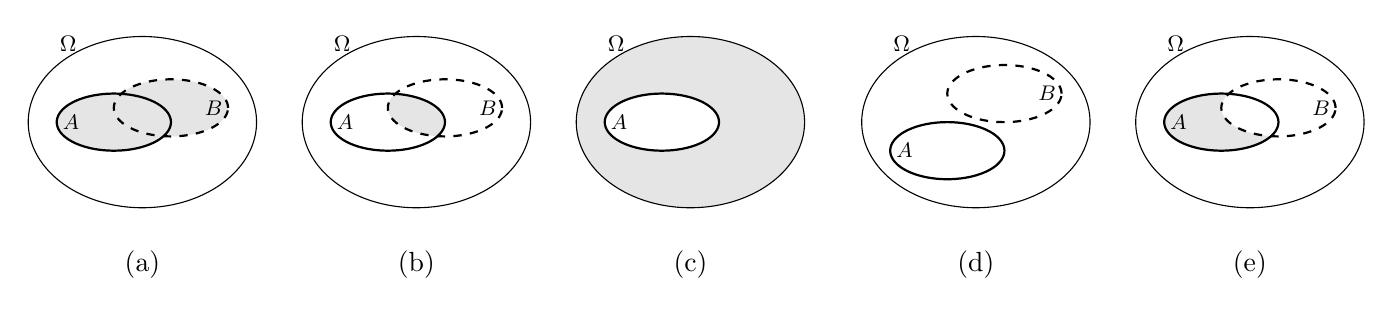
\begin{tikzpicture}[scale=.725]
\shorthandoff{>}
%
% Union y interseccion:
%
% Omega: .25*(x-.25)^2 + (y/1.5)^2 = 1
% A: x^2 + 4 y^2 = 1
% B: (x-1)^2 + 4 (y-1/4)^2 = 1
% A y B se cruzan cuando x = 1 \pm sqrt(55)/10 =>
% theta = acos(.5 \pm sqrt(55)/20) para A
% theta = acos(-.5 \pm sqrt(55)/20) para A
\pgfmathsetmacro{\s}{acos(.5-sqrt(55)/20)};
\pgfmathsetmacro{\t}{-acos(.5+sqrt(55)/20)};
\pgfmathsetmacro{\u}{-acos(-.5+sqrt(55)/20)};
\pgfmathsetmacro{\v}{acos(-.5-sqrt(55)/20)-360};
%
%
%Union
\begin{scope}
%
\fill[opacity=.1]
plot[domain=\s:\t+360,samples=200] ({cos(\x)},{.5*sin(\x)})
-- plot[domain=\u:\v+360,samples=200] ({cos(\x)+1},{.5*sin(\x)+.25})
-- cycle;
%
% borders A, B y Omega
\draw[domain=0:360,samples=200,thick] plot ({cos(\x)},{.5*sin(\x)});
\draw[dashed,domain=0:360,samples=200,thick] plot ({cos(\x)+1},{.5*sin(\x)+.25});
\draw[domain=0:360,samples=200] plot ({2*cos(\x)+.5},{1.5*sin(\x)});
%
% A, B, Omega
\draw (-.75,0) node[scale=.85]{\small $A$};
\draw(1.75,.25) node[scale=.85]{\small $B$};
\draw(-.5,1.375) node[left,scale=.9]{\small $\Omega$};
%
\draw (.5,-2.5) node{(a)};
\end{scope}
%
%
% Interseccion
\begin{scope}[xshift=4.8cm]
%
\fill[opacity=.1]
plot[domain=\s:\t,samples=200] ({cos(\x)},{.5*sin(\x)})
-- plot[domain=\u:\v,samples=200] ({cos(\x)+1},{.5*sin(\x)+.25})
-- cycle;
%
% borders A, B y Omega
\draw[domain=0:360,samples=200,thick] plot ({cos(\x)},{.5*sin(\x)});
\draw[dashed,domain=0:360,samples=200,thick] plot ({cos(\x)+1},{.5*sin(\x)+.25});
\draw[domain=0:360,samples=200] plot ({2*cos(\x)+.5},{1.5*sin(\x)});
%
% A, B, Omega
\draw (-.75,0) node[scale=.85]{\small $A$};
\draw(1.75,.25) node[scale=.85]{\small $B$};
\draw(-.5,1.375) node[left,scale=.9]{\small $\Omega$};
%
\draw (.5,-2.5) node{(b)};
\end{scope}
%
%
% Complemento
\begin{scope}[xshift=9.6cm]
%
\fill[opacity=.1]
plot[domain=0:360,samples=200] ({2*cos(\x)+.5},{1.5*sin(\x)})
-- plot[domain=0:360,samples=200] ({cos(\x)},{-.5*sin(\x)})
-- cycle;
%
% borders A y Omega
\draw[domain=0:360,samples=200,thick] plot ({cos(\x)},{.5*sin(\x)});
\draw[domain=0:360,samples=200] plot ({2*cos(\x)+.5},{1.5*sin(\x)});
%
% A, Omega
\draw (-.75,0) node[scale=.85]{\small $A$};
\draw(-.5,1.375) node[left,scale=.9]{\small $\Omega$};
%
\draw (.5,-2.5) node{(c)};
\end{scope}
%
%
% Excluyentes
\begin{scope}[xshift=14.6cm]
%
% borders A, B (con un shift...) y Omega
\draw[domain=0:360,samples=200,thick] plot ({cos(\x)},{.5*sin(\x)-.5});
\draw[dashed,domain=0:360,samples=200,thick] plot ({cos(\x)+1},{.5*sin(\x)+.5});
\draw[domain=0:360,samples=200] plot ({2*cos(\x)+.5},{1.5*sin(\x)});
%
% A, B, Omega
\draw (-.75,-.5) node[scale=.85]{\small $A$};
\draw (1.75,.5) node[scale=.85]{\small $B$};
\draw(-.5,1.375) node[left,scale=.9]{\small $\Omega$};
%
\draw (.5,-2.5) node{(d)};
\end{scope}
%
%
% privado
\begin{scope}[xshift=19.4cm]
%
\fill[opacity=.1]
plot[domain=\s:\t+360,samples=200] ({cos(\x)},{.5*sin(\x)})
-- plot[domain=\u:\v,samples=200] ({cos(\x)+1},{.5*sin(\x)+.25})
-- cycle;
%
% borders A, B y Omega
\draw[domain=0:360,samples=200,thick] plot ({cos(\x)},{.5*sin(\x)});
\draw[dashed,domain=0:360,samples=200,thick] plot ({cos(\x)+1},{.5*sin(\x)+.25});
\draw[domain=0:360,samples=200] plot ({2*cos(\x)+.5},{1.5*sin(\x)});
%
% A, B, Omega
\draw (-.75,0) node[scale=.85]{\small $A$};
\draw(1.75,.25) node[scale=.85]{\small $B$};
\draw(-.5,1.375) node[left,scale=.9]{\small $\Omega$};
%
\draw (.5,-2.5) node{(e)};
\end{scope}
%
\end{tikzpicture} \end{center}
%
\leyenda{Ilustraci\'on   de  la  operaciones   de  uni\'on   $A  \cup   B$  (a),
  intersecci\'on $A \cap B$ (b), complemento $\bar{A}$ (c), enventos excluyentes
  $A \cap B =  \emptyset$ (d). $A$ es representado en linea  llena, $B$ en linea
  discontinua; (a)-(c)  el resultado de  la operaci\'on es  la zona en  grise. A
  veces, esta representaci\'on ensemblista se  denota {\it diagrama de Venn o de
    Euler}.}
\label{fig:MP:Ensembles}
\end{figure}


Formalmente, se define  de manera abstracta un espacio  medible $(\Omega,\A)$ de
la  manera   siguiente~\cite{Hal50,  Bre88,  IbaPar97,   AthLah06,  Coh13}  (ver
tambi\'en~\cite[\&  Ref.]{BarNov78,  Bor98,  Sie18,  Sie75,  Sie76}  para  notas
hist\'oricas):
%
\begin{definicion}[Espacio medible]
  $(\Omega, \A)$ \ formado de un espacio muestral \ $\Omega$ \ y una colecci\'on
  \ $\A$  \ de conjuntos  de \  $\Omega$ \ es  llamado {\it espacio  medible} si
  satisface a los requisitos
  %
  \begin{enumerate}%[label={(\Roman*)}]
  \item $\emptyset \in \A$,
  %
  \item si $A \in \A$, entonces \ $\bar{A} \in \A$,
  %
  \item la uni\'on numerable de conjuntos de $\A$ queda en $\A$ ($\A$ es cerrado
    por la un\'ion numerable).
  %
  \end{enumerate}
  %
  Con esta propiedades, $\A$  es llamado {\it $\sigma$-\'algebra}. Los elementos
  de $\A$ son dichos {\it medibles}.
\end{definicion}
%
\noindent Es  sencillo mostrar de  que $\Omega$ tambi\'en  es en $\A$, y  de que
$\A$   est   cerrado  por   la   intersecci\'on   numerable.    Un  ejemplo   de
$\sigma$-\'algebra sobre \ $\Omega = \{ 1 \, , \,  2 \, , \, 3 \, , \, 4 \, , \,
5 \, , \, 6 \}$ \ puede ser \ $\big\{ \emptyset \, , \, \Omega \, , \, \{ 1 \, ,
\, 2 \, , \, 3 \} \, , \, \{ 4 \, , \, 5 \, , \, 6 \} \big\}$.

Las propiedades de la probabilidad $P$ de un dado evento quedan determinadas por
los siguientes (ej.~\cite{Spi76, Kol56, ShaVov06, Pla05}):

\noindent {\it Axiomas de Kolmogorov}
%
\begin{enumerate}
\item $P(A_i) \geq 0 \ \ \forall \ A_i \A$
%
\item  Si $\{ A_i  \}_i$ son  eventos mutuamente  excluyentes de  $\A$, entonces
  $\displaystyle P\left( \bigcup_i A_i \right) = \sum_i P(A_i)$
%
\item $P(\Omega) = 1$
\end{enumerate}
%
Formalmente,  se  define  un  {\it  espacio  de  probabilidad}  o  {\it  espacio
  probabil\'istico}  de   la  manera  siguiente~\cite{Hal50,   Bre88,  IbaPar97,
  AthLah06, JacPro03, Coh13}:
%
\begin{definicion}[Espacio probabil\'istico]
  Sea $(\Omega,\A)$ un espacio medible.  Una funci\'on $\mu: \A \mapsto \Rset_+$
  tal que
  %
  \begin{enumerate}
  \item $\mu(\emptyset) = 0$, y
  \item para cualquier  conjunto numerable $\{ A_i \}$  de elementos mutualmente
    excluyentes  de $\A$  se tiene  $\mu\left(  \bigcup_i A_i  \right) =  \sum_i
    \mu(A_i)$
  \end{enumerate}
  %
  es  llamada {\it  funci\'on  medida}  o {\it  medida  $\sigma$-aditiva} y  el
  espacio $(\Omega,\A,\mu)$ es  llamado {\it espacio de medida}.

  Cuando $\mu$  es acotada por  arriba, $\mu(\Omega) <  + \infty$, la  medida es
  dicha  {\it  finita} y  el  espacio tambi\'n  es  dicho  finito. Adem\'as,  si
  \[ P \equiv  \mu, \quad \P(\Omega) = 1  \], la medida es dicha  medida de {\it
    probabilidad}, $\mu \equiv P$.  En  este caso, el espacio $(\Omega,\A,P)$ es
  llamado {\it espacio probabil\'istico}.
\end{definicion}


A  partir de  los axiomas  de Kolmogorov  se pueden  probar varios  corolarios y
propiedades:
%
\begin{itemize}
\item la probabilidad de un evento seguro o cierto es 1;
%
\item  la   probabilidad  de   un  evento   que  no  puede   ocurrir  es   0:  \
  $P(\emptyset) = 0$;
%
\item el rango  de las probabilidades est\'a  acotado: \ $0 \leq P(A)  \leq 1\ \
  \forall \ A \in \A$;
%
\item condici\'on de  normalizaci\'on: \ si $\Omega =  \bigcup_{i=1}^n A_i$, con
  $A_i$  mutuamente  excluyentes,  entonces  \  $\sum_{i=1}^n P(A_i)  =  1$;  el
  conjunto  $\{ A_i  \}_{i=1}^n$  es  dicho {\it  conjunto  completo de  eventos
    posibles      excluyentes      entre      s\'i}     y      es      ilustrado
  figure~\ref{fig:MP:CompletoSub};
%
\item si $A$ es subconjunto de $B$,  lo que escribiremos $A \subset B$, es decir
  si  $B$  se realiza,  $A$  se realiza  tambi\'en  (pero  no necesariamente  al
  rev\'es),     entonces     \     $P(A)     \leq    P(B)$;     Es     ilustrado
  figure~\ref{fig:MP:CompletoSub};
\end{itemize}

\begin{figure}[h!]
\begin{center} 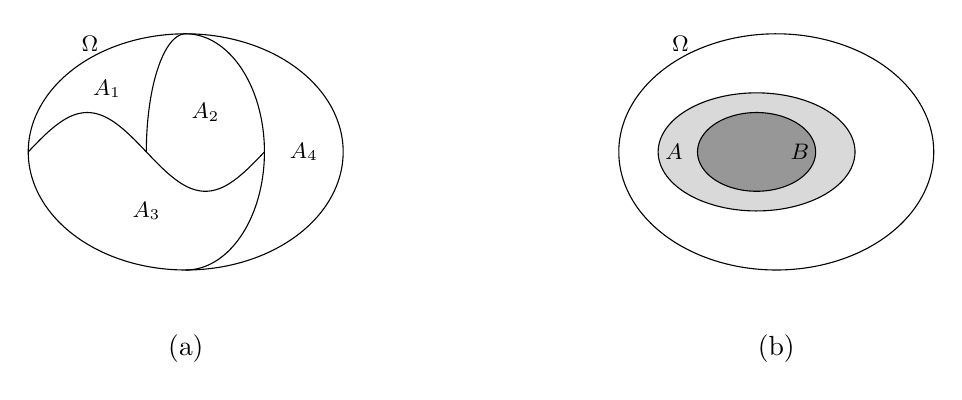
\begin{tikzpicture}%[scale=.9]
\shorthandoff{>}
%
% Particion
\begin{scope}
%
% Omega y A_i
\draw[domain=0:360,samples=200] plot ({2*cos(\x)+.5},{1.5*sin(\x)});
\draw[domain=-90:90,samples=200] plot ({cos(\x)+.5},{1.5*sin(\x)});
\draw[domain=90:180,samples=200] plot ({.5*cos(\x)+.5},{1.5*sin(\x)});
\draw[domain=0:3,samples=200] plot (\x-1.5,{.5*sin(120*\x)});
%
%
% Omega y A_i's
\draw(-.5,1.375) node[left,scale=.9]{\small $\Omega$};
\draw(-.5,.8) node[scale=.9]{\small $A_1$};
\draw(.75,.5) node[scale=.9]{\small $A_2$};
\draw(0,-.75) node[scale=.9]{\small $A_3$};
\draw(2,0) node[scale=.9]{\small $A_4$};
%
\draw (.5,-2.5) node{(a)};
\end{scope}
%
%
% Inclusion
\begin{scope}[xshift=7.5cm]
%
\fill[opacity=.15] plot[domain=0:360,samples=200] ({1.25*cos(\x)+.25},{.75*sin(\x)});
\fill[opacity=.3] plot[domain=0:360,samples=200] ({.75*cos(\x)+.25},{.5*sin(\x)});
%
% borders A, B y Omega
\draw[domain=0:360,samples=200] plot ({1.25*cos(\x)+.25},{.75*sin(\x)});
\draw[domain=0:360,samples=200] plot ({.75*cos(\x)+.25},{.5*sin(\x)});
\draw[domain=0:360,samples=200] plot ({2*cos(\x)+.5},{1.5*sin(\x)});
%
% A, B, Omega
\draw (-.8,0) node[scale=.9]{\small $A$};
\draw(.8,0) node[scale=.9]{\small $B$};
\draw(-.5,1.375) node[left,scale=.9]{\small $\Omega$};
%
\draw (.5,-2.5) node{(b)};
\end{scope}
%
\end{tikzpicture} \end{center}
%
\leyenda{Ilustraci\'on  de  conjunto completo  de  eventos posibles  excluyentes
  entre s\'i  (a), y de  la inclusi\'on  (b) donde $A$  es en grise  (claro como
  oscuro) mientras de que $B$ es en grise oscuro.}
\label{fig:MP:CompletoSub}
\end{figure}

Nota:  la probabilidad  \ $P(A  \cap B)$  \ del  evento $A  \cap B$  \  se llama
tambi\'en {\it probabilidad conjunta} de \ $A$ \ y \ $B$.
%$P(A  \cap B)  = P(B  \cap A)$}  es la
%probabilidad del evento conjunto dado por  la composici\'on de los eventos $A$ y
%$B$. 

Se demuestra que
%
\begin{itemize}
\item $P(A  \cap B)$ est\'a acotada:  \ $0 \leq P(A  \cap B) \leq  \min\{ P(A) ,
  P(B)\}$; (viene de \ $A \cap B \subset A$ \ y \ $A \cap B \subset B$).
%
\item Si  $A$ y $B$ son  mutuamente excluyentes, entonces  \ $p(A \cap B)  = 0$;
  (viene de \ $A \cap B = \emptyset$).
%
\item  si  $\{ B_j  \}_{j=1}^m$  es un  conjunto  completo  de eventos  posibles
  excluyentes entre s\'i, entonces \ $\sum_{j=1}^m P(A \cap B_j) = P(A)$; (viene
  de  $\{ A  \cap B_j  \}$ mutualmente  excluyentes y  $\bigcup_j \left(  A \cap
    B_j\right) = A \cap \left( \bigcup_j B_j \right) = A \cap \Omega = A$).
\end{itemize}

En el caso de eventos no necesariamente mutuamente excluyentes, se prueba que la
{\it ley de composici\'on} o {\it formula de inclusi\'on-exclusi\'on} es
%
\[
P(A \cup B) = P(A) + P(B) - P(A \cap B) \leq P(A) + P(B), 
\]
%
y que para $n$ eventos resulta
%
\[
P\left( \bigcup_{i=1}^n A_i \right) \leq \sum_{i=1}^n P\left( A_i \right).
\]
%
La  igualdad  vale  en  el  caso  especial  de  eventos  mutuamente  excluyentes
(recuperando el segundo axioma de Kolmogorov).

Se  prueba tambi\'en  de que  si $\{  A_i \}_{i=1}^{+\infty}$  es  una secuencia
creciente  de eventos,  \ie $\forall  \, i  \ge 1,  \quad A_i  \subset A_{i+1}$,
entonces
%
\[
P\left( \bigcup_{i=1}^{+\infty} A_i \right) = \lim_{i \to +\infty} P(A_i)
\]
%
Similarmente,  si $\{ A_i  \}_{i=1}^{+\infty}$ es  una secuencia  decreciente de
eventos, \ie $\forall \, i \ge 1, \quad A_{i+1} \subset A_i$, entonces
%
\[
P\left( \bigcap_{i=1}^{+\infty} A_i \right) = \lim_{i \to +\infty} P(A_i)
\]


Se puede preguntarse de cual es la probabilidad de un evento $A$, si sabemos que
tenemos un evento $B$, dado.  Por  ejemplo, por un dado de 6 caras equilibriado,
cual es la probabilidad de tener  un n\'umero par sabiendo que tenemos un numero
menor  a igual  a  3.   La respuesta  es  en la  noci\'on  de {\it  probabilidad
  condicional}~\cite{Hau01, Jef48, Jef73, Bre88, ManWol95, JacPro03, ShaVov06}:
%
\begin{definicion}[Probabilidad condicional]
  \underline{Por definici\'on},  la {\it  probabilidad condicional} de  $A$ dado
  $B$ es la raz\'on entre la  probabilidad del evento conjunto y la probabilidad
  de que se d\'e $B$ (cuando \'este es un evento no nulo):
  %
  \[
  P(A|B) = \frac{P(A \cap B)}{P(B)}.
  \]
\end{definicion}
%
En  el  ejemplo precediente,  la  probabilidad  va a  ser  $P(A|B)  = \frac13  =
\frac{\frac16}{\frac12}  = \frac{P(A  \cup B)}{P(B)}$. 

Es f\'acil demostrar %% <-- ejercicio
que esta  cantidad toma valores  entre 0 y  1, con $P(\Omega|B)  = 1$, y  que es
aditiva  para  una  uni\'on  de  eventos  mutuamente  excluyentes  referidos  al
cumplimiento de $B$.  Luego, $P(A|B)$ es una medida de probabilidad~\footnote{Se
  puede  definir un  espacio de  probabilidad $(  \Omega_B, \A_B  ,  P_B)$ donde
  $P_B(A)  \equiv P(A|B)$.};  Por eso,  a veces  en la  literatura se  la denota
$P_B(A)$.  Diversas  situaciones de probabilidades  condicionales son ilustradas
en la figura siguiente, Fig.~\ref{fig:MP:Condicional}.

\begin{figure}[h!]
\begin{center} 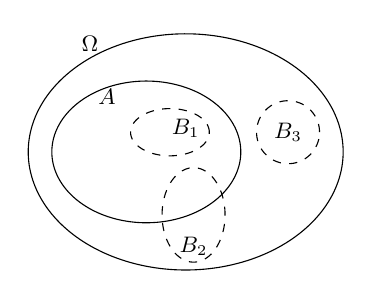
\begin{tikzpicture}%[scale=.9]
\shorthandoff{>}
%
\begin{scope}
%
% Omega, A, B_i
\draw[domain=0:360,samples=200] plot ({2*cos(\x)+.5},{1.5*sin(\x)});
\draw[domain=0:360,samples=200] plot ({1.2*cos(\x)},{.9*sin(\x)});
\draw[dashed,domain=0:360,samples=200] plot ({.5*cos(\x)+.3},{.3*sin(\x)+.25});
\draw[dashed,domain=0:360,samples=200] plot ({.4*cos(\x)+.6},{.6*sin(\x)-.8});
\draw[dashed,domain=0:360,samples=200] plot ({.4*cos(\x)+1.8},{.4*sin(\x)+.25});
%
%
% Omega y A_i's
\draw(-.5,1.375) node[left,scale=.9]{\small $\Omega$};
\draw(-.5,.7) node[scale=.9]{\small $A$};
\draw(.5,.3) node[scale=.9]{\small $B_1$};
\draw(.6,-1.2) node[scale=.9]{\small $B_2$};
\draw(1.8,.25) node[scale=.9]{\small $B_3$};
%
\end{scope}
%
\end{tikzpicture} \end{center}
%
\leyenda{Ilustraci\'on  de  la probabilidad  condicional  con  $A$ interior  del
  elipse  en linea  llena  y unos  $B_i$  interiores de  los  elipses en  lineas
  discontinuas.   \ $\omega  \in B_1  \Rightarrow \omega  \in A$  \ as\'i  que \
  $P(A|B_1) = 1$. Al rev\'es, \  $\omega \in B_3 \Rightarrow \omega \not\in A$ \
  as\'i que \  $P(A|B_3) = 0$.  Entre estas  situaciones extremas, si $P(\bar{A}
  \cap B_2)  \ne 0$ \ y  \ $P(A \cap  B_2) \ne 0$ \  tenemos $0 < P(A|B_2)  < 1$
  (ej.  con   probabilidades  iguales  a   las  superficias  relativas   de  los
  conjuntos).}
\label{fig:MP:Condicional}
\end{figure}

Algunas propiedades interesantes son las siguientes:
%
\begin{itemize}
\item condici\'on  de normalizaci\'on: \  $\sum_{i=1}^n P(A_i|B) = 1$,  siendo \
  $\{ A_i \}_{i=1}^n$  \ un conjunto completo de  resultados posibles mutuamente
  excluyentes;
%
\item relaci\'on  entre probabilidades condicionales  inversas: \ $\displaystyle
  P(B|A)  = \frac{P(B)}{P(A)}  P(A|B)$, de  donde \  $p(A|B)$ \  y \  $p(B|A)$ \
  coinciden s\'olo cuando \ $A$ \ y \ $B$ \ tienen la misma probabilidad;
%
\item {\it f\'ormula de probabilidades totales}: \ si $\{ B_j \}$ es un conjunto
  completo de eventos no nulos mutuamente excluyentes, entonces
  %
  \[
  P(A) = \sum_j P(A|B_j) P(B_j)
  \]
  %
  Viene de \ $A = A \cap  \left( \bigcup_j B_j \right) = \bigcup_j \left( A \cap
    B_j \right)$  \ donde  los \ $A  \cap B_j$  \ son mutuamente  excluyentes, y
  $P\left( A \cap B_j \right) = P(A|B_j) P(B_j)$.
%
\item {\it  f\'ormula de Bayes}:  \ si  $\{ B_j \}$  es un conjunto  completo de
  eventos no nulos mutuamente excluyentes, entonces
  %
  \[
  P(B_i|A) = \frac{P(A \cap B_i)}{P(A)} = \frac{P(A|B_i) P(B_i)}{\sum_j P(A|B_j)
    P(B_j)} .
  \]
  %
  (ver~\cite{Bre88, JacPro03, Bay63, Bar58}).
\end{itemize}

Terminamos  esta   secci\'on  por  la   noci\'on  de  independencia   entre  dos
eventos. Por ejemplo, si dos dados son tirado sobre dos mesas diferentes, no hay
ninguna raz\'on de que la muestra de  uno ``influye'' la del otro. Dicho de otra
manera,  dos  eventos  son  inde�ndientes  si conciendo  uno  no  lleva  ninguna
``informaci\'on'' sobre el otro~\cite{Bre88, ManWol95, Hau01, JacPro03, Bor09}:
%
\begin{definicion}[Independencia estad\'istica]
  Dos eventos \ $A$ \ y \ $B$ \ se dicen {\it estad\'isticamente independientes}
  si la  probabilidad condicional  de $A$  dado $B$ es  igual a  la probabilidad
  incondicional de $A$:
  %
  \[
   P(A|B) = P(A).
   \]
  %
   Es equivalente al hecho de que la probabilidad conjunta se factoriza,
  %
  \[
   P(A \cap B) = P(A) P(B).
   \]
\end{definicion}
%
Por  inducci\'on, la  condici\'on necesaria  y suficiente  para que  $n$ eventos
$A_1,\ldots,A_n$ sean  estad\'isticamente independientes es  que la probabilidad
conjunta se factorice como
%
\[
P\left( \bigcap_{i=1}^n A_i \right) = \prod_{i=1}^n P(A_i).
\]
%
Se  deduce que  los  eventos mutuamente  excluyentes  no son  estad\'isticamente
independientes.

% ============ Variables aleatorias y distribuciones de probabilidad =========== %

\seccion{Variables aleatorias y distribuciones de probabilidad}
\label{s:variablealeatoria}


\SZ{\cite[\& Ref.]{BarNov78}}



%%%%%%%%%%%%%%%%%%%%%%%%%%%%%%%%%%%%%%%%%%%%%%%%%%%%%%%%%%%%%%%%%%%%%%%%%%

\emph{En  un  experimento  o  un  dado  proceso,  los  posibles  resultados  son
  t\'ipicamente  n\'umeros reales, siendo  cada n\'umero  un evento.   Luego los
  resultados  son mutuamente  excluyentes. Se  considera a  esos  n\'umeros como
  valores de una  \emph{variable aleatoria} $X$ a valores  reales, que puede ser
  discreta  (cuando  el espacio  muestral  es  finito  o infinito  numerable)  o
  continua.  La ley  de la variable aleatoria $X$ es  una medida de probabilidad
  definida por  \ $P_X(x) =  \Pr(X=x)$ o, en  general, por $P_X(A)  = \Pr(X=x\in
  A)$.  Para indicar  que la variable~$X$ sigue la ley  de distribuci\'on $p$ se
  escribe  \  $X\sim p  $.   Puede  ser  \'util tambi\'en  considerar  variables
  aleatorias  complejas  $Z=X+iY$, donde  $X$  e  $Y$  son variables  aleatorias
  reales. }

%%%%%%%%%%%%%%%%%%%%%%%%%%%%%%%%%%%%%%%%%%%%%%%%%%%%%%%%%%%%%%%%%%%%%%%%%%
\subseccion{Variable aleatoria discreta}

Los  posibles valores de  una variable  aleatoria discreta  $X$ consisten  en un
conjunto  contable  (finito  o   infinito  numerable)  de  n\'umeros  reales:  \
$x\in\Omega=\{x_1,   x_2,  \ldots\}$.   A   cada  uno   de  los   valores  $x_n$
($n=1,2,\ldots$) se puede asociar una  probabilidad $p_n=p(x_n)$, de modo que se
satisface la condici\'on de normalizaci\'on:
%
$$\sum_n p_n = 1 . $$ 
%
La \emph{funci\'on (de masa) de probabilidad} es  de la forma: 
%
$$
p(x) = \left\{
\begin{array}{cl}
\Pr(X=x) & \mbox{si} \ x=x_1, x_2, \ldots \\ 0 &
\mbox{en~todo~otro~punto}
\end{array} \right.
$$
%
En  la   Fig.~\ref{fig:distribprobdiscreta}  se  muestra   una  representaci\'on
gr\'afica de una distribuci\'on de probabilidad discreta.
%
\begin{figure}[h!] %%ojo numeracion de figs !
%\centerline{\includegraphics[width=3cm]{distribprobdiscreta.jpg}} %%rehacer
%
\leyenda{Una distribuci\'on de probabilidad discreta.}
\label{fig:distribprobdiscreta}
\end{figure}

Tambi\'en, se puede caracterizar la ley de la variable discreta $X$ por medio de
su \emph{funci\'on de repartici\'on}:
%
$$
F_X(x)= \Pr(X\in(-\infty,x]) = \Pr (X\leq x) = \sum_{\forall
  n \,:\, x_n\leq x} p(x_n)
$$
%
que es una funci\'on discontinua, con saltos finitos, y no decreciente. 

Sin  p\'erdida de  generalidad, el  conjunto de  valores que  toma  una variable
aleatoria discreta $X$ puede considerarse como $\{0,1,2,\ldots,N\}$ para alg\'un
$N$ natural, o todo $\Nset$. Entonces la ley de una variable aleatoria a valores
naturales est\'a dada por  \ $\{p_n = \Pr(X=n), \ n\in \Nset  \}$.  Luego \ $\Pr
(X\in  A)=\sum_{n\in A\cap  \Nset}  p_n$,  y la  funci\'on  de repartici\'on  se
calcula como  \ $\Pr(X\leq x) = \sum_{n  \leq x} \Pr(X=n)$ que  es una funci\'on
que presenta un  salto finito en cada n\'umero natural.  En  general un salto de
la funci\'on  de repartici\'on corresponde a  la presencia de  una \emph{masa de
  Dirac} en el entorno del salto. %%

Un caso especial se tiene cuando un  valor $x_j$ es cierto o seguro, y no ocurre
ninguno de  los otros valores $x_i \  (i\neq j)$. La forma  de la distribuci\'on
es: \ $p_n=\delta_{nj}$, donde
%
$$
\delta_{ij} = \left\{
\begin{array}{cl}
1 & \mbox{si} \ i=j \\
0 & \mbox{si} \ i\neq j 
\end{array} \right.
$$
%
es el s\'imbolo \emph{delta de  Kronecker}. Cuando el espacio muestral es finito
de dimensi\'on $N$, la ley de  distribuci\'on se puede representar por medio del
siguiente vector columna:
%
$$
p = \begin{pmatrix}
% \left(  
%\begin{array}{c}
0 \\ \vdots \\ 0 \\ 1  \\ 0 \\ \vdots \\ 0
\end{pmatrix}
%\end{array} \right)
$$
%
con  un  1  en  el  lugar  $j$-\'esimo,  que tambi\'en  se  escribe  como  \  $p
= \begin{pmatrix} 0  & \cdots & 0 &  1 & 0 & \cdots &  0 \end{pmatrix}^t$, donde
$t$ indica transposici\'on.  La funci\'on de repartici\'on resulta una funci\'on
escal\'on o de Heaviside: \ $F(x)=\Theta(x-x_j)$.

Otra    situaci\'on   particular    es   la    de    \emph{equiprobabilidad}   o
\emph{distribuci\'on uniforme}.  La forma  de la distribuci\'on es: \ $p_n=\frac
1N \ \ \forall\ n=1,\ldots,N$, donde  $N$ se�ala el tama�o del espacio muestral.
La ley  de distribuci\'on  se puede representar  por medio del  siguiente vector
columna:
%
$$
p = \begin{pmatrix}
% \left(  
%\begin{array}{c}
1/N \\ 1/N  \\ \vdots \\ 1/N
\end{pmatrix}
%array} \right) , 
$$
%
que tambi\'en se escribe como \  $p = \begin{pmatrix} \frac1N & \frac1N & \cdots
  &  \frac1N  \end{pmatrix}^t$.   La  funci\'on  de  repartici\'on  resulta  una
funci\'on escalonada,  con saltos de  altura $\frac1N$ para  cada $n$ entre  1 y
$N$.

\hfill 

\emph{Reordenamiento y relaci\'on de mayorizaci\'on} 

Para comparar dos  distribuciones es \'util reordenar el  vector de probabilidad
permutando  sus  elementos  hasta  listarlos  de forma  descendente.   Se  anota
$p^\downarrow$, de  modo que \  $p^\downarrow_1 \geq p^\downarrow_2  \geq \ldots
\geq  p^\downarrow_N$.   En  el  ejemplo   del  caso  con  certeza  se  tiene  \
$p^\downarrow =  \begin{pmatrix} 1 & 0  & \cdots &  0 \end{pmatrix}^t$, mientras
que la distribuci\'on uniforme no var\'ia.

Se  define  \emph{mayorizaci\'on} del  siguiente  modo,  para distribuciones  de
dimensi\'on  $N$ (con  sus elementos  acomodados  en forma  decreciente): \  una
distribuci\'on $p$  es mayorizada por otra $q$,  y se denota $p\prec  q$, si las
primeras $N-1$  sumas parciales de $p^\downarrow$ y  $q^\downarrow$ satisfacen \
$\sum_{i=1}^n  p^\downarrow_i   \leq  \sum_{i=1}^n  q^\downarrow_i$   para  todo
$n=1,\ldots,N-1$, con \ $\sum_{i=1}^N p_i = 1 = \sum_{i=1}^N q_i$.

Por    ejemplo,   $\begin{pmatrix}    \frac12    &   \frac14    &   \frac18    &
  \frac18 \end{pmatrix}^t  \prec \begin{pmatrix} \frac12  & \frac14 &  \frac14 &
  0 \end{pmatrix}^t$.  Es posible  comparar por mayorizaci\'on distribuciones de
distinta  dimensionalidad, completando con  ceros el  vector de  probabilidad de
menor  dimensi\'on.  Es  importante  resaltar que  la  mayorizaci\'on provee  un
\emph{orden  parcial}  (no  total)  entre distribuciones,  existiendo  pares  de
distribuciones   tales  que   ninguna  mayoriza   a  la   otra.    Por  ejemplo,
$\begin{pmatrix} 0.50 &  0.40 & 0.10 \end{pmatrix}^t$ y  $\begin{pmatrix} 0.70 &
  0.15 & 0.15 \end{pmatrix}^t$ no se comparan por mayorizaci\'on.

Es  interesante  notar  que  la   siguiente  propiedad  es  v\'alida  para  toda
distribuci\'on $p$ de tama�o~$N$:
%
$$
\begin{pmatrix} \frac1N & \frac1N & \cdots & \frac1N \end{pmatrix}^t \ \prec \ p
\ \prec \ \begin{pmatrix} 1 & 0 & \cdots & 0 \end{pmatrix}^t.
$$
%
En este  sentido, los  casos particulares de  equiprobabilidad y de  certeza, se
dice  que  son  distribuciones  extremas.  Notamos que  uno  implica  ignorancia
m\'axima  en el  resultado de  la variable  mientras que  el otro  corresponde a
conocimiento completo.
%% graficamente 
%
\begin{figure}[h!] %%ojo numeracion de figs !
%\centerline{\includegraphics[width=3cm]{majorizationplot.pdf}} %%rehacer
%
\leyenda{Orden parcial por mayorizaci\'on}
\label{fig:majorizationplot}
\end{figure}

%%%%%%%%%%%%%%%%%%%%%%%%%%%%%%%%%%%%%%%%%%%%%%%%%%%%%%%%%%%%%%%%%%%%%%%%%%
\subseccion{Variable aleatoria continua}

\SZ{\cite[\& Ref.]{BarNov78}}

Los posibles valores de una  variable aleatoria continua $X$ son cualesquiera de
los n\'umeros en un dado  intervalo de la recta real: \ $x\in\Omega\subset\Rset$
que  puede ser  un intervalo  $[x_m,x_M]$  o un  subconjunto (semi)infinito.  Es
conveniente asociar una  \emph{funci\'on densidad de probabilidad} (com\'unmente
anotada por su  sigla en ingl\'es: pdf por  \emph{probability density function})
$p(x)$ que tiene el  sentido de que la probabilidad de que  $X$ tome valor entre
$a$ y $b$ est\'a dada por:
%
$$
\Pr(a\leq X\leq b) = \int_a^b p(x) \, dx ,
$$
%
siendo $p(x)  \, dx$  la densidad de  probabilidad de  hallar a la  variable con
valores  en el intervalo  infinitesimal entre  $x$ y  $x+dx$. La  condici\'on de
normalizaci\'on se escribe
%
$$
\int_{x_m}^{x_M} p(x) \, dx=1 . 
$$ 

En  la   Fig.~\ref{fig:distribprobcontinua}  se  muestra   una  representaci\'on
gr\'afica de una funci\'on densidad de probabilidad para una variable continua.
%
\begin{figure}[h!] %%ojo numeracion de figs !
%\centerline{\includegraphics[width=3cm]{distribprobcontinua.png}} %%rehacer
%
\leyenda{Una distribuci\'on de probabilidad continua.}
\label{fig:distribprobcontinua}
\end{figure}

Tambi\'en, se puede caracterizar la ley de la variable continua $X$ por medio de
su  \emph{funci\'on  de   repartici\'on}  o  \emph{funci\'on  de  distribuci\'on
  cumulativa} (CDF por \emph{cumulative distribution function}):
%
$$
F_X(x) = \Pr(X\leq x) = \int_{x_m}^x p(t) \, dt
$$
%
que da la  probabilidad de que $X$ sea  menor o igual que cierto  valor $x$ dado
(dentro del conjunto~$\Omega$ de todos  los valores posibles de la variable). En
forma an\'aloga,  \ $\Pr(X\in  A) = \int_A  p(x) \,  dx$ acumula la  densidad de
probabilidad en un subconjunto $A$ del espacio muestral.  Por la propiedad de la
inclusi\'on,  se  tiene \  $\Pr(X\leq  x_1)  \leq  \Pr(X\leq x_2)$  siempre  que
$x_1\leq x_2$; luego $F_X(x)$ es una funci\'on creciente
%%no decreciente ?? SI, LO DIRIA ASI
de   $x$,  acotada   por  la   unidad,  con   valores  extremos   dados   por  \
$\lim_{x\rightarrow -\infty} F_X(x)=0$  y $\lim_{x\rightarrow \infty} F_X(x)=1$,
tomando $\Omega=\Rset$.  Adem\'as la derivada respecto de $x$ es la pdf:
%
$$
\frac{dF_X(x)}{dx}=p(x) . 
$$ 
%
De aqu\'i  se observa que  la densidad de  probabilidad $p(x)$ puede no  ser una
funci\'on ``ordinaria''  cuando $\Pr(X\leq x)$  es discontinua, pero  como mucho
tiene  la  singularidad  de   una  distribuci\'on  \emph{delta  de  Dirac}  cuya
representaci\'on integral es:
%
$$
\delta (x) = \frac{1}{2\pi} \int_{-\infty}^{\infty} e^{itx} dt . 
$$
% SZ: LA  VERDAD ES  QUE NO ME  GUSTA MUCHO  escribir una distribucion  como una
% fuccion porque no viven en el  mismo espacio. Pero no importa. Para mi, cuando
% hay  una  discontinuidad  X no  admite  une  pdf  por  definicion del  'f'  de
% pdf\sum_{}

Un caso especial  se tiene cuando la variable aleatoria $X$  toma el valor $x_0$
con certeza.  La forma  de la pdf  es: \ $p(x)=\delta(x-x_0)$.  Otra situaci\'on
particular es la distribuci\'on uniforme en  un intervalo; la pdf es de la forma
\  $p(x)=\frac{1}{b-a} \  \forall  \  x\in[a,b]$, donde  $[a,b]$  es el  espacio
muestral.

Usando las  funciones delta de  Dirac, se puede  unificar el tratamiento  de las
variables  aleatorias discretas  con las  continuas: si  una  variable aleatoria
discreta  toma los  valores $x_1,  x_2,  \ldots$ con  probabilidades $p_1,  p_2,
\ldots$ respectivamente,  entonces formalmente  se puede describir  mediante una
variable  aleatoria  continua  $X$  con  funci\'on densidad  de  probabilidad  \
$p(x)=\sum_j p_j \,\delta(x-x_j)$.


%%%%%%%%%%%%%%%%%%%%%%%%%%%%%%%%%%%%%%%%%%%%%%%%%%%%%%%%%%%%%%%%%%%%%%%%%%
\subseccion{Vector aleatorio}


Cuando se trabaja  con $d\geq 2$ variables aleatorias  es conveniente definir un
\emph{vector aleatorio} de dimensi\'on $d$,  y apelar para su estudio a nociones
del \'algebra  lineal y  a notaci\'on matricial.   Se tiene el  vector aleatorio
$d$-dimensional  \  $\mathbf{X} =  \{X^1,  \ldots,  X^d  \}$, o  simplemente  $X
=  \begin{pmatrix}  X^1  &  \cdots  & X^d  \end{pmatrix}^t$,  caracterizado  por
$d$-uplas de variables aleatorias reales, con funci\'on densidad de probabilidad
conjunta~$p(x^1, \ldots, x^d)$. La ley  del vector $\mathbf{X}$ es una medida de
probabilidad sobre $\Rset^d$, con
%
$$
P_{\mathbf{X}}(\mathbf{A})  =   \Pr(\mathbf{X}\in\mathbf{A})  =  \int_{\mathbf{A}}
p(x^1, \ldots, x^d)\ dx^1\ldots dx^d
$$
%
para  $\mathbf{A}  \subset \mathbf{\Omega}$,  siendo  la  pdf  conjunta $p$  una
funci\'on positiva, definida sobre $\mathbf{\Omega}\subset\Rset^d$, y tal que se
satisface la condici\'on de normalizaci\'on:
%
$$
\int_{\mathbf{\Omega}} p(x^1, \ldots, x^d)\ dx^1\ldots dx^d  = 1 .
$$

La  \emph{funci\'on densidad  de  probabilidad marginal}  que  caracteriza a  la
variable aleatoria  $X^i$ es la  ley que se  obtiene integrando la  pdf conjunta
sobre todas las variables excepto la $i$-\'esima:
%
$$
p_{X^i}(x^i)  =  \int_{\mathbf{\Omega}^{(i)}}  p(x^1, \ldots,  x^d)\  dx^1\ldots
dx^{i-1} dx^{i+1} \ldots dx^d
$$
%
donde $\mathbf{\Omega}^{(i)}\subset\Rset^{d-1}$  barre el espacio  muestral para
$X^1, \ldots, X^{i-1}, X^{i+1}, \ldots, X^d$.

Las  $d$  variables  aleatorias  $X^1,  \ldots,  X^d$  de  un  vector  aleatorio
$\mathbf{X}$ se dicen \emph{independientes} si corresponden a eventos mutuamente
independientes. Esto se  da si y s\'olo  si la pdf conjunta se  factoriza en las
$d$ pdf marginales:
%
$$
p(x^1, \ldots, x^d) = p_{X^1}(x^1) \cdots p_{X^d}(x^d) . 
$$


%%%%%%%%%%%%%%%%%%%%%%%%%%%%%%%%%%%%%%%%%%%%%%%%%%%%%%%%%%%%%%%%%%%%%%%%%%
\subseccion{Transformaci\'on de variables aleatorias}


Sea $X$ una  variable aleatoria (continua, en general)  definida en el intervalo
$[x_m, x_M]$ con funci\'on densidad  de probabilidad $p(x)$. Sea $Y=\Psi(X)$ una
funci\'on real  de $X$, luego $Y$  toma los valores $y=\Psi(x)$  en el intervalo
$[y_m,y_M]$.  La funci\'on  densidad  de probabilidad  $q(y)$  para la  variable
aleatoria transformada $Y$ se obtiene  de la siguiente manera, dependiendo de la
forma de la transformaci\'on:

\begin{itemize}
\item Si  $\Psi$ es inversible, con  inversa (\'unica), se  tiene \ $x=\Phi(y)$,
  con  $\Phi=\Psi^{-1}$.  A partir  de  la  propiedad  de conservaci\'on  de  la
  probabilidad
  %
  $$
  |q(y)\, dy| = |p(x) \, dx|
  $$ 
  %
  para  una correspondencia  biun\'ivoca  entre $x$  e  $y$, se  obtiene la  pdf
  transformada
  %
  $$
  q(y)  = p(x)  \left| \frac{dx}{dy}  \right| =  p\left(\Phi(y)\right)  \ \left|
    \Phi'(y)   \right|   =  \frac{p\left(\Phi(y)\right)}{\left|   \Psi'(\Phi(y))
    \right|} .
  $$
  %
  Una forma alternativa  de derivar este resultado es partir  de la funci\'on de
  repartici\'on:
  %
  $$
  F_Y(y)  =  P(Y\leq  y)  =  P(\Psi(X)  \leq  y)  =  P(X\leq  \Psi^{-1}  (y))  =
  F_X(\Phi(y))
  $$
  %
  y  calcular las  derivadas del  primer y  \'ultimo t\'erminos  respecto  de la
  variable transformada~$y$.
%
\item Si la inversa de $\Psi$  es multivaluada, cada valor de $y$ se corresponde
  con  un conjunto de  valores de  $x$, digamos  $\{x_k =  \Phi_k(y), \  k=1, 2,
  \ldots\}$.  Debido a  que  estas soluciones  son  mutuamente excluyentes,  las
  probabilidades se suman, de modo que
  %
  $$
  q(y)   =    \sum_k   p(x_k)   \left|   \frac{dx_k}{dy}    \right|   =   \sum_k
  \frac{p\left(\Phi_k(y)\right)}{\left| \Psi'(\Phi_k(y)) \right|} ,
  $$
  %
  que   formalmente  se   puede  expresar   como  \   $q(y)  =   \int   p(x)  \,
  \delta(y-\Psi(x)\,) \ dx$ , donde se  usa la expansi\'on de la funci\'on delta
  en  t\'erminos de sus  ceros: \  $\delta(y-\Psi(x)\,)= \sum_k  \delta(x-x_k) /
  |\Psi'(x_k)| $.\newline  Por ejemplo, para la transformaci\'on  de variables \
  $Y=X^2$ se tiene \  $Y=\Psi(X)=X^2$ cuyas inversas son \ $X_1=\Phi_1(Y)=+\sqrt
  Y$  y   $X_2=\Phi_2(Y)=-\sqrt  Y$;  luego   \  $q(y)=\frac{p(\sqrt  y)}{2\sqrt
    y}+\frac{p(-\sqrt y)}{|-2\sqrt y|}$ , para $y>0$.
\end{itemize}

\hfill

Consideramos ahora el  caso de un vector aleatorio  $\mathbf{X} = \{X^1, \ldots,
X^d\}$  con  funci\'on  densidad  de  probabilidad conjunta  \  $p(x^1,  \ldots,
x^d)$. Se  define otro vector aleatorio  \ $\mathbf{Y} =  \{Y^1, \ldots, Y^d\}$,
por   medio   de   las   transformaciones  \   $Y^j=\Psi^j(X^1,\ldots,X^d)$,   \
$j=1,\ldots,d$. Suponiendo que las  funciones $\Psi^j$ tienen inversa (\'unica),
se  puede escribir \  $X^j=\Phi^j(Y^1,\ldots,Y^d)$ para  cada $j$.  La funci\'on
densidad de probabilidad conjunta $q(y^1,\ldots,y^d)$ para $\mathbf{Y}$ se puede
obtener a partir de la propiedad de conservaci\'on de la probabilidad
%
$$
|q(y^1,\ldots,y^d)\ dy^1\cdots dy^d| = |p(x^1,\ldots,x^d) \ dx^1\cdots dx^d| .
$$ 
%
Para  una  correspondencia biun\'ivoca  entre  $\mathbf{x}$  e $\mathbf{y}$,  se
obtiene la pdf transformada
%
$$
q(y^1,\ldots,y^d) = \left| \Jac_\Phi \right| \, p(x^1,\ldots, x^d) 
%%= \int  p(x^1,\ldots, x^d) \delta(y^1-\Psi^1) .......  dx^1 .....
$$
%
donde  $\Jac_\Phi =  \frac{\partial(\Phi^1  , \ldots  , \Phi^d)}{\partial(y^1  ,
  \ldots , y^d)}$ es el Jacobiano de la transformaci\'on.

%% Ejercicio: Estudiar el caso multivaluado / Resolver un ej. 

\hfill

Una  \emph{variable  aleatoria  compleja}   $Z=X+i  Y$  puede  interpretarse  en
t\'erminos de las  dos variables aleatorias reales $X$ e $Y$.  La pdf asociada \
$P(z)=p(x,y)$ est\'a dada por la  funci\'on densidad de probabilidad conjunta de
las variables reales. La condici\'on de normalizaci\'on se escribe
%
$$
\int P(z) \, d^2 z = 1
$$
%
donde $d^2 z=dx\,dy$.

% ============ Variables aleatorias y distribuciones de probabilidad =========== %

\seccion{Esperanza, momentos y funciones generadoras}
\label{s:esperanzamomento}


%%%%%%%%%%%%%%%%%%%%%%%%%%%%%%%%%%%%%%%%%%%%%%%%%%%%%%%%%%%%%%%%%%%%%%%%%%

\emph{introducci\'on...} %%

%%%%%%%%%%%%%%%%%%%%%%%%%%%%%%%%%%%%%%%%%%%%%%%%%%%%%%%%%%%%%%%%%%%%%%%%%%
\subseccion{Momentos de una distribuci\'on}


Una  variable  aleatoria  continua  $X$  tiene  asociado  un  \emph{promedio}  o
\emph{media} (tambi\'en llamado \emph{valor esperado o de expectaci\'on}) que se
obtiene pesando  cada valor  de $x$  con la probabilidad  asociada a  ese valor,
$p(x)\,dx$, e integrando sobre el rango permitido de $x$:
$$
E[X] = \langle x\rangle = \int_{\Omega} x \ p(x)\,dx \equiv \mu
$$
si  la  integral  existe.  La  \emph{esperanza} de  la  variable  aleatoria  $X$
representa  el valor  medio  que puede  tomar  entre todos  los  eventos de  una
prueba. Una  variable aleatoria $X$  se dice \emph{integrable} cuando  $E[|X|] <
\infty$.

En  general,  si $X$  es  una  variable  aleatoria, cualquier  funci\'on  $f(X)$
tambi\'en lo es, y su valor de expectaci\'on, si existe, est\'a dado por
$$
E[f(X)] = \langle f(x)\rangle = \int_{\Omega} f(x) \ p(x)\,dx
$$
En  particular, para  el monomio  $f(x)=x^r$ siendo  $r\in\Nset$, se  obtiene el
$r$\emph{-\'esimo momento (ordinario)} de $X$:
$$
\nu_r \equiv E[X^r] = \langle x^r\rangle = \int_{\Omega} x^r \ p(x)\,dx
$$
que tiene unidades  de $X^r$. Se puede incluir el caso  $r=0$, que corresponde a
la condici\'on de normalizaci\'on:  \ $\nu_0=\int_{\Omega}p(x) \,dx=1$. La media
es  el primer  momento: $\nu_1=\langle  x\rangle=\mu$. Es  f\'acil probar  que \
$\langle x^2 \rangle \geq \langle x \rangle^2$.
%%ejerc
T\'ipicamente, los primeros  momentos son m\'as relevantes que  los de \'ordenes
mayores, para la caracterizaci\'on de una distribuci\'on.
%% Analog\'ia con Mec\'anica ...

Por  ejemplo,  para  la   distribuci\'on  uniforme  $p(x)=\frac{1}{b-a}$  en  el
intervalo  $[a,b]$,  resulta:  \  $\nu_1=\langle  x\rangle=\frac  12  (b+a)$,  \
$\nu_2=\langle       x^2\rangle=\frac       13      (b^2+ab+b^2)$,       \ldots,
$\nu_r=\frac{b^{r+1}-a[{r+1}}{(r+1)(b-a)}$.
%%Simplificar. Ejercicio para otra distrib ?

Cuando una pdf $p(x)$  tiene soporte (semi)infinito, necesariamente la funci\'on
$p$ debe tender a 0  cuando $|x|\rightarrow\infty$.  Si $p(x)$ es \emph{de largo
  alcance}, en  el sentido de  que no cae  a 0 suficientemente r\'apido  con $x$
para  $x$  grandes,  algunos  momentos   pueden  no  existir.  Por  ejemplo,  la
distribuci\'on   de   probabilidad    de   Cauchy--Lorentz   (o   funci\'on   de
Breit--Wigner), dada  por $p(x)=\frac{\gamma}{\pi} \frac{1}{\gamma^2+(x-x_0)^2}$
para  $x\in(-\infty,\infty)$, con $\gamma>0$  y $x_0$  fijos, no  tiene momentos
finitos de orden $r\geq 1$.
%%...

%%Figura: Lorentzianas  centradas en x_0=0, con gamma=1  (forma est\'andar), .5,
%% 2, ...

\hfill

En  el  caso  de  una  variable  aleatoria discreta  $X$  que  toma  valores  en
$\Omega=\{x_1,  \ldots, x_N\}$, la  esperanza de  la variable  viene dada  por \
$E[X] = \sum_{n=1}^N x_n \,  p(x_n)$.  Consideraremos que el espacio muestral es
$\Nset$,
 %%incluyendo n=0
luego resulta
$$
E[X] = \langle n \rangle =  \sum_{n\geq 1} n \, p_n  , 
$$
que se puede obtener tambi\'en como \ $E[X]=\sum_{j=0}^{\infty}
\Pr(X>j)$.
%%ejercicio. Prueba de convergencia: ver O.Fran�ois, Notes de cours, p.55
Para una funci\'on $f$ definida sobre el conjunto $\{0,1,2,\ldots\}$ se tiene
$$
E[f(X)] =  \langle f(n) \rangle = \sum_{n\geq 0} f(n) \, p_n  , 
$$
y se define el $r$-\'esimo momento (ordinario) de $n$ como 
$$
\nu_r \equiv E[X^r] = \langle n^r\rangle = \sum_{n=1}^\infty n^r \, p_n  .
$$
En el  caso de variables discretas  sobre $\Nset$, resulta  \'util introducir el
$r$-\'esimo \emph{momento factorial} de $n$ mediante
$$
\langle n^{(r)} \rangle \equiv \langle n (n-1) \cdots [n-(r-1)] \rangle =
 \sum_{n=r}^\infty n (n-1) \cdots (n-r+1) \, p_n  .
$$

\hfill

Los \emph{momentos centrales} se definen alrededor de $x=\langle x\rangle$, como
el valor de expectaci\'on de potencias de la \emph{desviaci\'on} $\Delta x\equiv
x-\langle x\rangle$:
$$
\mu_r  \equiv \langle (x-\langle  x\rangle)^r\rangle =  \int_{\Omega} (x-\langle
x\rangle)^r \ p(x)\,dx .
$$
Se deduce que si la densidad de probabilidad $p(x)$ es una funci\'on sim\'etrica
respecto  a  la  media,  entonces  todos  los  momentos  centrales  impares  son
nulos.   Los   momentos   centrales   brindan  medidas   que   caracterizan   la
distribuci\'on:
\begin{enumerate}
\item el primer momento central es id\'enticamente nulo para toda pdf:
$$
\mu_1 = \langle x-\langle x\rangle \rangle = 0 ; 
$$
%
\item   el   segundo   momento   central   se   conoce   como   \emph{varianza},
  \emph{dispersi\'on} o tambi\'en \emph{desviaci\'on cuadr\'atica media}:
\begin{equation}
\label{mu2}
\mu_2 = \langle (x-\langle x\rangle)^2 \rangle = \langle x^2\rangle - \langle
x\rangle^2 = \Var(X) \equiv \sigma^2 ,
\end{equation}
y es una medida del cuadrado del ancho  efectivo de una pdf, es no negativo y se
anula s\'olo cuando $p(x)=\delta(x)$, esto  es, cuando no hay incerteza sobre el
resultado.  La varianza est\'a bien definida si $X$ es una variable aleatoria de
cuadrado integrable, esto es, cuando  $E[X^2] < \infty$.  El \emph{ancho} de una
distribuci\'on  est\'a dado por  la \emph{desviaci\'on  est\'andar} \  $\sigma =
\sqrt{\mu_2}$, tiene  las mismas unidades de  $X$, y se usa  para normalizar los
momentos centrales  de orden superior.  El \emph{ancho relativo} es  otra medida
que caracteriza  la distribuci\'on, dado por  $\frac{\sigma}{\langle x\rangle} =
\sqrt{\frac{\langle x^2\rangle}{\langle x\rangle^2}-1}$ cuando $\langle x\rangle
\neq 0$;
%
\item  el  tercer  momento  central  permite  definir  el  \emph{coeficiente  de
    asimetr\'ia}:
  $$
  \alpha_3 \equiv \frac{\mu_3}{\sigma^3} , 
  $$ 
  que resulta adimensional y puede tener signo positivo o negativo, anul\'andose
  para distribuciones que son sim\'etricas respecto del valor medio;
%
\item el cuarto momento central da lugar a la \emph{curtosis}:
  $$
  \alpha_4 \equiv \frac{\mu_4}{\sigma^4} , 
  $$ 
  que  posibilita  diferenciar  entre   distribuciones  altas  y  angostas  (con
  $\alpha_4<3$), de otras bajas y anchas (con $\alpha_4>3$)
\end{enumerate}

\hfill

La relaci\'on entre los momentos  centrales y los momentos ordinarios se obtiene
directamente de las definiciones:
$$
\mu_r = \int (x-\langle x \rangle)^r \, p(x) \, dx = \sum_{s=0}^r
\binom{r}{s}
%% {r \choose s}
(-\langle x  \rangle)^{r-s} \int x^s \,  p(x) \, dx  = \sum_{s=0}^r \binom{r}{s}
\nu_s (-\nu_1)^{r-s}
$$
para    cualquier   $r=1,2,\ldots$,   siendo    $\nu_0=1$.   Por    ejemplo,   \
$\mu_2=\nu_2-\nu_1^2$   como    en   la   Ec.~\eqref{mu2},    mientras   que   \
$\mu_3=\nu_3-3\nu_1\nu_2+2\nu_1^3$.
%% ejerc

\hfill

Dada una variable  aleatoria $X$ con una distribuci\'on  de probabilidad $p(x)$,
teniendo en cuenta que los dos primeros momentos dan las caracter\'isticas m\'as
importantes de la pdf, puede  resultar conveniente hacer una transformaci\'on de
variable   aleatoria   a    la   llamada   \emph{forma   est\'andar}:   $Y\equiv
\frac{X-\langle  X\rangle}{\sigma}$,  que  entonces  tiene  media igual  a  0  y
desviaci\'on est\'andar igual a 1.

\hfill

Mencionamos algunas propiedades de $E[X]$ y de $E[X^2]$.  %%\cite{Fra09}

Proposici\'on: \  Sean $X$  e $Y$ dos  variables aleatorias integrables,  y sean
$a,b\in\Rset$   arbitrarios.  Entonces  la   variable  aleatoria   $Z=aX+bY$  es
integrable, siendo \ $E[Z]=a E[X]+b E[Y]$.
%% Demostracion:   por   linealidad   de   la   integral,   y   la   desigualdad
%% triangular. (ejerc)
%

Proposici\'on: \ Sean  $X$ e $Y$ dos variables aleatorias  integrables. Si $X$ e
$Y$ son independientes, entonces \ $E[X Y]=E[X] E[Y]$.
%% Demostracion: por independencia de los eventos  A y B asociados a las var.X e
%% Y. (ejerc) Indep es cond.sufic para factorizacion
%

Teorema: \  Sean $X$ e $Y$ dos  variables aleatorias reales Las  variables $X$ e
$Y$ son independientes  si y s\'olo si $E[f(X)  g(Y)]=E[f(X)] E[g(Y)]$ para todo
par de funciones $f$ y $g$ en $\Rset$, continuas y acotadas.
%
 
Proposici\'on: \  Sea $X$ una variable  aleatoria de cuadrado  integrable, y sea
$\Var(X)=E[(X-\langle X\rangle)^2]\equiv \sigma^2$ su varianza. Luego:
\begin{enumerate}
\item $\Var(X)=E[X^2]-(E[X])^2$ 
%
\item $\forall \ a\in\Rset : \ \Var(X+a)=\Var(X) , \ \Var(aX) = a^2 \Var(X)$
%
\item Si $Y$ es otra  variable aleatoria de cuadrado integrable, e independiente
  de $X$, entonces: \ $\Var(X+Y)=\Var(X)+\Var(Y)$
  %% Dem:   Var(X+Y)=Var(X)+Var(Y)+2(E[XY]-E[X]E[Y]),    donde   la   covarianza
  %% Cov(X,Y)=E[XY]-E[X]E[Y] se anula si X e Y son indep.
\end{enumerate}

\hfill

\emph{Desigualdades de Chebyshev y de Bienaym\'e--Chebyshev}
%% referencias

\hfill

Estas desigualdades dan una cota superior  a la probabilidad de que una cantidad
que  fluct\'ua aleatoriamente  exceda  cierto valor  umbral,  a\'un sin  conocer
detalladamente la forma de la distribuci\'on de probabilidad.

\underline{Desigualdad de Chebyshev}: \\
Sea  $X$ una  variable aleatoria  real  con funci\'on  densidad de  probabilidad
$p(x)$. Sea  $g(x)\geq 0 \ \forall \,  x\in\Rset$, con $g(x)\geq K  \ \forall \,
x\in D\subset\Rset$, para alg\'un $K>0$. Entonces por un lado
$$
\Pr[g(X)\geq K] = \Pr[X\in D] = \int_D p(x)\,dx
$$
y por otro lado
$$
\langle g(X)\rangle=  \int_{\Rset} g(x)p(x)\,dx \geq \int_D  g(x)p(x)\,dx \geq K
\int_D p(x)\,dx ,
$$
luego se tiene la desigualdad: 
\begin{equation}
\label{eq:desigChebyshev}
\Pr[g(X)\geq K] \leq \frac{\langle g(X)\rangle}{K} .
\end{equation}

\underline{Desigualdad de Bienaym\'e--Chebyshev}: \\
Sea $X$  una variable  aleatoria real de  esperanza $\mu$ y  varianza $\sigma^2$
finita. Entonces, $\forall \, \epsilon >0$ se tiene la desigualdad:
$$
\Pr[|X-\mu| > \epsilon] \leq \frac{\sigma^2}{\epsilon^2} .
$$
En forma equivalente, se puede plantear  la probabilidad de que $X$ se aparte de
su valor medio en m\'as de  cierto n\'umero $\eta$ de desviaciones est\'andar: \
tomando  $g(x)=(\Delta   x)^2=(x-\mu)^2$  en  la  Ec.~\eqref{eq:desigChebyshev},
resulta la desigualdad :
\begin{equation}
\label{eq:desigChebyshevBienayme}
\Pr[|\Delta X| \geq \eta \sigma ] = \Pr[(\Delta X)^2 \geq \eta^2 \sigma^2 ] \leq
\frac{1}{\eta^2}
\end{equation}

Estas  relaciones  afirman que  cuanto  m\'as chica  es  la  varianza, m\'as  se
concentra la variable en torno a su media. Ambas cotas son en general d\'ebiles;
por  ejemplo,  la  desigualdad~\eqref{eq:desigChebyshevBienayme} indica  que  la
probabilidad  de encontrar  una fluctuaci\'on  superior a  $\eta=3$ desviaciones
est\'andar alrededor de la media, est\'a  por debajo de $1/9$; el c\'alculo para
una  distribuci\'on t\'ipica  como la  Gaussiana ajusta  dicha  probabilidad por
debajo de 0.003.

\hfill

\emph{Momentos para varias variables aleatorias}

\hfill

En  el caso  de  varias  variables aleatorias  $X,Y,Z,\ldots$  con pdf  conjunta
$p(x,y,z,\ldots)$ se  define el  \emph{momento central de  orden} $r,s,t,\ldots$
como~\cite{ManWol95,CovTho06}
$$
\mu_{r,s,t,\ldots} \equiv \langle (\Delta  x)^r (\Delta y)^s (\Delta z)^t \ldots
\rangle  =   \int  (x-\langle  x\rangle)^r   (y-\langle  y\rangle)^s  (z-\langle
z\rangle)^t \cdots \ p(x,y,z,\ldots)\,dx\,dy\,dz\cdots .
$$
Por  ejemplo,  para $\begin{pmatrix}  X  \\  Y  \end{pmatrix} \sim  p(x,y)$  los
momentos centrales  de orden lineal  resultan: \ $\mu_{1,0}=\mu_{0,1}=0$,  y los
momentos centrales de orden cuadr\'atico est\'an dados por las varianzas de cada
variable   y   por    la   llamada   covarianza:   \   $\mu_{2,0}={\sigma_X}^2$,
$\mu_{0,2}={\sigma_Y}^2$, y $\mu_{1,1}=\langle  \Delta X \Delta Y\rangle$. Estos
\'ultimos se  pueden acomodar en  una matriz, con propiedades  interesantes como
veremos a continuaci\'on.

Sea   $X^1,\ldots,X^d$   un   conjunto   de   $d$   variables   aleatorias.   La
\emph{covarianza} entre $X^i$ y $X^j$ se define como
$$
\mu^{ij} \equiv \langle \Delta x^i \Delta x^j \rangle = \mu^{ji}
$$
para $i,j=1,\ldots,d$.  Las $d(d+1)/2$ cantidades de este tipo se disponen en un
arreglo (sim\'etrico)  de $d\times d$, la  \emph{matriz de covarianza}~$\Sigma$,
cuya diagonal son las varianzas $(\sigma^i)^2$. Por ejemplo, si $d=2$ se tiene
$$
\begin{pmatrix}  X^1 \\  X^2 \end{pmatrix}  \sim  p(x^1,x^2) \  : \qquad  \Sigma
=     \begin{pmatrix}    (\sigma^1)^2     &    \mu^{12}     \\     \mu^{21}    &
  (\sigma^2)^2 \end{pmatrix} .
$$

Proposici\'on: 
$$
|\mu^{ij}|^2 \leq \mu^{ii} \mu^{jj}
$$
La   demostraci\'on  de   esta  proposici\'on   involucra  la   desigualadad  de
Cauchy--Schwarz ........... %%

Se  define el  \emph{coeficiente de  correlaci\'on} que  es adimensional  y toma
valores entre $-1$ (variables  completamente anticorrelacionadas) y 1 (variables
completamente correlacionadas) como: \ $\rho^{ij}=\rho^{ji}\equiv
\frac{\mu^{ij}}{\sigma^i \sigma^j}$.\\
Como ejemplo,  dadas $X^1$ y  $X^2=aX^1+b$ que fluct\'uan  en fase ($a>0$)  o al
rev\'es    ($a<0$),    se   tiene    $\Delta    x^2=a    \Delta   x^1$,    luego
$\rho^{12}=\frac{a}{|a|}=\pm 1$.

....


\vspace{1.5pt}
%%%%%%%%%%%%%%%%%%%%%%%%%%%%%%%%%%%%%%%%%%%%%%%%%%%%%%%%%%%%%%%%%%%%%%%%%%
\subseccion{Funciones generatrices}
%%%%%%%%%%%%%%%%%%%%%%%%%%%%%%%%%%%%%%%%%%%%%%%%%%%%%%%%%%%%%%%%%%%%%%%%%%

Se  definen  un conjunto  de  funciones  que  permiten hallar  f\'acilmente  los
distintos   momentos  de   una   distribuci\'on  de   probabilidad.  Se   llaman
\emph{funciones  generadoras} o \emph{funciones  generatrices}, y  est\'an dadas
como valores de expectaci\'on de  funciones de la variable aleatoria (discreta o
continua), con un par\'ametro real o complejo.

La  \emph{funci\'on  generadora   de  momentos}  (MGF,  \emph{moment  generating
  function}) se define como
$$
M(\xi) \equiv \langle e^{\xi X} \rangle =  \int e^{\xi x} p(x) \, dx , \quad \xi
\in \Rset
$$
en el  caso de una variable  aleatoria continua $X$  con pdf $p(x)$. Se  tiene \
$M(0)=\int p(x)\,dx=1$ (que corresponde a la condici\'on de normalizaci\'on). Si
la  variable $X$ es  positiva y  se toma  $\xi=-s$ con  $s>0$, se  interpreta en
t\'erminos de la transformada de Laplace de la funci\'on $p$.  %%
\\
Si existe, la  MGF posibilita obtener f\'acilmente los  momentos (ordinarios) de
$X$ a  distintos \'ordenes, mediante los  coeficientes del desarrollo  de $M$ en
serie de potencias de $\xi$:
$$
M(\xi)  =  \sum_{r=0}^{\infty}  \frac{\xi^r}{r!}  \int  x^r  p(x)  \,  dx  =  1+
\sum_{r=1}^{\infty} \frac{\nu_r}{r!} \xi^r
$$
o, alternativamente, mediante  las sucesivas derivadas de $M$  respecto de $\xi$
en 0:
$$
\nu_r=\left.  \frac{d^r  M(\xi)}{d\xi^r}\right|_{\xi=0}  ,  \quad  r=1,2,\ldots;
\quad \nu_0\equiv 1 .
$$ 

En  el  caso de  una  variable aleatoria  discreta,  suponiendo  que el  espacio
muestral es $\Nset$, se definen  dos funciones: la \emph{funci\'on generadora de
  momentos (ordinarios)} (MGF) dada por
$$
M(\xi) \equiv \langle e^{\xi N} \rangle = \sum_{n\geq 0} e^{\xi n} p_n ,
%% = \sum_{r\equiv 0} \frac{\langle n^r\rangle}{r!} \xi^r , 
$$
y la \emph{funci\'on generadora  de momentos factoriales} (FMGF, \emph{factorial
  moment generating function}) como
$$
F(\xi) \equiv \langle (1+\xi)^N \rangle = \sum_{n\geq 0} (1+\xi)^n p_n
$$
para    $\xi     \in    \Rset$    en     ambos    casos.    Se     verifica    \
$M(0)=F(0)=\sum_{n=0}^{\infty} p_n=1$. Se muestra simplemente que
$$
M(\xi) = \sum_{r=0}^{\infty} \frac{\langle n^r\rangle}{r!} \xi^r , 
$$
lo que  permite obtener los momentos  de la distribuci\'on  para cualquier orden
$r\geq 1$. Por otro lado, el desarrollo de la FMGF da
$$
F(\xi)  =   \sum_{n=  0}^{\infty}  \sum_{r=   0}^n  \binom{n}{r}  \xi^r   p_n  =
\sum_{r=0}^\infty \sum_{n=r}^{\infty} \frac{n(n-1)\cdots (n-r+1)}{r!}  \xi^r p_n
= \sum_{r=0}^{\infty} \frac{\langle n^{(r)}\rangle}{r!} \xi^r
$$
teniendo  en cuenta  en las  dobles sumas  que $0\leq  r\leq n$,  con  $n$ hasta
$n_{\max}$ \'o  $\infty$. Se  ve entonces que  $F$ permite obtener  los momentos
factoriales de orden $r$ arbitrario.

Dada   una   variable   aleatoria   a   valores  naturales,   la   funci\'on   \
$G(\xi)=\sum_{n=0}^{\infty} p_n \xi^n$, con $-1\leq \xi\leq 1$, %% \leq o < ?
es  tambi\'en una  funci\'on generatriz.  Por ejemplo,  si $G$  admite derivadas
primera  y segunda en  $\xi=1$ se  obtienen: $\langle  N\rangle=G'(1)$, $\langle
N(N-1)\rangle=G''(1)$, $\Var(N)=G''(1)+G'(1)-[G'(1)]^2$; adem\'as, se obtiene la
ley   de   distribuci\'on   evaluando   derivadas   de   $G$   en   $\xi=0$:   \
$p_n=\frac{G^{(n)}(0)}{n!}$.  %% Ej: probar
\cite{Fra09}%%p.73

\hfill

La \emph{funci\'on caracter\'istica}  (CF, \emph{characteristic function}) tiene
argumento complejo: \cite{Luk61}
$$
C_X(\xi) \equiv \langle e^{i \xi X} \rangle = \int e^{i \xi x} p(x) \, dx .
$$
La importancia  de esta  funci\'on reside  en que siempre  existe y  est\'a bien
definida, dado que es la  transformada de Fourier de una funci\'on absolutamente
integrable (i.e. $\int |f(x)| \, dx < \infty$) \cite{Gol61}

Si la pdf \ $p(x)$ es de cuadrado integrable, entonces 
$$
p(x) = \frac{1}{2	pi} \int e^{-i \xi x} C_X(\xi) \, d\xi .
$$
El requisito  para esta importante relaci\'on es  que \ $\int_{-\infty}^{\infty}
|p(x)|^2 \, dx<\infty$;  sin embargo, a\'un es v\'alida  para distribuciones con
una contribuci\'on  tipo $\delta$.  Por otro  lado los momentos,  si existen, se
obtienen derivando la funci\'on $C$ tal como expresa la siguiente proposici\'on:

\textbf{Proposici\'on:} \ %%
La  variable aleatoria  $X$  admite  momento de  orden  $r$ si  y  s\'olo si  la
funci\'on caracter\'istica $C$ es $r$ veces derivable en $\xi=0$, siendo
$$
\langle X^r\rangle = (-i)^r C_X^{(r)}(0) . 
$$

Por ejemplo, en el caso de la distribuci\'on de Cauchy--Lorentz resulta
$$
C(\xi)     =     \frac{\gamma}{\pi}    \int_{-\infty}^{\infty}     \frac{e^{i\xi
    x}}{\gamma^2+(x-x_0)^2} dx = e^{-\gamma |\xi| e^{i x_0\xi}}
$$
tomando $\gamma >0$. Esta funci\'on est\'a  definida para todo $\xi$, pero no es
derivable en $\xi=0$,  lo que coincide con el hecho de  que no est\'an definidos
los momentos para esta pdf.

Para  una   variable  aleatoria  compleja   $Z=X+iY$,  usando  la   noci\'on  de
transformada de Fourier bidimensional, se define:
$$
C_Z(\mu) \equiv \int e^{\mu^* z-\mu z^*} p(z) \, d^2z .
$$

Resumimos algunas propiedades importantes de la funci\'on caracter\'istica:
\begin{enumerate}
\item $C(0) =1$
%
\item $|C(\xi)|\leq C(0)$ %%dem.
%
\item $C(\xi)$  es una  funci\'on continua  en $\Rset$ (a\'un  si la  pdf $p(x)$
  tiene discontinuidades) %dem.
%
\item $C(-\xi) = C(\xi)*$
%
\item  $C(\xi)$ es  definida no  negativa,  de tal  forma que  para un  conjunto
  arbitrario  de  $N$  n\'umeros  reales $\xi_1,\ldots,\xi_N$  y  $N$  n\'umeros
  complejos $a_1,\ldots,a_N$, se cumple
  $$
  \sum_{i,j=1}^N a_i^* a_j C(\xi_j-\xi_i) \geq 0 .
  $$
%
\item  $C(\xi) =  M(i\xi) =  F(e^{i\xi}-1)$, si  $M$ y  $F$ existen;  \ $F(\xi)=
  M(\ln(1+\xi))$
\end{enumerate}

{\teorema (Bochner, Goldberg).... } %%

\textbf{Proposici\'on:} \ %%
Sean $X$ e  $Y$ dos variables aleatorias reales  independientes, cuyas funciones
caracter\'isticas son $C_X$ y $C_Y$. Entonces \ $C_{X+Y}=C_X C_Y$.

\hfill

Cumulant generating function .... %%

\hfill

Extendemos  la  definici\'on  de   funci\'on  caracter\'istica  para  un  vector
aleatorio. ... %%


....






% ============ Variables aleatorias y distribuciones de probabilidad =========== %

\SZ{Hablar de convergencia?}

\seccion{Algunos ejemplos de distribuciones de probabilidad}
\label{Sec:MP:EjemplosDistribucionesProb}

En esta secci\'on, vamos a ver unos ejemplos de distribuciones que se encuentran
frecuentemente   en   problema   pr\'acticos   de   varias   areas   cientificas
(estad\'istica,  f\'isica, ingener\'ia,\ldots).  Daremos las  caracteristicas de
cada ley presentada, as\'i que sus propiedades remarcables. El num\'ero de leyes
de probababilidad es tan importante que es dificil, para no decir imposible, ser
exahustivo.  Para  tener  m\'as  detalles,  se  puede  referirse  a  los  libros
especializados  en  este   marco,  como  por  ejemplo~\cite{JohKot92,  JohKot97,
  JohKot95:v1, JohKot95:v2, KotBal00, GupNag99, FanKot90, SamTaq94}.


% ================================= Variables discretas
\subseccion{Distribuciones de variable discreta}
\label{Ssec:MP:EjemplosDistribucionesDiscretas}

% --------------------------------- Certeza
\subsubseccion{Variable real con certeza}
\label{Sssec:MP:Certeza}

El caso \ $X = a \in \Rset^d$ \ deterministico ($\forall \, \omega, \: X(\omega)
= a$)  puede ser ver  visto como un  caso degenerado de vector  aleatorio. Visto
as\'i, sus caracter\'isticas principales  vistas en las secciones anteriores son
resimidas en la tabla siguiente:

\begin{caracteristicas}
%
Dominio de definici\'on & $\X = \{ a \}, \quad a \in \Rset^d$\\[2mm]
\hline
%
Distribuci\'on de probabilidad & $p_X(x) = \un_{\{a\}}(x)$\\[2mm]
\hline
%
Promedio & $\displaystyle m_X = a$\\[2mm]
\hline
%
Covarianza~\footnote{Siendo cero la covarianza, no se define ni la asimetr\'ia,
ni la curtosis. Sin embargo, de una manera se puede decir que la ley no es
asim\'etrica, y con cola livianas (no hay colas).} & $\displaystyle \Sigma_X =
0$\\[2mm]
\hline
%
%\modif{Asimetr\'ia} & $\gamma_X = 0$\\[2mm]
%\hline
%%
%Curtosis por exceso & $\displaystyle \widebar{\kappa}_X = - \sum_{i,j=1}^d \Big( \! \left(
%    \un_i \un_i^t \right) \otimes \left(  \un_j \un_j^t \right) +  \left( \un_i
%    \un_j^t \right) \otimes \left( \un_i  \un_j^t \right) + \left( \un_i \un_j^t
%  \right) \otimes \left( \un_j \un_i^t \right) \! \Big)$\\[2mm]
%\hline
%
Generadora de probabilidad & $\displaystyle G_X(z) = \prod_{i=1}^d z_i^{a_i}$ \ para \ $z_i \in \Cset$
\ si $a_i \ge 0$ \ y \ $\Cset^*$ \ si no\\[2mm]
\hline
%
Generadora de momentos & $\displaystyle M_X(u) = e^{a^t u}$ \ para \ $u \in
\Cset^d$\\[2mm]
\hline
%
Funci\'on caracter\'istica & $\displaystyle \Phi_X(\omega) = e^{\imath \, a^t
\omega}$
\end{caracteristicas}

% Momentos & $ \Esp\left[ X^k \right] = p^k$\\[2mm]
% Momento factorial & $\Esp\left[ (X)_k \right] = ?$\\[2mm]

La funci\'on de masa y funci\'on de repartici\'on son representadas en la figura
Fig.~\ref{Fig:MP:Certeza} en el caso escalar.
%
\begin{figure}[h!]
\begin{center} \input{TIKZ_MP/Certeza} \end{center}
% 
\leyenda{Ilustraci\'on  de una  distribuci\'on  cierta (a),  y  la funci\'on  de
  repartici\'on asociada (b).}
\label{Fig:MP:Certeza}
\end{figure}

\

Notar que todo se extiende al caso complejo sin costo adicional.

\

\index{Ley de gran n\'umeros}
El caso  de variables  deterministicas puede ser  visto como caso  degenerado de
variables aleatorias, pero aparecen de vez a cuando tambi\'en como caso l\'imite
de  sucesiones o  series  de  variables aleatorias.   En  particular, aparece  a
trav\'es de  la ley  de gran n\'umeros,  un de  los primeros casos  de l\'imites
estudiado tratando  de variables aleatorias. Historicamente, un  de los primeros
que  estudio  la convergencia  (sin  prueba  e  implicitamente) de  un  promedio
empirico a esta ``ley'' es el  matem\'atico italiano y jugador de dados y cartas
Gerolamo Cardano en el siglo~{XVI}, en su libro sobre los juegos de azar escrito
en  1564   (ver  introducci\'on  y~\cite{Car63,   Bel05}  o~\cite[Cap.~4]{Hal90}
o~\cite[Cpa.~3]{Mlo08}).  En  otras palabras,  explic\'o que la  precisi\'on las
estadisticas empiricos se mejora con el  n\'umero de datos, lo que es nada m\'as
que, en palabras,  el resultado de la ley dicha de  gran n\'umeros. En palabras,
saliendo  de  variables  aleatoria  independientes  de misma  ley,  el  promedio
empirico tiende a  la media donde enfatisaremos en que  sentido hay que entender
``tiende a''. Tal  convergencia fue estudiada y probada  mucho m\'as tarde, bajo
el  impulso  del suizo  Jacob  Bernoulli~\cite[Pars  4]{Ber1713} (ver  tambi\'en
Montmort~\cite{Mon13, Pea25})  en el  contexto de variables  binarias, conocidos
hoy  como  variables  de Bernoulli  (ver  subecci\'on~\ref{Sssec:MP:Bernoulli}).
Luego,  el  teorema  fue   mejorado  por  ejemplo  por  de  Moivre~\cite{Moi46},
Laplace~\cite{Lap12} o Poisson~\cite{Poi37}, yendo  m\'as all\'a de solamente la
convergencia del  promedio empirico a la  media.  El teorema  fue ampliado m\'as
all\'a  de la  ley  binomial como  suma  de variables  de  Bernoulli (ver  m\'as
adelante),    por    varios    autores   tales    que    Chebyshev~\cite{Tch46},
Markov~\cite{Mar13},    Borel~\cite{Bor09:12}     ,    Kinchin~\cite{Kin29}    o
Kolmogoroff~\cite{Kol30} entre otros (ver~\cite{Sen13} y referencias).

Formalmente,  las dos  versiones usuales  del  teoremas de  formaliza de  manera
siguiente  (ver  tambi\'en~\cite{Fel71,  Shi84,  AshDol99,  JacPro03,  AthLah06,
  Bil12, Coh13}).

\begin{teorema}[Ley debil de los gran n\'umero]
  Sea  \ $\left\{ X_k  \right\}_{k \in  \Nset^*}$ \  una sucesi\'on  de vectores
  aleatorios  independientes e identicamente  distribuidas (iid),  admitiendo una
  media  $m =  \Esp[X_k]$  \ y  sea  \ $\displaystyle  \widebar{X}_n =  \frac1n
  \sum_{k=1}^n X_k$ \ el promedio empirico. Entonces
  %
  \[
  \widebar{X}_n \limitP{n \to +\infty} m
  \]
  %
  donde $\limitP{}$ significa que el l\'imite es en probabilidad, \ie
  %
  \[
  \forall  \:  \varepsilon  >0,  \quad  \lim_{n  \to  +\infty}  P\left(  \left\|
      \widebar{X}_n - m \right\| > \varepsilon \right) = 0
  \]
\end{teorema}
\begin{proof}
  Una    prueba    sencilla   se    apoya    en    el    teorema   de    Markov,
  Cor.~\ref{Cor:MP:Markov},  cuando  los $X_k$  admiten  una  covarianza. De  la
  independencia, es  sencillo ver que  \ $\Cov\left[ \widebar{X}_n \,  \right] =
  \frac1n \Cov\left[ X_1 \right]$. Entonces,
  %
  \[
  P\left(  \left\|  \widebar{X}_n  -  m  \right\|  >  \varepsilon  \right)  \le
  \frac{\Esp\left[ \left\|  \widebar{X}_n - m\right\|^2 \right]}{\varepsilon^2}
  =  \frac{\Tr\left(   \Cov\left[  X_1  \right]   \right)}{n  \,  \varepsilon^2}
  \xrightarrow[n \to \infty]{} 0
  \]
  %
  lo que cierra la prueba.

  De hecho,  no es necesario  que los $X_k$  admitan una covarianza.  Una prueba
  alternativa    se   apoya   sobre    la   funci\'on    caracter\'istica.   Del
  teorema~\ref{Teo:MP:PropiedadesFuncionCaracteristica},   se   obtiene  de   la
  independencia
  %
  \[
  \Phi_{\widebar{X}_n}(\omega)   =  \left(   \Phi_{X_1}\left(  \frac{\omega}{n}
    \right) \right)^n = \left( 1 + \frac{\imath}{n} m^t \omega + o\left( \left\|
        \frac{\omega}{n} \right\| \right) \right)^n \xrightarrow[n \to \infty]{}
  e^{\imath m^t \omega}
  \]
  %
  En otros t\'erminos, la funci\'on caracter\'istica de $\widebar{X}_n$ tiende a
  la   de  $m$   punto  a   punto.  Se   usa  el   teorema  de   continuidad  de
  L\'evy~\cite{AshDol99, AthLah06, Bil12, Coh13}, no probado en este libro, para
  concluir  que  \  $\widebar{X}_n$  \  tiende  en distribuci\'on  a  \  $m$,  y
  equivalentemente tiende en probabilidad.
\end{proof}
%
Pasando,  de  la primera  prueba,  se  puede notar  que  se  puede debilitar  la
hypotesis  de  independencia,  y  a\'un  la  de misma  ley  para  los  $X_k$,  a
condici\'on de que $\Cov\left[ \widebar{X}_n \right]$ \ tiende a cero cuando $n
\to +\infty$ (por ejemplo, queda valide con la independencia y varianza acotada).

En palabras, el teorema traduce el  pensamiento de Cardano, que es que cualquier
sea el rayo de la bola centrada en $m$, cuando crece el n\'umero de variables en
el promedio  empirico, la probabilidad de  que este promedio sea  afuera de esta
bola tiende a cero.

De hecho, como  para series de funciones (lo que  son las variables aleatorias),
hay varias manera  de converger. Una m\'as fuerte  es conocido como convergencia
casi  siempre,  dando  lugar a  la  ley  dicha  fuerte  de los  gran  n\'umeros.
Historicamente, este teorema es dada en  el caso escalar, pero se extiende en el
caso  vectorial.    No  daremos  la   prueba,  que  se  encuentra   por  ejemplo
en~\cite[Teo.~6.4.2]{Gre63}    en   el   caso    vectorial,   o    entre   otros
en~\cite[Teo.~22.1]{Bil12} en el caso escalar.
%
\begin{teorema}[Ley fuert de los gran n\'umero o teorema de Kolmogorov-Khintchine]
%
  Sea  \ $\left\{ X_k  \right\}_{k \in  \Nset^*}$ \  una sucesi\'on  de vectores
  aleatorios independientes  e identicamente distribuidas  (iid), admitiendo una
  media  $m =  \Esp[X_k]$ \  y  tales que  tambi\'en \  $\Esp\left[ \left\|  X_k
    \right\| \right] <  \infty$, y sea \ $\displaystyle  \widebar{X}_n = \frac1n
  \sum_{k=1}^n X_k$ \ el promedio empirico. Entonces
  %
  \[
  \widebar{X}_n \limitcs{n \to +\infty} m
  \]
  %
  donde $\limitcs{}$ significa que el l\'imite  es casi siempre (o a veces dicho
  ``con probabiludad uno''), \ie
  %
  \[
  P\left(    \lim_{n \to +\infty}   \widebar{X}_n =  m \right) = 1
  \]
  %
  o, dicho  de otra  manera, la medida  del conjuto  $\{ \omega \tq  \lim_{n \to
    +\infty} \widebar{X}_n \ne m \}$ es cero.
\end{teorema}
%\begin{proof}
%Ver~\cite[Teo.~6.4.2]{Gre63}
%\end{proof}
%

Esta versi\'on es dicha fuerte porque la convergencia casi siempre implica la en
probabilidad~\cite{Fel71, Shi84, AshDol99, JacPro03, AthLah06, Bil12, Coh13}. Se
puede debilitar un paso m\'as  las condiciones (ej. indemendencia, etc.) pero va
m\'as all\'a  de la  meta de esta  secci\'on. El  lector se podr\'ea  referir en
libros  especializados,  por  ejemplo~\cite{Fel71,  Shi84,  AshDol99,  JacPro03,
  AthLah06, Bil12, Coh13}.

Una consecuencia de la ley fuerte de gran n\'umeros es conocido como theorema de
Borel. Dice  que, en el  contexto de variables  discretas, si una  experienca se
repite de  manera independiente  un gran n\'umero  de veces, la  proporci\'on de
ocurencia de un  estado tiendo a su probabilidad  de ocurencia (con probabilidad
uno).  Se podr\'a  referir  por  ejemplo a~\cite{Wen91}  para  tener una  prueba
``moderna''.

%\SZ{Poner ac\'a la ley de los gran n\'umeros? M\'as notas historicas.}

% --------------------------------- Uniforme discreta
\subsubseccion{Ley Uniforme sobre un ``intervalo'' de $\Zset$}
\label{Sssec:MP:UniformeDiscreta}

Se denota $X \, \sim \, \U\{ a \, ,  \, b \}$ \ con $(a,b) \in \Zset^2, \: b \ge
a$.  Las caracter\'isticas de \ $X$ \ son las siguientes:

\begin{caracteristicas}
%
Parametros & $(a,b) \in \Zset^2, \: b \ge a$\\[2mm]
\hline
%
Dominio de definici\'on & $\X = \{ a  \, , \, a+1 \,  , \, \ldots \, ,  \, b \}$\\[2mm]
\hline
%
Distribuci\'on de probabilidad & $p_X(x) = \frac1{b-a+1}$\\[2mm]
\hline
%
Promedio & $\displaystyle m_X = \frac{a+b}{2}$\\[2mm]
\hline
%
Varianza & $\displaystyle \sigma_X^2 = \frac{(b-a) (b-a+2)}{12}$\\[2mm]
\hline
%%
\modif{Sesgo} & $\gamma_X = 0$\\[2mm]
\hline
%
Curtosis por exceso & $\displaystyle \widebar{\kappa}_X = -\frac65 \frac{(b-a)
(b-a+2)+2}{(b-a) (b-a+2)}$\\[2mm]
\hline
%
Generadora de probabilidad & $\displaystyle G_X(z) = \frac{z^a-z^{b+1}}{1-z}$ \
para~\footnote{En el caso l\'imite \ $z \to 1$, \ $\lim_{z \to 1} \frac{ z^a -
z^{b+1}}{1-z} = b+1-a$} \ $z \in \Cset$ \ si $a \ge 0$ \ y \ $\Cset^*$ \ si
no\\[2mm]
\hline
%
Generadora de momentos & $\displaystyle M_X(u) = \frac{ e^{a u} - e^{(b+1)
u}}{1-e^u}$ \ para~\footnote{En el caso l\'imite \ $u \to 0$, \ $\lim_{u \to 0}
\frac{ e^{a u} - e^{(b+1) u}}{1-e^u} = b+1-a$, y similarmente para la funci\'on
caracter\'istica.}  \ $u \in \Cset$\\[2mm]
\hline
%
Funci\'on caracter\'istica & $\displaystyle  \Phi_X(\omega) = \frac{ e^{\imath a
\omega} - e^{\imath (b+1) \omega}}{1-e^{\imath \omega}}$
\end{caracteristicas}

% Momentos & $ \Esp\left[ X^k \right] = p^k$\\[2mm]
% Momento factorial & $\Esp\left[ (X)_k \right] = ?$\\[2mm]
% modo 0
% Mediana \ln(2)/\lambda
% CDF 1-e^{-\lambda x}

La distribuci\'on  de masa de probabilidad  y funci\'on de  repartici\'on de una
variable uniforme  \ $\U\{  a \, ,  \, b  \}$ \ son  representadas en  la figura
Fig.~\ref{Fig:MP:UniformeDiscreta}.
%
\begin{figure}[h!]
\begin{center} \input{TIKZ_MP/UniformeDiscreta} \end{center}
% 
\leyenda{Ilustraci\'on  de  una densidad  de  probabilidad  uniforme  (a), y  la
  funci\'on  de repartici\'on  asociada (b).  $a =  1,  \: b  = 6$  \ (ej.  dado
  equilibriado).}
\label{Fig:MP:UniformeDiscreta}
\end{figure}

Cuando \ $b = a$, la variable tiende a una variable cierta \ $X = a$.

La  distribuci\'on  uniforme  aparece  por   ejemplo  en  el  tiro  de  un  dado
equilibriado con \ $a = 1, \: b = 6$.
%% en el conteo de
%%conteo de une repetici\'on de  una experiencia de maneja independiente hasta que
%%occure un evento de probabilidad $p$; por ejemplo el n\'umero de tiro de un dado
%%equilibriado hasta que occurre un ``6'' sigue una ley geometrica de parametro $p
%%= \frac16$.


% --------------------------------- Bernoulli
\subsubseccion{Ley de Bernoulli}
\label{Sssec:MP:Bernoulli}

Esta ley aparece  cuando se hace una experiencia con 2  estados posible, tipo un
tiro  de  moneda.   Apareci\'o en  trabajos  muy  antiguos,  entre otros  el  de
J.  Bernoulli  tratando  de  la  ley  de  gran  n\'umeros~\cite{Ber1713,  Hal90,
  DavEdw01}.

Se  denota \  $X \,  \sim \,  \B(p)$ \  con \  $p \in  [0 \;  1]$ \  y sus
caracter\'isticas son las siguientes:

\begin{caracteristicas}
%
Dominio de definici\'on & $\X = \{ 0 \; 1 \}$\\[2mm]
\hline
%
Par\'ametro & $p \in [ 0 \; 1 ]$\\[2mm]
\hline
%
Distribuci\'on de probabilidad & $p_X(1) = 1 - p_X (0) = p$\\[2mm]
\hline
%
Promedio & $ m_X = p$\\[2mm]
\hline
%
Varianza & $\sigma_X^2 = p \, (1-p)$\\[2mm]
\hline
%
\modif{Asimetr\'ia} & $\displaystyle \gamma_X =  \frac{1 - 2 \, p}{\sqrt{p \, (1-p)}}$\\[2mm]
\hline
%
Curtosis por exceso & $\displaystyle \widebar{\kappa}_X = \frac{1 - 6 \, p + 6
\, p^2}{p \, (1-p)}$\\[2mm]
\hline
%
Generadora de probabilidad & $G_X(z) = 1 - p + p z$ \ sobre \ $\Cset$\\[2mm]
\hline
%
Generadora de momentos & $M_X(u) = 1 - p + p \, e^u$ \ sobre \ $\Cset$\\[2mm]
\hline
%
Funci\'on caracter\'istica & $\Phi_X(\omega) = 1 - p + p \, e^{\imath \omega}$
\end{caracteristicas}


% Momentos & $ \Esp\left[ X^k \right] = p^k\\[2mm]
% Momento factorial & $\Esp\left[ (X)_k \right] = p^k \un_{\{0 \, , \, 1 \}}(k)$\\[2mm]

Su masa  de probabilidad  y funci\'on de  repartici\'on son representadas  en la
figura Fig.~\ref{Fig:MP:Bernoulli}.
%
\begin{figure}[h!]
\begin{center} \input{TIKZ_MP/Bernoulli} \end{center}
%
\leyenda{Ilustraci\'on de una distribuci\'on de probabilidad de Bernoulli (a), y
  la funci\'on de repartici\'on asociada (b), con $p = \frac13$.}
\label{Fig:MP:Bernoulli}
\end{figure}

Nota que cuando $p = 0$ (resp. $p =  1$) la variable es cierta $X = 0$ (resp. $X
= 1$).

La  ley de Bernoulli tiene una propiedad de reflexividad trivial:
%
\begin{lema}[Reflexividad]
\label{Lem:MP:ReflexividadBernoulli}
%
  Sea \ $X \, \sim \, \B(p)$. Entonces
  %
  \[
  1-X \, \sim \, \B(1-p)
  \]
  %
\end{lema}
\begin{proof}
El resultado es inmediato de $P(1-X = 1) = P(X = 0) = 1-p$.
\end{proof}

% --------------------------------- Binomial
\subsubseccion{Ley Binomial}
\label{Sssec:MP:Binomial}

Se denota \ $X \, \sim \, \B(n,p)$ \ con \ $n \in \Nset \setminus \{ 0 \; 1 \}$,
\quad $p \in [0 \; 1]$ \ y sus caracter\'isticas son las siguientes:

\begin{caracteristicas}
%
Dominio de definici\'on & $\X = \{ 0 \; \ldots \; n \}$\\[2mm]
\hline
%
Parametros & $n  \in \Nset \setminus \{0  \; 1 \},  \quad p \in [0  \;
1]$\\[2mm]
\hline
%
Distribuci\'on de probabilidad & \protect$\displaystyle p_X(x) = \bino{n}{x} \, p^x
(1-p)^{n-x}$\protect\\[2mm]
\hline
%
Promedio & $ m_X = n \, p$\\[2mm]
\hline
%
Varianza & $\sigma_X^2 = n \, p \, (1-p)$\\[2mm]
\hline
%
\modif{Sesgo} & $\displaystyle \gamma_X = \frac{1 - 2 \, p}{\sqrt{n \, p \, (1-p)}}$\\[2mm]
\hline
%
Curtosis por exceso & $\displaystyle \widebar{\kappa}_X = \frac{1 - 6 \, p + 6 \, p^2}{n \, p
\, (1-p)} $\\[2mm]
\hline
%
Generadora  de probabilidad  &  $\displaystyle  G_X(z) =  \left(  1 -  p  + p  z
\right)^n$ \ sobre \ $\Cset$\\[2mm]
\hline
%
Generadora  de momentos  &  $\displaystyle  M_X(u) =  \left(1  - p  +  p \,  e^u
\right)^n$ \ sobre \ $\Cset$\\[2mm]
\hline
%
Funci\'on caracter\'istica  & $\displaystyle \Phi_X(\omega) =  \left( 1 -  p + p
\, e^{\imath \omega} \right)^n$
\end{caracteristicas}

% Momentos & $ \Esp\left[ X^k \right] = ??\\[2mm]
% Momento factorial & $\Esp\left[ (X)_k \right] = 
% \frac{n!}{(n-k)!} p^k \un_{\{ 0 \, , \, \ldots \, , \, n \}}(k)$\\[2mm]
% Modo $\left\lfloor (n+1) p \right\rfloor$
% Mediana $\left\lfloor n p \right\rfloor$ o $\left\lceil n p \right\rceil
% CDF	$I_{1-p}(n-k,k+1)$ regularized incomplete beta function

Su masa  de probabilidad  y funci\'on de  repartici\'on son representadas  en la
figura Fig.~\ref{Fig:MP:Binomial}.
%
\begin{figure}[h!]
\begin{center} \input{TIKZ_MP/Binomial} \end{center}
%
\leyenda{Ilustraci\'on de una distribuci\'on  de probabilidad Binomial (a), y la
  funci\'on de repartici\'on asociada (b), con $n = 6$, \quad $p = \frac13$.}
\label{Fig:MP:Binomial}
\end{figure}

\SZ{Otros ilustraciones para otros $p$?}

Cuando  $n  = 1$,  se  recupera  la lei  de  Bernoulli  $\B(p) \equiv  \B(1,p)$.
Ad\'emas, se muestra  sencillamente usando la generadora de  probabilidad que
%
\begin{lema}
\label{Lem:BinomilaSumaBernoulli}
%
  Sean \  $X_i \,  \sim \, \B(p),  \quad i  = 1, \ldots  , n$  \ independientes,
  entonces
  %
  \[
  \sum_{i=1}^n X_i \, \sim \, \B(n,p)
  \]
\end{lema}
%
De este resultado,  se puede notar que, por  ejemplo, le distribuci\'on binomial
aparece en el conteo de eventos independientes de misma probabilidad entre $n$.

Tambi\'en,  la ley binomial  tiene una  propiedad de  reflexividad, consecuencia
directa de la de Bernoulli:
%
\begin{lema}[Reflexividad]
\label{Lem:MP:ReflexividadBinomial}
%
  Sea \ $X \, \sim \, \B(n,p)$. Entonces
  %
  \[
  n-X \, \sim \, \B(n,1-p)
  \]
  %
\end{lema}
\begin{proof}
  El  resultado es  inmediato  de la  propiedad  de reflexividad  de  la ley  de
  Bernoulli,                           conjuntamente                          al
  lema~\ref{Lem:BinomilaSumaBernoulli}. Alternativamente,  se nota que  $P(n-X =
  x) = P(X = n-x) = \bino{n}{n-x} p^{n-x} (1-p)^x = \bino{n}{x} (1-p)^x p^{n-x}$
  \ notando que $\bino{n}{n-x} = \bino{n}{x}$.
\end{proof}

Nota que cuando $p = 0$ (resp. $p = 1$) la variable es cierta $X = 0$ (resp.  $X
= n$).


% --------------------------------- Binomial negativa
\subsubseccion{Ley Binomial negativa}
\label{Sssec:MP:BinomialNegativa}

Se denota \ $X \, \sim \, \B_-(r,p)$ \ con \ $r \in \Nset^*$, \quad $p \in [0 \;
1)$ \ y sus caracter\'isticas son las siguientes:

\begin{caracteristicas}
%
Dominio de definici\'on & $\X = \Nset$\\[2mm]
\hline
%
Parametros & $r  \in \Nset^*,  \quad p \in [0  \;
1)$\\[2mm]
\hline
%
Distribuci\'on de probabilidad & \protect$\displaystyle p_X(x) = \bino{x+r-1}{x}
\, p^x (1-p)^r$\protect\\[2mm]
\hline
%
Promedio & $\displaystyle m_X = \frac{r \, p}{1-p}$\\[2mm]
\hline
%
Varianza & $\displaystyle \sigma_X^2 = \frac{r \, p}{(1-p)^2}$\\[2mm]
\hline
%
\modif{Sesgo} & $\displaystyle \gamma_X = \frac{1 + p}{\sqrt{r \, p}}$\\[2mm]
\hline
%
Curtosis por exceso & $\displaystyle \widebar{\kappa}_X = \frac{1 + 4 \, p +
p^2}{r \, p} $\\[2mm]
\hline
%
Generadora de probabilidad & $\displaystyle G_X(z) = \left( \frac{1 - p}{1 - p
\, z} \right)^r$ \ para \ $|z| < p^{-1} $\\[2mm]
\hline
%
Generadora de momentos & $\displaystyle M_X(u) = \left( \frac{1 - p}{1 - p \,
e^u } \right)^r$ \ para \ $\real{u} < - \ln p$\\[2mm]
\hline
%
Funci\'on caracter\'istica & $\displaystyle \Phi_X(\omega) = \left( \frac{1 -
p}{1 - p \, e^{i \omega} } \right)^r$
\end{caracteristicas}

% Momentos & $ \Esp\left[ X^k \right] = ??\\[2mm]
% Momento factorial & $\Esp\left[ (X)_k \right] = 
% \frac{(r+k-1)!}{(r-1)!} \left( \frac{p}{1-p} \right)^k$\\[2mm]
% Modo $\left\lfloor (n+1) p \right\rfloor$
% Mediana $\left\lfloor n p \right\rfloor$ o $\left\lceil n p \right\rceil
% CDF	$I_{1-p}(n-k,k+1)$ regularized incomplete beta function

Su masa  de probabilidad  y funci\'on de  repartici\'on son representadas  en la
figura Fig.~\ref{Fig:MP:BinomialNegativa}.
%
\begin{figure}[h!]
\begin{center} \input{TIKZ_MP/BinomialNegativa} \end{center}
%
\leyenda{Ilustraci\'on de  una distribuci\'on de  probabilidad binomial negativa
  (a), y  la funci\'on  de repartici\'on  asociada (b), con  $r =  3, \quad  p =
  \frac35$.}
\label{Fig:MP:BinomialNegativa}
\end{figure}
\SZ{Otros ilustraciones para otros $r, p$?}

Esta ley aparece  cuando se repite una experencia  binaria \ $X_i \in \{  0 \; 1
\}, i  = 1,  \ldots$ \ con  \ $P(X_i=1)  = p$ \  de manera  independiente ($X_i$
independientes)  hasta que  \ $r$  \ variables  valen 0,  con \  $r$ \  fijo. El
n\'umero  de  excito  \ $X$  \  sigue  una  ley  \  $\B_-(r,p)$ (el  calculo  es
directo). Dicho de  otra manera, $X =  \sum_{i=1}^N X_i$ \ con \  $N$ \ variable
aleatoria tal que $X_N = 0$ \ y \ $r = \sum_{i=1}^N (1-X_i)$: condicionalmente a
\ $N$,  la variable \modif{\ $X$ } \  es binomial de parametro  $p$\modif{, \ie \
    $P(X=x|N=n) = \bino{n}{x} p^x (1-p)^{n-x}$}.  Se puede ver que \ $P(N = n) =
  \bino{n}{r-1} (1-p)^r p^{n-r}$ \ y la ley de la binomial negativa se recupera
\modif{a        trav\'es        del        teorema        de        probabilidad
  total~\ref{Teo:MP:ProbaTotalDiscreto}    o   tambi\'en,}   a    trav\'es   del
teorema~\ref{Teo:MP:SumaAleatoriaGeneradoraProbabilidad}.
%
% Blaise PAscal - Polya caso r real

Esta distribuci\'on se  generaliza para \ $r \in \Rset_+^*$ \  pero se pierde la
interpretaci\'on que v\'imos en el p\'arafo anterior.

Nota: cuando \ $p = 0$ \ la variable es cierta \ $X = r$.

% --------------------------------- Multinomial
\subsubseccion{Ley Multinomial}
\label{Sssec:MP:Multinomial}

Esta ley es una generalizaci\'on de la ley binomial y aparece por ejemplo cuando
se  repite  una  experiencia  a  \  $k$  \ estados  \  $n$  \  veces  de  manera
independiente y nos  interesamos a la probabilidad que  el primer evento aparece
$n_1$ veces,  el secundo  $n_2$ veces, \ldots  (ej. para  $k = 6$,  contamos los
n\'umeros de $1$, de $2$, \ldots cuando tiramos $n$ veces este dado).  Se denota
\ $X \ \sim \ \M(n,p)$ \ con \  $n \in \Nset^*$ \ y \ $p = \begin{bmatrix} p_1 &
  \cdots & p_k \end{bmatrix}^t \in  \Simp{k-1}$ \ the \ $(k-1)$-simplex estandar
(ver figure~\ref{Fig:MP:Dirichlet}-(a) y notaciones).   Entonces, a pesar de que
se escribe \  $X$ \ de manera $k$-dimensional, el vector  partenece a un espacio
claramente \ $d = k-1$ \ dimensional y en el caso \ $k = 2$ \ se recupera la ley
binomial.  Las caracter\'isticas de \ $X \ \sim \ \M(n,p)$ \ son las siguientes:

\begin{caracteristicas}
%
Dominio de definici\'on~\footnote{De hecho, se puede considerar que el vector
aleatorio es \ $(k-1)$-dimensional \ $\widetilde{X} = \begin{bmatrix}
\widetilde{X}_1 & \cdots & \widetilde{X}_{k-1} \end{bmatrix}^t$ \ definido sobre
el dominio \ $\widetilde{\X} = \left\{ x \in \{ 0 \; \ldots \; n\}^{k-1}, \:
\sum_{i=1}^{k-1} x_i \le n \right\}$.\label{Foot:MP:MultinomialDominio}} & $\X =
\left\{ x \in \{ 0 \; \ldots \; n\}^k \tq \sum_{i=1}^k x_i = n \right\}$\\[2mm]
\hline
%
Parametros~\footnote{El par\'ametro de \ $\widetilde{X}$ \ es \ $\widetilde{p} =
\protect\begin{bmatrix} p_1 & \cdots & p_{k-1} \end{bmatrix}^t\protect \in
\left\{ q \in [0 \; 1]^{k-1} \tq \sum_{i=1}^{k-1} q_i \le 1
\right\}$.\label{Foot:MP:MultinomialParametro}} & $n \in \Nset^*$, \quad $p \in
\Simp{k-1}$\\[2mm]
\hline
%
Distribuci\'on de probabilidad~\footnote{La masa de probabilidad de \
$\widetilde{X}$ \ es \ $p_{\widetilde{X}}(x) = \frac{n!}{\prod_{i=1}^{k-1} x_i!
(n-\sum_{i=1}^{k-1} x_i)!}  \prod_{i=1}^{k-1} p_i^{x_i} \, \left( 1 -
\sum_{i=1}^{k-1} p_i \right)^{n-\sum_{i=1}^{k-1}
x_i}$.\label{Foot:MP:MultinomialMasa}} & $\displaystyle p_X(x) =
\frac{n!}{\prod_{i=1}^k x_i!}  \prod_{i=1}^k p_i^{x_i}$\\[2mm]
\hline
%
Promedio & $\displaystyle m_X = n \, p$\\[2mm]
\hline
%
Covarianza~\footnote{$\Sigma_X \in P_k(\Rset)$, pero de \ $\un^t \Sigma_X \un =
0$ \ viene \ $\Sigma_X \not\in P_k^+(\Rset)$. Eso es la consecuencia directa del
hecho de que \ $X$ \ $d$-dimensional, vive sobre \ $\Simp{k-1}$,
$(d-1)$-dimensional.\label{Foot:MP::MultinomialCovarianza}} & $\displaystyle
\Sigma_X = n \left( \diag p - p \, p^t \right)$\\[2mm]
\hline
%
Generadora de probabilidad~\footnote{Notar: $G_{\widetilde{X}}\left(
\widetilde{z} \right) = G_X\left( \begin{bmatrix} \widetilde{z} &
1 \end{bmatrix}^t \right)$ \ y al rev\'es \ $G_X(z) = z_k^n \,
G_{\widetilde{X}}\left( \begin{bmatrix} \frac{z_1}{z_k} & \cdots &
\frac{z_{k-1}}{z_k} \end{bmatrix}^t
\right)$.\label{Foot:MP:MultinomialGeneProba}} & $\displaystyle G_X(z) = \left(
p^t z \right)^n$ \ para \ $z \in \Cset^k$\\[2mm]
\hline
%
Generadora de momentos~\footnote{Notar: $M_{\widetilde{X}}\left( \widetilde{u}
\right) = M_X\left( \begin{bmatrix} \widetilde{u} & 0 \end{bmatrix}^t \right)$ \
y \ $M_X(u) = e^{n \, u_k} M_{\widetilde{X}}\left( \begin{bmatrix} u_1 - u_k &
\cdots & u_{k-1} - u_k \end{bmatrix}^t
\right)$.\label{Foot:MP:MultinomialGeneMomentos}} & \protect$\displaystyle
M_X(u) = \left( p^t e^u \right)^n, \: e^u = \begin{bmatrix} e^{u_1} & \cdots &
e^{u_k} \end{bmatrix}^t$\protect \ para \ $u \in \Cset^k$\\[2mm]
\hline
%
Funci\'on caracter\'istica~\footnote{Notar: $\Phi_{\widetilde{X}}\left(
\widetilde{\omega} \right) = \Phi_X\left( \begin{bmatrix} \widetilde{\omega} &
0 \end{bmatrix}^t \right)$ \ o \ $\Phi_X(\omega) = e^{\imath \, n \, \omega_k}
\Phi_{\widetilde{X}}\left( \begin{bmatrix} \omega_1 - \omega_k & \cdots &
\omega_{k-1} - \omega_k \end{bmatrix}^t
\right)$.\label{Foot:MP:MultinomialCaracteristica}} & $\displaystyle
\Phi_X(\omega) = \left( p^t e^{\imath \omega} \right)^n$
\end{caracteristicas}

% Momentos & $ \Esp\left[ X^k \right] = ??\\[2mm]
% Momento factorial & $\Esp\left[ (X)_k \right] = 
% \frac{(r+k-1)!}{(r-1)!} \left( \frac{p}{1-p} \right)^k$\\[2mm]
% Modo $\left\lfloor (n+1) p \right\rfloor$
% Mediana $\left\lfloor n p \right\rfloor$ o $\left\lceil n p \right\rceil
% CDF	$I_{1-p}(n-k,k+1)$ regularized incomplete beta function

Su masa  de probabilidad  y funci\'on de  repartici\'on son representadas  en la
figura Fig.~\ref{Fig:MP:Multinomial}.
%
\begin{figure}[h!]
\begin{center} \input{TIKZ_MP/Multinomial} \end{center}
%
\leyenda{Ilustraci\'on de una distribuci\'on  de probabilidad multinomial para \
  $k   =  3$   \   del   vector  \   $(k-1)$-dimensional   \  $\widetilde{X}   =
  \protect\begin{bmatrix}   X_1  &  X_2   \protect\end{bmatrix}^t$  \   ($X_3  =
  1-X_1-X_2$)  \ con  las marginales  \ $p_{X_1},  \: p_{X_2}$  \ (ver  notas de
  pie~\ref{Foot:MP:MultinomialDominio}   y~\ref{Foot:MP:MultinomialMasa}).    Es
  dibujada solamente  la distribuci\'on sobre  $\X$, siendo esta nula  afuera de
  $\X$.  Los parametros son \ $n = 5$ \ y \ $p = \protect\begin{bmatrix} \frac25
    &    \frac13    &   \frac4{15}    \protect\end{bmatrix}^t$    (a),   $p    =
  \protect\begin{bmatrix} \frac13  & \frac12 &  \frac16 \protect\end{bmatrix}^t$
  (b).}
\label{Fig:MP:Multinomial}
\end{figure}


Notar: cuando $p = \un_i$, la variable es cierta $X = n \un_i$.

\SZ{Otros ilustraciones para otros $n, p$?}


Vectores  de  distribuci\'on  multinomial  tienen  una  propiedade  notable  con
respecto a una permutaci\'on de variable, parecidas a la de la binomial:
%
\begin{lema}[Efecto de una permutaci\'on]\label{Lem:MP:PermutacionMultinomial}
%
  Sea \ $X \, \sim \, \M(n,p), \: p \in \Simp{k-1}$ \ y \ $\Pi \in \perm_k(\Rset)$ \
  matriz \ de permutaci\'on. Entonces
  %
  \[
  \Pi X \, \sim \, \M\left( n ,  \Pi p \right)
  \]
  %
\end{lema}
%
\begin{proof}
  El  resultado  es  inmediato  saliendo  de  la  funci\'on  caracter\'istica  y
  aplicando  el  teorema~\ref{Teo:MP:PropiedadesFuncionCaracteristica} (recordar
  que $\Pi^{-1} = \Pi^t$). M\'as directamente, notando la permutation \ $\sigma$
  \ tal que  \ $\Pi = \sum_{i=1}^k \un_i \un_{\sigma(i)}^t$, se  puede ver que \
  $\displaystyle  P(\Pi X =  x) =  P(X =  \Pi^{-1} x)  = \frac{n!}{\prod_{i=1}^k
    x_{\sigma^{-1}(i)}!}       \prod_{i=1}^k      p_i^{x_{\sigma^{-1}(i)}}     =
  \frac{n!}{\prod_{i=1}^k x_i!}  \prod_{i=1}^k p_{\sigma(i)}^{x_i}$ \ por cambio
  de indices.
\end{proof}
%
Adem\'as ley  multinomial exhibe una stabilidad remplazando  dos componentes por
su suma:
%
\begin{lema}[Stabilidad por agregaci\'on]\label{Lem:MP:StabAgregacionMultinomial}
%
  Sea  \ $X =  \begin{bmatrix} X_1  & \cdots  & X_k  \end{bmatrix}^t \,  \sim \,
  \M(n,p), \:  p \in \Simp{k-1}$ \ y  \ $G^{(i,j)}$ \ matriz  de agrupaci\'on de
  las $(i,j)$-\'esima componentes (ver notaciones). Entonces,
  %
  \[
  G^{(i,j)} X \, \sim \, \M\left( n , G^{(i,j)} p \right)  
  \]
  %
\end{lema}
%
Este resultado es  intuitivo en el hecho  de que vuelve a agrupar  los estados \
$i$ \ e \ $j$ \ en un estado, que tiene entonces la probabilidad \ $p_i + p_j$ \
de aparecer.
%
\begin{proof}
  Suponemos $i <  j$ (el otro caso  se recupera por simetr\'ia). A  partir de la
  funci\'on                 caracter\'istica                 y                el
  teorema~\ref{Teo:MP:PropiedadesFuncionCaracteristica} se tiene,
  %
  \begin{eqnarray*}
  \forall \: \omega \in \Rset^{k-1}, \quad \Phi_{G^{(i,j)} X}(\omega) & = &
  \Phi_X\left( G^{(i,j) \, t} \omega \right)\\[2mm]
  %
  & = & \left( \sum_{l=1}^k p_l \, e^{\imath \, \left( G^{(i,j) \, t} \omega \right)_l } \right)^n
  \end{eqnarray*}
  %
  Ahora,  se nota  que \  $G^{(i,j) \,  t} \omega  = \begin{bmatrix}  \omega_1 &
    \cdots    &   \omega_{j-1}   &    \omega_i   &    \omega_{j+1}   &    \cdots   &
    \omega_{k-1} \end{bmatrix}^t$, entonces
  %
  \begin{eqnarray*}
  \forall \: \omega \in \Rset^{k-1}, \quad \Phi_{G^{(i,j)} X}(\omega) & = &
  \left( \sum_{l=1, l \ne j}^k p_l \, e^{\imath \, \omega_l} + p_j \, e^{\imath \,
  \omega_i } \right)^n\\[2mm]
  %
  & = & \left( \sum_{l=1, l \ne i, l \ne j}^k p_l \, e^{\imath \, \omega_l} +
  (p_i+p_j) \, e^{\imath \, \omega_i } \right)^n
  %
  \end{eqnarray*}
  %
  lo que  cierra la  prueba. Se puede  tener un  enfoque m\'as directo,  con los
  mismos         pasos        que         en        la         prueba        del
  lema~\ref{Lem:MP:StabAgregacionHipergeomMulti}    tratando     de    la    ley
  hipergeometrica multivaluada.
\end{proof}

De este lema, aplicado de manera recursiva, se obtiene los corolarios siguientes:
%
\begin{corolario}\label{Cor:MP:MarginalMultinomial}
%
  Sea  \ $X  \,  \sim \,  \M(n,p)$, entonces  \  $\displaystyle X_i  \, \sim  \,
  \B(n,p_i)$.
\end{corolario}


Al final, por una analisis  combinatorial, se muestra sencillamente un resultado
similar al de la binomial como suma de Bernoulli independientes:
%
\begin{lema}\label{Lem:MultinomialSumaMultiBernoulli}
%
  Sean \ $U_i, \quad i = 1, \ldots ,  n, \: j = 1, \ldots , n$ \ discretas sobre
  $\U  = \{  1 \;  \ldots \;  k \}$  de masa  de probabilidad  $p_{U_i} =  p \in
  \Delta_{k-1}$, independientes, y $X_i = \un_{U_i} \in \Rset^k$. Entonces
  %
  \[
  \sum_{i=1}^n X_i \, \sim \, \M(n,p)
  \]
\end{lema}

% --------------------------------- Geometrica
\subsubseccion{Ley Geom\'etrica}
\label{Sssec:MP:Geometrica}

Se  denota  \  $X \,  \sim  \,  \G(p)$  \  con \  $p  \in  (0  \;  1]$ \  y  sus
caracter\'isticas son las siguientes:

\begin{caracteristicas}
%
Dominio de definici\'on & $\X = \Nset^*$\\[2mm]
\hline
%
Parametro & $p \in (0 \; 1]$\\[2mm]
\hline
%
Distribuci\'on  de  probabilidad &  $\displaystyle  p_X(k)  =  (1-p)^{k-1} p$  \
(convenci\'on $0^0 = 1$)\\[2mm]
\hline
%
Promedio & $m_X = \frac1p$\\[2mm]
\hline
%
Varianza & $\displaystyle \sigma_X^2 = \frac{1-p}{p^2}$\\[2mm]
\hline
%
\modif{Sesgo} & $\displaystyle \gamma_X = \frac{2-p}{\sqrt{1-p}}$\\[2mm]
\hline
%
Curtosis por exceso & $\displaystyle \widebar{\kappa}_X = \frac{6 - 6 \, p + p^2}{1-p}$\\[2mm]
\hline
%
Generadora de  probabilidad & $\displaystyle  G_X(z) = \frac{p z}{1-(1-p)  z}$ \
para \ $|z| < \frac1{1-p}$\\[2mm]
\hline
%
Generadora de  momentos & $\displaystyle M_X(u)  = \frac{p \, e^u}{1  - (1-p) \,
e^u}$ \ para \ $\real{u} < - \ln(1-p)$\\[2mm]
\hline
%
Funci\'on caracter\'istica  & $\displaystyle \Phi_X(\omega)  = \frac{p \, e^{\imath
\omega}}{1 - (1-p) \, e^{\imath \omega}}$
\end{caracteristicas}

% Momentos & $ \Esp\left[ X^k \right] = ?$\\[2mm]
% Momento factorial & $\Esp\left[ (X)_k \right] = \frac{p^{k-1} k!}{(1-p)^k}$\\[2mm]
% Modo 1
% Mediana $\left\lceil \frac{-1}{\log_2(1-p)} \right\rceil$ 
% CDF	$1-(1-p)^k$

Su masa  de probabilidad  y funci\'on de  repartici\'on son representadas  en la
figura Fig.~\ref{Fig:MP:Geometrica}.
%
\begin{figure}[h!]
\begin{center} \input{TIKZ_MP/Geometrica} \end{center}
%
\leyenda{Ilustraci\'on de una distribuci\'on de probabilidad Geom\'etrica (a), y
  la funci\'on de repartici\'on asociada (b), con $p = \frac13$.}
\label{Fig:MP:Geometrica}
\end{figure}
\SZ{Otros ilustraciones para otros $p$?}

Esta distribuci\'on  aparece en el conteo  de conteo de une  repetici\'on de una
experiencia de maneja  independiente hasta que occure un  evento de probabilidad
$p$; por ejemplo  el n\'umero de tiro de un dado  equilibriado hasta que occurre
un ``6'' sigue una ley geom\'etrica de parametro $p = \frac16$.

Nota que cuando \  $p =  1$ \ la variable es cierta \  $X = 1$.   


\SZ{?`Que propiedad mas?}

% --------------------------------- Poisson
\subsubseccion{Ley de Poisson}
\label{Sssec:MP:Poisson}

Esta  ley fue  introducida por  Poisson en  1837 como  caso l\'imite  de  la ley
binomial     para     $n$     grande,      con     el     producto     $n     p$
fijo~\cite[Cap.~3]{Poi37},~\cite{Hal90, DavEdw01}.  Se  interes\'o Poisson en su
estudio  al  comportamentio  probabil\'istico   del  conteo  de  experiencia  de
Bernoulli bajo la hipotesis de independencia  (dando lugar a la ley binomial) en
ciencia humana, para una poblaci\'on  importante ($n$ grande), pero con un valor
promedio dado.  De hecho, se conoc\'ia esta ley, tambi\'en como caso l\'imite de
la  binomial,  por  lo  menos  desde  un  trabajo  de  de  Moivre  unas  decadas
antes~\cite{Moi10}.   Apareci\'o  tambi\'en   m\'as  tarde  en  muchos  procesos
f\'isicos, como el conteo de desintegraci\'on atomica por secundo en un material
radioactivo, o, (aproximadamente) a trav\'es del conteo de part\'iculas que caen
en una peque\~na  superficia, cuanto se tiran part\'iculas  uniformamente en una
grande superficia  en trabajos de  W. S. Gosset~\footnote{Fue connocido  bajo en
  nombre ``Student''; ver nota de pie~\ref{Foot:MP:Student}.}~\cite{Stu07}.

Se denota $X \,  \sim \, \P(\lambda)$ \ con \ $\lambda  \in \Rset_{0,+}$ \ llamada
{\em taza}, y sus caracter\'isticas son las siguientes:

\begin{caracteristicas}
%
Dominio de definici\'on & $\X = \Nset$\\[2mm]
\hline
%
Par\'ametro & $\lambda \in \Rset_{0,+}$\\[2mm]
\hline
%
Distribuci\'on  de  probabilidad   &  $\displaystyle  p_X(x)  =  \frac{\lambda^x
e^{-\lambda}}{x!}$\\[2mm]
\hline
%
Promedio & $ m_X = \lambda$\\[2mm]
\hline
%
Varianza & $\sigma_X^2 = \lambda$\\[2mm]
\hline
%
\modif{Asimetr\'ia} & $\displaystyle \gamma_X = \frac1{\sqrt\lambda}$\\[2mm]
\hline
%
Curtosis por exceso & $\displaystyle \widebar{\kappa}_X = \frac1\lambda$\\[2mm]
\hline
%
Generadora de probabilidad & $\displaystyle G_X(z) = e^{\lambda (z-1)}$ \quad para \
$z \in \Cset$\\[2mm]
\hline
%
Generadora  de momentos  & $\displaystyle  M_X(u) =  e^{\lambda \left(  e^u  - 1
\right)}$ \quad para \ $u \in \Cset$\\[2mm]
\hline
%
Funci\'on  caracter\'istica  &  $\displaystyle  \Phi_X(\omega) =  e^{\lambda  \,
\left( e^{\imath \omega} - 1 \right)}$
\end{caracteristicas}

% Momentos & $ \Esp\left[ X^k \right] = ?$\\[2mm]
% Momento factorial & $\Esp\left[ (X)_k \right] = \lambda^k$\\[2mm]
% modo \lfloor \lambda \rfloor 
% Mediana \approx \lfloor \lambda +1/3-0.02/\lambda \rfloor 
% CDF {\frac {\Gamma
% (\lfloor k+1\rfloor  ,\lambda )}{\lfloor k\rfloor !}} where  $\Gamma (x,y)$ is
% the upper incomplete gamma function,

Su masa  de probabilidad  y funci\'on de  repartici\'on son representadas  en la
figura Fig.~\ref{Fig:MP:Poisson}.
%
\begin{figure}[h!]
\begin{center} \input{TIKZ_MP/Poisson} \end{center}
%
\leyenda{Ilustraci\'on de  una distribuci\'on de probabilidad de  Poisson (a), y
  la funci\'on de repartici\'on asociada (b), con $\lambda = 3$.}
\label{Fig:MP:Poisson}
\end{figure}

\SZ{Otras ilustraciones para otros $\lambda$?}

Ad\'emas, se muestra  sencillamente usando la generadora de  probabilidad que
%
\begin{lema}[Stabilidad]
\label{Lem:MP:StabilidadPoisson}
%
  Sean  \  $X_i  \,  \sim  \,  \P(\lambda_i),  \quad  i  =  1,  \ldots  ,  n$  \
  independientes, entonces
  %
  \[
  \sum_{i=1}^n X_i \, \sim \, \P\left( \sum_{i=1}^n \lambda_i \right)
  \]
\end{lema}


Como lo hemos introducido, la ley de Poisson esta v\'inculada a la ley binomial, como caso l\'imite:
%
\begin{lema}[V\'inculo con la ley binomial]
\label{Lem:MP:VinvuloPoissonBinomial}
%
  Sean  \  $X_n  \,  \sim  \,  \B\left( n \, , \, \frac{\lambda}{n} \right)$  \
  con $\lambda > 0$ fijo, entonces
  %
  \[
  X_n \, \limitd{n \to \infty} \, X \, \sim \, \P(\lambda)
  \]
  %
  donde  \ $\limitd{}$ \  significa que  el l\'imite  es en  distribuci\'on (ver
  notaciones).
\end{lema}
\begin{proof}
  Se  sale  de la  forma  de  la distribuci\'on  binomial  y  de  la formula  de
  Stirling~\footnote{De hecho, esta  formula es probablemente debida previamente
    a  A.  De  Moivre~\cite{Moi33, Moi56,  Pea24,  Cam86, Dut91,  Dem33}, y  fue
    mejorada por  Stirling m\'as tarde. Fue  mejorada a\'un m\'as  por el famoso
    matem\'atico                          S.                           Ramanujan
    recientemente~\cite[\S~4.1]{AndBer13}.\label{Foot:MP:Stirling}}:            \
  $\log\Gamma(z) = \left( z - \frac12 \right) \log z - z + \frac12 \log(2 \pi) +
  o(1)$ \ en \ $z \to +\infty$~\cite{Sti30, AbrSte70, GraRyz15}.
\end{proof}

Aparece  que la  ley de  Poisson esta  v\'inculada tambi\'en  a la  ley binomial
negativa, tambi\'en como caso l\'imite:
%
\begin{lema}[V\'inculo con la binomial negativa]
\label{Lem:MP:VinvuloPoissonBinomialNegativa}
%
Sean \ $X_r \, \sim \, \B_-\left( \frac{\lambda}{r+\lambda} \, , \, r \right)$ \
con $\lambda > 0$ fijo, entonces
  %
  \[
  X_r \, \limitd{r \to \infty} \, X \, \sim \, \P(\lambda)
  \]
\end{lema}
\begin{proof}
  Se  sale de nuevo  la forma  de la  distribuci\'on binomial  negativa y  de la
  formula de Stirling para probarlo.
\end{proof}

M\'as all\'a  del contexto discreto, esta  ley esta tambi\'en  v\'inculada a ley
exponencial, por  el processo dicho de  Poisson.  Si eventos  pueden aparecer de
manera aleatoria  en el tiempo tal que,  entre dos eventos, el  tiempo sigue una
ley   exponencial  de   par\'ametro   $\lambda$,  y   que   estos  tiempos   son
independientes, entonces dado  un intervalo $T$ de tiempo,  el n\'umero de estos
eventos sigue una ley de Poisson de  par\'ametro $\lambda T$.  Lo vamos a ver en
el ejemplo de la ley exponencial m\'as adelante.

Al final, notar que  cuando $\lambda = 0$ la variable es  cierta $X = 0$ (usando
la convenci\'on $0^0 = 1$).


%%%%%%%%%%%%%%%%%%%%%%%%%%%%%%%%%%%%%%%%%%%%%%%%%%%%%%%%%%%%%%%%%%%%%%%%%%%%%%%%
\aver{ Estad\'istica  de los n\'umeros de ocupaci\'on  de niveles energ\'eticos:
  distribuciones    de    Maxwell--Boltzmann,     de    Fermi--Dirac,    y    de
  Bose--Einstein\newline Leyes de los grandes n\'umeros}
%%%%%%%%%%%%%%%%%%%%%%%%%%%%%%%%%%%%%%%%%%%%%%%%%%%%%%%%%%%%%%%%%%%%%%%%%%%%%%%%


% ================================= Variables continuas

\subseccion{Distribuciones de variable continua}
\label{Ssec:MP:EjemplosDistribucionescontinuas}

\SZ{$\sigma \to 0$ caso cierto}


% --------------------------------- uniforme escalar
\subsubseccion{Distribuci\'on uniforme sobre un intervalo}
\label{Sssec:MP:UniformeContinua}

Se denota $X \, \sim \, \U([a \; b])$. Las caracter\'isticas de \ $X$ \ son las
siguientes:

\begin{caracteristicas}
%
Dominio de definici\'on & $\X = [a \; b]$\\[2mm]
\hline
%
Parametros & $(a,b) \in \Rset, \: b > a$\\[2mm]
\hline
%
Densidad de probabilidad & $p_X(x) = \frac{1}{b-a}$\\[2mm]
\hline
%
Promedio & $\displaystyle m_X = \frac{a+b}{2}$\\[2mm]
\hline
%
Varianza & $\displaystyle \sigma_X^2 = \frac{(b-a)^2}{12}$\\[2mm]
\hline
%
\modif{Sesgo} & $\gamma_X = 0$\\[2mm]
\hline
%
Curtosis por exceso & $\displaystyle \widebar{\kappa}_X = -\frac65$\\[2mm]
\hline
%
Generadora de momentos & $\displaystyle M_X(u) = \frac{ e^{b u} - e^{a u}}{u}$ \
para~\footnote{En el caso l\'imite \ $u \to  0$, \ $\lim_{u \to 0} \frac{ e^{b u}
- e^{a u}}{u} = b-a$, y similarmente para la funci\'on caracter\'istica}  \ $u \in \Cset^d$\\[2mm]
\hline
%
Funci\'on caracter\'istica & $\displaystyle  \Phi_X(\omega) = \frac{ e^{\imath a
\omega} - e^{\imath b \omega}}{\omega}$
\end{caracteristicas}

% Momentos & $ \Esp\left[ X^k \right] = p^k$\\[2mm]
% Momento factorial & $\Esp\left[ (X)_k \right] = ?$\\[2mm]
% Generadora de probabilidad & $G_X(z) = e^{\lambda (z-1)}$ \ para \ $z \in \Cset$\\[2mm]
% modo 0
% Mediana \ln(2)/\lambda
% CDF 1-e^{-\lambda x}

Obviamente, se puede escribir \ $X \, \egald  \, a + (b-a) U$ \ donde \ $\egald$
\ significa que la equalidad es en distribuci\'on (las variables tienen la misma
distribuci\'on de probabilidad), con \ \ $U \, \sim \, \U \left( [ 0 \; 1 ]
\right)$ \ llamada {\em uniforme estandar}.

La densidad de probabilidad y funci\'on de repartici\'on de la variable estandar
son representadas en la figura Fig.~\ref{Fig:MP:Uniformecontinua}.
%
\begin{figure}[h!]
\begin{center} \input{TIKZ_MP/UniformeContinua} \end{center}
% 
\leyenda{Ilustraci\'on  de  una densidad  de  probabilidad  uniforme  (a), y  la
funci\'on de repartici\'on asociada (b).}
\label{Fig:MP:Uniformecontinua}
\end{figure}

De manera  general, para  cualquier ensemble $\D  \subset \Rset^d$ de  volumen \
$|\D|$ \,  la variable uniforma sobre $\D$  tiene la densidad con  respecto a la
medida  ``natural'' sobre  $\D$  (Lebesque, discreta,\ldots)  constante sobre  \
$\D$,
%
\[
p_X(x) = \frac{1}{|\D|} \un_{\D}(x)
\]
%
La media va a ser el centro de gravedad de $\D$.

%Cuando $\lambda \to +\infty$ la variable tiende a una variable cierta $X = 0$.
\SZ{Esta distribuci\'on aparece..., propiedades}
% en  el conteo  de conteo  de  une repetici\'on  de una  experiencia de  maneja
% independiente hasta que  occure un evento de probabilidad  $p$; por ejemplo el
% n\'umero de tiro de un dado  equilibriado hasta que occurre un ``6'' sigue una
% ley geometrica de parametro $p = \frac16$.

% --------------------------------- Exponencial
\subsubseccion{Distribuci\'on exponencial}
\label{Sssec:MP:Exponencial}

Se denota $X \,  \sim \, \E(\lambda)$ \ con \ $\lambda  \in \Rset_+^*$ \ llamada
{\em  taza}  (inversa  de  {\em   escala}),  y  sus  caracter\'isticas  son  las
siguientes:

\begin{caracteristicas}
%
Dominio de definici\'on & $\X = \Rset_+$\\[2mm]
\hline
%
Parametro & $\lambda \in \Rset_+^*$\\[2mm]
\hline
%
Densidad  de probabilidad &  $\displaystyle p_X(x)  = \lambda  e^{-\lambda x}$\\[2mm]
\hline
%
Promedio & $\displaystyle m_X = \frac1\lambda$\\[2mm]
\hline
%
Varianza & $\displaystyle \sigma_X^2 = \frac1{\lambda^2}$\\[2mm]
\hline
%
Asimetr\'ia & $\gamma_X = 2$\\[2mm]
\hline
%
Curtosis por exceso & $\widebar{\kappa}_X = 6$\\[2mm]
\hline
%
Generadora de  momentos &  $\displaystyle M_X(u) =  \frac{\lambda}{\lambda-u}$ \
para \ $\real{u} < \lambda$\\[2mm]
\hline
%
Funci\'on     caracter\'istica     &     $\displaystyle     \Phi_X(\omega)     =
\frac{\lambda}{\lambda - \imath \omega}$
\end{caracteristicas}

% Momentos & $ \Esp\left[ X^k \right] = p^k$\\[2mm]
% Momento factorial & $\Esp\left[ (X)_k \right] = ?$\\[2mm]
% Generadora de probabilidad & $G_X(z) = e^{\lambda (z-1)}$ \ para \ $z \in \Cset$\\[2mm]
% modo 0
% Mediana \ln(2)/\lambda
% CDF 1-e^{-\lambda x}

Su densidad  de probabilidad  y funci\'on de  repartici\'on son representadas  en la
figura Fig.~\ref{Fig:MP:Exponencial}.
%
\begin{figure}[h!]
\begin{center} \input{TIKZ_MP/Exponencial} \end{center}
% 
\leyenda{Ilustraci\'on  de una densidad  de probabilidad  exponencial (a),  y la
funci\'on de repartici\'on asociada (b), con $\lambda = 1.5$.}
\label{Fig:MP:Exponencial}
\end{figure}
\SZ{Poner escalas; Otros ilustraciones para otros $\lambda$?}

Cuando $\lambda \to +\infty$ la variable tiende a una variable cierta $X = 0$.
\SZ{Esta distribuci\'on aparece... Propiedades}
% en  el conteo  de conteo  de  une repetici\'on  de una  experiencia de  maneja
% independiente hasta que  occure un evento de probabilidad  $p$; por ejemplo el
% n\'umero de tiro de un dado  equilibriado hasta que occurre un ``6'' sigue una
% ley geometrica de parametro $p = \frac16$.

% --------------------------------- Gaussiana
\subsubseccion{Distribuci\'on normal o Gaussiana multivariada real}
\label{Sssec:MP:Gaussiana}

En el caso escalar,  esta ley parece aparecer por unas de  las primeras veces en
trabajos de de  Moivre como approximaci\'on de la ley  binomial para $n$ grande,
usando  la   formula  de  Stirling~\cite{Moi30,  Moi33,   Moi56,  Pea24,  Hal90,
  JohKot95:v1, Hal06}.  Se  puede ver tambi\'en el trabajo  de F.  Galton, quien
contruy\'o un  experimento, la caja dicha  de Galton, que ilustra  por una parte
como se puede obtener la ley  binomial como suma de Bernoulli, y la convergencia
a la  Gausiana~\cite[Figs.~7-9, p.~63]{Gal89} o~\cite[p.~38]{Pea20}.   Aparte de
Moivre, la ley  gausiana fue desarollado mucho por  los matem\'aticos como Gauss
en el estudio del movimiento  de planetas con perturbaciones (predicci\'on de la
trayectoria de C\'eres)~\cite{Gau09, Pea24, Hal06}, basado en trabajos de A.  M.
Legendre~\cite{Leg05, Hal06}, o Laplace  en mismo tipos de problema~\cite{Lap09,
  Lap09:Supp,  Lap20, Pea24,  Hal06}.  De  hecho, apoyandose  en trabajos  de de
Moivre,  la formaliz\'o  antes  y m\'as  claramente  Laplace, quien  revandic\'o
entonces  su partenidad  (ver por  ejemplo~\cite{Pea20}). Por  eso, esta  ley es
tambi\'en conocida como ley de Laplace-Gauss.

En el contexto multivariado, la extensi\'on natural de la ley binomial siendo al
ley multinomial, es sin sorpresa  que se introdujo la gausiana multivaluada como
approximaci\'on de la multinomial.  Este trabajo  es debido entre otros a J.  L.
Lagrange en  los a\~nos 1770, con  correcciones debido unas  decadas despu\'es a
A. de  Morgan~\cite{Mor38}. Pero apareci\'o  antes en el caso  bidimensional, en
particular  a  trav\'es  del  estudio  del coeficiente  de  correlaci\'on  entre
variables   aleatorias  (ver   por  ejemplo   trabajos   de  Galton~\cite{Gal77,
  Gal77:Nature, Pea20}).

A pesar de que parece menos natural en la modelisaci\'on de fenomenos aleatorio,
la ley  gausiana es  seguramente unas de  las m\'as importante  en probabilidad,
sino que  la m\'as importante y la  m\'as expendida en la  naturaleza. Eso viene
sin duda del teorema del l\'imite  centrale. En dos palabras, cuando se suman un
numero  importante  de  variables  aleatorias  (independientes,  de  misma  ley,
admitiendo  una varianza,  o con  menos restricciones~\cite[Cap.~11]{AthLah06}),
corectamente normalizado, esta suma tiende a una gausiana~\footnote{De hecho, la
  approximaci\'on de  la ley binomial por  una gausiana cuando $n$  es grande es
  una  caso particular del  teorema, siendo  la binomial  una suma  de Bernoulli
  independientes.}. En  la naturaleza,  se puede ver  el ruido  (se\~nales) como
suma de un n\'umero importante  de fuentes de ruido independientes, justificando
el  modelo  gausiano~\cite{Fel71, Cam86,  AshDol99,  JacPro03, AthLah06,  Ren07,
  Bil12}.      Ad\'emas,      como     lo     vamos     a      ver     en     el
capitulo~\ref{Cap:SZ:Informacion},  esta   ley  es  la   de  incerteza  m\'axima
(maximizando la entrop\'ia) teniendo  una dada varianza. Aparece naturalmente en
termod\'inamica    (gaz    perfecto,   con    un    n\'umero    muy   alto    de
particulas)~\cite{Max67, Bol96,  Bol98, Gib02, Jay65}. En  estimaci\'on, bajo la
hipotesis  gausiana,  los  estimadores  de  par\'ametros  minimizando  el  error
cuadratico  promedio son generalmente  lineal~\cite{Kay93, Rob07}.   Todas estas
consideraciones  dan a la  ley gausiana  un rol  central en  la teor\'ia  de las
probabilidades.

Se denota $X \, \sim \, \N(m,\Sigma)$ \  con \ $m \in \Rset^d$ \ y \ $\Sigma \in
P_d^+(\Rset)$ \  conjunto de las  matrices de \ $\M_{d,d}(Rset)$  \ s\'imetricas
definidas positivas. Las caracter\'isticas de la Gaussiana son las siguientes:

\begin{caracteristicas}
%
Dominio de definici\'on & $\X = \Rset^d$\\[2mm]
\hline
%
Par\'ametros & $m \in \Rset^d, \: \Sigma \in P_d^+(\Rset)$\\[2mm]
\hline
%
Densidad de probabilidad & $\displaystyle p_X(x) = \frac{1}{(2
\pi)^{\frac{d}{2}} \left| \Sigma \right|^{\frac12}} \, e^{-\frac12 (x-m)^t
\Sigma^{-1} (x-m)}$\\[2.5mm]
\hline
%
Promedio & $ m_X = m$\\[2mm]
\hline
%
Covarianza & $\Sigma_X = \Sigma$\\[2mm]
\hline
%
\modif{Sesgo} (caso escalar) & $\gamma_X = 0$\\[2mm]
\hline
%
Curtosis por exceso (caso escalar) & $\widebar{\kappa}_X = 0$\\[2mm]
\hline
%
Generadora de  momentos &  $\displaystyle M_X(u) =  e^{u^t \Sigma u + u^t m}$  \ para \  $u \in
\Cset^d$\\[2mm]
\hline
%
Funci\'on  caracter\'istica   &  $\displaystyle  \Phi_X(\omega)   =  e^{-\frac12
\omega^t \Sigma \omega + \imath \omega^t m}$
\end{caracteristicas}

% Momentos & $ \Esp\left[ X^k \right] = p^k$\\[2mm]
% Momento factorial & $\Esp\left[ (X)_k \right] = ?$\\[2mm]
% Generadora de probabilidad & $G_X(z) = e^{\lambda (z-1)}$ \ para \ $z \in \Cset$\\[2mm]
% modo 0
% Mediana 0

Nota: trivialmente, se puede escribir $X  \, \egald \, \Sigma^{\frac12} N + m$ \
con \ $N \, \sim \, \N(0,I)$ \  donde \ $N$ \ es dicha {\em Gausiana estandar} o
{\em centrada-normalizada}. Las caracter\'isticas de  \ $X$ \ son v\'inculadas a
las  de  \  $N$ \  (y  vice-versa)  por  transformaci\'on afine  (ver  secciones
anteriores).


La densidad de probabilidad gausiana y  la funci\'on de repartici\'on en el caso
escalar son  representadas en la figura Fig.~\ref{Fig:MP:Gaussiana}-(a)  y (b) y
una      densidad      en       un      contexto      bi-dimensional      figura
Fig.~\ref{Fig:MP:Gaussiana}(c).
%
\begin{figure}[h!]
\begin{center} \input{TIKZ_MP/Gaussiana} \end{center}
% 
\leyenda{Ilustraci\'on  de  una   densidad  de  probabilidad  gaussiana  escalar
  estandar  (a), y la  funci\'on de  repartici\'on asociada  (b), as\'i  que una
  densidad  de probabilidad  gaussiana bi-dimensional  centrada y  de  matriz de
  covarianza \ $\Sigma_X = R(\theta)  \Delta^2 R(\theta)^t$ \ con \ $R(\theta) =
  \protect\begin{bmatrix}   \cos\theta  &   -  \sin\theta\\[2mm]   \sin\theta  &
    \cos\theta  \protect\end{bmatrix}$ \  matriz  de rotaci\'on  y  \ $\Delta  =
  \diag\left(\protect\begin{bmatrix}  1   &  a\protect\end{bmatrix}  \right)$  \
  matriz  de   cambio  de  escala,   y  sus  marginales   \  $X_1  \,   \sim  \,
  \N\left(0,\cos^2\theta  + a^2  \sin^2\theta \right)$  \ y  \ $X_2  \,  \sim \,
  \N\left(0,\sin^2\theta + a^2 \cos^2\theta  \right)$ \ (ver m\'as adelante). En
  la figura, $a = \frac14$ \ y \ $\theta = \frac{\pi}{6}$.}
\label{Fig:MP:Gaussiana}
\end{figure}

La gaussiana tiene un par de propiedades particulares:
%
\begin{teorema}[Stabilidad]
\label{Teo:MP:StabilidadGaussiana}
%
  Sean \ $A_i , i = 1,\ldots,n$ \  matrices de \ $\Rset^{d' \times d}, d' \le d$
  \ de rango lleno, $b_i \in \Rset^{d'}$ \ y \ $X_i \, \sim \, \N(m_i,\Sigma_i)$
  \ independientes, entonces
  %
  \[
  \sum_{i=1}^n \left(  A_i X_i  + b_i \right)  \, \sim \,  \N\left( \sum_{i=1}^n
    \left( m_i + b_i \right) \, , \, \sum_{i=1}^n A_i \Sigma_i A_i^t \right)
  \]
  % 
  En particular, cualquier combinaci\'on lineal  de los componentes de un vector
  Gaussiano da una gaussiana.  Reciprocamente, si cualquier combinaci\'on lineal
  de los componentes de un vector aleatorio sigue una ley gaussiana, entonces el
  vector es gaussiano.
\end{teorema}
%
\begin{proof}
  Este  resultato se proba  usando funci\'on  caracter\'istica de  la gaussiana,
  conjuntalmente al teorema~\ref{Teo:MP:PropiedadesFuncionCaracteristica}.
\end{proof}

%
\begin{teorema}[Independencia]
\label{Teo:MP:IndependenciaGaussiana}
%
  Sea   \   $X  \,   \sim   \,   \N(m,\Delta)$  \   con   \   $\Delta  =   \diag
  \left(  \begin{bmatrix}  \sigma_1^2  &  \cdots  &  \sigma_d^2  \end{bmatrix}^t
  \right)$   \  diagonal.   Entonces  las   componentes  \   $X_i  \,   \sim  \,
  \N(m_i,\sigma_i^2)$ \ son independientes.
\end{teorema}
%
\begin{proof}
  Este resultato se proba  trivialmente escribiendo la densidad de probabilidad,
  notando que se factorisa.
\end{proof}
%
Hemos visto que cuando un  vector tiene componentes independientes, la matriz de
covarianza  es   diagonal  (lema~\ref{Lem:MP:IndependenciaCov}),  pero   que  la
reciproca es falsa en general. El \'ultimo teorema muestra que la reciproca vale
en el caso gausiano.

\SZ{y mas}

\SZ{
% --------------------------------- Gaussiana complejas
\subsubseccion{Distribuci\'on normal o Gaussiana multivariada complejas}
\label{Sssec:MP:GaussianaComplejas}

Por definici\'on, un vector aleatorio complejo $d$-dimensional \ $Z = X + \imath
Y$ \  es gausiano significa que  el vector $2 d$-dimensional  \ $\widetilde{Z} =
\begin{bmatrix}  X^t &  Y^t \end{bmatrix}^t$  \ es  gausiano. Se  puede entonces
referirse  en el  caso de  vectores gausianos,  pero como  lo presentamos  en la
secci\'on~\ref{Ssec:MP:VAComplejos}, es frecuentemente m\'as comodo trabajar con
\  $Z$ \  en lugar  de \  $\widetilde{Z}$.  En particular,  en el  marco de  las
comunicaciones en  ingeneria, se  trabaja con modulaciones  dichas en fase  y en
cuadratura (se\~nal multiplicado  respectivamente por un seno y  un coseno) y en
lugar  de trabajar  con dos  componente se  considera una  modulaci\'on  con una
exponencial  compleja  y la  se\~nal/variable  compleja.  Se  puede por  ejemplo
referirse a~\cite{Lap17} (ver en particular el capitulo~24).

En el caso general, la gausiana real siendo completamente descritar por su media
y su matriz de covarianza, la  gausiana compleja va a ser completamente definida
por   la  media,   la  matriz   de  covarianza   y  la   pseudo-covarianza  (ver
Sec.~\ref{Sec:MP:VectoresComplejosMatricesAleatorias}  por las  relaciones entre
la  covarianza  de  \ $\widetilde{Z}$  \  y  estas  matrices).   $Z \,  \sim  \,
\C\N(m,\Sigma,\check{\Sigma})$  \   con  \  $m  \in  \Cset^d$,   \  $\Sigma  \in
P_d^+(\Cset)$ \  conjunto de  las matrices de  \ $\M_{d,d}(\Cset)$  \ hermiticas
definida  positivas, y  \  $\check{\Sigma}  \in S_d(\Cset)$  \  conjunto de  las
matrices  de  \  $\M_{d,d}(\Cset)$  \  symmetricas (ver  notaciones).   Un  caso
particular  aparece cuando  \ $Z$  \ es  propio en  torno de  \ $m$,  lo  que es
equivalente en el caso gausiano a tener \ $Z$ \ circular (ver m\'as adelante) en
torno de  \ $0$, dado cuando  \ $\check{\Sigma} =  0$: en este caso  usaremos la
misma notaci\'on,  $Z \,  \sim \, \C\N(m,\Sigma)$.  Las caracter\'isticas  de la
Gaussiana compleja son las siguientes~\cite{Lap07, Pic96, Bos95}:

\begin{caracteristicas}
%
Dominio de definici\'on & $\Z = \Cset^d$\\[2mm]
\hline
%
Par\'ametros & $m \in \Cset^d, \:\: \Sigma \in P_d^+(\Cset), \:\: \check{\Sigma}
\in S_d(\Cset)$\\[2mm]
\hline
%
Densidad de probabilidad & \\[1mm]
%
Caso general: & $\displaystyle p_Z(z) = \frac{1}{\pi^d \left| \Sigma
 \right|^{\frac12} \left| P \right|^{\frac12}} \: e^{- (z-m)^\dag P^{-1} (z-m) +
 \real{(z-m)^t R^t P^{-1} (z-m)}}$\vspace{2.5mm}\newline
 con~\footnote{En~\cite{Pic96} la expresi\'on es ligieramente diferente, pero se
 recupera usando la simetr\'ia \ $\check{\Sigma}^* =
 \check{\Sigma}^\dag$. Recordar que \ $\cdot^{-*} = \left( \cdot^* \right)^{-1}$
 \ (ver notaciones).} \ $P = \Sigma - \check{\Sigma} \Sigma^{-*}
 \check{\Sigma}^\dag, \quad R = \check{\Sigma}^\dag \Sigma^{-1}$.\\[2.5mm]
%
Caso circular: & $\displaystyle p_Z(z) = \frac{1}{\pi^d \left| \Sigma \right|}
 \: e^{- (z-m)^\dag \Sigma^{-1} (z-m)}$\\[2.5mm]
\hline
%
Promedio & $ m_Z = m$\\[2mm]
\hline
%
Covarianza & $\Sigma_Z = \Sigma$\\[2mm]
\hline
%
Pseudo-covarianza & $\check{\Sigma}_Z = \check{\Sigma}$\\[2mm]
\hline
%%
%Generadora de  momentos &  $\displaystyle M_X(u) =  e^{u^t \Sigma u + u^t m}$  \ para \  $u \in
%\Cset^d$\\[2mm]
%\hline
%%
Funci\'on caracter\'istica & \\[1mm]
%
Caso general: & $\displaystyle \Phi_Z(\omega) = e^{-\frac14
\omega^\dag \Sigma \omega - \frac14 \real{\omega^\dag \check{\Sigma} \omega^*} +
\imath \real{\omega^\dag m}}, \quad \omega \in \Cset^d$\\[1mm]
%
Caso circular: & $\displaystyle \Phi_Z(\omega) = e^{-\frac14
\omega^\dag \Sigma \omega +
\imath \real{\omega^\dag m}}, \quad \omega \in \Cset^d$
\end{caracteristicas}

Notar que  en el caso  escalar propio (circular),  la varianza de  \ $Z$ \  es \
$\sigma_Z^2 =  2 \sigma^2$. El  coefficiente 2  viene del hecho  de que \  $Z$ \
contiene dos componentes independientes de varianza $\sigma^2$.

Los vectores aleatorios complejos van a compartir las propiedades del caso real,
siendo equivalente  a un vector  $2d$-dimensional gausiano real. Primero,  en el
caso circular, se puede escribir $Z \, \egald \, \Sigma^{\frac12} N + m$ \ con \
$N \, \sim \, \C\N(0,I)$ \ donde \ $N$ \ es dicha {\em Gausiana estandar} o {\em
centrada-normalizada}. Las caracter\'isticas  de \ $X$ \ son  v\'inculadas a las
de \ $N$ \ (y vice-versa) por transformaci\'on afine (ver secciones anteriores).

Como  en el  caso  real, la  gausiana  es estable  por  combinaci\'on lineal  de
vectores independientes:
%
\begin{teorema}[Stabilidad]
\label{Teo:MP:StabilidadGaussianaCompleja}
%
  Sean \ $A_i , i = 1,\ldots,n$ \  matrices de \ $\Cset^{d' \times d}, d' \le d$ \
  de   rango  lleno,   $b_i   \in  \Cset^{d'}$   \   y  \   $Z_i   \,  \sim   \,
  \C\N(m_i,\Sigma_i,\check{\Sigma}_i)$ \ independientes, entonces
  %
  \[
  \sum_{i=1}^n \left( A_i  Z_i + b_i \right) \,  \sim \, \C\N\left( \sum_{i=1}^n
    \left( m_i + b_i \right) \, ,  \, \sum_{i=1}^n A_i \Sigma_i A_i^\dag \, , \,
    \sum_{i=1}^n A_i \check{\Sigma}_i A_i^t \right)
  \]
  % En  particular, cualquier  combinaci\'on  lineal de  los  componentes de  un
  vector  gaussiano  complejo da  una  gaussiana  compleja.  Reciprocamente,  si
  cualquier combinaci\'on lineal de los componentes de un vector aleatorio sigue
  una ley gaussiana compleja, entonces el vector es gaussiano complejo.
\end{teorema}

El teorema del l\'imite central y sus variantes se recuperan del caso real.
%
\begin{teorema}[Teorema del l\'imite central (caso complejo)]
\label{Teo:MP:CLTComplejo}
%
  Sea  \  $\{  Z_i \}_{i  \in  \Nset^*}$  \  una  serie de  vectores  aleatorios
  independientes, de misma  ley, y que admiten un promedio \  $m$, una matriz de
  covarianza   \   $\Sigma$   \    y   una   matriz   de   pseudo-covarianza   \
  $\check{\Sigma}$. Entonces
  %
  \[
  \frac{1}{\sqrt{n}}  \sum_{i=1}^m  \left( Z_i  -  m  \right)  \: \limitd{n  \to
    +\infty} \: W \sim \C\N\left( 0 , \Sigma , \check{\Sigma} \right)
  \]
  %
  donde  \ $\limitd{}$ \  significa que  el l\'imite  es en  distribuci\'on (ver
  notaciones).
\end{teorema}
%
No   lo   presentamos,  pero   se   transpone   sencillamente   el  teorema   de
Lindenberg-Feller~\ref{Teo:MP:LindenbergFeller} al caso complejo.

Al final, v\'imos en la  secci\'on~\ref{Ssec:MP:VAComplejos} que si un vector es
circular, entonces  su pseudo-covarianza es nula,  pero la reciproca  no vale en
general. Aparece que en el contexto gausiano tenemos la reciproca:
%

\begin{teorema}[Circularidad]\label{Teo:MP:CircularidadGaussiana}
%
Sea \ $Z \, \sim \, \C\N(m,\Sigma,\check{\Sigma})$.  Entonces,
  %
  \[
  Z \: \mbox{ circular  en torno de } \: m \qquad  \Longleftrightarrow \qquad Z \:
\mbox{ propio en torno de } \: m
  \]
\end{teorema}
%
\begin{proof}
  V\'imos     la    directa    en     la    secci\'on~\ref{Ssec:MP:VAComplejos},
  teorema~\ref{Teo:MP:Circularidad}.  Reciprocamente,  si \  $Z$ \ es  propio en
  torno de \ $m$, por definici\'on \ $\check{\Sigma} = 0$ \ y el resultado viene
  de la forma de  la funci\'on caracter\'istica por ejemplo: $\Phi_{Z-m}(\omega)
  = e^{-\frac14 \omega^\dag \Sigma \omega } = \Phi_{Z-m}\left( e^{\imath \theta}
    \omega \right) = \Phi_{e^{\imath \theta} (Z-m)}(\omega)$.
\end{proof}

}

% --------------------------------- Gamma
\subsubseccion{Distribuci\'on Gamma}
\label{Sssec:MP:Gamma}

Se  denota $X \,  \sim \,  \G(a,b)$ \  con \  $a \in  \Rset_+^*$ \  llamado {\em
parametro de  forma} \ y \  $b \in \Rset_+^*$  \ llamada {\em taza}  (inversa de
{\em escala}).  Las caracter\'isticas son:

\begin{caracteristicas}
%
Dominio de definici\'on & $\X = \Rset_+$\\[2mm]
\hline
%
Parametros & $a \in \Rset_+^*$ \ (forma), \: $b \in \Rset_+^*$ \ (taza)\\[2mm]
\hline
%
Densidad  de probabilidad  &  $\displaystyle p_X(x)  =  \frac{b^a \, x^{a-1} \,  e^{-b
x}}{\Gamma(a)}$\\[2mm]
\hline
%
Promedio & $\displaystyle m_X = \frac{a}{b}$\\[2mm]
\hline
%
Varianza & $\displaystyle \sigma_X^2 = \frac{a}{b^2}$\\[2mm]
\hline
%
Asimetr\'ia & $\displaystyle \gamma_X = \frac2{\sqrt{a}}$\\[2mm]
\hline
%
Curtosis por exceso & $\displaystyle \widebar{\kappa}_X = \frac6{a}$\\[2mm]
\hline
%
Generadora  de momentos  & $\displaystyle  M_X(u) =  \left( 1  - \frac{u}{b}
\right)^{-a}$ \ para \ $\real{u} < b$\\[2mm]
\hline
%
Funci\'on  caracter\'istica  &  $\displaystyle   \Phi_X(\omega)  =  \left(  1  -
\frac{ \imath \omega}{b} \right)^{-a}$
\end{caracteristicas}

% Momentos & $ \Esp\left[ X^k \right] = p^k$\\[2mm]
% Momento factorial & $\Esp\left[ (X)_k \right] = ?$\\[2mm]
% Generadora de probabilidad & $G_X(z) = e^{\lambda (z-1)}$ \ para \ $z \in \Cset$\\[2mm]
% modo max(a-1,0)
% Mediana no close ver inverse gamma

Nota: trivialmente, se puede escribir $X \,  \egald \, \frac{1}{b} G$ \ con \ $G
\, \sim \, \G(a,1)$  \ donde \ $G$ \ es estandardizada  o normalizada. De nuevo,
las  caracter\'isticas  de \  $X$  \  son  v\'inculadas a  las  de  \ $G$  \  (y
vice-versa) por transformaci\'on afine (ver secciones anteriores).

Una densidad de probabilidad gamma  y la funci\'on de repartici\'on asociada son
representadas en  la figura Fig.~\ref{Fig:MP:Gamma} para  varios $a$ \ y  \ $b =
1$.
%
\begin{figure}[h!]
\begin{center} \input{TIKZ_MP/Gamma} \end{center}
%
\leyenda{Ilustraci\'on de una densidad de probabilidad gamma (a), y la funci\'on
de  repartici\'on asociada  (b).   $b  = 1$  \  y \  $a  = 0.5$  (linea
punteada), $1$ (linea mixta), $2$ (linea guionada) y $3$ (linea llena).}
\label{Fig:MP:Gamma}
\end{figure}

Nota  que para  \  $X \,  \sim  \, \G(1,b)$  \ es  una  variable exponencial  de
parametro \  $b$, \ie \ $X \,  \sim \, \E(b)$. Cuando  \ $a < 1$,  la densidad \
$p_X$  \ diverge  para \  $x  \to 0$  \ (divergencia  integrable). Adem\'as,  se
muestra tambi\'en sencillamente con las funciones caracter\'isticas que:
%
\begin{lema}[Stabilidad]
\label{Lem:MP:StabilidadGamma}
%
  Sean $X_i  \, \sim  \, \G\left( a_i  , b  \right), \: i  = 1 ,  \ldots ,  n$ \
  independientes. Entonces
  % 
  \[
  \sum_{i=1}^n X_i \, \sim \, \G\left( \sum_{i=1}^n a_i \, , \, b \right)
  \]
\end{lema}

Adem\'as,  se muestra  sencillamente  por  cambio de  variables  y la  funci\'on
caracter\'istica un v\'inculo con variables gausianas:
%
\begin{lema}[V\'inculo con la gaussiana]
\label{Lem:MP:VinculoGammaGaussiana}
%
  Sean $X_i \, \sim \,  \N\left( 0 , \sigma^2 \right), \: i = 1  , \ldots , n$ \
  independientes. Entonces
  %
  \[
  \sum_{i=1}^n  X_i^2 \,  \sim \,  \G\left( \frac{n}{2}  \, ,  \,  \frac{1}{2 \,
      \sigma^2} \right)
  \]
\end{lema}

La distribuci\'on Gamma aparece entre  otros en problema de inferencia Bayesiana
como distribuci\'on a priori conjugado~\footnote{En la inferencia Bayesiana, nos
  interesamos al paremetro (posiblemente  multivariado) \ $\theta$ \ subyancente
  a una  distribuci\'on. Por ejemplo,  sabemos tener observaciones  sorteados de
  una distribuci\'on de Poisson, pero con el parametro \ $\lambda$ \ desconocido
  y nos interesamos a \ $\theta \equiv \lambda$. El enfoque Bayesiano consiste a
  considerar el paremetro  \ $\Theta$ \ aleatorio, tal  que la distribuci\'on de
  las observaciones  sea vista como distribuci\'on condicional  \ $p_{X|\Theta =
    \theta}(x)$, llamada distribuci\'on de sampleo. Dados las observaciones $X =
  x$,  la  meta  es  de  determinar  la  distribuci\'on  dicha  a  posteriori  \
  $p_{\Theta|X =  x}$ \ a  partir de  la cual se  puede hacer estimaci\'on  de \
  $\theta$ dados  las observaciones, calcular intervalos de  confianza, etc. Por
  eso,  el metodo  se  apoya  sobre la  regla  de Bayes  $p_{\Theta|X=x}(\theta)
  \propto  p_{X|\Theta=\theta}(x)  p_\Theta(\theta)$  \  as\'i que  se  necesita
  elegir  una distribuci\'on  \ $p_\Theta$  \  dicha a  priori.  Una  elecci\'on
  posible es  tomarla en una familia  parametrizada tal que  la distribuci\'on a
  posterior  partenece  tambi\'en a  esta  familia: es  lo  que  se llama  prior
  conjugado. La idea es que si  vienen observaciones, en lugar de re-calcular el
  posterior,   se   puede   actualizar   solamente  los   parametros   (llamados
  hiperparametros).    \SZ{Ver    nota    de    pie    en    el    cap    2    a
    modificar}.\label{Foot:MP:BayesPrior} } del parametro $\lambda$ de la ley de
Poisson~\cite{Rob07}.

\SZ{Esta distribuci\'on aparece...}
% en  el conteo  de conteo  de  une repetici\'on  de una  experiencia de  maneja
% independiente hasta que  occure un evento de probabilidad  $p$; por ejemplo el
% n\'umero de tiro de un dado  equilibriado hasta que occurre un ``6'' sigue una
% ley geometrica de parametro $p = \frac16$.

% --------------------------------- Wishart
\subsubseccion{Distribuci\'on matriz-variada de Wishart}
\label{Sssec:MP:Wishart}

Este ejemplo es una  generalizaci\'on matriz-variada de la distribuci\'on gamma.
Se puede ver  una matriz como un vector, guardando por  ejemplo sus columnas una
bajo la  precediente.  Sin embargo, tal  distribuci\'on apareciendo naturalmente
en un contexto de estimaci\'on de  matriz de covarianza (ver m\'as adelante), es
m\'as  natural  verla  matriz-variate.    Tal  distrubuci\'on  es  debido  a  J.
Wishart~\cite{Wis28, GupNag99, And03}, y se denota \ $X \, \sim \, W_d(V,\nu)$ \
donde  el  dominio  de  definici\'on  es  \  $P_d^+(\Rset)$,  conjunto  matrices
simetricas definida positivas, $V \in P_d^+(\Rset)$ parametro de escala y \ $\nu
> d-1$ \ grados de libertad.  Las caracter\'isticas de la distribuci\'on son las
siguientes:

\begin{caracteristicas}
%
Dominio de definici\'on~\footnote{De hecho, se puede considerar que la matriz
aleatoria es equivalent a tener un vector \ $\frac{d (d+1)}{2}$-dimensional; por
la simetria, claramente \ $X$ \ tiene solamente \ $\frac{d (d+1)}{2}$ \
componentes diferentes; adem\'as, se puede probar que cualquier matriz \ $A \in
P_d^+(\Rset)$ \ se descompone bajo la forma \ $A = L L^t$ \ con \ $L$ \
triangular inferior con elementos no nulos sobre su diagonal, llamado
descomposici\'on de Cholesky~\cite{GupNag99, Bha07, Har08, HorJoh13} y
reciprocamente. Eso muestra que \ $A$ \ se define a partir de \ $\frac{d
(d+1)}{2}$ \ ``grados de libertad''.\label{Foot:MP:WishartXtilde}} & $\X =
P_d^+(\Rset), \: d \in \Nset^*$\\[2mm]
\hline
%
Parametros & $V \in P_d^+(\Rset)$ (escala) y \ $\nu > d-1$ \ (grados de
libertad)\\[2mm]
\hline
%
Densidad de probabilidad~\footnote{La densidad de probabilidad corresponde a la
densidad conjunta de los \ $\frac{d (d+1)}{2}$ \ elementos \ $X_{i,j}, \: 1 \le
i \le j \le d$~\cite{Wis28, PedRic91, SulTra96, GupNag99,
And03}.\label{Foot:MP:WishartDensidad}} & $\displaystyle p_X(x) =
\frac{|x|^{\frac{\nu-d-1}{2}} \, e^{-\frac12 \Tr\left( V^{-1}
x\right)}}{2^{\frac{d \nu}{2}} \, |V|^{\frac{\nu}{2}} \, \Gamma_d\left(
\frac{\nu}{2} \right)}$\\[2mm]
\hline
%
Promedio & $\displaystyle m_X = \nu \, V$\\[2mm]
\hline
%
Covarianza & $\displaystyle \Sigma_X = \nu \big( J (V \otimes V) + (V \otimes I)
K (V \otimes I) \big)$\\[2mm]
% $\Cov[X_{i,j},X_{k,l}] = nu \left( V_{i,k} V_{j,l} +V_{i,l} V_{j,k} \right)$}
\hline
%
Funci\'on caracter\'istica~\footnote{\SZ{Se proba que la funci\'on generadora de
momentos no existe en
general}.\label{Foot:MP:CaracteristicaWishart}} &
$\displaystyle \Phi_X(\omega) = \left| I - 2 \imath \omega V
\right|^{-\frac{\nu}{2}}, \quad \omega \in S_d(\Rset)$
\end{caracteristicas}

(ver~\cite{PedRic91, SulTra96, And03}).

Fijense que $p_X$ no es la distribuci\'on conjuntos de los componentes de \ $X$:
el hecho de  que \ $X$ \ sea  uan matriz aleatoria de \  $P_d^+(\Rset)$ \ impone
v\'inculos sobre sus compnentes; entre otros, $X_{i,j} = X_{j,i}$.

Inmediatamente, si  $d = 1$, la  distribuci\'on de Whishart \  $W_1(V,\nu)$ \ se
reduce  a la  distribuci\'on Gamma  $\G\left(\frac{\nu}{2} \,  , \,  \frac1{2 V}
\right)$. De este  hecho, se la podr\'ia ver  como extensi\'on matriz-variada de
la  distribuci\'on  gamma.  La  distribuci\'on  de  Wishart  tiene varias  otras
propiedades como las siguientes.
%
\begin{lema}[Stabilidad por transformaci\'on lineal]
\label{Lem:MP:StabilidadWishartLineal}
%
  Sea $X \,  \sim \, W_d(V,\nu)$ \ y \  $A \in \Rset^{d \times d'}$  \ con \ $d'
  \le d$ \ y de rango lleno. Entonces
  \[
  A^t X A \, \sim \, W_{d'}\left( A^t V A , \nu \right)
  \]
  %
  En particular, si $d'  = 1$, \ $A^t X A \, \sim  \, G\left( \frac{\nu}{2} \, ,
    \, \frac1{2 \, A^t V A} \right)$. M\'as all\'a, tomando $A = \un_j$, aparece
  de que  las componentes diagonales de \  $X$ \ son de  distribuci\'on gamma, \
  $X_{j,j}  \, \sim  \,  \G\left( \frac{\nu}{2}  \,  , \,  \frac1{2 \,  V_{j,j}}
  \right)$.
\end{lema}
%
\begin{proof}
  El     resultado     es     inmediato     saliendo     de     la     funci\'on
  caract\'eristica~\footref{Foot:MP:CaracteristicaWishart} y notando de que
%
\begin{eqnarray*}
\Phi_{A^t X A}(\omega) & = & \Esp\left[ e^{\imath \Tr\left( \omega^t A^t X A
\right)}\right]\\[2mm]
%
& = & \Phi_X\left( A \omega^t A^t\right)\\[2mm]
%
& = &  \left| I - 2 \imath A \omega A^t V \right|^{-\frac{\nu}{2}}\\[2mm]
%
& = &  \left| I - 2 \imath \omega A^t V A \right|^{-\frac{\nu}{2}}
%
\end{eqnarray*}
%
de   \   $\Tr(AB)   =   \Tr(BA)$~\cite{Har08}   \   y   de   la   identidad   de
Sylvester~\cite{Syl51,  AkrAkr96}  o~\cite[\S~18.1]{Har08} \  $\left|  I  + A  B
\right| = \left| I + B A \right|$.  .
\end{proof}
%
De hecho, si los elementos diagonales son de distribuci\'on gamma, no es el caso
de         los        elementos         no-diagonales~\cite{Seb04,        And03}
o~\cite[Teo.~3.3.4]{GupNag99}.    De    eso   resuelte   delicado    llamar   la
distribuci\'on como gamma matriz-variada.

\begin{lema}[Stabilidad por suma]
\label{Lem:MP:StabilidadWishartSuma}
%
  Sea $X_i \,  \sim \, W_d(V,\nu_i), \: i = 1,\ldots,n$ independientes. Entonces
  \[
  \sum_{i=1}^n X_i \, \sim \, W_d\left( V \, , \, \sum_{i=1}^n \nu_i \right)
  \]
\end{lema}
%
\begin{proof}
  El     resultado     es     inmediato     saliendo     de     la     funci\'on
  caract\'eristica~\footref{Foot:MP:CaracteristicaWishart} y notando que como el
  el context vectorial $\Phi_{\sum_i X_i} = \prod_i \Phi_{X_i}$.
\end{proof}

La distribuci\'on  de Wishart aparece naturalmente en  problemas de estimaci\'on
de matriz de covarianza en el contexto gausiano:
%
\begin{lema}[V\'inculo con vectores gausianos~\cite{Seb04}]
  Sean \ $X_i \, \sim \, \N(0,V), \: i = 1, \ldots , n > d-1$ \ independientes y
  la  matriz  \  $S  =  \sum_{i=1}^n   X_i  X_i^t$  \  llamada  {\em  matriz  de
    dispersi\'on} (scatter matrix en ingl\'es). Entonces, \ $S \in P_d^+(\Rset)$
  (c.   s.)   \  ($S$ es  sim\'etrica  definida  positiva  casi siempre,  o  con
  probabilidad uno) y \ $S \,\sim \, W_d(V,n)$.
\end{lema}
%
Este resultado  permite tambi\'en probar  el lema~\ref{Lem:MP:StabilidadWishart}
para \ $\nu = n$ \ entero  escribiendo \ $X \egald \sum_{i=1}^n X_i X_i^t$ \ tal
que \ $A^t X A \egald \sum_{i=1}^n A^t X_i X_i^t A = \frac1n \sum_{i=1}^n \left(
  A^t X_i \right)  \left( A^t X_i \right)^t$ \  y notando que los \  $A^t X_i \,
\sim \,  \N(0, A^t V  A)$ \ son independientes~\cite{Seb04}.   Adem\'as, permite
re-obtener las  expreciones del promedio y de  las covarianzas~\footnote{Para la
  covarianza, su usa la formula \ $\Esp[Y_1 Y_2 Y_3 Y_4] = \Esp[Y_1 Y_2]\Esp[Y_3
  Y_4]  + \Esp[Y_1 Y_3]\Esp[Y_2  Y_4] +  \Esp[Y_1 Y_4]\Esp[Y_2  Y_3]$ \  para $Y
  = \begin{bmatrix}  Y_1 & Y_2 &  Y_3 & Y_4 \end{bmatrix}^t$  \ vector gausiano,
  formula que se  obtiene por ejemplo a partir  de la funci\'on caracter\'istica
  de un vecor  gausiano.}. Notar que cuando los \ $X_i$  \ tienen un promemedio,
el  lema conduce  a  lo que  es  conocido como  Wishart no  central~\cite{And03,
  Seb04}.

\SZ{Que propedad mas? Ver Gupta Nagar 1999}

La distribuci\'on  Wishart aparece as\'i naturalmente en  problema de inferencia
Bayesiana  como distribuci\'on  a  priori conjugado~\footref{Foot:MP:BayesPrior}
del parametro $p$ de la ley gaussiana multivariada~\cite{Rob07}.

\SZ{Y donde aparece mas?}

% --------------------------------- Beta
\subsubseccion{Distribuci\'on beta}
\label{Sssec:MP:Beta}

Estas   distribuciones  fueron   popularizadas   por  Pearson   en  los   a\~nos
1895~\cite{Pea95, Pea16, DavEdw01}  bajo la denominaci\'on Pearson tipo  I en su
estudio  de  la teoria  de  la evoluci\'on  y  la  modelizaci\'on con  variables
asim\'etricas.  De  hecho, apareci\'o mucho  tiempo antes, en trabajos  de Bayes
publicado en un papel postumo  por R. Price en 1763~\cite{Bay63}. Aparentemente,
la denominaci\'on  estandar ``beta'' es  debido al estad\'istico,  dem\'ografo y
soci\'ologo  italiano   C.   Gini   en  1911  su   estudio  del   ``sex  ratio''
(desequilibrio  entre los  nacimientos  de muchachos/muchachas)  con un  enfoque
bayesiano~\cite{Gin11,  For17,   DavEdw01}.   La  distribuci\'on   beta  aparece
precisamente,   entre  otros,   en   problema  de   inferencia  bayesiana   como
distribuci\'on   a   priori   conjugado   del   par\'ametro  $p$   de   la   ley
binomial~\cite{Rob07}     (ver     notas     de     pie~\ref{Foot:MP:BayesPrior}
y~\ref{Foot:MP:BayesPriorConjugado}).

Se denota $X  \sim \beta(a,b)$ \ con  \ $(a,b) \in \Rset_+^{* \,  2}$ \ llamados
{\em par\'ametros de forma}.  Las caracter\'isticas son:

\begin{caracteristicas}
%
Dominio de definici\'on & $\X = [0 \; 1]$\\[2mm]
\hline
%
Par\'ametros & $(a,b) \in \Rset_+^{* \, 2}$ (forma)\\[2mm]
\hline
%
Densidad   de    probabilidad   &   $\displaystyle    p_X(x)   =   \frac{x^{a-1}
(1-x)^{b-1}}{B(a,b)}$\\[2mm]
\hline
%
Promedio & $\displaystyle m_X = \frac{a}{a+b}$\\[2mm]
\hline
%
Varianza &  $\displaystyle \sigma_X^2  = \frac{a b}{(a  + b)^2  (a + b  + 1)}$\\[2mm]
\hline
%
\modif{Asimetr\'ia} & $\displaystyle \gamma_X = \frac{2 \, (b - a) \sqrt{a + b + 1}}{( a
+ b + 2) \sqrt{a b}}$\\[2mm]
\hline
%
Curtosis por exceso & $\displaystyle \widebar{\kappa}_X = \frac{6 \, \left( (a - b)^2 (a + b + 1) - a
b (a  + b  + 2)  \right)}{a \, b  \left( a  + b  + 2 \right)  \left( a  + b  + 3
\right)}$\\[2mm]
\hline
%
Generadora de momentos & $\displaystyle M_X(u)  = \hypgeom{1}{1}\left( a , a + b
\, ; \, u \right)$ \ para \ $u \in \Cset$\\[2mm]
\hline
%
Funci\'on     caracter\'istica     &     $\displaystyle     \Phi_X(\omega)     =
\hypgeom{1}{1}\left( a , a + b \, ; \, \imath \omega \right)$
\end{caracteristicas}

Unas  densidades de  probabilidad  y funciones  de  repartici\'on asociadas  son
representadas en la figura Fig.~\ref{Fig:MP:Beta} para varios $a$ \ y \ $b$.
%
\begin{figure}[h!]
\begin{center} \input{TIKZ_MP/Beta} \end{center}
%
\leyenda{Ilustraci\'on de una densidad de  probabilidad beta (a), y la funci\'on
de  repartici\'on asociada (b).   $(a,b) =  (0.5 \,  , \,  0.5)$ (linea
punteada), $(3 \, , \, 1)$ (linea  mixta doble punteada), $(3 \, , \, 2)$ (linea
mixta), $(3 \, , \, 3)$ (linea
guionada), $(3 \, , \, 7)$ (linea llena).}
\label{Fig:MP:Beta}
\end{figure}

Notar que  se recupera la  ley uniforme sobre  \ $[0 \;  1]$ \ para  \ $a =  b =
1$. Se  conoce la ley de $  Y = 2 \,  B - 1$ \  con \ $B \,  \sim \, \beta\left(
  \frac12 , \frac12 \right)$ \ como {\em ley arcseno}.

Variables beta  tienen tambi\'en unas propiedades notables.  Primero, por cambio
de variables, se demuestra el lema siguiente:
%
\begin{lema}[Reflexividad]
\label{Lem:MP:ReflexividadBeta}
%
  Sea \ $X \, \sim \, \beta(a,b)$. Entonces
  %
  \[
  1-X \, \sim \, \beta(b,a)
  \]
  %
\end{lema}


\begin{lema}[Un v\'inculo con la ley exponencial]
\label{Lem:MP:VinculoBetaExponencial}
%
  Sea  \   $X  \,  \sim  \,   \beta(a,1)$. Entonces
  %
  \[
  - \log X \, \sim \, \E(a)
  \]
  %
\end{lema}
%
\begin{proof}
  El   resultado  es   inmediato  de   la  f\'ormula   de   transformaci\'on  del
  corolario~\ref{Cor:MP:TransformacionInyectivaDensidadEscalar}.
\end{proof}


\begin{lema}[Un v\'inculo con la ley uniforme]
\label{Lem:MP:VinculoBetaUniforme}
%
  Sea  \   $X  \,  \sim  \,   \U([0 \; 1])$ \ y \ $a > 0$. Entonces
  %
  \[
  U^{\frac{1}{a}} \, \sim \, \beta(a,1)
  \]
  %
\end{lema}
%
\begin{proof}
  El   resultado  es   inmediato  de   la  f\'ormula   de   transformaci\'on  del
  corolario~\ref{Cor:MP:TransformacionInyectivaDensidadEscalar}.
\end{proof}

\begin{lema}[Un v\'inculo con la ley gamma]
\label{Lem:MP:VinculoBetaGamma}
%
  Sea  \   $X  \,  \sim  \,   \G(a,c)$  \  e  \   $Y  \,  \sim   \,  \G(b,c)$  \
  independientes. Entonces
  %
  \[
  \frac{X}{X+Y} \, \sim \, \beta(a,b)
  \]
  %
  (independientemente  de $c$).   Adem\'as, $\frac{X}{X+Y}$  \ y  \ $X+Y$  \ son
  independientes.
\end{lema}
%
\begin{proof}
  La independencia de \ $c$ \ es obvia del hecho de que para cualquier $\theta >
  0, \: \theta^{-1} X \, \sim \, \G(a,\theta c)$ \ e \ $\theta^{-1} Y \, \sim \,
  \G(b,\theta  c)$,  la independencia  con  respecto  a \  $c$  \  viniendo de  \
  $\frac{\theta^{-1}     X}{\theta^{-1}     X     +     \theta^{-1}     Y}     =
  \frac{X}{X+Y}$.  Entonces, se  puede considerar  \ $c  = 1$  \ sin  perdida de
  generalidad. Ahora, sea la transformaci\'on
  %
  \[
  \begin{array}{lccl}
    g\ : & \Rset_+^2 & \mapsto & [0 \; 1] \times \Rset_+\\[1.5mm]
    %
    & (x,y) & \to & (u,v) = \left( \frac{x}{x+y} \, , \, x+y \right)
  \end{array}
  \]
  %
  Entonces, la transformaci\'on inversa se escribe
  %
  \[
  g^{-1}(u,v) = \left( u v \, , \, (1-u) v \right)
  \]
  %
  de matriz Jacobiana
  %
  \[
  \Jac_{g^{-1}} = \begin{bmatrix} v & u \\[2mm] -v & 1-u \end{bmatrix}
  \]
  %
  Del          teorema          de          cambio         de          variables
  teorema~\ref{Teo:MP:TransformacionBiyectiva},      notando     que     $\left|
    \Jac_{g^{-1}} \right| =  v$ \ y de la  independencia de \ $X$ \ e  \ $Y$, se
  obtiene para el vector aleatorio \ $W = \begin{bmatrix} U & V \end{bmatrix}^t$
  \ la densidad de probabilidad, definida sobre $[0 \; 1] \times \Rset_+$, como
  %
  \begin{eqnarray*}
    p_W(u,v) & = & p_X( u v ) \, p_Y( (1-u) v ) \, v\\[2mm]
    %
    & = & \frac{\left( u v \right)^{a-1} \, e^{- u v}}{\Gamma(a)} \times
    \frac{\left( (1-u) v \right)^{b-1} \, e^{- (1-u) v}}{\Gamma(b)} \times v\\[2mm]
    %
    & = & \frac{u^{a-1} (1-u)^{b-1}}{B(a,b)} \times \frac{v^{a+b-1} e^{-v}}{\Gamma(a+b)}
  \end{eqnarray*}
  %
  Inmediatamente, factorizandose, aparece  claramente que \ $U$ \ y  \ $V$ \ son
  independientes. Adem\'as, se reconoce en  el primer factor la densidad beta de
  par\'ametros $(a,b)$.   Pasando, se recupera  el hecho que  \ $X+Y \,  \sim \,
  \G(a+b,1)$.
\end{proof}

\begin{lema}[Stabilidad por producto]
\label{Lem:StabilidadBeta}
%
  Sea  \  $X \,  \sim  \, \beta(a,b)$  \  e  \ $Y  \,  \sim  \, \beta(a+b,c)$  \
  independientes. Entonces
  %
  \[
  X Y \, \sim \, \beta(a,b+c)
  \]
  %
\end{lema}
%
\begin{proof}
  Sean \ $U  \, \sim \, \G(a,1)$, \ $V \,  \sim \, \G(b,1)$ \ y \  $W \, \sim \,
  \G(c,1)$   \   independientes  y   sean   \   $X   =  \frac{U}{U+V}$,   $Y   =
  \frac{U+V}{U+V+W}$  \ y  \ $Z  = U+V+W$.  Del lema  anterior \  $X \,  \sim \,
  \beta(a,b)$ \ y \ $Y \, \sim \, \beta(a+b,c)$. Sea la transformaci\'on
  %
  \[
  \begin{array}{lccl}
    g\ : & \Rset_+^3 & \mapsto & [0 \; 1]^2 \times \Rset_+\\[1.5mm]
    %
    & (u,v,w) & \to & (x,y,z) = \left( \frac{u}{u+v} \, , \, \frac{u+v}{u+v+w} \, , \, u+v+w \right)
  \end{array}
  \]
  %
  Entonces, la transformaci\'on inversa se escribe
  %
  \[
  g^{-1}(x,y,z) = \left( x y z \, , \, (1-x) y z \, , \, z (1-y) \right)
  \]
  %
  de matriz Jacobiana
  %
  \[
  \Jac_{g^{-1}} = \begin{bmatrix}
  %
    y z  &   x z   &   x y   \\[2mm]
  %
  - y z  & (1-x) z & (1-x) y \\[2mm]
  %
    0    &  - z    &  1-y
  %
  \end{bmatrix}
  \]
  %
  De      nuevo,      del      teorema      de     cambio      de      variables
  teorema~\ref{Teo:MP:TransformacionBiyectiva}, notando que $\left| \Jac_{g^{-1}}
  \right| = y  z^2$ \ y de la independencia  de \ $U, V, W$,  se obtiene para el
  vector aleatorio  \ $  T =  \begin{bmatrix} X &  Y &  Z \end{bmatrix}^t$  \ la
  densidad de probabilidad probabilidad
  %
  \begin{eqnarray*}
    p_T(x,y,z) & = & p_u( x y z ) \, p_V( (1-x) y z ) \, p_W( y (1-z) ) \, y z^2\\[2mm]
    %
    & = & \frac{\left( x y z \right)^{a-1} \, e^{- x y z}}{\Gamma(a)} \times
    \frac{\left( (1-x) y z \right)^{b-1} \, e^{- (1-x) y z}}{\Gamma(b)} \times
    \frac{\left( z (1-y) \right)^{c-1} \, e^{- z (1-y)}}{\Gamma(c)} \times y
    z^2\\[2mm]
    %
    & = & \frac{x^{a-1} (1-x)^{b-1}}{B(a,b)} \times \frac{y^{a+b-1}
      (1-y)^{c-1}}{B(a+b,c)} \times \frac{z^{a+b+c-1} e^{-z}}{\Gamma(a+b+c)}
  \end{eqnarray*}
  %
  Eso proba  que \  $X, \ Y$  \ y  $Z$ \ son  independientes (las  densidades se
  factorizan). Adem\'as,
  %
  \[
  X  Y =  \frac{U}{U+V} \times  \frac{U+V}{U+V+W} =  \frac{U}{U+V+W} \,  \sim \,
  \beta(a,b+c)
  \]
  %
  el      \'ultimo       resultado      como      consecuencia       de      los
  lemas~\ref{Lem:MP:VinculoBetaGamma}    y~\ref{Lem:MP:StabilidadGamma}.     Eso
  cierra la prueba.
\end{proof}


\begin{lema}[Ley gamma como caso l\'imite de beta]
\label{Lem:GamaLimiteBeta}
%
  Sea \ $X_n \, \sim \, \beta(a,n)$. Entonces
  %
  \[
  n X_n \limitd{n \to +\infty} X \, \sim \, \G(a,1)
  \]
  %
  con \ $\displaystyle \limitd{}$ \ l\'imite es en distribuci\'on
\end{lema}
%
\begin{proof}
  De la f\'ormula de transformaci\'on tenemos la distribuci\'on de $n X_n$
  %
  \begin{eqnarray*}
  p_{n X_n}(x) & = & \frac{1}{n} , \frac{\left( \frac{x}{n} \right)^{a-1} \left( 1
  - \frac{x}{n} \right)^{n-1}}{B(a,n)} \, \un_{(0 \; 1)}\left( \frac{x}{n} \right)\\[2mm]
  %
  & = & \frac{x^{a-1}}{\Gamma(a)} \: \frac{\Gamma(n+a)}{n^a \Gamma(n)} \: \left( 1 -
  \frac{x}{n} \right)^{n-1} \: \un_{(0 \; n)(x)}
  \end{eqnarray*}
  %
  El resultado sigue  notando que \ $\un_{(0 \;  n)} \to \un_{\Rset_{0,+}}$, \quad
  $\left(  1 -  \frac{x}{n} \right)^{n-1}  \to e^{-x}$  \ y  de la  f\'ormula de
  Stirling (ver secci\'on~\ref{Sssec:MP:Poisson}).
\end{proof}

\

La distribuci\'on beta  se generaliza al caso matriz-variada  $X$ definido sobre
$\X$ tal que $X$ y $I-X$ partenecen  a $\Pos_d^+(\Rset)$; se denota \ $X \, \sim
\, \beta_d(a,b)$ \ donde  \ $(a,b) \in \Rset_+^{* \, 2}$ y  la densidad est dada
por   $\displaystyle  p_X(x)   =  \frac{|x|^{a   -  \frac{d+1}{2}}   |I-x|^{b  -
    \frac{d+1}{2}}}{B_p\left([a  \quad  b]^t\right)},  \quad  (a,b)  \in  \left(
  \frac{d-1}{2} \; +\infty \right)^2$. Se refiera a~\cite[Cap.~5]{GupNag99} para
tener m\'as detalles.   Notar que esta distribuci\'on cae en  en una clase dicha
el\'iptica,      que      vamos       a      ver      brevemente      en      la
secci\'on~\ref{Ssec:MP:FamiliaElipticaMatriz},  as\'i  que  propiedades en  este
marco general.


% --------------------------------- Dirichlet
\subsubseccion{Distribuci\'on de Dirichlet}
\label{Sssec:MP:Dirichlet}

Esta distribuci\'on teniendo su nombre de integrales on a simplex estudiados por
M. Lejeune-Dirichlet y J. Liouville  en 1839~\cite{GupRic01, Dir39, Lio39} en es
una extensi\'on  multivariada de las variables  beta a veces  conocida como {\em
  Beta multivariada}~\cite{OlkRub64}. Se  nota \ $X \, \sim \,  \Dir(a)$ \ con \
$a \in \Rset_+^{*  \, k}$ \ y \  $X$ \ vive sobre el  $(k-1)$-simplex estandar \
$\Simp{k-1}$.  $a$ es  llamado parametro de forma. Como en  el caso de vectores
de  distribuci\'on multinomial, a  pesar de  que se  escribe \  $X$ \  de manera
$k$-dimensional, el vector partenece a una  variedad \ $d = k-1$ \ dimensional y
en el caso  \ $k = 2$ \ se  recupera la ley beta. A veces  se parametriza la ley
con un  parametro escalar \ $\alpha  > 0$ \ y  un vector del  simplex estandar \
$\bar{a} \in \Simp{k-1}$ \ tal que
%
\[
a = \alpha \bar{a}, \quad \mbox{\ie} \quad \alpha = \sum_{i=1}^k \alpha_i, \quad
\bar{a} = \frac{a}{\alpha}
\]
%
$\alpha$ \  es conocido como  parametro de {\em  concentraci\'on} y el  vector \
$\bar{a}$ \ como {\em medida de base}.

Las caracter\'isticas de un vector de Dirichlet son:

\begin{caracteristicas}
%
Dominio de definici\'on~\footnote{De hecho, se puede considerar que el vector
aleatorio es \ $(k-1)$-dimensional \ $\widetilde{X} = \begin{bmatrix}
\widetilde{X}_1 & \cdots & \widetilde{X}_{k-1} \end{bmatrix}^t$ \ definido sobre
el hipertriangulo \ $\widetilde{\X} = \Tri_{k-1} = \left\{ \widetilde{x} \in [0
\; 1]^{k-1}, \: \sum_{i=1}^{k-1} \widetilde{x}_i \le 1 \right\}$, proyecci\'on
del simplex sobre el hiperplano \ $x_k = 0$.\label{Foot:MP:DirichletXtilde}} &
$\X = \Simp{k-1}, \: k \in \Nset \setminus \{ 0 \; 1 \}$\\[2mm]
\hline
%
Parametros & $a = \alpha \, \bar{a} \, \in \, \Rset_+^{* \, k}$ \ (forma) \ con
\ $\alpha \in \Rset_+^*$ \ (concentraci\'on) y \ $\bar{a} \in \Simp{k-1}$
(medida de base)\\[2mm]
\hline
%
Densidad de probabilidad~\footnote{La densidad de probabilidad es dada con
respeto a la medida de Lebesgue restricta al simplex \ $\Simp{k-1}$. Tratando
de \ $\widetilde{X}$, el vector tiene una densidad con respeto a la medida de
Lebesgue usual, y es dada por \ $p_{\widetilde{X}}\left( \widetilde{x} \right) =
\frac{\prod_{i=1}^{k-1} \widetilde{x}_i^{\, a_i-1} \, \left( 1 -
\sum_{i=1}^{k-1} \widetilde{x}_i
\right)^{a_k-1}}{B(a)}$.\label{Foot:MP:DirichletDensidad}} & $\displaystyle
p_X(x) = \frac{\prod_{i=1}^k x_i^{a_i-1}}{B(a)}$\\[2mm]
\hline
%
Promedio & $\displaystyle m_X = \bar{a}$\\[2.5mm]
%\frac{a}{\sum_{i=1}^k a_i} \equiv \overline{a}$\\[2.5mm]
\hline
%
Covarianza & $\displaystyle \Sigma_X = \frac{\diag\left( \bar{a} \right) -
\bar{a} \bar{a}^t}{1 + \alpha}$\\[2.5mm]
%\sum_{i=1}^k a_k}$\\[2.5mm]
\hline
%
Generadora de momentos~\footnote{El v\'inculo entre las funciones generadoras de
momento de \ $X$ \ y \ $\widetilde{X}$ \ es trivialmente \
$M_{\widetilde{X}}\left( \widetilde{u} \right) = M_X\left( \begin{bmatrix}
\widetilde{u} & 0 \end{bmatrix}^t \right)$ \ o \ $M_X(u) = e^{\imath u_k}
M_{\widetilde{X}}\left( \begin{bmatrix} u_1 - u_k & \cdots & u_{k-1} -
u_k \end{bmatrix}^t \right)$, y similarmente para la funci\'on
caracter\'istica.\label{Foot:MP:Dirichlet}} & $\displaystyle M_X(u) =
\Phi_2^{(k)}( a , \alpha \, ; \, u )$ \ para \ $u \in \Cset$\\[2mm]
\hline
%
Funci\'on caracter\'istica~\footnote{La forma de la funci\'on generadora de
momento viene directamente de la escritura de las series de Taylor de $e^{u_i
x_i}$ \ o de la forma integral de la funci\'on confluente
hipergeom\'etrica~\cite{Phi88}.} & $\displaystyle \Phi_X(\omega) = \Phi_2^{(k)}(
a , \alpha \, ; \, \imath \omega )$
\end{caracteristicas}

%$k$-variada~\footnote{$\Phi_2^{(k)}(a;b;z)     =     \sum_{m    \in     \Nset^k}
%  \frac{(a_1)_{(m_1)}     \ldots    (a_k)_{(m_k)}     \,     z_1^{m_1}    \ldots
%    z_k^{m_k}}{(b)_{(m_1+\cdots+m_k)} m_1!  \ldots m_k!}$  \ con \ $(x)_{(n)}$ \
%  s\'imbolo  de Pochhammer  usual o  factorial creciente,  $(x)_{(n)} =  x (x+1)
%  \ldots (x+n)$ \,  con la convenci\'ion \ $(x)_{(0)} = 1$.   De hecho, la forma

La figura Fig.~\ref{Fig:MP:Dirichlet} representa  el dominio de definici\'on del
vector (a) y su densidad de  probabildad con las marginales (ver m\'as adelante)
para $k = 3$.
%
\begin{figure}[h!]
\begin{center} \input{TIKZ_MP/Dirichlet} \end{center}
%
\leyenda{Ilustraci\'on del  dominio $\Simp{k-1}$ de  definici\'on de la  ley de
  Dirichlet   para  \   $k  =   3$   \  (grise   oscuro),  con   el  dominio   \
  $(k-1)$-dimensional   \  $\Tri_{k-1}$   \  del   vector  \   $\widetilde{X}  =
  \protect\begin{bmatrix}   X_1  &  X_2   \protect\end{bmatrix}^t$  \   ($X_3  =
  1-X_1-X_2$) \ (grise claro) (a), y densidad de probabilidad de $\widetilde{X}$
  \   con   las   marginales   \   $p_{X_1},   \:   p_{X_2}$   (ver   notas   de
  pie~\ref{Foot:MP:DirichletDominio}   y~\ref{Foot:MP:DirichletDensidad}).   Los
  parametros   son    \   $a   =    \protect\begin{bmatrix}   3   &   2    &   2
    \protect\end{bmatrix}^t$  (b) y \  $a =  \protect\begin{bmatrix} 3  & 1  & 2
    \protect\end{bmatrix}^t$ (c).}
\label{Fig:MP:Dirichlet}
\end{figure}


Vectores  de  distribuci\'on  de  Dirichlet tienen  tambi\'en  unas  propiedades
notables, parecidas a las de la beta:
%
\begin{lema}[Reflexividad]\label{Lem:MP:ReflexividadDir}
%
  Sea  \ $X \,  \sim \,  \Dir(a), \:  a \in  \Rset_+^{* \,  k}$ \  y \  $\Pi \in
  \mathfrak{S}_k(\Rset)$ \ matriz \ de permutaci\'on. Entonces
  %
  \[
  \Pi X \, \sim \, \Dir\left( \Pi a \right)
  \]
  %
\end{lema}

%
\begin{proof}
  El resultado es inmediato por cambio  de variables $x \to \Pi x$, la Jacobiana
  siende   $\Pi$,   de   valor   absoluto   determinente  igual   a   $1$   (ver
  secci\'on~\ref{Sec:MP:Transformacion}).
\end{proof}
%
Adem\'as, se muestra una stabilidad remplazando dos componentes por su suma:
%
\begin{lema}[Stabilidad por agregaci\'on]\label{Lem:MP:StabSumaDir}
%
  Sea  \ $X =  \begin{bmatrix} X_1  & \cdots  & X_k  \end{bmatrix}^t \,  \sim \,
  \Dir(a),  \:  a =  \begin{bmatrix}  a_1 &  \cdots  &  a_k \end{bmatrix}^t  \in
  \Rset_+^{*  \,  k}$  \  y  \  $G^{(i,j)}$ \  matriz  de  agrupaci\'on  de  las
  $(i,j)$-\'esima componentes (ver notaciones). Entonces,
  %
  \[
  G^{(i,j)} X \, \sim \, \Dir\left( G^{(i,j)} a \right)  
  \]
  %
\end{lema}
%
\begin{proof}
  Se  puede probar  este resultado  a partir  de la  funci\'on caracter\'istica,
  usando      las      propiedades      de      la      funci\'on      confluent
  hipergeom\'etrica~\cite{SriKar85, Hum22, App25,  AppKam26, Erd37, Erd40}. Pero
  se  puede tambi\'en  tener un  enfoque m\'as  directo.  Del  lema precediente,
  notando que existe una matriz de  permutaci\'on \ $\Pi$ \ tal que \ $G^{(i,j)}
  = G^{(1,2)} \Pi$, se  puede concentrarse en el caso \ $(i,j)  = (1,2)$. Sea el
  cambio de  variables $g: x =  (x_1,\ldots,x_k) \mapsto u  = (u_1,\ldots,u_k) =
  (x_1,x_1+x_2,x_3,\ldots,x_k)$.        Entonces       \      $g^{-1}(u)       =
  (u_1,u_2-u_1,u_3,\ldots,u_k)$ \ es de determinente de matriz Jacobiana igual a
  \ $1$ \ dando para $U = g(X)$ \ la densidad
  %
  \[
  p_U(u)  = \frac{u_1^{a_1-1}  \left(  u_2 -  u_1 \right)^{a_2-1}  \prod_{i=3}^k
    u_i^{a_i-1}}{B(a)}
  \]
  %
  sobre $g\left(  \Simp{k-1} \right)$. Para $u_2  \in [0 \; 1]$  \ tenemos $u_1
  \in [  0 \;  u_2]$ \ as\'i  que, por  marginalizaci\'on en $u_1$  obtenemos la
  densidad
  %
  \begin{eqnarray*}
  p_{G^{(1,2)} X}(u_2,\ldots,u_k) & = & \frac{\prod_{i=3}^k u_i^{a_i-1}}{B(a)}
  \int_0^{u_2} u_1^{a_1-1} \left( u_2 - u_1 \right)^{a_2-1} \, du_1\\[2mm]
  %
  & = & \frac{\prod_{i=3}^k u_i^{a_i-1}}{B(a)} \, u_2^{a_1+a_2-1} \int_0^1
  v_1^{a_1-1} \left( 1 - v_1 \right)^{a_2-1} \, dv_1
  \end{eqnarray*}
  %
  con el cambio de variables $u_1 = u_2 v_1$. Se cierra la prueba notando que la
  integral   vale  \  $B(a_1,a_2)$   \  y   que  \   $\frac{B(a_1,a_2)}{B(a)}  =
  \frac{1}{B\left( G^{(1,2)} a \right)}$.
\end{proof}

De este lema, aplicado de manera recursiva, se obtiene en corolario siguiente:
%
\begin{corolario}
\label{Cor:MP:MarginalDirichletBeta}
%
  Sea  \ $X  \,  \sim \,  \Dir(a)$, entonces  \  $\displaystyle X_i  \, \sim  \,
  \beta\left( a_i \, , \, \alpha-a_i \right)$.
\end{corolario}

Naturalmente,  la ley de  Dirichelt siendo  una extensi\'on  de la  beta, existe
tambi\'en un v\'inculo entre esta ley y variables de distribuci\'on gamma:
%
\begin{lema}[V\'inculo con la ley gamma]
\label{Lem:MP:VinculoDirichletGamma}
%
Sea \ $X$ \ vector $k$-dimensional de componente \ $i$-\'esima \ $X_i \, \sim \,
\G(a_i,c), \: i = 1, \ldots , k$ \ independientes \ y \ $a$ vector de componente
$i$-\'esima \ $a_i$. Entonces
  %
  \[
  \frac{X}{\sum_{i=1}^k X_i} \, \sim \, \Dir(a)
  \]
  %
  (independientemente  de $c$).   Adem\'as, $\frac{X}{\sum_{i=1}^k  X_i}$ \  y \
  $\sum_{i=1}^k X_i$ \ son independientes.
\end{lema}
%
\begin{proof}
  La    prueba   sigue    exactamente   los    mismos   pasos    que    la   del
  lema~\ref{Lem:MP:VinculoBetaGamma} \ trabajando con \ $\widetilde{X}$.
\end{proof}

Naturalmente,  la  distribuci\'on de  Dirichlet,  extensi\'on  de  la ley  beta,
aparece entre  otros en problema  de inferencia Bayesiana como  distribuci\'on a
priori  conjugado~\footref{Foot:MP:BayesPrior}  del  parametro  $p$  de  la  ley
multinomial~\cite{Rob07}, extensi\'on de la ley binomial.

\SZ{
Polya urn schemes, Chinese restaurant
}


La distribuci\'on de Dirichlet se generaliza al caso matriz-variada $X$ definido
sobre $\P_{d,k}(\Rset)$,  conjuntos de  $k$-uplet de matrices  de $P_d^+(\Rset)$
cumpliando la relaci\'on  de completud (ver notaciones); se denota  \ $X \, \sim
\, \Dir_d(a)$  \ donde \  $a \in \left(  \frac{d-1}{2} \; +\infty  \right)^k$ la
densidad  est dada por  $\displaystyle p_X(x)  = \frac{\prod_{i=1}^k  \left| x_i
  \right|^{a_i-\frac{d+1}{2}}}{B_d(a)}$.   Se  refiera a~\cite[Cap.~6]{GupNag99}
para tener m\'as informaciones.

% --------------------------------- Student-t
\subsubseccion{Distribuci\'on Student-$t$ multivariada}
\label{Sssec:MP:Student}

En   el  caso   escalar,  esta   ley   fue  introducida   inicialmente  por   F.
R. Helmert~\cite{Hel75, Hel76, She95}  y J.  L\"uroth~\cite{Lur76, Pfa96}.  Pero
es m\'as  conocida por su  introducci\'on por William  Sealy Gosset~\footnote{De
  hecho,  Gosset  fue  un  estudiante  trabajando en  la  f\'abrica  de  cerveza
  irlandesa  Guiness  sobre estad\'istica  relacionada  a  la  qui\'imica de  la
  cerveza.   A pesar  que hay  varias  explicaciones sobre  el hecho  de que  se
  public\'o este trabajo bajo el nombre ``Student''. Unas es que fue para que no
  se  sabe que  la f\'abrica  estaba  trabajando sobre  estas estadisticas  para
  estudiar  la calidad  de  la cerveza~\cite{Wen16}.\label{Foot:MP:Student}}  en
1908,  trabajando  sobre variables  centradas  normalizadas  por  el promedio  y
varianza empiricos~\cite{Stu08}.   Fue estudiada entre  otros intensivamente por
el  famoso matematico  R. Fisher~\cite{Fis25}.   En la  literatura, esta  ley es
conocida bajo  los nombres {\em  Student}, {\em Student-$t$} o  simplemente {\em
  $t$-distribuci\'on} o  a\'un bajo el nombre  {\em Pearson tipo IV}  en el caso
escalar  y {\em  Pearson tipo  VII}  (para $\frac{\nu+d}{2}$  entero; ver  m\'as
abajo), debido  a la  familia de Pearson~\cite{Pea95,  JohKot95:v1, JohKot95:v1,
  KotBal00, FanKot90}.  Esta distribuci\'on aparece como a  priori conjugado del
promedio de una gausiana en inferencia bayesiana~\cite{Rob07, KotNad04}.

Se denota con \ $X \sim t_\nu(m,\Sigma)$  \ con \ $m \in \Rset^d$, \ $\Sigma \in
P_d^+(\Rset)$  \  conjunto  de  las   matrices  de  \  $\Rset^{d  \times  d}$  \
s\'imetricas definidas positivas. $m$ \ es llamado {\em par\'ametro de posici\'on}
(no es  la media  que puede  no existir), \  $\Sigma$ \  es llamada  {\em matriz
  caracter\'istica} (no es [proporcional a]  la covarianza que puede no existir)
y \ $\nu > 0$ \ llamado  {\em grados de libertad}.  Las caracter\'isticas de una
Student-$t$ son las siguientes:
%
\begin{caracteristicas}
%
Dominio de definici\'on & $\X = \Rset^d$\\[2mm]
\hline
%
Par\'ametro & $\nu \in \Rset_+^*$ \ (grados de libertad), \ $m \in \Rset^d$ \
(posici\'on), \ $\Sigma \in P_d^+(\Rset)$ \ (matriz caracer\'istica)\\[2mm]
\hline
%
Densidad de probabilidad & $\displaystyle p_X(x) = \frac{\Gamma\left(
\frac{\nu+d}{2} \right)}{\pi^{\frac{d}{2}} \nu^{\frac{d}{2}} \Gamma\left(
\frac{\nu}{2} \right) \, \left| \Sigma \right|^{\frac12}} \, \left( 1 +
\frac{(x-m)^t \Sigma^{-1} (x-m)}{\nu} \right)^{- \, \frac{\nu+d}{2}}$\\[2mm]
\hline
%
Promedio & $\displaystyle m_X = m$ \ si \ $\nu > 1$; \ no
existe si no~\footnote{De manera general, esta ley admite momentos de orden \ $k$ \
si y solamente si \ $\nu > k$.\label{Foot:MP:ExistenciaMomentosStudent}}.\\[2.5mm]
\hline
%
Covarianza~\footnote{Fijense de que $\Sigma$ no es la covarianza, pero es
proporcional a la covarianza\ldots cuando existe. Se podr\'ia imaginar
renormalizar la ley tal que \ $\Sigma_X$ \ y \ $\Sigma$ \ coinciden, pero no
ser\'ia posible en el caso \ $\nu \le 2$.} & $\displaystyle \Sigma_X =
\frac{\nu}{\nu-2} \, \Sigma$ \ si \ $\nu > 2$; \ no existe si
no~\footref{Foot:MP:ExistenciaMomentosStudent}.\\[2.5mm]
\hline
%
\modif{Asimetr\'ia} (caso escala) & $\displaystyle \gamma_X = 0$ \ si \ $\nu > 3$; \ no
existe si no~\footref{Foot:MP:ExistenciaMomentosStudent}.\\[2mm]
\hline
%
Curtosis por exceso & $\displaystyle \widebar{\kappa}_X = \frac{6}{\nu-4}$ \ si
\ $\nu > 4$; \ no existe si no~\footref{Foot:MP:ExistenciaMomentosStudent}.\\[2mm]
\hline
%
Funci\'on caracter\'istica~\footnote{Se muestra sencillamente que la funci\'on
generatriz de momentos puede existir si y solamente si \ $\real{u} = 0$. La
funci\'on genetratriz de momentos restricta al producto cartesiano de bandas \
$\real{u} = 0$ \ es nada m\'as que la funci\'on caracter\'istica. Adem\'as, esta
funci\'on fue calculdada, especialmente en el caso multivariado, relativamente
recientemente~\cite{Sut86, Hur95, KibJoa06, SonPar14}.} & $\displaystyle
\Phi_X(\omega) = \frac{\nu^{\frac{\nu}{4}}}{2^{\frac{\nu}{2}-1} \Gamma\left(
\frac{\nu}{2} \right)} \, e^{\imath \omega^t m} \, \left( \omega^t \Sigma \omega
\right)^{\frac{\nu}{4}} K_{\frac{\nu}{2}}\left( \sqrt{\nu \, \omega^t \Sigma
\omega} \right)$
\end{caracteristicas}

Nota: nuevamente se puede escribir $X \, \egald \, \Sigma^{\frac12} S + m$ \ con
\ $S \, \sim \, t_\nu(0,I)$ \  donde \ $S$ \ es dicha {\em Student-$t$ estandar}
y  las caracter\'isticas  de \  $X$  \ son  v\'inculadas a  las  de \  $S$ \  (y
vice-versa) por transformaci\'on lineal (ver secciones anteriores).

La densidad de probabilidad Student-$t$ estandar y la funci\'on de repartici\'on
en el caso escalar  son representadas en la figura Fig.~\ref{Fig:MP:Student}-(a)
y    (b)   y    una   densidad    en   un    contexto    bi-dimensional   figura
Fig.~\ref{Fig:MP:Student}(c).
%
\begin{figure}[h!]
%\begin{center} \input{TIKZ_MP/Student} \end{center}
% 
\leyenda{Ilustraci\'on  de  una  densidad  de probabilidad  Student-$t$  escalar
  estandar (a),  y la funci\'on  de repartici\'on asociada  (b) con \ $\nu  = 1$
  (linea llena), \ $\nu = 3$ (linea  guionada), \ $\nu = 7$ (linea punteada) \ y
  \ $\nu \to +\infty$ (linea llena fina; ver m\'as adelante) grados de libertad,
  as\'i que una densidad de probabilidad Student-$t$ bi-dimensional con \ $\nu =
  1$ \  grado de libertad,  centrada, y de  matriz caracter\'istica \  $\Sigma =
  R(\theta) \Delta^2  R(\theta)^t$ \ con \  $R(\theta) = \protect\begin{bmatrix}
    \cos\theta    &     -    \sin\theta\\[2mm]    \sin\theta     &    \cos\theta
    \protect\end{bmatrix}$   \   matriz   de    rotaci\'on   y   \   $\Delta   =
  \diag\left(\protect\begin{bmatrix}  1   &  a\protect\end{bmatrix}  \right)$  \
  matriz  de   cambio  de  escala,   y  sus  marginales   \  $X_1  \,   \sim  \,
  t_\nu\left(0,\cos^2\theta +  a^2 \sin^2\theta \right)$ \  y \ $X_2  \, \sim \,
  t_\nu\left(0,\sin^2\theta   +   a^2  \cos^2\theta   \right)$   \  (ver   m\'as
  adelante). En la figura, $a = \frac13$ \ y \ $\theta = \frac{\pi}{6}$.}
\label{Fig:MP:Student}
\end{figure}

Nota: el caso  \ $\nu = 1$ \  es conocido como distribuci\'on de  {\em Cauchy} o
{\em Cauchy  Breit-Wigner}~\cite{SamTaq94, toto,  titi}.  Es un  caso particular
tambi\'en de distrubuci\'on $\alpha$-estables~\cite{SamTaq94}.

Contrariamente al caso gaussiano, de la forma de la densidad de probabilidad, es
claro que si la matriz \ $\Sigma$  \ es diagona, la densidad no factoriza, as\'i
que  las componentes  del vector  no  son independientes.  Este ejemplo  muestra
claramente que  la reciproca del lema~\ref{Lem:MP:IndependenciaCov}  es falsa en
general.

Sin embargo, las distribuciones Student-$t$ tienen varias propiedades notables.

\begin{lema}[Stabilidad por transformaci\'on lineal]
\label{Lem:MP:StabilidadLineal}
%
  Sea \ $X  \, \sim \, t_\nu(m,\Sigma)$,  \ $A$ \ matriz de  \ $\Rset^{d' \times
    d}$ \ con \ $d' \le d$, y de rango lleno y \ $b \in \Rset^{d'}$. Entonces
  %
  \[
  A X + b\, \sim \, t_\nu( A m + b , A \Sigma A^t)
  \]
  %
  En particular los componentes de \ $X$ \ son student-$t$,
  %
  \[
  X_i \, \sim \, t_\nu(m_i , \Sigma_{i,i} )
  \]
\end{lema}
\begin{proof}
  La prueba es inmediata usando  la funci\'on caracter\'istica y sus propiedades
  por  transformaci\'on lineal.  La condici\'on  sobre \  $A$ \  es  necesaria y
  suficiente para que \ $A \Sigma A^t \in P_{d'}^+(\Rset)$.
\end{proof}

\begin{lema}[V\'inculo con las distribuciones Gamma y Gausiana (mezcla Gaussiana de escala)]
\label{Lem:MP:MezclaGaussianaEscalaStudent}
%
  Sea \ $V \sim \G\left( \frac{\nu}{2} \, ,  \, \frac{\nu}{2} \right)$ \ y \ $G \, \sim \,
  \N(0,I)$ \ independientes. Entonces
  %
  \[
  \frac{G}{\sqrt{V}} \, \sim \, t_\nu( 0 , I )
  \]
  %
  Dicho de  otra manera, se  puede escribir \  $X \, \sim \,  t_\nu(m,\Sigma)$ \
  esticasticamente   bajo   la    forme   \   $X   \egald   \sqrt{\frac{\nu}{V}}
  \Sigma^{\frac12} G + m $ \ donde  \ $\egald$ \ significa que la igualdad es en
  distribuci\'on.
\end{lema}
\begin{proof}
  Lo  m\'as  simple es  de  salir  de la  formula  de  probabilidad total  vista
  pagina~\pageref{:MP:}, notando que condicionalmente a \ $V=v$ \ la variable es
  gausiana de covarianza $\frac{1}{\sqrt{v}} I$,
%
\begin{eqnarray*}
p_X(x) & = & \int_\Rset p_{X|V=v}(x) \, p_V(v) \, dv\\[2mm]
%
& \propto & \int_0^{+\infty} v^{\frac{d}{2}} e^{-\frac{v}{2} x^t x}
v^{\frac{\nu}{2}-1} e^{-\frac{\nu}{2} v} \, dv\\[2mm]
%
& \propto & \left( 1 + \frac{x^t x}{\nu} \right)^{- \frac{d+\nu}{2}}
\int_0^{+\infty} u^{\frac{d+\nu}{2}-1} e^{-u} \, du\\[2mm]
%
& \propto & \left( 1 + \frac{x^t x}{\nu} \right)^{- \frac{d+\nu}{2}}
\end{eqnarray*}
%
con  \ $\propto$  \ significando  ``proporcional a''  (el coeficiente  es  lo de
normalizaci\'on) y  el cambio de  variables $v  = \frac{2 \,  u}{\nu + x^t  x} =
\frac{\frac{2}{\nu}}{1 + \frac{x^t x}{\nu}} \, u$.
\end{proof}
%
Nota: este  lema permite tambi\'en  probar el lema~\ref{Lem:MP:StabilidadLineal}
escribiendo \ $A X + b \egald  \sqrt{\frac{\nu}{V}} A \Sigma^{\frac12} G + A m +
b$.

\begin{lema}[L\'imite Gausiana]
\label{Lem:MP:LimiteGaussiana}
%
  Sea \ $X_\nu \, \sim \, t_\nu(m,\Sigma)$ \ vector Student-$t$ parametizado por
  \ $\nu$ \ sus grados de libertad. Entonces
  %
  \[
  X_\nu \, \limitd{\nu \to \infty} \, = \, X \, \sim \, \N(m,\Sigma)
  \]
  %
  con \ $\displaystyle \limitd{}$ \ l\'imite es en distribuci\'on.
\end{lema}
\begin{proof}
  La prueba  es inmediata tomando el  logaritmo de la  densidad de probabilidad,
  usando      la     formula      de     Stirling~\footnote{Ver      nota     de
    pie~\footref{Foot:MP:Stirling}} para  \ $\log\Gamma(z) = \left(  z - \frac12
  \right)  \log  z  -  z  +  \frac12   \log(2  \pi)  +  o(1)$  \  en  \  $z  \to
  +\infty$~\cite{Sti30, AbrSte70, GraRyz15} \ y \ $-\frac{d+\nu}{2} \log\left( 1
    +  \frac{(x-m)^t \Sigma^{-1} (x-m)}{\nu}  \right) =  -\frac{d+\nu}{2} \left(
    \frac{(x-m)^t \Sigma^{-1} (x-m)}{\nu} + o\left( \nu^{-1} \right) \right) = -
  \frac{(x-m)^t \Sigma^{-1} (x-m)}{2} + o(1)$.
\end{proof}

Las   variables   Student-t   tienen   varias   representaciones   estocasticas,
relacionadas a la gausiana~\cite{FanKot90, And03, KotNad04}:
%
\begin{lema}[Relaci\'on con la distribuci\'on Gamma]\label{Lem:MP:StudentGamma}
%
  Sea \ $G \,  \sim \, \G\left( \frac{\nu}{2} , \frac{\nu}{2} \right)$  \ y \ $Y
  \,  \sim  \, \N(0,I)$  \  con  $\nu >  0$  \  e \  $Y$  \  independiente de  \
  $G$. Entonces, para $\Sigma \in P_d^+(\Rset)$ y $m \in \Rset^d$,
  %
  \[
  \frac{\Sigma^{\frac12} Y}{\sqrt{G}} + m  \, \sim \, t_\nu(m,\Sigma)
  \]
  %
\end{lema}
\begin{proof}
  Sea \ $X = \frac{Y}{\sqrt{G}}$. De la nota siguiendo la tabla de caracter\'isticas
  es  necesario  y suficiente  probar  que $X  \sim  t_\nu(0,I)$.  Ahora, de  la
  independencia tenemos
  %
  \[
  p_{X|G=g}(x)  = (2  \pi)^{-\frac{d}{2}}  g^{\frac{d}{2}} e^{-  \frac{x^t x g}{2}}
  \]
  %
  Entonces, multiplicando \ $p_{X|G=g}$ \ por \ $p_G$ \ y por marginalizaci\'on,
  obtenemos
  %
  \begin{eqnarray*}
  p_X(x) & = & \frac{\nu^{\frac{\nu}{2}}}{2^{\frac{\nu+d}{2}} \pi^{\frac{d}{2}}
  \Gamma\left( \frac{\nu}{2} \right)} \, \int_{\Rset_+} g^{\frac{\nu+d}{2}-1} \,
  e^{- \frac{x^t x + \nu}{2} \, g} \, dg\\[2mm]
  %
  & = & \frac{\nu^{\frac{\nu}{2}} \left( \nu + x^t x \right)^{-
  \frac{\nu+d}{2}}}{\pi^{\frac{d}{2}} \Gamma\left( \frac{\nu}{2} \right)} \,
  \int_{\Rset_+} u^{\frac{\nu+d}{2}-1} \, e^{- u} \, du\\[2mm]
  %
  & = & \frac{\Gamma\left( \frac{\nu+d}{2} \right)}{(\pi \nu)^{\frac{d}{2}}
  \Gamma\left( \frac{\nu}{2} \right)} \, \left( 1 + \frac{x^t x}{\nu} \right)^{-
  \frac{\nu+d}{2}}
  \end{eqnarray*}
 %
  La secunda linea viene del cambio de variables \ $u = \frac{x^t x + \nu}{2} \,
  g$  \  y la  tercera  reconociendo  en la  integral  la  funci\'on Gamma  (ver
  notaciones).
\end{proof}
%
\begin{lema}[Relaci\'on con la distribuci\'on de Wishart]\label{Lem:MP:StudentWishart}
%
  Sea \  $W \, \sim \,  \W(I,\nu+d-1)$ \ $d \times  d$ Wishart, \ $Y  \, \sim \,
  \N(0,\nu I)$  \ con $\nu >  0$ \ e \  $Y$ \ independiente de  \ $W$. Entonces,
  para $\Sigma \in P_d^+(\Rset)$ y $m \in \Rset^d$,
  %
  \[
  \Sigma^{\frac12} W^{-\frac12} Y + m  \, \sim \, t_\nu(m,\Sigma)
  \]
  %
\end{lema}
\begin{proof}
  Sea \ $X = W^{-\frac12} Y$. De la nota siguiendo la tabla de caracter\'isticas
  es  necesario  y suficiente  probar  que $X  \sim  t_\nu(0,I)$.  Ahora, de  la
  independencia tenemos
  %
  \[
  p_{X|W=w}(x)  = (2  \pi \nu)^{-\frac{d}{2}}  |w|^{\frac12} e^{-  \frac{x^t w  x}{2
      \nu}}
  \]
  %
  Denotamos  por \  $D =  \left\{ w_{ij},  \: 1  \le j  \le i  \le d  \tq  w \in
    P_d^+(\Rset) \right\}$ \ y, por abuso de  escritura, \ $dv = \prod_{ 1 \le j
    \le i \le d} dw_{ij}$.  Entonces,  multiplicando \ $p_{X|W=w}$ \ por \ $p_W$
  \ y por marginalizaci\'on, obtenemos
  % ($\propto$ significa ``proporcional  a'', i.e., olvidando el coefficiente de
  % normalizaci\'on)
  %
  \begin{eqnarray*}
  p_X(x) & = & \int_D \frac{|w|^{\frac{\nu-1}{2}} e^{- \frac{x^t w x}{2 \nu} -
  \frac12 \Tr(w)}}{2^{\frac{d (\nu+d)}{2}} (\pi \nu)^{\frac{d}{2}} \Gamma_d \left(
  \frac{\nu+d-1}{2} \right)} \, dw\\[2mm]
  %
  & = & \frac{\Gamma\left( \frac{\nu+d}{2} \right)}{(\pi \nu)^{\frac{d}{2}}
  \Gamma\left( \frac{\nu}{2} \right)} \left| I + \frac{x x^t}{\nu}
  \right|^{-\frac{\nu+d}{2}} \: \int_D \frac{|w|^{\frac{\nu+d-d-1}{2}} e^{-
  \frac12 \Tr\left( \left[ I + \frac{x x^t}{\nu} \right] w \right)}}{2^{\frac{d
  (\nu+d)}{2}} \left| \left( I + \frac{x x^t}{\nu} \right)^{-1}
  \right|^{\frac{\nu+d}{2}} \Gamma_d \left( \frac{\nu+d}{2} \right)} \, dw\\[2mm]
  %
  & = & \frac{\Gamma\left( \frac{\nu+d}{2} \right)}{(\pi \nu)^{\frac{d}{2}}
  \Gamma\left( \frac{\nu}{2} \right)} \: \left( 1 + \frac{x^t x}{\nu}
  \right)^{-\frac{\nu+d}{2}} \, \int_D \frac{|w|^{\frac{\nu+d-d-1}{2}} e^{-
  \frac12 \Tr\left( \left[ I + \frac{x x^t}{\nu} \right] w \right)}}{2^{\frac{d
  (\nu+d)}{2}} \left| \left( I + \frac{x x^t}{\nu} \right)^{-1}
  \right|^{\frac{\nu+d}{2}} \Gamma_d \left( \frac{\nu+d}{2} \right)} \, dw
  \end{eqnarray*}
%
  Para  \ $a, b  \in \Rset^d,  \: M  \in \M_{d,d}(\Rset)$,  en la  secunda linea
  usamos la  identidad \  $a^t M b  = \Tr(b a^t  M)$ \  y \ $\Gamma_d\left(  x -
    \frac12 \right) = \frac{\Gamma\left(  x - \frac{d}{2} \right)}{\Gamma(x)} \,
  \Gamma_d(x)$ \ (ver  notaciones) y en la tercera linea  usamos la identidad de
  Sylvester~\cite{Syl51} o~\cite[\S~18.1]{Har08} \ $\left|  I + a b^t\right| = 1
  + b^t a$. Se concluye que \ $X \sim t_\nu(0,I)$ \ reconociendo en el factor de
  la integral  como la  distribuci\'on \  $t_\nu(0,I)$ \ y  en el  integrande la
  distribuci\'on de Wishart \ $\W(I,\nu+d)$ \ que suma entonces a la unidad.
  %  la  formula de  Sherman-Morrison-Woodbury  $\left(  I  + \frac{x  x^t}{\nu}
  % \right)^{-1} = I$~\cite{HorJoh13, Har08}
\end{proof}

Como lo hemos introducido, la  distribuci\'on de Student aparece naturalmente en
el  marco  de la  estimaci\'on,  especialmente  a  trav\'es de  la  estimaci\'on
empirica de la media y covarianza~\cite{Mui82, GupNad99, BilBre99, And03, Seb04}:
% resp. p 80 teo 3.2.1 -- p. 92 teo 3.3.6 -- p. 87 prop. 7.1 -- p. 77 teo. 3.3.2 -- p. 63 teo. 3.1
% Nota : ver corolarios 2 y 3, p. 25 de Seber
% VER GupNad Th. 4.2.1
%
\begin{teorema}%[]
%
  Sean  \  $X_i \,  \sim  \,  \N(m,\Sigma), \:  i  =  1, \ldots  ,  n  > d-1$  \
  independientes,       y      sea       la       media      empirica       (ver
  corolario~\ref{Cor:MP:MediaEmpiricaGauss})
  %
  \[
  \overline{X} = \frac{1}{n} \sum_{i=1}^n X_i
  \]
  %
  y  la  covarianza empirica  construida  a partir  de  la  media empirica  (ver
  corolario~\ref{Cor:MP:WishartEstimacion})
  %
  \[
  \overline{\Sigma}  =  \frac{1}{n-1}  \sum_{i=1}^n  \left( X_i  -  \overline{X}
  \right) \left( X_i - \overline{X} \right)^t
  \]
  %
  Entonces:
  %
  \begin{itemize}
  \item  $\overline{X} - m \,  \sim \,  \N\left(  0 \,  , \,  \frac{1}{n} \,  \Sigma
    \right)$ \ y  \ $\overline{\Sigma} \, \sim \,  \W( \Sigma \, , \, n-1  ) $ \
    son independientes;
  %
  \item \SZ{$\overline{\Sigma}^{-\frac12} \, \left(  \overline{X} - m \right) \,
      \sim \, t_{\nu}\left( \right)$}
  \end{itemize}
\end{teorema}
%
\begin{proof}
  Se      refiera      a     los      corolarios~\ref{Cor:MP:MediaEmpiricaGauss}
  y~\ref{Cor:MP:WishartEstimacion}   por   lo  de   las   distribuciones  de   \
  $\overline{X}-m$ \ y de \ $\overline{\Sigma}$ \ respectivamente.

  A continuaci\'on,  sean \  $\widetilde{X}_i =  X_i - m$  \ y  \ $\widetilde{X}
  =        \begin{bmatrix}        \widetilde{X}_1        &       \cdots        &
    \widetilde{X}_n \end{bmatrix}$. Obviamente
  %
  \[
  \overline{X} - m = \widetilde{X} \un
  \]
  %
  con \ $\un \in  \Rset^n$ \ vector de componentes iguales a \  $1$ \ y vimos en
  la prueba del corolario~\ref{Cor:MP:WishartEstimacion} que
  %
  \[
  \overline{\Sigma} = \frac{1}{n-1} \widetilde{X} \left( I - \frac{\un \un^t}{n}
  \right) \widetilde{X}^t
  \]
  %
  $A = I - \frac{\un \un^t}{n} \in  P_n(\Rset)$ \ es idemponenta de rango 1, con
  $A  \un = 0$,  as\'i que  por diagonalizaci\'on~\cite{HorJoh13,  Bat97, Bat07}
  tenemos
  %
  \[
  A = P \begin{bmatrix} I_{n-1} & 0\\ 0 & 0 \end{bmatrix} P^t \qquad \mbox{con} \qquad
  P = \begin{bmatrix} B & \frac{1}{\sqrt{n}} \un \end{bmatrix}
  \]
  %
  $P P^t = P P^t = I$ \ y
  %
  \[
  B \in \M_{n,n-1}(\Rset) \quad \mbox{tal que} \quad  B^t B = I \: \mbox{ y } \:
  \un^t B = 0
  \]
  %
  Ahora,   poniendo   la  descomposici\'on   diagonal   de   \   $A$  \   en   \
  $\overline{\Sigma}$ \ obtenemos (ver~corolario~\ref{Cor:MP:WishartEstimacion})
  %
  \[
  \overline{\Sigma} = \frac{1}{n-1} \, Y Y^t \qquad \mbox{con} \qquad Y = \widetilde{X} B
  \]
  %
  Luego, de la gausianidad y independencia de los \ $\widetilde{X}_i$ \ tenemos,
  para \   $\widetilde{x}   =    \begin{bmatrix}   \widetilde{x}_1   &   \cdots   &
    \widetilde{x}_n \end{bmatrix} \in \M_{d,n}(\Rset)$
  %
  \begin{eqnarray*}
  p_{\widetilde{X}}(\widetilde{x}) & = & (2 \pi)^{-\frac{n d}{2}}
  |\Sigma|^{-\frac{n}{2}} \exp\left(- \frac12 \sum_{i=1}^n \widetilde{x}_i^t
  \Sigma^{-1} \widetilde{x}_i \right)\\[2mm]
  %
  & = & (2 \pi)^{-\frac{n d}{2}} |\Sigma|^{-\frac{n}{2}} \exp\left(- \frac12
  \sum_{i=1}^n \Tr\left( \Sigma^{-1} \widetilde{x}_i \widetilde{x}_i^t
  \right) \right)\\[2mm]
  %
  & = & (2 \pi)^{-\frac{n d}{2}} |\Sigma|^{-\frac{n}{2}} \exp\left(- \frac12
  \Tr\left( \Sigma^{-1} \widetilde{x} \widetilde{x}^t \right) \right)
  \end{eqnarray*}
  %
  Sea    la     transformaci\'on    \    $\begin{bmatrix}     Y    &    \sqrt{n}
    \overline{\widetilde{X}}   \end{bmatrix}   =   \widetilde{X}   P$,   \ie   \
  $\widetilde{X}        =       \begin{bmatrix}        Y        &       \sqrt{n}
    \overline{\widetilde{X}} \end{bmatrix}  P^t$.  Se nota que  \ $|P| =  1$ \ y
  por                            transformaci\'on                           (ver
  teorema~\ref{Teo:MP:TransformacionInyectivaDensidad}),    para   \    $y   \in
  \M_{d,n-1}(\Rset)$ \ y \ $x \in \Rset^d$
  %
  \begin{eqnarray*}
  p_{Y,\sqrt{n} \overline{\widetilde{X}}}(y,x) & = & (2 \pi)^{-\frac{n d}{2}}
  |\Sigma|^{-\frac{n}{2}} \exp\left(- \frac12 \Tr\left(
  \Sigma^{-1} \begin{bmatrix} y & x \end{bmatrix} P^t P \begin{bmatrix} y^t\\
  x \end{bmatrix}\right) \right)\\[2mm]
  %
  & = & (2 \pi)^{-\frac{n d}{2}} |\Sigma|^{-\frac{n}{2}} \exp\left(- \frac12
  \Tr\left( \Sigma^{-1} \left( y y^t + x x^t \right) \right) \right)\\[2mm]
  %
  & = & (2 \pi)^{-\frac{(n-1) d}{2}} |\Sigma|^{-\frac{n-1}{2}} \exp\left(-
  \frac12 \Tr\left( \Sigma^{-1} y y^t \right) \right) \times (2
  \pi)^{-\frac{d}{2}} |\Sigma|^{-\frac12} \exp\left(- \frac12 x^t \Sigma^{-1} x
  \right)
  \end{eqnarray*}
  %
  Claramente,  de la factorizaci\'on  de las  distribuciones, $Y  = X  B$ \  y \
  $\sqrt{n}  \overline{\widetilde{X}}$  \ son  independientes,  es  decir que  \
  $\frac{1}{n-1} \, Y Y^t = \overline{\Sigma}$ \ y \ $\overline{\widetilde{X}} =
  \overline{X} -  m$ \ son  independientes, lo que  cierra la prueba  del primer
  item.  Pasando, la forma  de $p_{Y,\sqrt{n}  \overline{\widetilde{X}}}(y,x)$ \
  confirma  que  \ $\overline{X}-m$  \  es  gausiana  centrada de  covarianza  \
  $\frac{1}{n} \,  \Sigma$, y  que los \  $Y_i$ \ son  independientes gausianos,
  dando la distribuci\'on  de Wishart del lema~\ref{Lem:MP:WishartGausiana} paea
  la covarianza empirica.


\end{proof}

\SZ{
%corolario suma dis independientes... via condicionalmente a...

Sampling distribution, Gosset, Fisher 25.

Applications
}

M\'as propiedades de esta distribuci\'on se encuentran en libros especializados,
por ejemplo~\cite{KotNad04} completamente dedicado a esta distribuci\'on.

\

La distribuci\'on  Student-t se generaliza  al caso matriz-variada  $X$ definido
sobre $M_{d,d'}(\Rset)$;  se denota  \ $X \,  \sim \,  t_\nu(M,\Sigma,\Omega)$ \
donde  \ $M  \in  M_{d,d'}(\Rset), \:  \Sigma  \in P_d^+(\Rset),  \: \Omega  \in
P_{d'}^+(\Rset)$   y  la  densidad   est  dada   por  $\displaystyle   p_X(x)  =
\frac{\Gamma_d\left(      \frac{\nu+d+d'-1}{2}\right)}{\pi^{\frac{\nu     d}{2}}
  \Gamma_d\left(       \frac{\nu+d-1}{2}\right)      \,       \left|      \Sigma
  \right|^{\frac{d'}{2}}  \left|  \Omega \right|^{\frac{d}{2}}}  \:  \left| I  +
  \Sigma^{-1}  (x-M) \Omega^{-1}  (x-M)^t \right|^{-  \frac{\nu+d+d'-1}{2}}$. Se
refiera a~\cite[Cap.~4]{GupNag99} para tener m\'as informaciones.


\SZ{
% --------------------------------- Familia exponencial
\subsubseccion{Familia  exponencial}
\cite{Dar35, Koo36,  And70,  Kay93, LehCas98,  Rob07}.;
Muchas de estas leyes entran en una familia que juega un rol particular en problema de maximizacion de entropie (ver cap 2): es la familia exponencial...
}

\SZ{
% --------------------------------- Familia eliptica
\subsubseccion{Familia eliptica}
Invariante por rotacion... GSM
}


\SZ{Teorema del l\'imite central, y relajando la independencia, y versiones con leyes diferentes pero uniformamente acotadas.}

\SZ{hablar de  simulaci\'on? Metoto inverso,  mezcla, rejeccion, a traves  de la
  condicional para el caso vectorial?}


 % Mariela
% MACROS
%
\def\A{\mathcal{A}}
\def\B{\mathcal{B}}
\def\D{\mathcal{D}}
\def\E{\mathcal{E}}
\def\H{\mathcal{H}}
\def\P{\mathcal{P}}
\def\X{\mathcal{X}}
%
\def\Cset{\mathbb{C}}
\def\Nset{\mathbb{N}}
\def\Rset{\mathbb{R}}
\def\Zset{\mathbb{Z}}
%
\def\Esp{\operatorname{E}}
\def\e{\operatorname{e}}
\def\Jac{\operatorname{J}}
\def\Hess{\mathcal{H}}
\def\Tr{\operatorname{Tr}}
\def\Gauss{\mathcal{N}}
%
\def\un{\mathbbm{1}}
\def\opt{\mathrm{opt}}
%
\def\ie{{\it i. e.,}\xspace}
%
\newcounter{propiedad}
\newcounter{PropPermutacion}
\newcounter{PropBiyeccion}
\newcounter{PropCotamaxima}
%
% propiedades generales
\newenvironment{propiedades}
{\begin{enumerate}[label={[P\arabic*]}]\setcounter{enumi}{\value{propiedad}}}
{\setcounter{propiedad}{\value{enumi}}\end{enumerate}}
%
% propiedades cambiadas en el caso continuo
\newenvironment{propiedadesC}
{\begin{enumerate}[label={[P'\arabic*]}]}
{\end{enumerate}}


%%%%%%%%%%%%%%%%%%%%%%%%%%%%%%%%%%%%%%%%%%%%%%%%%%%%%%%%%%%%%%%%%%%%%%%%%%%%%%%

\capitulo{Nociones de teor\'ia de la informaci\'on}{Steeve Zozor}

% Epigrafe de capitulo
\begin{epigrafe}
  ``You should call it entropy, for two reasons.\\
  In the first place your  uncertainty function\\
  has been used  in statistical mechanics\\
  under that  name, so it already  has a name.\\
  In the  second place, and more  important,\\
  no one knows what entropy really is,\\
  so in a  debate you will always have  the advantage''
  %
  \autortituloepigrafe{von Neumann to Shannon~\cite{TriMcI71}}
\end{epigrafe}


% =============================== Introduccion =============================== %

\seccion{Introducci\'on}
\label{s:SZ:Introduccion}

La  noci\'on  de  informaci\'on encuentra  su  origen  con  el desarollo  de  la
comunicaci\'on  moderna,  por ejemplo  a  trav\'es  del  telegrafo siguiendo  el
patente de Moorse en 1840. La idea  de asignar un c\'odigo (punto o barra) a las
letras del alfabeto es la semilla de la codificaci\'on entropica, la que se basa
precisamente  sobre  la asignaci\'on  de  un codigo  a  simbolos  de una  fuente
(codificaci\'on  de   fuente)  seg\'un   las  frequencias  (o   probabilidad  de
aparici\'on) de cada simbolo en una cadena.  De hecho, el principio de codificar
un mensage  y mandar la  versi\'on codificada por  un canal de  transmisi\'on es
mucho mas antiguo, a pesar de que no habia ninguna formalizaci\'on matematica ni
siquiera explicitamente  una noci\'on de  informaci\'on.  Entre otros,  se puede
mencionar el  telegrafo optico de  Claude Chappe (1794), experimentos  con luces
por Guillaume Amontons  (en los a\~nos 1690 en Paris),  o a\'un mas antiguamente
la transmisi\'on de mensaje con antorchas en la Grecia antigua, con humo por los
indios o chiflando en la  prehistoria~\cite{Mon08}.  Cada forma es una instancia
practica  del esquema  de comunicaci\'on  de Shannon~\cite{Sha48,  ShaWea64}, es
decir la  codificaci\'on de  la informaci\'on, potencialmente  de manera  la mas
economica  que  se puede,  su  transmisi\'on a  un  ``receptor''  (por un  canal
ruidoso)  que  la  interpreta/lee/decodifica.   Implicitamente, la  noci\'on  de
informaci\'on a lo menos tan antigua que la humanidad.

A  pesar  de  que  la  idea  de codificar  y  transmitir  ``informaci\'on''  sea
tremendamente antigua, la formalizaci\'on matematica de la noci\'on de incerteza
o falta de informaci\'on, intimamente  vinculado a la noci\'on de informaci\'on,
naci\'o bajo el  impulso de C.  Shannon y la publicaci\'on  de su papel seminal,
``A  mathematical theory  of communication''  en 1948~\cite{Sha48},  o  un a\~no
depues  en su  libre re-titulado  ``The mathematical  theory  of communication''
reamplanzando el ``A'' por un ``The''. Desde esto a\~nos, las herramientas de la
dicha teoria de  la informaci\'on dio lugar a  muchas aplicaciones especialmente
en communicaci\'on (ver por  ejemplo~\cite[y ref.]{CovTho06, Ver98, Gal01}, pero
tambi\'en en  otros campos muy  diversos tal como {\color{red}\bf  completar con
  ref, Boltzman, von Neumann, Gibbs, Maxwell, etc. cf. GdR}.

{\color{red} La  meta de este cap\'itulo es  de describir las ideas  y los pasos
  dando lugar a la definicion de  la entropia, como medida de incerteza o (falta
  de)  informaci\'on.   En este  cap\'itulo,  se  empieza  con la  descripci\'on
  intuitiva que subtiende a la noci\'on de informaci\'on contenida en una cadena
  de simobolo, lo que condujo a  la definici\'on de la entropia. Esta defici\'on
  puede  ser deducida  tambi\'en  de  una seria  de  propiedades razonables  que
  deber\'ia cumplir  una medida de incerteza (enfoque  axiomatico).  Se continua
  con la descripci\'on  de tal noci\'on de entropia,  pasando del mundo discreto
  (simbolos,  alfabeta) al  mundo continuo,  lo que  no es  trivial  ni siquiera
  intuitivo.  Se  adelanto presentando  el concepto de  informaci\'on compartida
  entre dos sistemas o variables aleatorias, concepto fundamental en el marco de
  la transmisi\'on de informaci\'on o de mensajes. \bf Seguir. }

% ================================= Entropia ================================= %

\seccion{Entrop\'ia como medida de incerteza}
\label{s:SZ:Entropia}

% ================================= Axiomas

\subseccion{Entrop\'ia de Shannon, propiedades}
\label{ss:SZ:Axiomas}

Un de los primeros trabajos  tratando de formalizar la noci\'on de informaci\'on
de una cadena  de simbolos es debido a Raph  Hartley~\cite{Har28}.  En su papel,
Hartley defin\'o la informaci\'on de una secuencia como siendo proporcional a su
longitud. Mas precisamente,  para simbolos de un alfabeto  de cardinal $\alpha$,
exiten  $\alpha^n$   cadenas  diferentes  de   longitud  $n$;  Se   defin\'o  la
informaci\'on de  tales cadenas  como siendo $K  n$.  Para ser  consistente, dos
ensembles de mismo  tamanio $\alpha_1^{n_1} = \alpha_2^{n_2}$ deben  llegar a la
misma informaci\'on, as\'i que la informaci\'on  de Hatley es definida como $H =
\log\left( \alpha^n \right)$  donde la base del logaritmo  es arbitraria.  Dicho
de otra manera,  tomando un logaritmo de base 2, esta  informaci\'on es nada mas
que los  numeros de bits  (0-1) necesarios para  codificar todas las  cadenas de
longitud $n$  de simbolos de  un alfabeto de cardinal  $\alpha$.

{\color{red}\bf Hartley, equiv de Gibbs de la termostat}.

Una debilidad del  enfoque de Hartley es que considera  implicitamente que en un
mensage, cada cadena de longitud dada  puede aparecer con la misma frecuencia, o
probabilidad $1/\alpha^n$,  siendo la informaci\'on menos el  logaritmo de estas
probabilidades.  A contrario, parece  mas l\'ogico considerar que secuencias muy
frecuentes no  llevan mucha informaci\'on  (se sabe que aparecen),  mientras que
las  que aparencen  raramente llevan  mas informaci\'on  (hay mas  sorpresa, mas
incerteza  en observarlas).  Volviendo  a los  simbolos elementales  $x$, vistos
como aleatorios (o valores o estados que puede tomar una variable aleatoria), la
(falta  de)  informaci\'on o  incerteza  va a  ser  intimamente  vinculada a  la
probabilidad de aparici\'on de estos simbolos $x$. Siguiendo la idea de Hartley,
la informaci\'on elemental  asociado al estado $x$ va a ser  $- \log p(x)$ donde
$p(x)$  es la  probabilidad de  apararici\'on de  $x$.  Se  define  la incerteza
asociada a  la variable aleatoria como  el promedio estadistico  sobre todos los
estados  posibles $x$~\cite{Sha48, ShaWea64}~\footnote{En  la misma  \'epoca que
  Shannon,  independientemente,   la  noci\'on  de   informaci\'on  o  medidades
  equivalentes apareciendo por ejemplo en calculo de capacidad de canal aparecen
  en  varios  trabajo  como  el de  Calvier~\cite{Cla48},  Laplume~\cite{Lap48},
  Wiener~\cite[Cap.~III]{Wie48}  entre  varios  otros  (ver~\cite{Ver98,  Lun02,
    RioMag14, FlaRio16, RioFla17, Che17}).}.
%
% \cite{Sha48, ShaWea64}
\begin{definicion}[Entropia de Shannon]\label{def:SZ:Shannon}
  Sea $X$ una  variable aleatoria definida sobre una  alpfabeto discreto $\A$ de
  cardinal $\alpha = |\A| < +  \infty$ finito. Sea $p_X(x)$ la distribuci\'on de
  probabilidad de $X$, \ie $ \forall \, x \in \A, \quad p_X(x) = \Pr[X = x]$. La
  entropia de Shannon de la variable $X$ es definida por
  %
  \begin{equation}
    H(p_X) = H(X) = - \sum_{x \in \A} p_X(x) \, \log p_X(x)
  \end{equation}
  %
  con la convenci\'on $0 \log 0 = 0$.
\end{definicion}

La base del logaritmo es arbitrario; si  es $\log_2$ el logaritmo de base 2, $H$
es en bits  y si se usa el logaritmo  natural $\ln$, $H$ es en  nats.  En lo que
sigue, a\'un que,  rigorosamente, $H$ sea una funci\'on  de la distribuci\'on de
probabilidad $p_X$ y no de la  variable $X$, se usara indistamente la notaci\'on
$H(p_X)$  tal como  $H(X)$ seg\'un  lo mas  conveniente.  Ademas,  $p_X$ podr\'a
denotar  indistamente  la  distribuci\'on   de  probabilidad,  o  el  vector  de
probabilidad $p_X \equiv [p(x_1) \quad \ldots \quad p(x_\alpha)]^t$.

%En  su papel,  C. Shannon  defin\'o esta  entropia a  partir de  en  ensemble de
%axiomas  m\'inimos   que  deberia   cumplir  una  medida   de  incerteza   o  de
%informaci\'on.   Se va  a ver  estos  axiomas como  unas de  las 
$H$ tiene propiedades notables, que coresponden a las que se puede exigir de una
medida de incerteza~\cite{Sha48, ShaWea64, CovTho06, Rio07, DemCov91, Joh04}:
%
\begin{propiedades}
\item\label{prop:SZ:continuidad} {\it Continuidad:}  Vista como una funci\'on de
  $\alpha$ variables $u_i = p_X(x_i)$, $H$ es continua con respeto a los $u_i$.
%
\setcounter{PropPermutacion}{\value{enumi}}
\item\label{prop:SZ:permutacion}   {\it  Invariance  bajo   una  permutaci\'on:}
  Obviosamente,  la  entropia  es  invariante  bajo  una  permutaci\'on  de  las
  probabilidades, \ie, $$\mbox{para cualquier permutaci\'on } \sigma: \A \to \A,
  \quad H(p_\sigma)  = H(p) \quad \mbox{con} \quad  p_\sigma(x) = p(\sigma(x))$$
  lo que se  escribe tambi\'en $H(\sigma(X)) = H(X)$.   En particular, denotando
  $p^\downarrow$ la  distribuci\'on de probabilidades obtenida a  partir de $p$,
  clasificando las  probabilidades en orden  decreciente, $p^\downarrow(x_1) \ge
  p^\downarrow(x_2) \ge \cdots  \ge p^\downarrow(x_\alpha)$, $$H(p^\downarrow) =
  H(p)$$
%
\setcounter{PropBiyeccion}{\value{enumi}}
\item\label{prop:SZ:biyeccion}   {\it  Invariance   bajo   una  transformaci\'on
    biyectiva:}  La  entropia  es  invariante  bajo  cualquier  transformaci\'on
  biyectiva, \ie $$\mbox{para  cualquier funci\'on biyectiva } g:  \A \to g(\A),
  \quad H(g(X))  = H(X)$$ A  trav\'es tal transformaci\'on los  estados cambian,
  pero  no  cambia  la  distribuci\'on  de probabilidad  vinculada  al  alfabeto
  transformado.  Tomando el  ejemplo de un dado, la  incerteza vinculada al dado
  no debe  depender de  los simbolos  escritos sobre las  caras, sean  enteras o
  cualquier letras.
%
\item\label{prop:SZ:positividad} {\it  Positividad:} La entropia  es acotada por
  debajo, $$H(X) \ge 0$$  con iguladad si y solamente si existe  un $x_0 \in \A$
  tal que $p_X(x_0)  = 1$ \ y  \ $p_X(x) = 0$ \  para \ $x \ne x_0$,  $$H(X) = 0
  \quad \mbox{ssi} \quad X \mbox{ es deterministico}$$ En otras palabras, cuando
  $X$ no es  aleatoria, \ie $X =  x_0$, no hay incerteza, o  la observaci\'on no
  lleva  informaci\'on (se  sabe lo  que va  a salir,  sin duda):  $H =  0$.  La
  positividad  es  consecuencia de  $p_i  \le  1$, dando  $-  p_i  \log p_i  \ge
  0$. Ademas, la suma de terminos positive  es cero si y solo si cada termino es
  cero, dando $p_i = 0$ o $p_i = 1$.
%
\setcounter{PropCotamaxima}{\value{enumi}}
\item\label{prop:SZ:cotamaxima}  {\it Maximalidad:} La  entropia es  acotada por
  arriba, $$H(X) \le \log \alpha$$ con  iguladad si y solamente si existe $X$ es
  uniforme sobre $\A$,  \ie $$H(X) = \log \alpha  \quad \mbox{ssi} \quad \forall
  \, x \in \A, \: p_X(x) = \frac{1}{\alpha}$$ En otras palabras, la incerteza es
  maxima cuando cualquier  estado $x$ puede aparecer con  la misma probabilidad;
  cada  observaci\'on lleva una  informaci\'on importante  sobre el  sistema que
  genera $X$.   La cota m\'axima resuelta  de la maximisaci\'on de  $H$ sujeto a
  $\sum_i  p_i  =  1$,  es  decir,   con  la  tecnica  del  Lagrangiano,  de  la
  minimizaci\'on  de  $\sum_i (-  p_i  \log p_i  +  \lambda  p_i)$.  Se  obtiene
  sencillamente   que   $\log  p_i   =   -\lambda$,   dando  la   distribuci\'on
  uniforma.\newline   La   figura~\ref{fig:SZ:EntropiaBinaria}   representa   la
  entropia de  un sistema  a dos estados,  de probabilidades  \ $\lambda$ \  y \
  $1-\lambda$  \ (lei  de Bernoulli  de parametro  $\lambda$), entropia  a veces
  dicha {\it entropia binaria}, en  funci\'on de $\lambda$.  Esta figura ilustra
  ambas cotas ($\lambda = 1$ o  1, $\lambda = \frac12$) as\'i que la invariancia
  bajo    una    permutaci\'on    ($h(\lambda)    =    H(\lambda,1-\lambda)    =
  H(1-\lambda,\lambda) = h(1-\lambda)$).
  %
  \begin{figure}[h!]
  \begin{center}\begin{tikzpicture}
\shorthandoff{>}
%
% Entropia binaria
\begin{scope}[xscale=3.5,yscale=2.5]
%
\draw[>=stealth,->] (-.05,0)--(1.15,0) node[right]{\small $r$};
\draw[>=stealth,->] (0,-.05)--(0,1.1) node[above]{\small $h(r)$};
\draw[thick,domain=.01:.99,samples=200] (0,0)-- plot (\x,{-\x*log2(\x)-(1-\x)*log2(1-\x)}) --(1,0);
\draw (0,0)--(0,-.02) node[below]{\small $0$};
\draw (1,0)--(1,-.02) node[below]{\small $1$};
\draw (0,1)--(-.02,1) node[left]{\small $\log 2$};
\end{scope}
\end{tikzpicture}\end{center}
  %
  \leyenda{Entropia  binaria  (de  una  variable  de  Bernoulli)  $h(\lambda)  =
    H(\lambda,1-\lambda)$ en funci\'on de $\lambda \in [0 , 1]$.}
  \label{fig:SZ:EntropiaBinaria}
  \end{figure}
%
\item\label{prop:SZ:expansabilidad} {\it Expansibilidad:}  A\~nadir un estado de
  probabilidad  0 no  cambia  la entropia,  \ie  $$\widetilde{\A} =  \A \cup  \{
  \widetilde{x}_0  \}  \quad  \mbox{con}  \quad \widetilde{p}(x)  =  p(x)  \quad
  \mbox{si}  \quad x \in  \A, \quad  \widetilde{p}(\widetilde{x}_0) =  0, \qquad
  \mbox{entonces}  \quad  H(\widetilde{p}) =  H(p)$$  Esta  propiedad es  obvia,
  consecuencia de $\lim_{p \to 0} p \log p = 0$.
%
\item\label{prop:SZ:recursividad} {\it Recursividad:} Juntar dos estados baja la
  entropia de una cantidad igual a la entropia interna de los dos estados por la
  probabilidad    de    ocurencia   de    este    conjunto    de   estados,    y
  vice-versa,  $$\left\{  \begin{array}{l}\overline{\A}  =  \{ x_1  ,  \ldots  ,
      x_{\alpha-2}  ,   \overline{x}_{\alpha-1}\}  \quad  \mbox{con   el  estado
        interno}  \quad  \overline{x}_{\alpha-1} =  \{  x_{\alpha-1} ,  x_\alpha
      \},\\[2.5mm] \overline{p}(x_i) = p(x_i), \quad  1 \le i \le \alpha-1 \quad
      \mbox{y} \quad \overline{p}(\overline{x}_{\alpha-1}) = p(x_{\alpha-1}) +
      p(x_\alpha)  \quad  \mbox{distribuci\'on  sobre  }  \overline{\A}\\[2.5mm]
      \displaystyle   \overline{q}(x_j)    =   \frac{p(x_j)}{p(x_{\alpha-1})   +
        p(x_\alpha)}, \quad j =  \alpha-1, \alpha \quad \mbox{distribuci\'on del
        estado   interno}\end{array}\right.$$   $$H(p)   =   H(\overline{p})   +
  \overline{p}(\overline{x}_{\alpha-1})  \,  H(\overline{q})$$  Esta  relaci\'on
  viene de $p_{n-1} \log  p_{n-1} + p_n \log p_n = \left(  p_{n-1} + p_n \right)
  \left( \frac{p_{n-1}}{p_{n-1} +  p_n} \log\left( \frac{p_{n-1}}{p_{n-1} + p_n}
    \right)  + \frac{p_n}{p_{n-1}  + p_n}  \log\left( \frac{p_n}{p_{n-1}  + p_n}
    \right) -  \log\left( p_{n-1}  + p_n \right)\right)  $ esta ilustrada  en la
  figura~\ref{fig:SZ:Recursividad} siguiente.\newline
  %
  \begin{figure}[h!]
  \begin{center} %\hskip 2.5cm
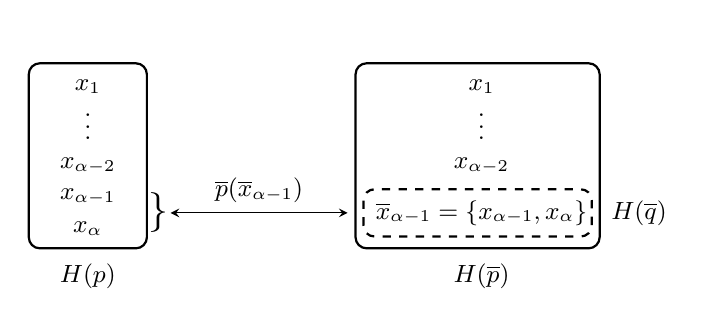
\begin{tikzpicture}
\shorthandoff{>}
%
% Ensemble \A
\draw(0,3) node{\small $\A$};
\draw(0,2.4) node{\small $x_1$};
\draw(0,2) node{\small $\vdots$};
\draw(0,1.4) node{\small $x_{\alpha-2}$};
\draw(0,1) node{\small $x_{\alpha-1}$};
\draw(0,.6) node{\small $x_{\alpha}$};
\draw(0,0) node{\small $H(p)$};
\draw[thick,rounded corners] (-.75,.35) rectangle (.75,2.7);
%
% Ensemble \overline{\A}
%
\draw(5,3) node{\small $\overline{\A}$};
\draw(5,2.4) node{\small $x_1$};
\draw(5,2) node{\small $\vdots$};
\draw(5,1.4) node{\small $x_{\alpha-2}$};
\draw(5,.8) node{\small $\overline{x}_{\alpha-1} = \{x_{\alpha-1} , x_\alpha\}$};
\draw(5,0) node{\small $H(\overline{p})$};
\draw(7,.8) node{\small $H(\overline{q})$};
\draw[dashed,thick,rounded corners] (3.5,.5) rectangle (6.4,1.1);
\draw[thick,rounded corners] (3.4,.35) rectangle (6.5,2.7);
%
% juntando 2 estados VER PROBLEMA CON LA FLECHA
\draw(.9,.8) node{\Large $\}$};
\draw[>=stealth,<->] (1.05,.8)--(3.3,.8);
\draw (2.175,.8) node[above]{\small $\overline{p}(\overline{x}_{\alpha-1})$};
\end{tikzpicture} \end{center}
  %
  \leyenda{Ilustraci\'on de  la propiedad  de recursividad, que  cuantifica como
    decrece la entropia en un  ensemble cuando se juntan dos estados, vincluando
    la entropia  total, la  entropia despues del  la agrupaci\'on y  la entropia
    interna a los dos estados juntados.}
  \label{fig:SZ:Recursividad}
  \end{figure}
%
\item\label{prop:SZ:concavidad} {\it Concavidad:} La  entropia es concava, en el
  sentido  de que  la entropia  de una  combinaci\'on convexa  de distribuciones
  (mezcla) de probabilidades es siempre major o igual a la combinaci\'on convexa
  de entropias: $$\forall \: \{  \lambda_i \}_{i=1}^n, \quad 0 \le \lambda_i \le
  1,  \quad  \sum_i  \lambda_i  =   1  \quad  \mbox{and  cualquier  conjunto  de
    distribuciones} \quad  \{ p_i  \}_{i=1}^n,$$ $$H\left( \sum_i  \lambda_i p_i
  \right)  \ge  \sum_i \lambda_i  H(p_i)$$  Esta  desigualdad  es conocida  como
  desigualdad de  Jensen.  Es  una consequencia directa  de la convexidad  de la
  funci\'on   $\phi:   u   \mapsto   u   \log   u$,   como   ilustrado   en   la
  figura~\ref{fig:SZ:Concavidad}-(a).    La   figura~\ref{fig:SZ:Concavidad}-(b)
  ilustra como se puede obtener una mezcla de distribuciones de dos probabilidad
  $p_1$  (dado  izquierda)  y  $p_2$  (dado  derecho)  haciendo  una  elecci\'on
  aleatoria a  partir de una moneda  en este ejemplo  (probabilidad $\lambda$ de
  elegir   el   dado   izquierda).\newline
  %
  \begin{figure}[h!]
  \begin{center} \begin{tikzpicture}
\shorthandoff{>}
%
% Concavidad de - u log u
\begin{scope}[xscale=3,yscale=2.5]
\pgfmathsetmacro{\u}{.2};
\pgfmathsetmacro{\v}{1.25};
\pgfmathsetmacro{\l}{.7};
%
\draw[>=stealth,->] (-.5,0)--(1.6,0) node[right]{\small $u$};
\draw[>=stealth,->] (0,-.7)--(0,{1.5*log2(1.5)}) node[above]{\small $\phi(u) = u \log u$};
\draw[thick,domain=.005:1.5,samples=200] (0,0)-- plot (\x,{\x*log2(\x)});
\draw[dashed] (\u,{\u*log2(\u)})--(\v,{\v*log2(\v)});
\draw (\u,0)--(\u,-.05) node[below]{\small $u_1$};
\draw (\v,0)--(\v,-.05) node[below]{\small $u_2$};
%
\draw[dashed] ({\l*\u+(1-\l)*\v},.05) node[above]{\small $\lambda u_1 + (1-\lambda) u_2$}
--({\l*\u+(1-\l)*\v},{(\l*\u+(1-\l)*\v)*log2(\l*\u+(1-\l)*\v)});
%
% l phi(u) + (1-l) phi(v)
\draw[dotted]
({\l*\u+(1-\l)*\v},{\l*\u*log2(\u)+(1-\l)*\v*log2(\v)})--(-.05,{\l*\u*log2(\u)+(1-\l)*\v*log2(\v)})
node[left]{\small $\lambda \phi(u_1) + (1-\lambda) \phi(u_2)$};
%
% phi(l u + (1-l) v)
\draw[dotted]
({\l*\u+(1-\l)*\v},{(\l*\u+(1-\l)*\v)*log2(\l*\u+(1-\l)*\v)})--
(-.05,{(\l*\u+(1-\l)*\v)*log2(\l*\u+(1-\l)*\v)})
node[left]{\small $\phi(\lambda u_1 + (1-\lambda) u_2)$};
\end{scope}
%
%
% Concavidad / mezcla
\begin{scope}[xshift=8.5cm]
\draw(0,1.25) node{\includegraphics[width=3cm]{TIKZ_SZ/DosDados}};
\draw(-.5,2.5) node{\small $p_1$};
\draw(1,2) node{\small $p_2$};
\draw(2.7,1) node{\small $\lambda p_1 + (1-\lambda) p_2$};
\draw(-.25,-1) node{\includegraphics[width=1cm]{TIKZ_SZ/Moneda}};
\draw[>=stealth,->,thick] (-.3,-.35)--(-.75,.45);
\draw (-.525,0) node[left]{\small $\lambda$};
\draw[>=stealth,->,thick] (-.2,-.35)--(.3,.45);
\draw (.05,0) node[right]{\small $1-\lambda$};
\end{scope}
%
\draw (1.25,-2.25) node{(a)};
\draw (8.25,-2.25) node{(b)};
\end{tikzpicture} \end{center}
  %
  \leyenda{(a) $\phi(u)  = u \log u$ es  concava: la curva es  siempre debajo de
    sus cuerdas; entonces, cada promedio de $\phi(u_1)$ y $\phi(u_2)$ estando en
    la cuerda  juntando estos punto, queda  arriba de la funci\'on  tomada en el
    promedio de $u_1$  y $u_2$.  Escribiendo eso para (mas  de dos puntos) sobre
    los $\sum_i \lambda_i  p_i(x)$ y sumando sobre los $x$  da la desigualdad de
    Jensen.  (b) Ilustraci\'on de  una distribuci\'on de mezcla, ac\'a mezclando
    $p_1$  y  $p_2$  a  partir  de  una tercera  variable  aleatoria  (ac\'a  de
    Bernoulli).}
  \label{fig:SZ:Concavidad}
  \end{figure}
%
\item\label{prop:SZ:Schurconcavidad}  {\it Schur-concavidad:}  Como se  lo puede
  querrer,  lo mas  ``concentrado'' es  una distribuci\'on  de  probabilidad, lo
  menos hay  incerteza, y entonces lo  mas peque\~no debe ser  la entropia. Esta
  propiedad intuitiva se resuma a partir de la noci\'on de mayorizaci\'on:
  %
  \begin{definicion}[Mayorizaci\'on]\label{def:SZ:Mayorizacion}
    Una distribuci\'on  discreta finita de probabilidad $p$  es dicha mayorizada
    por una distribuci\'on $q$, $$p  \prec q \quad \mbox{ssi} \quad \sum_{i=1}^k
    p^\downarrow(x_i) \le \sum_{i=1}^k q^\downarrow(x_i), \quad 1 \le k < \alpha
    \quad \mbox{y} \quad \sum_{i=1}^\alpha p^\downarrow(x_i) = \sum_{i=1}^\alpha
    q^\downarrow(x_i)$$  (las  \'ultimas  sumas  siendo  igual  a  1).   Si  los
    alfabetos de definici\'on de $p$ y $q$ son de tama\~nos diferentes, $\alpha$
    es el  tama\~no lo mas grande y  la distribuci\'on sobre el  alfabeto lo mas
    corto es completada por estados de  probabilidad 0 (recuerdense de que no va
    a cambiar la entropia).
  \end{definicion}
  %
  La  Schur-concavidad  se  traduce  por  la  relaci\'on  $$  p  \prec  q  \quad
  \Rightarrow \quad  H(p) \ge H(q)$$ Fijense  de que las cotas  sobre $H$ pueden
  ser  vistas como  consecuencia de  esta desiguldad:  la  distribuci\'on cierta
  mayoriza  cualquier  distribuci\'on  y  cualquier distribuci\'on  mayoriza  la
  distribuci\'on uniforme.
\end{propiedades}

En muchos  casos, uno tiene que  trabajar con varias  variables aleatorias. Para
simplificar les  notaciones, considera una par  de variables $X$  y $Y$ definida
respectivamente sobre  los alfabetos $\A$ y  $\B$ de cardinal $\alpha  = |\A|$ y
$\beta = |\B|$.   Tal par de variable puede ser vista  como una variable $(X,Y)$
definida sobre el alfabeto $\A \times  \B$ de cardinal $\alpha \beta$ tal que se
definie naturalmente  la entropia  para esta variable;  tal entropia  es llamada
{\it entropia conjunta} de $X$ y $Y$:
%
%~\cite{Sha48, ShaWea64}
\begin{definicion}[Entropia conjunta]\label{def:SZ:EntropiaConjunta}
  Sean $X$ y $Y$ dos variable aleatorias definidas sobre los alpfabetos discretos
  $\A$  y $\B$,  de  cardinal  $\alpha =  |\A|  < +\infty$  y  $\beta  = |\B|  <
  +\infty$. Sea $p_{X,Y}(x,y)$ la distribuci\'on de probabilidad conjunta de $X$
  e $Y$, \ie $  \forall \, (x,y) \in \A \times \B,  \quad p_{X,Y}(x,y) = \Pr[X =
  x, Y  = y]$. La  entropia conjunta de  Shannon de las  variables $X$ y  $Y$ es
  definida por
  %
  \begin{equation}
  H(p_{X,Y}) = H(X,Y) = - \sum_{(x,y) \in \A \times \B} p_{X,Y}(x,y) \, \log p_{X,Y}(x,y)
  \end{equation}
  %
  con la convenci\'on $0 \log 0 = 0$.
\end{definicion}

A partir de esta definici\'on,  aparecen otras propiedades importantes, sino que
fundamentales, de la entropia de Shannon.
%
\begin{propiedades}
\item\label{prop:SZ:aditividad}  {\it Aditividad:} La  entropia conjunta  de dos
  variables  aleatorias   $X$  e  $Y$  \underline{independientes}   se  suma,  y
  reciprocamente:  $$X   \:  \mbox{e}   \:  Y  \:   \mbox{independientes}  \quad
  \Leftrightarrow \quad  H(X,Y) = H(X) +  H(Y)$$ Dicho de otra  manera, para dos
  variables aleatorias, la incerteza global es la suma de las incertezas de cada
  variable individual.   La propiedad ``$\Rightarrow$''  es consecuencia directa
  de $p_{X,Y}(x,y) = p_X(x) p_Y(y)$. Se va a probar en la secci\'on siguiente la
  reciproca. Se  generaliza sencillamente a un conjunto  de variables aleatorias
  $\{ X_i \}$.
%
\item\label{prop:SZ:subaditividad} {\it Sub-aditividad:} La entropia conjunta de
  dos variables aleatorias  $\{ X_i \}_{i=1}^n$ es siempre menor  que la suma de
  cada entropia individual: $$ H(X_1,\ldots,X_n) \, \le \, \sum_{i=1}^n H(X_i)$$
  Dicho de otra manera, variables  pueden compartir informaci\'on, de tal manera
  de que le entropia global sea menor que la suma.  De la propiedad anterior, se
  obtiene la igualdad ssi los $X_i$ son indepedientes.
%
\item\label{prop:SZ:superaditividad}   {\it   Super-aditividad:}   La   entropia
  conjunta de dos variables aleatorias  $\{ X_i \}_{i=1}^n$ es siempre major que
  cualquiera  de  las entropias  individuales  $$  H(X_1,\ldots,X_n)  \, \ge  \,
  \max_{1 \le i \le n} H(X_i)$$.
\end{propiedades}

Es importante notar  de que existen varios enfoques basados  sobre una series de
axiomas, dando lugar  a la definici\'on de la entropia  tal como definido. Estos
axiomas  son conocidos  como axiomas  de Shannon-Khinchin  y son  la continuidad
(propiedad~\ref{prop:SZ:continuidad}),               la              maximalidad
(propiedad~\ref{prop:SZ:cotamaxima}),              la             expansabilidad
(propiedad~\ref{prop:SZ:expansabilidad})         y         la         aditividad
(propiedad~\ref{prop:SZ:aditividad}).  Existen varios otros conjunto de axiomas,
conduciendo tambi\'en a la entropia de Shannon (ver Shannon~\cite[Sec.~6]{Sha48}
or  \cite{ShaWea64},  R\'enyi~\cite{Ren61}  o Fadeev~\cite{Fad56,  Fad58}  entre
otros).

Para  una  serie de  variables  aleatorias,  $X_1,  X_2, \ldots$,  representando
simbolos, se puede  definir una entropia por simbolo  como una entropia conjunta
divido por numero de simbolos, $\frac{H(X_1,\ldots,x_n)}{n}$, as\'a que una taza
de entropia cuando $n$ va al inifinito.
%
\begin{definicion}[Taza de entropia]\label{def:SZ:TazaDeEntropia}
  Sea $\X = \{  X_i \}_{i \in \Nset^*}$ una  serie de variable aleatoria.  La taza de
  entropia de esta serie es definida por
  %
  \begin{equation}
  \H(\X) = \lim_{n \to \infty} \frac{H(X_1,\ldots,X_n)}{n}
  \end{equation}
  %
\end{definicion}
%
\noindent Esta cantidad siempre existe, porque $H(X_1 , \ldots , X_n) \le \sum_i
H(X_i) \le \sum_i \log \alpha_i \le  n \max_i \alpha_i$ donde los $\alpha_i$ son
los cardinales de los alfabetos de definici\'on de los $X_i$.

\

Se termina esta sub-secci\'on con el caso de variables discretas definidas sobre
un  alfabeto $\A$ de  cardinal infinito  $|\A| =  + \infty$,  por ejemplo  $\A :
\Nset$.   Por  analogia,  se  puede  siempre  definir la  entropia  como  en  la
definici\'on Def.~\ref{def:SZ:Shannon}. Esta extensi\'on resuelta delicada dando
de que unas  propiedades se perdien.  Por ejemplo, la  entropia no queda acotada
por  arriba como  se  lo puede  probar  para la  distribuci\'on de  probabilidad
$\displaystyle p(x)  \propto \frac{1}{(x+2) \left(  \log (x+2) \right)^2},  \: x
\in \Nset$,  corectamente normalizada ($\propto$  significa ``proporcional a''):
$\displaystyle \frac{\log \log(x+2)}{(x+2) \left( \log (x+2) \right)^2} \ge 0$ y
la serie $\displaystyle \sum_x  \frac{1}{(x+2) \log (x+2)}$ es divergente, as\'i
que la serie $\displaystyle - \sum_x p(x) \log p(x)$ diverge.

% ================================= Axiomas

\subseccion{Entrop\'ia diferencial}
\label{ss:SZ:Diferencial}

Volviendo a la definici\'on Def.~\ref{def:SZ:Shannon} de la entropia de Shannon,
usando el operador $\Esp$ promedio  estadistica o esperanza matematica, se puede
rescribir la entropia de Shannon como $H(X) = \Esp\left[ - \log p_X(X) \right]$.
Con este punto  de vista, es facil extender la definici\'on  de la entropia para
variables aleatorias continuas admitiendo  una densidad de probabilidad.  Eso da
lugar a lo que es conocido como la {\it entropia diferencial}:

\begin{definicion}[Entropia diferencial]\label{def:SZ:EntropiaDiferencial}
  Sea $X$ una  variable aleatoria definida sobre un  espacio $d$-dimensional $\D
  \subseteq \Rset^d$ y sea $p_X(x)$ la densidad (distribuci\'on) de probabilidad
  de $X$, La entropia diferencial de la variable $X$ es definida por
  %
  \begin{equation}
    H(p_X) = H(X) = - \int_{\D} p_X(x) \, \log p_X(x) \, dx
  \end{equation}
  %
  (con la  convenci\'on $0 \log  0 = 0$,  se puede escribir la  integraci\'on en
  $\Rset^d$).
\end{definicion}
%
Como en el  caso discreto, para $X = (X_1,\ldots,X_d)$, esta  entropia de $X$ es
dicha entropia conjunta de los componentes $X_i$.

Como se lo  va a ver, la entropia diferencial no  tiene la misma significaci\'on
de  incerteza,  siendo de  que  depende no  solamente  de  la distribuci\'on  de
probabilidad, sino  que de los estados tambi\'en.  Mas alla, no se  la puede ver
como l\'imite continua de un caso discreto:  a trav\'es de tal l\'imite, se va a
ver que se  llama diferencial, a causa del efecto de  la diferencial $dx$.  Para
ilustrar  eso,  considera una  variable  aleatoria  escalar  $X$ viviendo  sobre
$\Rset$ y $p_X$ su densidad de probabilidad.  Sea $\delta > 0$ y sea el alfabeto
$\A^\delta  = \{  x_k  \}_{k \in  \Zset}$ donde  los  $x_k$ se  definen tal  que
$\displaystyle p_X(x_k)  \delta = \int_{k \delta}^{(k+1) \delta}  p_X(x) \, dx$,
como ilustrado en la figure~\ref{fig:SZ:CuantificacionX}.  Se define la variable
aleatoria discreta $X^\delta$  sobre $\A^\delta$ tal que $\Pr[X^\delta  = x_k] =
p_{X^\delta}(x_k) = p_X(x_k) \delta$. Se  puede ver $X^\delta$ como la versi\'on
cuantificada de $X$, con $X^\delta = x_k$ cuando $X \in [k \delta , (k+1) \delta
)$.   Al rev\'es,  a\'un que  sea  delicado, se  puede interpretar  $X$ como  el
``l\'imite'' de $X^\delta$ cuando $\delta$ tiende a 0. Ahora, es claro de que
%
\begin{eqnarray*}
H(X^\delta) & = & - \sum_k p_{X^\delta}(x_k) \log p_{X^\delta}(x_k)\\[2.5mm]
%
& = & - \log \delta - \sum_k \Big( p_X(x_k) \log p_X(x_k) \Big) \, \delta
\end{eqnarray*}
%
lo que se escribe tambien $$H(X^\delta)  + \log \delta = - \sum_k \Big( p_X(x_k)
\log p_X(x_k)  \Big) \, \delta$$ Entonces,  de la intergraci\'on  de Rieman sale
que
%
\begin{equation*}
\lim_{\delta \to 0} \left( H(X^\delta) + \log \delta \right) = H(X)
\end{equation*}
%
Dicho de  otra manera,  la entropia  diferencial de $X$  no es  el limite  de la
entropia  de su  versi\'on  cuantificada:  aparece con  la  entropia el  termino
``diferencial'' $\log \delta$.
%
\begin{figure}[h!]
\begin{center} 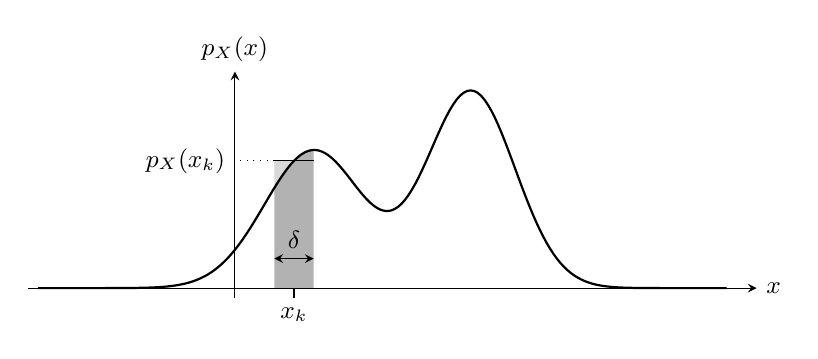
\begin{tikzpicture}
\shorthandoff{>}
%
% Cuantificacion de X
\begin{scope}[xscale=2.5,yscale=2.5]
%
\pgfmathsetmacro{\c}{.4};
\pgfmathsetmacro{\d}{1.2};
\pgfmathsetmacro{\s}{8};
\pgfmathsetmacro{\t}{10};
\pgfmathsetmacro{\a}{.7};
\pgfmathsetmacro{\b}{1};
%
\pgfmathsetmacro{\xk}{.3};
\pgfmathsetmacro{\dx}{.2};
%
\draw[>=stealth,->] (-1.05,0)--(2.65,0) node[right]{\small $x$};
\draw[>=stealth,->] (0,-.05)--(0,1.1) node[above]{\small $p_X(x)$};
%
% lei de proba
\draw[thick,domain=-1:2.5,samples=200] plot (\x,{(\a*exp(-\s*(\x-\c)^2)+\b*exp(-\t*(\x-\d)^2))});
%
% dominio alrededor de xk
\fill[domain=\xk-\dx/2:\xk+\dx/2,samples=20,opacity=.3]
({\xk-\dx/2},0)--
plot (\x,{(\a*exp(-\s*(\x-\c)^2)+\b*exp(-\t*(\x-\d)^2))})--
({\xk+\dx/2},0);
%
% xk y delta
\draw (\xk,0)--(\xk,-.05) node[below]{\small $x_k$};
\draw[>=stealth,<->] ({\xk-\dx/2},.15)--({\xk+\dx/2},.15);
\draw (\xk,.15) node[above]{\small $\delta$};
%
% recta sobre delta a altura de p(xk)
\draw ({\xk+\dx/2},{(\a*exp(-\s*(\xk-\c)^2)+\b*exp(-\t*(\xk-\d)^2))})--
({\xk-\dx/2},{(\a*exp(-\s*(\xk-\c)^2)+\b*exp(-\t*(\xk-\d)^2))});
\draw[dotted] ({\xk-\dx/2},{(\a*exp(-\s*(\xk-\c)^2)+\b*exp(-\t*(\xk-\d)^2))})--
(0,{(\a*exp(-\s*(\xk-\c)^2)+\b*exp(-\t*(\xk-\d)^2))}) node[left]{\small $p_X(x_k)$};
%
% dominio equivalente alrededo de xk
\fill[domain=\xk-\dx/2:\xk,samples=20,opacity=.15]
plot (\x,{(\a*exp(-\s*(\x-\c)^2)+\b*exp(-\t*(\x-\d)^2))})--
({\xk-\dx/2},{(\a*exp(-\s*(\xk-\c)^2)+\b*exp(-\t*(\xk-\d)^2))});
\end{scope}
\end{tikzpicture} \end{center}
%
\leyenda{Densidad de probabilidad $p_X$ de $X$, construcci\'on del alfabeto $\A$
  donde  se  define   la  versi\'on  cuantificada  $X^\delta$  de   $X$  con  su
  distribuci\'on discreta de probabilidad $p_{X^\delta}$. La superficia en grise
  oscuro es igual a la superficia definida por el rectangulo en grise claro.}
\label{fig:SZ:CuantificacionX}
\end{figure}
%

Mas  all\'a  de  esta  notable  diferencia  entre  la  entropia  y  la  entropia
diferencial, la \'ultima depende de los estados,  es decir que si $Y = g(X)$ con
$g$  biyectiva,  no  se  conserva  la  entropia,  \ie  \underline{se  pierde  la
  propiedad~\ref{prop:SZ:biyeccion}}  del  caso discreto:
%
\begin{eqnarray*}
H(Y) & = & - \int_{\Rset^d} p_Y(y) \log p_Y(y) \, dy\\[2.5mm]
%
& = &  - \int_{\Rset^d} p_Y(g(x)) \log p_Y(g(x)) \, |\Jac_g(x)| \, dx\\[2.5mm]
%
& = & - \int_{\Rset^d} p_Y(g(x)) \Big( \log \big( p_Y(g(x)) \, |\Jac_g(x)| \big) -
\log |\nabla^t g(x)| \Big) \, |\Jac_g(x)| \, dx
\end{eqnarray*}
%
donde $\Jac_g$ es la  matriz de componentes $\frac{\partial g_i}{\partial x_j}$,
Jacobiano  de  la transformaci\'on  $g:  \Rset^d  \mapsto  \Rset^d$ y  $|\cdot|$
representa el valor absoluto del determinente de la matriz.  Recordandose de que
$p_X(x) = p_Y(g(x)) |\Jac_g(x)|$, se obtiene
%
\begin{propiedadesC}\setcounter{enumi}{\value{PropBiyeccion}}
%
\item\label{prop:SZ:biyeccionC}
Para cualquier biyecci\'on $g: \Rset^d \mapsto \Rset^d$
  \begin{equation*}
    H(g(X)) = H(X) +  \int_{\Rset^d} p_X(x) \log |\Jac_g(x)| \, dx
  \end{equation*}
  %
  donde el \'ultimo termino, $\Esp\left[  \log |\Jac_g(X)| \right]$ no vale cero
  en    general.   En    particular,   si    $H$   es    invariante    bajo   un
  deplazamiento,  $$H(X+\mu) = H(X)  \quad \forall  \: \mu  \in \Rset^d$$  no es
  invariante por cambio de escala, $$H(a X) = H(X) + \log |a| \quad \forall \: a
  \in \Rset^*$$
\end{propiedadesC}
%
Esta  \'ultima relaci\'on  queda valid  para  $a$ matriz  invertible.  Por  esta
\'ultima  relaci\'on, se puede  ver que,  dado $X$,  cuando $a$  tiende a  0, la
entropia de  $a X$ tiende a  $-\infty$.  Es decir que,  para $a$ suficientemente
peque\~no,  se  puede  tener $H(a  X)  <  0$,  as\'i que  \underline{se  pierde}
tambi\'en \underline{la positividad, propiedad~\ref{prop:SZ:positividad}}.  Esta
perdida definitivamente quita la interpretaci\'on de incerteza/informaci\'on que
hubiera podido tener la entropia diferencial.  A veces, se usa lo que es llamado
potencia entropica:
%
\begin{definicion}[Potencia entropica]
  Sea $X$ una  variable aleatoria $d$-dimensional. La potencia  entropica de $X$
  es definida por $$N(X) = \frac{2 \pi \e} \exp\left( \frac2d H(X)
  \right)$$
\end{definicion}
%
\noindent Por construcci\'on,  $N(X) \ge 0$.  Ademas, en  el caso continuo, $N(a
X+b) = |a|^2 N(X)$ (queda valida para una matriz $a$ invertible): esta propiedad
puede justificar la idea de  ``potencia''; ademas $N(a X+b)$ tiende naturalmente
a cero cuando $a$ tiende a  cero.  Se recupera as\'i la noci\'on informacional a
trav\'es  de  $N$ en  este  contexto  ($a X  +  b$  ``tiende''  a $b$,  variable
deterministica).

Si se pierde  la propiedad de invarianza bajo  una biyecci\'on, sopredentemente,
se conserva la entropia bajo el equivalente continuo del rearreglo.
%
\begin{definicion}[Rearreglo simetrico]
  Sea $\P \subset \Rset^d$ abierto de  volumen finito $|\P| < +\infty$.  El {\it
    rearreglo simetrico}  $\P^\downarrow$ de  $\P$ es la  bola centrada en  0 de
  mismo volumen  que $\P$, \ie $$\P^\downarrow =  \left\{ x \in \Rset^d  \, : \:
    \frac{2  \pi^{\frac{d}{2}}  |x|^d}{\Gamma\left(\frac{d}{2}\right)} \le  |\P|
  \right\}$$  donde $|\cdot|$  denota  la norma  euclideana.   Eso es  ilustrado
  figure~\ref{fig:SZ:ensemblerearreglado}-a.\newline  Sea $p_X$ una  densidad de
  probabilidad y sea $\P_t = \{ y \, : \: p_X(y) > t \}$ para cualquier $t > 0$,
  sus ensembles  de niveles.  La densidad de  probabilidad~\footnote{Se proba de
    que  esta funci\'on,  positiva  por  definici\'on, suma  a  1.  Ademas,  por
    construcci\'on,  depende   unicamente  de   $|x|$  y  decrece   con  $|x|$.}
  rearreglada    simetrica    $p^\downarrow_X$     de    $p_X$    es    definida
  por  $$p^\downarrow_X(x) =  \int_0^{+\infty} \un_{\P_u^\downarrow}(x)  \, du$$
  con $\un_A$ el indicator  del ensemble $A$, \ie $\un_A(x) = 1$  si $x \in A$ y
  cero sino.
\end{definicion}
%
Del hecho  de que $\forall \, t  < \tau \: \Leftrightarrow  \: \P_\tau \subseteq
\P_t  \:  \Leftrightarrow \:  \P_\tau^\downarrow  \subseteq \P_t^\downarrow$  es
sencillo   ver   que   si   $x   \in  \P_\tau^\downarrow$,   entonces   $x   \in
\P_t^\downarrow$, lo que conduce a  $p_X^\downarrow(x) > \tau$ y vice-versa. Mas
alla,  sobre $\P_{\tau+d\tau}  \backslash \P_\tau$  la funci\'on  $p_X$ ``vale''
$\tau$ \ y \ sobre $\P_{\tau+d\tau}^\downarrow \backslash \P_\tau^\downarrow$ la
funci\'on $p_X^\downarrow$  ``vale'' tambien $\tau$, lo que  da \ $\displaystyle
\int_{\P_\tau^\downarrow} p_X^\downarrow(x) \, dx = \int_{\P_\tau} p_X(x) \, dx$
(ver~\cite{LieLos01, WanMad04} para une prueba mas rigorosa).  La representaci\'on de la
definici\'on es conocida como representaci\'on en capas de pastel (layer cake en
ingles). Eso es ilustrado en la figura~\ref{fig:SZ:ensemblerearreglado}-b
  %
  \begin{figure}[h!]
  \begin{center} 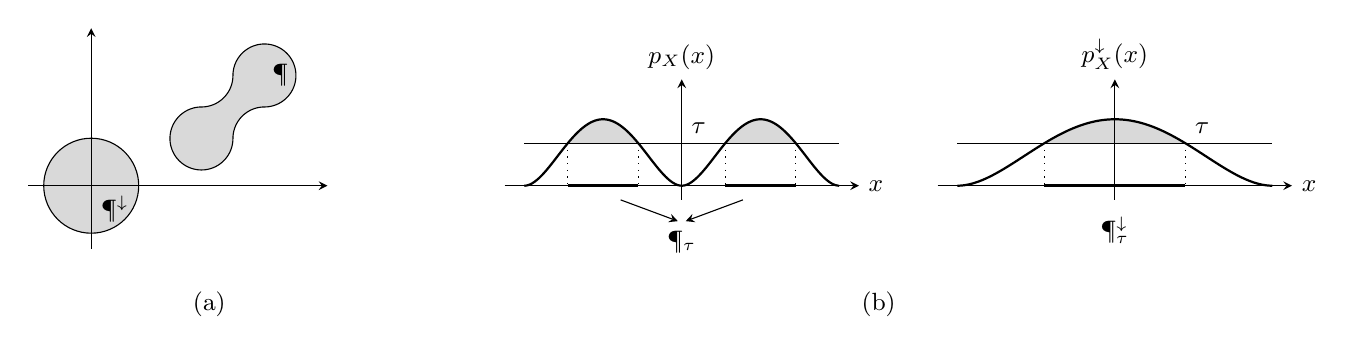
\begin{tikzpicture}
\shorthandoff{>}
%
\begin{scope}[scale=.4]
% Superficia 2*3 pi/4  + 2*2 - 2*pi/4 = 4+pi
\filldraw[draw=black,fill=gray!30]
   plot [domain=0:-270,samples=200] ({cos(\x)+3.5},{sin(\x)+1.5})
-- plot [domain=-90:0,samples=200] ({cos(\x)+3.5},{sin(\x)+3.5})
-- plot [domain=180:-90,samples=200] ({cos(\x)+5.5},{sin(\x)+3.5})
-- plot [domain=90:180,samples=200] ({cos(\x)+5.5},{sin(\x)+1.5})
-- cycle;
\draw (6,3.5) node {\small $\P$};
%
% superficia rearreglada
\filldraw[draw=black,fill=gray!30] (0,0) circle ({sqrt(1+4/pi)});
\draw (.75,-.75) node {\small $\P^\downarrow$};
%
% ejes
\draw[>=stealth,->] (-2,0)--(7.5,0);
\draw[>=stealth,->] (0,-2)--(0,5);
%
\end{scope}
%
%
%----------------------------------------
%
% p_X(x), P_tau...
\begin{scope}[xshift=7.5cm,yscale=1.8]
\pgfmathsetmacro{\t}{.3};
\pgfmathsetmacro{\xt}{sqrt(1-sqrt(32*\t/15))};
\pgfmathsetmacro{\dx}{5.5};% shift para p*(x)
\pgfmathdeclarefunction{studr}{1}{\pgfmathparse{(15/32)*((1-(#1)^2)^2)}}; %Student-r
%
% mezcla de Student-r 15/16 * (1-x^2)^2 (nu = 5) centrados en -1 y 1
% 15/32 (1-(x-a)^2)^2 > t iif (x-a)^2 < 1-sqrt(32*t/15)
% i.e. a-sqrt(1-sqrt(32*t/15)) < x < a+sqrt(1-sqrt(32*t/15))
\fill[domain=-1-\xt:-1+\xt,fill=gray!30] plot(\x,{studr(\x+1)}); % p(x) > tau, x < 0
\fill[domain=1-\xt:1+\xt,fill=gray!30] plot(\x,{studr(\x-1)}); % p(x) > tau, x > 0
\draw[thick,domain=-2:0,samples=100] plot(\x,{studr(\x+1)}); % p(x), x < 0
\draw[thick,domain=0:2,samples=100] plot(\x,{studr(\x-1)}); % p(x), x > 0
\draw (-2,\t)--(2,\t); \draw (0,\t) node[above right]{\small $\tau$}; % y = tau
%
% dominio P_tau
\draw[dotted] ({-1-\xt},{studr(\xt)})--({-1-\xt},0);
\draw[dotted] ({-1+\xt},{studr(\xt)})--({-1+\xt},0);
\draw[very thick] ({-1-\xt},0)--({-1+\xt},0);
\draw[>=stealth,->] ({-1+\xt/2},-.1)--(-.05,-.25);
%
\draw[dotted] ({1-\xt},{studr(\xt)})--({1-\xt},0);
\draw[dotted] ({1+\xt},{studr(\xt)})--({1+\xt},0);
\draw[very thick] ({1-\xt},0)--({1+\xt},0);
\draw[>=stealth,->] ({1-\xt/2},-.1)--(.05,-.25);
%
\draw (0,-.25) node[below]{\small $\P_\tau$};
%
% ejes
\draw[>=stealth,->] (-2.25,0)--(2.25,0) node[right]{\small $x$};
\draw[>=stealth,->] (0,-.1)--(0,.75) node[above]{\small $p_X(x)$};
%
%---------------------------
%
% 15/32 (1-(x-a)^2)^2 > t iif (x-a)^2 < 1-sqrt(32*t/15)
% i.e. a-sqrt(1-sqrt(32*t/15)) < x < a+sqrt(1-sqrt(32*t/15))
% Volumen 2*sqrt(1-sqrt(32*t/15))
% Por simetria, P_t* = [-2*sqrt(1-sqrt(32*t/15)) , 2*sqrt(1-sqrt(32*t/15))]
% da f*(x) = 15/32 (1-x^2/4)^2
\fill[domain=-2*\xt:2*\xt,fill=gray!30] plot({\x+\dx},{studr(.5*\x)}); % p*(x) > tau
\draw[thick,domain=-2:2,samples=200] plot({\x+\dx},{studr(.5*\x)});
\draw ({-2+\dx},\t)--({2+\dx},\t); \draw ({2*\xt+\dx},\t) node[above right]{\small $\tau$}; % y = tau
%
% dominio P_tau*
\draw[dotted] ({-2*\xt+\dx},{studr(\xt)})--({-2*\xt+\dx},0);
\draw[dotted] ({2*\xt+\dx},{studr(\xt)})--({2*\xt+\dx},0);
\draw[very thick] ({-2*\xt+\dx},0)--({2*\xt+\dx},0);
%
\draw (\dx,-.15) node[below]{\small $\P_\tau^\downarrow$};
%
% ejes
\draw[>=stealth,->] ({-2.25+\dx},0)--({2.25+\dx},0) node[right]{\small $x$};
\draw[>=stealth,->] (\dx,-.1)--(\dx,.75) node[above]{\small $p_X^\downarrow(x)$};
\end{scope}
%
\draw (1.5,-1.5) node{\small (a)};
\draw (10,-1.5) node{\small (b)};
\end{tikzpicture} \end{center}
  %
  \leyenda{(a):  Ilustraci\'on  del rearreglo  simetrico  $\P^\downarrow$ de  un
    ensemble  $\P$,  siendo  la  bola  centrada  en  0  de  mismo  volumen.  (b)
    Construcci\'on  del rearreglo  $p_X^\downarrow$:  dado un  $\tau$, se  busca
    $\P_\tau$ y  se deduce $P_\tau^\downarrow$; dado  un $x$, se  busca el mayor
    $t$  tal  que  $x  \in  P_t^\downarrow$, este  $t$  maximo  siendo  entonces
    $p_X^\downarrow(x)$;  ademas, por construcci\'on,  las superficias  en grise
    son iguales.}
  \label{fig:SZ:ensemblerearreglado}
  \end{figure}
% =  \B  \left( 0  , r_\P  \right)$ con  $\frac{2
%    \pi^{d/2} r_\P^d}{\Gamma(d/2)} = |\P|$.

\begin{propiedadesC}\setcounter{enumi}{\value{PropPermutacion}}
\item\label{prop:SZ:permutacionC} {\it invarianza  bajo un rearreglo:} Sea $p_X$
  densidad   de  probabilidad   sobre   un  abierto   de  $\Rset^d$,   $$H\left(
    p_X^\downarrow \right) = H(p_X)$$
\end{propiedadesC}
%
\noindent Esta propiedad es probada por ejemplo en~\cite{LieLos01, WanMad04}.

{\color{red}\bf      a      ver       que      pasa      en      termino      de
  mayorizacion~\ref{prop:SZ:mayorizacion}?}

Como  se lo  ha visto,  la  entropia diferencial  no es  siempre positiva,  como
consecuencia  de~\ref{prop:SZ:biyeccionC}.   Tambi\'en,  la  propiedad  de  cota
superior,  \underline{propiedad~\ref{prop:SZ:cotamaxima} se pierde}  en general,
\underline{salvo si se pone vinculos}:
%
\begin{propiedadesC}\setcounter{enumi}{\value{PropCotamaxima}}
\item
\begin{enumerate}
\item\label{prop:SZ:cotamaximauniforme} Si  $\D$ es de volumen finito  $|\D| < +
  \infty$,  la  entropia es  acotada  por arriba,  $$H(X)  \le  \log |\D|$$  con
  igualdad ssi $X$ es \underline{uniforme}.
%
\item\label{prop:SZ:cotamaximagaussiana} Si $\D =\Rset^d$ y $X$ tiene una matriz
  de  covarianza dada  $\Sigma_X =  \Esp\left[  X X^t  \right]$ donde  $\cdot^t$
  denota la transpuesta, la entropia es tambi\'en acotada por arriba, $$H(X) \le
  \frac{d}{2} \log(2 \pi \e) + \frac12 \log |\Sigma_X|$$ con igualdad ssi $X$ es
  \underline{gaussiana}.  En  particular, la potencia entropica  de la gaussiana
  vale $N(X) = |\Sigma_X|^{\frac1d}$, dando  de nuevo un ``sabor'' de potencia a
  $N$. Como se o va a ver  en este cap\'itulo, la gaussiana juega un rol central
  en la teoria de la informaci\'on.
\end{enumerate}
\end{propiedadesC}
%
{\bf\color{red} Poner MaxEnt mas general? Con vinculo tipo desigualdad de Gibbs,
  o momentos y leyes de la familia exponencial?}

Al      final,     \underline{se      conservan      las     propiedades      de
  concavidad~\ref{prop:SZ:concavidad},  de aditividad~\ref{prop:SZ:aditividad} y
  de sub-aditividad~\ref{prop:SZ:subaditividad}}.   Es interesante de  notar que
de  la desigualdad~\ref{prop:SZ:subaditividad},  puramente  entropica, se  puede
deducir la  desigualdad de Hadamard,  desigualdad puramente matricial:  $|R| \le
\prod_i  R_{i,i}$  para  cualquier  matriz simetrica  definida  positiva  (viene
de~\ref{prop:SZ:subaditividad} escrita  para una  gaussiana de covarianza  $R$ y
tomando una exponencial de la desigualdad).


% ================================== Mutua =================================== %

\seccion{Entropia condicional, informaci\'on mutua, entropia relativa}
\label{s:SZ:Mutua}

Tratando de un par de variable  aleatorias $X$ e $Y$, una cuesti\'on natural que
occure es de cuantificar la incerteza que queda sobre una de las variable cuando
se  observa  la  otra.  Dicho  de  otra  manera, si  se  mide  $Y  =  y$,  ?`que
informaci\'on lleva sobre  $X$? La respuesta a esta  interogaci\'on se encuentra
en la  noci\'on de entropia condicional. Si  uno mide $Y =  y$, la descripci\'on
estadistica de $X$ conociendo este $Y$ se resuma a la distribuci\'on condicional
de  probabilidad $p_{X|Y}  = \frac{p_{X,Y}}{p_Y}$.   Con esta  restricci\'on, se
puede  evaluar una  incerteza sobre  $X$, sabiendo  de que  $Y=y$,  $$H(X|Y=y) =
H\left(  p_{X|Y}(\cdot,y)  \right)$$ Entonces,  condicionalmente  a la  variable
aleatoria $Y$,  la incerteza va  a ser el  promedio estadistico sobre  todos los
estados $Y$ es decir $H(X|Y) = \sum_y p_Y(y) H(X|Y=y)$:
%
\begin{definicion}[Entropia condicional]\label{def:SZ:entropiacondicional}
  Sean $X$ e $Y$ dos  variables aleatorias discretas, la entropia condicional de
  $X$ sabiendo  $Y$ es  definida por $$H(X|Y)  = - \sum_{x,y}  p_{X,Y}(x,y) \log
  p_{X|Y}(x,y)$$
\end{definicion}
%
Esta definici\'on se transpone naturalmente a la entropia diferencial:
%
\begin{definicion}[Entropia diferencial condicional]\label{def:SZ:entropiadiferencialcondicional}
  Sean $X$ e $Y$ dos  variables aleatorias continuas, la entropia condicional de
  $X$ sabiendo $Y$ es definida por $$H(X|Y) = - \int_{\Rset^d} p_{X,Y}(x,y) \log
  p_{X|Y}(x,y) \, dx \, dy$$
\end{definicion}

Si $X$ e $Y$ son indepedientes, $p_{X|Y}$ se reduce a $p_X$, as\'i que vale cero
la entropia condicional:
%
\begin{propiedades}
\item\label{prop:SZ:independenciacondicional}   $$X    \:   \mbox{e}   \:    Y   \:
  \mbox{independientes} \quad \Leftrightarrow \quad H(X|Y) = H(X)$$
\end{propiedades}
%
Esta  propiedad  vale  en ambos  casos,  discreto  como  continuo.  En  el  caso
discreto, se interpreta como el hecho  de que $Y$ no lleva ninguna informaci\'on
sobre $X$, y intonces ninguna medici\'on  de $Y$ va a cambiar la incerteza sobre
$X$.

Siendo $H(X|Y=y)$  una entropia,  va a  heredir de todas  las propiedades  de la
entropia  (diferencial).  Ademas,  de  $p_{X,Y}  = p_{X|Y}  p_Y$  de  deduce  la
propiedad siguiente (valida para la entropia como su extensi\'on diferencial)
%
\begin{propiedades}
\item\label{prop:SZ:cadena}  {\it Regla de  cadena} $$H(X,Y)  = H(X|Y)  + H(Y)$$
  Esta  regla, valida  en ambos  casos,  discreto como  continuo, se  generaliza
  sencillamente a $$H(X_1 , \ldots  , X_n) = H(X_1) + \sum_{i=2}^n H(X_i|X_{i-1}
  ,   \ldots   ,   X_1)$$   De   esta   regla   de   cadena   se   recupera   la
  propiedad~\ref{prop:SZ:independenciacondicional}     a     partir    de     la
  propiedad~\ref{prop:SZ:aditividad}.
\end{propiedades}
%
Siendo  $H(X|Y=y)$  una   entropia,  en  el  caso  discreto   esta  cantidad  es
positiva. Entonces, en  el caso discreto, $H(X|Y)$ es positiva,  lo que proba la
la super-aditividad~\ref{prop:SZ:superaditividad}.

De la regla de  cadena $H(X,Y) = H(X|Y) + H(Y) = H(Y|X)  + H(X)$ aparece que las
cantidades  $H(X|Y)-H(X)$, $H(Y|X)-H(Y)$  y $H(X,Y)  -  H(X) -  H(Y)$ son  todas
iguales. Estas canditades definen lo que se llama la informaci\'on mutua entre \
$X$ \ e \ $Y$:

%
\begin{definicion}[Informaci\'on mutua]\label{def:SZ:mutua}
  Sean $X$ e $Y$ dos variables  aleatorias, la informaci\'on mutua entre \ $X$ \
  e  \ $Y$ \  es la  cantida simetrica  $$I(X;Y) =  H(X|Y)-H(X) =  H(Y|X)-H(Y) =
  H(X,Y) -  H(X) - H(Y)$$ En el  caso discreto se expresa  $$I(X;Y) = \sum_{x,y}
  p_{X,Y}(x,y)  \log \left(  \frac{p_{X,Y}(x,y)}{p_X(x) p_Y(y)}  \right)$$  y su
  forma  diferencial, se  escribe  $$I(X;Y) =  \int_{\Rset^d} p_{X,Y}(x,y)  \log
  \left( \frac{p_{X,Y}(x,y)}{p_X(x) p_Y(y)} \right) \, dx \, dy$$
\end{definicion}

Las diferentes cantitades  peden ser vista a trav\'es  una visi\'on ensemblista,
como  descrita el la  figura~\ref{fig:SZ:Venn}. Este  diagrama es  conocido como
diagrama de Venn.
%
\begin{figure}[h!]
\begin{center} 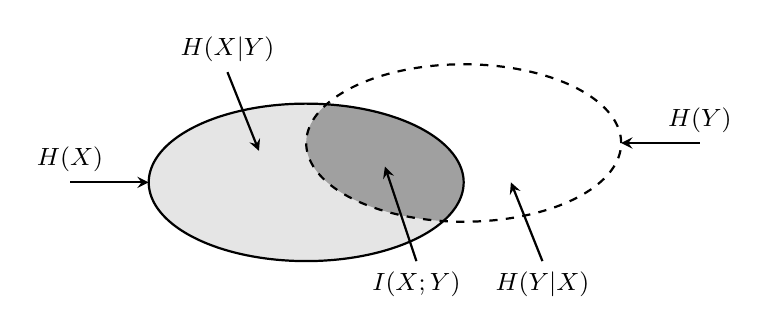
\begin{tikzpicture}[scale=2]
\shorthandoff{>}
% interior H(X) x^2 + 4 y^2 = 1 => y = \pm sqrt(1-x^2)/2
\fill[domain=0:360,samples=200,opacity=.1] plot ({cos(\x)},{.5*sin(\x)});
%
% interior H(Y) (x-1)^2 + 4 (y-1/4)^2 = 1 => y = 1/4 \pm sqrt(1-(x-1)^2)/2
% se cruzan cuando x = 1 \pm sqrt(55)/10 =>
% theta = acos(.5 \pm sqrt(55)/20) para X
% theta = acos(-.5 \pm sqrt(55)/20) para X
\pgfmathsetmacro{\s}{acos(.5-sqrt(55)/20)};
\pgfmathsetmacro{\t}{-acos(.5+sqrt(55)/20)};
\pgfmathsetmacro{\u}{-acos(-.5+sqrt(55)/20)};
\pgfmathsetmacro{\v}{acos(-.5-sqrt(55)/20)-360};
%
% interior I(X;Y)
%\draw[domain=\v:\v] plot ({cos(\x)+1},{.5*sin(\x)+.25}) node{$\bullet$};
\fill[opacity=.3]
   plot [domain=\s:\t,samples=200] ({cos(\x)},{.5*sin(\x)})
-- plot [domain=\u:\v,samples=200] ({cos(\x)+1},{.5*sin(\x)+.25})
-- cycle;
%
% borders H(X) y H(Y)
\draw[domain=0:360,samples=200,thick] plot ({cos(\x)},{.5*sin(\x)});
\draw[dashed,domain=0:360,samples=200,thick] plot ({cos(\x)+1},{.5*sin(\x)+.25});
%
% flechas y flechas condicionales
\draw[thick,>=stealth,<-] (-1,0)--(-1.5,0) node[above]{\small $H(X)$};
\draw[thick,>=stealth,<-] (-.3,.2)--(-.5,.7) node[above]{\small $H(X|Y)$};
%
\draw[thick,>=stealth,<-] (2,.25)--(2.5,.25) node[above]{\small $H(Y)$};
\draw[thick,>=stealth,<-] (1.3,0)--(1.5,-.5) node[below]{\small $H(Y|X)$};
%
\draw[thick,>=stealth,<-] (.5,.1)--(.7,-.5) node[below]{\small $I(X;Y)$};
\end{tikzpicture} \end{center}
\leyenda{Diagrama  de Venn:  Ilustraci\'on  de la  definici\'on  de la  entropia
  condicional,  informaci\'on  mutua, y  los  vinculos  entre  cada medida.   La
  superficia  del elipse en  linea llena  (parte grise)  representa $H(X)$  y el
  interior  de la en  linea punteada  representa $H(Y)$.   La parte  grise clara
  representa  $H(X|Y)$ superficia  del  ensemble $H(X)$  quitando  la parte  que
  partenece  a  $H(Y)$.  La  parte  blanca  representa  $H(Y|X)$ superficia  del
  ensemble $H(Y)$  quitando la parte que  partenece a $H(X)$. La  parte en grise
  oscuro es entonces lo que $X$ e $Y$ comparten, es decir $I(X;Y)$.}
\label{fig:SZ:Venn}
\end{figure}

Como se lo va a probar, $I$ es positiva; representa realmente una informaci\'on,
la compartida  entre \ $X$  \ e  \ $Y$. Si  de la incerteza  de $X$ se  quita la
incerteza  de  $X$   una  vez  que  $Y$  es  medida,  lo   que  queda  tiene  la
significaci\'on de la informaci\'on que  estas variables tienen en com\'un. Para
probar la positividad de $I$, se  introduce de manera mas general la noci\'on de
entropia     relativa,     conocida     tambi\'en    como     divergencia     de
Kullback-Leibler~\cite{CovTho06, Rio07, Kul}:
%
{\bf\color{red} Buscar ref de Kullback and so on}
%
\begin{definicion}[Entropia relativa]\label{def:SZ:entropiarelativa}
  La entropia relativa, o divergencia de una distribuci\'on de probabilidad $q$,
  con  respeco a  una distribuci\'on  de referencia  $p$, donde  el  alfabeto de
  definici\'on de $p$ inluye lo de $q$, es definida como $$D(q\|p) = \sum_x q(x)
  \log \left( \frac{q(x)}{p(x)} \right)$$ o, en su forma diferencial $$D(q\|p) =
  \int_{\Rset^d} q(x) \log \left( \frac{q(x)}{p(x)} \right) \, dx$$
\end{definicion}
%
Esta  medida se  puede ser  vista como  una entropia  de la  distribuci\'on $q$,
relativamente a  una distribuci\'on de referencia  $p$. Por ejemplo,  en el caso
discreto  finito, si  $p$ es  la distribuci\'on  uniforme sobre  un  alfabeto de
cardinal  $\alpha$,  $D(q\|p) =  \log  \alpha -  H(q)$,  lo  que representa  una
desviaci\'on  de la  entropia con  su valor  maximal. La  misma interpretaci\'on
queda en  el caso continuo  con la  lei uniforme ($p$  y $q$ definidas  sobre el
mismo espacio  de volumen finito) o  con la gaussiana  ($p$ y $q$ dando  la misma
matriz de covarianza).

\begin{lema}[Positividad de la entropia relativa]
  $$D(q\|p) \ge 0 \quad \mbox{con igualdad ssi} \quad p = q \: (c.s.)$$ donde
  $(c.s.)$ significa ``casi siempre''.
\end{lema}
%
\begin{proof}
  Existen varias pruebas,  pero la mas linda puede ser  la usando la desigualdad
  de   Jensen:   para   $\phi$   estrictamente   convexa,   $\Esp[\phi(X)]   \ge
  \phi(\Esp[X])$ con igualdad ssi $X$  es deterministica (casi siempre). Sea $X$
  de distribuci\'on  o densidad  de probabilidad $p$.  En el caso  discreto como
  diferencial,   se  escribe   la  entropia   relativa  $D(q\|p)   =  \Esp\left[
    \frac{q(X)}{p(X)} \log  \left( \frac{q(X)}{p(X)} \right) \right]$.  Sea $Y =
  \frac{q(X)}{p(X)}$   y  $\phi(u)   =  u   \log  u$,   funci\'on  estrictamente
  convexa. Entonces $D(q\|p) =  \Esp[\phi(Y)] \ge \phi(\Esp[Y])$. Con $\Esp[Y] =
  \Esp\left[ \frac{q(X)}{p(X)} \right] = \sum_x q(x) = 1$ (y con una integral en
  el caso diferencial) y $\phi(1) = 0$ sz termina la prueba. El caso de igualdad
  apareciendo   ssi  $Y$   es  deterministica,   es   decir  $\frac{p(X)}{q(X)}$
  deterministica, es equivalente a $p(x) \propto  q(x) \: (c.s.)$, \ie $p = q \:
  (c.s.)$ porque ambas suman a uno.
\end{proof}


{\bf\color{red} Eso es la desigualdad de Gibbs}

Esta propiedad, valide  en el caso discreto como  continuo, tiene consecuencias,
cuando  se fije  de que  $$I(X;Y) =  D \left(  \left. p_{X,Y}  \right\|  p_X p_Y
\right)$$ \ie la informaci\'on mutua es la divergencia de Kullback-Leibler de la
distribuci\'on conjunta relativa al producto de las marginales.
%
\begin{propiedades}
\item\label{prop:SZ:Ipositive}   {\it   $I$   es   positiva,  como   medida   de
    independencia:} $$I(X;Y)  \ge 0 \quad \mbox{con  igualdad ssi $X$  e $Y$ son
    independientes}$$
%
\item\label{prop:SZ:condicionar} {\it  Condicionar reduce la  entropia} $$H(X|Y)
  \le H(X)  \quad \mbox{con  igualdad ssi $X$  e $Y$ son  independientes}$$ Esta
  desigualdad,      con     la      regla     de      cadena,      prueba     la
  sub-aditividad~\ref{prop:SZ:subaditividad}.    {\color{red}  Esta  reducci\'on
    vale en promedio, pero el conocimiento  de un valor particular puede ser tal
    que  $H(X|Y  =  y)  >   H(X)$,  \ie  aumentar  la  entropia!  (ver  ejemplos
    en~\cite[p.~59]{Rio07}}
\end{propiedades}

Fijense  que  si  $D$ es  positiva,  no  es  simetrica  y tampoco  satisface  la
desigualdad triangular. Por  eso, no es una distancia y tiene  el nombre de {\it
  divergencia}. La distribuci\'on de referencia $p$ juega un rol fundamental.


% ================================== Mutua =================================== %

\seccion{Unas identidades y desigualdades}
\label{s:SZ:Desigualdades}

% Libro Loss Ruskai [Lieb]

{\bf\color{red} Desigualdades de Fano? Rioul p. 78, Cover P.~663}

% ================================= EPI

\subseccion{Desigualdad de la potencia entropica}

Sean $X$  e $Y$ dos variables indepedientes.  Si se sabe las  relaciones entre \
$H(X,Y)$, \ $H(X)$,  \ $H(Y)$, una pregunta natural  concierna la relaci\'on que
podrian tener $X+Y$ con cada variable en termino de entropia. La respuesta no es
trivial, y el  resultado general concierna el caso  de variables continuas sobre
$\Rset^d$.   Es conocido  como desigualdad  de la  potencia entropica  (EPI para
entropy power  inequality en ingl\'es). No  vincula las entropias,  sino que las
potencias entropicas.
%
\begin{teorema}[Desigualdad de la potencia entropica]
  Sean  $X$  e  $Y$  dos variables  $d$-dimensionales  continuas  indepedientes,
  entonces  $$N(X +  Y)  \ge  N(X) +  N(Y)$$  con igualdad  sii  $X$  e $Y$  son
  gaussianas  con  matrices  de  covarianza  proporcionales,  $\Sigma_Y  \propto
  \Sigma_X$ (siempre verdad en el contexto escalar).
\end{teorema}
%
\noindent     Existen    varias     formulaciones     alternativas    a     esta
desiguladad~\cite{Sha48, Lie78, CovTho06, DemCov91, Rio07}:
%
\begin{enumerate}
\item\label{EPI:SZ:EquivGauss} Sean $\widetilde{X}$ y $\widetilde{Y}$ gaussianas
  independientes   de   matriz   de   covarianza  proporcionales   y   tal   que
  $H(\widetilde{X}) =  H(X)$ y $H(\widetilde{Y}) = H(Y)$.  Entonces $$N(X+Y) \ge
  N\left( \widetilde{X} + \widetilde{Y} \right)$$ con igualdad sii $X$ y $Y$ son
  gaussianas.
%
\item\label{EPI:SZ:PresCov}    {\it    Desigualdad    de    preservaci\'on    de
    covarianza:} $$ \forall \, 0 \le \lambda \le 1, \quad H\left( \sqrt{\lambda}
    X +  \sqrt{1-\lambda} Y  \right) \ge \lambda  H(X) + (1-\lambda)  H(Y)$$ con
  igualdad el el caso gaussiano con matrices de covarianza proporcionales.
\end{enumerate}
%
%\noindent La  forma del teorema implica la  forma~\ref{EPI:SZ:PresCov} tomando \
%$\sqrt{\lambda} X$ \ y  \ $\sqrt{1-\lambda} Y$ \ en lugar de \ $X$  \ e \ $Y$, y
%recordandose que \ $N(a X) =  a^2 N(X)$. Reciprocamente, la forma del teorema se
%recupera de la forma~\ref{EPI:SZ:PresCov} tomando \ $\lambda = \frac12$.

La prueba  de esta(s) desigualdad(es) no es  trivial.  Numeras versiones
existen,  dadas por  ejemplo  en las  referencias~\cite{Bla65, Sta59,  ShaWea64,
  Rio07,  Rio11,  Rio17,  CovTho06,  DemCov91,  Lie78,  VerGuo06}  (ver  tambien
teorema~6  de~\cite{Lie75}) entre  otros.  Como  se lo  puede ver,  la gaussiana
juega un rol particular en esta desigualdad, saturandola.


{\color{red}\bf  ver  si  es  corto   probar  la  equivalencia  entre  las  tres
  formas. Existe una forma, de Madiman, a traver rearreglo}

Esta desigualdad se usa para  probar otras desigualdades, como por ejemplo la
desigualdad de  Minkowsky $|R_1 +  R_2|^{\frac1d} \ge $ para  cualquier matrices
$R_1,  R_2$ simetricas  definidas positivas  (viene de  $X$ e  $Y$  gaussianas de
covarianza $R_1$  y $R_2$).  Aparece  tambi\'en para acotar  informaci\'on mutua
entre variables y  calcular la capacidad de un canal  de communicaci\'on como se
le va a ver~\cite{CovTho06, DemCov91, Rio07, Joh04}.

{\color{red}  En  el  caso  discreto,  no hay  un  resultado  general.  Existent
  solamento resultados para variables particulares~\cite{toto, titi}.}


% ================================= Data Processing Theorem

\subseccion{Desigualdad de procesamiento de datos}

Esta  desigualdad  traduce  que  procesando  datos,  no  se  puede  aumentar  la
informaci\'on disponible sobre  una variable. Se basa sobre  una desigualdad que
satisface la informaci\'on mutua aplicada a un proceso de Markov.

\begin{definicion}[Proceso de Markov]
  Una secuencia  $X_1 \mapsto X_2 \mapsto  \ldots \mapsto X_n$ es  dicha {\it de
    Markov}   si   para  cualquier   $i   >   1$,  $$p_{X_{i-1},X_{i+1}|X_i}   =
  p_{X_{i-1}|X_i}  p_{x_{i+1}|X_i}$$ Dicho  de otra  manera,  condicionalmente a
  $X_i$,  las  variables  $X_{i-1}$  y  $X_{i+1}$ son  independientes.   Eso  es
  equivalente  a  $$p_{X_{i+1}|X_i,X_{i-1},\ldots}  = p_{X_{i+1}|X_i}$$  Si  $i$
  representa  un tiempo, significa  que la  esdadistica de  $X_{i+1}$ conociendo
  todo  el  pasado  se  reduce   a  esa  conociendo  el  pasado  inmediato  (las
  probabilidades   dichas   de   transici\'on   $p_{X_{i+1}|X_i}$   caracterisan
  completamente  el proceso).  Es sencillo  fijar  de que  $X_n \mapsto  X_{n-1}
  \mapsto \ldots \mapsto X_1$ es tambien un proceso de Markov.
\end{definicion}

\begin{teorema}[Desigualdad de procesamiento de datos]
  Sea  $X \mapsto  Y \mapsto  Z$ un  proceso de  Markov. Entonces,  $$I(X;Y) \ge
  I(X;Z)$$ con igualdad  sii $X \mapsto Z \mapsto Y$ es  tambi\'en un proceso de
  Markov. En  particular, es sencillo ver  que para cualquier  funci\'on $g$, $X
  \mapsto Y  \mapsto g(Y)$ es un  proceso de Markov,  lo que da $$\forall  \, g,
  \quad  I(X;Y) \ge  I(X;g(Y))$$ La  \'ultima desigualdad  se  escribe tambi\'en
  $H(X|g(Y))  \ge   H(X|Y)$  y  significa   que  procesar  $Y$  no   aumenta  la
  informaci\'on  que  $Y$  da  sobre   $X$  (la  incerteza  condicional  es  mas
  importante).
\end{teorema}
%
\begin{proof}
  Por definici\'on  de la  informaci\'on mutua, considerando  $X$ y  la variable
  conjunta $(Y,Z)$,
%
\begin{eqnarray*}
I(X ; Y,Z) & = & H(X) - H(X|Y,Z)\\[2.5mm]
%
& = & H(X) - H(X|Y) + H(X|Y) - H(X|Y,Z)
\end{eqnarray*}
%
\noindent Por la propiedad que $Z  \mapsto Y \mapsto X$ sea tambi\'en un proceso
de Markov, es sencillo probar que $H(X|Y,Z) = H(X|Y)$ (conciendo $Y$ sufice para
caracterisar completamente $X$), lo que da $$I(X;Y,Z) = I(X;Y)$$ Tambi\'en,
%
\begin{eqnarray*}
I(X ; Y,Z) & = & H(X) - H(X|Z) + H(X|Z) - H(X|Y,Z)\\[2.5mm]
%
& = & I(X;Y) + H(X|Z) - H(X|Y,Z)
\end{eqnarray*}
%
\noindent  Ademas,   escribiendo  $\frac{p_{X|Y,Z}}{p_{X|Z}}  =  \frac{p_{X|Y,Z}
  p_{Y|Z}}{p_{X|Z} p_{Y|Z}} = \frac{p_{X,Y|Z}}{p_{X|Z} p_{Y|Z}}$
% $H(X|Z) -  H(X|Y,Z) \Esp\left[ \log \left(
% \frac{p_{X|Y,Z}(X,Y,Z)}{p_{X|Z}(X,Z)}\right)\right] = $
%& = & \int p_{X,Y,Z} \log \left(
%  \frac{p_{X|Y,Z}}{p_{X|Z}} \right)\\[2.5mm]
%%
%& = & \int p_{X,Y,Z} \log \left( \frac{p_{X|Y,Z}
%    p_{Y|Z}}{p_{X|Z}   p_{Y|Z}}   \right)\\[2.5mm]
%%
%& = &   \int   p_{X,Y,Z}   \log   \left(
%  \frac{p_{X,Y|Z}}{p_{X|Z}  p_{Y|Z}}  \right)
%\end{eqnarray*}
%
%\noindent  (y  similaramente  en  el   caso  discreto)  
%Calculos sencillos,
se muestra  que $H(X|Z)  - H(X|Y,Z)$ es  una divergencia de  Kullback-Leibler de
$p_{X,Y|Z}$ relativamente a $p_{X|Z}  p_{Y|Z}$, o informaci\'on mutua $I(X;Y|Z)$
entre \ $X$ \ e \ $Y$,  condicionalmente a \ $Z$).  Entonces $$I(X;Y) = I(X;Z) +
I(X;Y|Z)$$ lo que  proba la desigualdad del hecho de que  una divergencia sea no
negativa. Ademas, se obtiene la igualdad sii  $I(X;Y|Z) = 0$, es decir $X$ e $Y$
independientes  condicionalmente a  $Z$, lo  que es  la definici\'on  de  que $X
\mapsto Z \mapsto Y$ sea un proceso de Markov.
\end{proof}

% ================================= Data Processing Theorem

\subseccion{Secunda lei de la termodinamica}

Tratando de procesos  de Markov, aparece el equivalente de la  secunda lei de la
termodinamica:  un  sistema  aislado  evolua  hasta  llegar  su  estado  lo  mas
desorganizado.

\begin{lema}[ver~\cite{CovTho06}]
  Sea $X_1 \mapsto X_2 \mapsto \cdots  \mapsto X_n \mapsto \cdots$ un proceso de
  Markov,  con probabilidades  de transici\'on  $p_{X_{n+1}|X_n}$  dadas.  Estas
  modelan  el sistema,  independiente de  las condiciones  iniciales.   Sean dos
  distribuciones (condiciones) iniciales diferentes $p_1$ y $q_1$, conduciendo a
  las distribuciones $p_n$ y $q_n$ para $X_n$. Entonces:
%
\begin{itemize}
\item  Para cualquier  $n \ge  1$, $$D(p_{n+1}\|q_{n+1})  \le  D(q_n\|p_n)$$ las
  distribuciones $p_n$ y $q_n$ no se ``alejan'' (tiende a acercarse);
%
\item  Si  $p^*$  es  una  distribuci\'on  estacionaria,  $$D(p_{n+1}\|p^*)  \le
  D(p_n\|p^*)$$ la distribuci\'on no se aleja de la distribuci\'on estacionaria.
%
\item Ademas, si  los $X_n$ viven sobre  $\D$ de cardinal o volumen  finito y si
  $p^*$ es  uniforme sobre $\D$, $$H(X_{n+1})  \ge H(X_n)$$ el  sistema tiende a
  desorganizarse  (y recuerdese  de  que  la distribuci\'on  uniforme  es la  de
  entropia m\'axima).
\end{itemize}
\end{lema}
%
\begin{proof}
  Escribiendo   $p_{n+1,n}$  y  $q_{n+1,n}$   las  distribuciones   conjunta  de
  $(X_{n+1},X_n)$  para   las  dos   condiciones  iniciales,  ,   $p_{n+1|n}$  y
  $q_{n+1|n}$  las  distribuciones  condicionales  de $X_{n+1}|X_n$  as\'i  que,
  $p_{n|n+1}$ y  $q_{n|n+1}$ las distribuciones  condicionales de $X_n|X_{n+1}$,
  se muestra sencillamente  que $D(p_{n+1,n}\|q_{n+1,n}) = D(p_{n+1}\|q_{n+1}) +
  D(p_{n+1|n}\|q_{n+1|n})  =  D(p_n\|q_n)  +  D(p_{n|n+1}\|q_{n|n+1})$.  Ademas,
  $p_{n+1|n}     =    p_{X_{n+1}|X_n}     =     q_{n+1|n}$,    conduciendo     a
  $D(p_{n+1|n}\|q_{n+1|n}) = 0$ y  entonces $D(p_{n+1}\|q_{n+1}) = D(p_n\|q_n) +
  D(p_{n|n+1}\|q_{n|n+1})$.   $p_{n|n+1}$   no   es   necesariamente   igual   a
  $q_{n|n+1}$,  pero la divergencia  siendo nonnegativa,  se obtiene  la primera
  desigualdad.  La secunda desigualdad se  obtiene tomando $q_n = p^*$.  Ademas,
  si $p^*$  es uniforme  $p^*(x) = \frac{1}{|\D|}$  da $D(p_n\|p^*) =  -H(X_n) +
  \log |\D|$, dando la \'ultima desigualdad.
\end{proof}


% ================================= Principop de incerteza

\subseccion{Principio de incerteza entropico}


% ================================= Fisher

\subseccion{Un Foco sobre la informaci\'on de Fisher}

Si  la entropia  y las  heramientas relacionadas  son naturales  como  medida de
informaci\'on, no se  puede resumir una distribuci\'on a  una medida escalar. En
el marco  de la teoria de la  estimaci\'on, R. Fisher introdujo  una noci\'on de
informaci\'on intimamente relacionada al  error cuadratico en la estimaci\'on de
un   parametro    a   partir   de   una   variable    parametrizado   por   este
parametro~\cite{Fis22, Fis25:07, Kay93, Bos07, CovTho06}.
%
\begin{definicion}[Matriz informaci\'on de Fisher parametrica]
  Sea $X$ una variable aleatoria parametrizada por un parametro $m$-dimensional,
  $\theta  \in  \Theta \subseteq  \Rset^m$,  de  distribuci\'on de  probabilidad
  $p_X(\cdot;\theta)$ continua  sobre $\D  \subseteq \Rset^d$ su  soporte. Asume
  que $p_X$ sea diferenciable en  $\theta$ sobre $\Theta$.  La matriz de Fisher,
  de  tamanio $m \times  m$ es  definida por  $$J_\theta(X) =  \Esp\left[ \left(
      \nabla_\theta  \log   p_X(X;\theta)  \right)  \left(   \nabla_\theta  \log
      p_X(X;\theta) \right)^t \right]$$ donde  $\nabla_\theta = \left[ \cdots \:
    \frac{\partial}{\partial \theta_i}  \: \cdots \right]^t$ es  el gradiente en
  $\theta$.   Es la matriz  de covarianza  del {\it  score parametrico}  $S(X) =
  \nabla_\theta \log p_X(X;\theta)$  (se proba que su promedio  es cero), siendo
  $\log p_X$  la {\it log-verosimilitud}.   Bajo condiciones de  regularidad, se
  puede  mostrar~\footnote{Es una  consecuencia del  teorema de  la divergencia,
    suponiendo que los bordes del dominio de $X$ no depende de $\theta$ y que la
    funci\'on score se cancela en estos bordes.}  que $J_\theta(X)$ es tambi\'en
  menos  el promedio de  la Hessiana~\footnote{Para  $f: \Rset^m  \mapsto \Rset,
    \quad  \Hess_\theta  f$  est  la  matriz  de  componentes  $\frac{\partial^2
      f}{\partial  x_i \partial x_j}$}  $\Hess_\theta$ de  $\log p_X(X;\theta)$.
  Nota: a veces se define la  informaci\'on de Fisher como $\Tr(J)$, traza de la
  matriz informaci\'on de Fisher.
\end{definicion}
%
Como  para   la  entropia,   la  matriz  de   Fisher  se   escribe  generalmente
$J_\theta(X)$, a  pesar de que no  sea funci\'on de  $X$ pero de la  densidad de
probabilidad. Se  la notara tambi\'en  $J_\theta(p_X)$ seg\'un la  escritura la
mas conveniente.

Tomando el gradiente  en $x$ en lugar de $\theta$ da  la matriz de informaci\'on
de Fisher no parametrica,
%
\begin{definicion}[Matriz informaci\'on de Fisher no parametrica]
  Sea  $X$  una  variable  aleatoria  de distribuci\'on  de  probabilidad  $p_X$
  definida  sobre  $\D \subseteq  \Rset^d$  su  soporte.   Asuma que  $p_X$  sea
  diferenciable (en $x$).   La matriz de Fisher no parametrica,  $d \times d$ es
  definida por  $$J(X) = \Esp\left[  \left( \nabla_x \log p_X(X)  \right) \left(
      \nabla_x \log p_X(X) \right)^t \right]$$  Es la matriz de covarianza de la
  {\it  funci\'on  score} $\nabla_x  \log  p_X(X)$  (se  proba que  su  promedio
  tambi\'en es cero) o, bajo condiciones de regularidad, menos el promedio de la
  Hessiana en $x$ de la log-verosimilitud.
\end{definicion}
%
Es intersante notar que:
%
\begin{itemize}
\item Cuando $\theta$ es un  parametro de posici\'on, $p_X(x;\theta) = p(x -
\theta)$,  $\nabla_\theta \log p_X  = -  \nabla_x \log  p_X$ y  la informaci\'on
parametrica se reduce a la informaci\'on no parametrica.
%
\item  Si $X$  es  gaussiano de  matriz  de covarianza  $\Sigma_X$, entonces  se
  muestra sencillamente de que $J(X)  = \Sigma_X^{-1}$ (o, de una forma, inversa
  de la dispersi\'on o incerteza en termino de estadisticas de orden 2).
%
\item  Es  sencillo  ver  que,  por  definici\'on  $J_\theta(X)$  y  $J(X)$  son
  simetricas y  que $J_\theta(X)  > 0$  y $J(X) >  0$ donde  estas desiguladades
  significan  que las  matrices  son definidas  positivas  (los autovalores  son
  positivos).  Ademas, $$\forall \ a \ne 0, \quad J(aX) = \frac{1}{|a|^2} J(X)$$
  (queda valide  para $a$  matriz invertible).  Esta  relaci\'on da a  $J(X)$ un
  sabor de  informaci\'on en el sentido  de que, cuando $a$  tiende al infinito,
  $J(aX)$  tiende a  0;  $a X$  tiende  a ser  muy diepersas  as\'i  que no  hay
  informaci\'on sobre su posici\'on.
\end{itemize}


Una otra interpretaci\'on  de $J$ como informaci\'on es  debido a la desigualdad
de  Cram\'er-Rao que  la vincula  a la  covarianza  de estimaci\'on~\footnote{De
  hecho,  pareci\'o esta  formula tambi\'en  en los  papeles de  Fr\'echet  y de
  Darmois~\cite{Fre43, Dar45}. Como citado por Fr\'echet, aparece que la primera
  versi\'on  de esta  formula  es mucho  mas vieja  y  debido a  K.  Pearson  \&
  Filon~\cite{PeaFil98} en 1898;  luego fue extendido por Edgworth~\cite{Edg08},
  Fisher~\cite{Fis25:07}  o   Doob~\cite{Doo36}}~\cite{Rao45,  Rao92,  RaoWis47,
  Cra46, Rio07,  CovTho06, Kay93, Bos07}.   Sea $X$ parametrizada  por $\theta$.
La  meta es  estimar $\theta$  a partir  de  $X$.  Tal  estimador va  a ser  una
funci\'on unicamente de $X$, lo que se escribe usualmente~\footnote{Por ejemplo,
  si $\theta$  es un  promedio com\'un  a los componentes  de $X$,  un estimador
  podr\'ia  ser $\widehat{\theta} =  \frac1d \sum_i  X_i$} $\widehat{\theta}(X)$
(la funci\'on  no depende explicitamente  de $\theta$).  Las caractericas  de la
calidad  de  un  estimator  es  naturalmente su  bias  $b(\theta)  =  \Esp\left[
  \widehat{\theta}(X)    \right]   -    \theta$   y    su    matriz   covarianza
$\Sigma_{\widehat{\theta}}$  (la varianza  da  la dispersi\'on  alrededor de  su
promedio). La desigualdad de Cram\'er-Rao acota por debajo esta covarianza.
%
\begin{teorema}[Desigualdad de Cram\'er-Rao]
  Sea  $X$ parametrizada  por $\theta$,  de  densidad de  soporte $\D  \subseteq
  \Rset^d$  indendiente  de $\theta$  y  $\widehat{\theta}(X)$  un estimador  de
  $\theta$.  Sea $b(\theta)$ su  bias y $\Sigma_{\widehat{\theta}}$ su matriz de
  covarianza.   Sea   $\Jac_b(\theta)$  la   matriz  Jacobiana  del   bias  $b$.
  Entonces,  $$\Sigma_{\widehat{\theta}}  - \left(  I  + \Jac_b(\theta)  \right)
  J_\theta(X)^{-1} \left( I + \Jac_b(\theta) \right)^t \ge 0$$ En particular, en
  el     caso     $\theta$     escalar,    $$\sigma_{\widehat{\theta}}^2     \ge
  \frac{(1+b'(\theta))^2}{J_\theta(X)}$$   donde   $b'$   es  la   derivada   de
  $b$.\newline Tomando  $\theta$ parametro  de posici\'on y  $\widehat{\theta} =
  X$,  estimador  sin bias  ($b  =  0$),  eso da  lo  que  es conocido  como  la
  desigualdad no parametrica de Cram\'er-Rao  y toma la expresi\'on $$\Sigma_X -
  J(X)^{-1} \ge  0$$ o,  en el caso  escalar, $$\sigma_X^2  \ge \frac{1}{J(X)}$$
  Ademas, en el caso no parametrico, se alcanza la cota si y solamente si $X$ es
  un vector gaussiano.
\end{teorema}
%
\noindent Esta  desigualdad acota la variaza  de cualquier estimador,  \ie da la
varianza o error  m\'inima que se puede  esperar. Esta cota es el  inverso de la
informaci\'on de Fisher, \ie  $J_\theta(X)$ caracteriza la informaci\'on que $X$
tiene sobre $\theta$.
%
\begin{proof}
  Sea $S = \nabla_\theta \log  p_X$ y $\theta_0 = \Esp\left[ \widehat{\theta}(X)
  \right] = \theta + b(\theta)$. Fijandose  que $\nabla_\theta \log p_X \, p_X =
  \nabla_\theta p_X$, que $\widehat{\theta}$ no  es funci\'on de $\theta$, y que
  el soporte $\D$ no depende de $\theta$, se obtiene~\footnote{Se supone que los
    integrandes sean $\theta$-localmente integrables,  tal que se puede invertir
    derivada en $\theta$ e integraci\'on}
  %
  \begin{eqnarray*}
  \Esp\left[ S(X) \left( \widehat{\theta}(X) - \theta_0 \right)^t \right] & = &
  \int_\D \nabla_\theta p_X(x;\theta) \widehat{\theta}(x)^t \, dx - \left(
  \int_\D \nabla_\theta p_X(x;\theta) \, dx \right) \theta_0^t\\[2.5mm]
  %
  & = & \nabla_\theta \int_{\Rset^d} p_X(x;\theta) \widehat{\theta}(x)^t \, dx -
  \left( \nabla_\theta \int_{\Rset^d} p_X(x;\theta) \, dx \right)
  \theta_0^t\\[2.5mm]
  %
  & = & \nabla_\theta \left( \theta + b(\theta) \right)  - 
  \left( \nabla_\theta 1 \right) \theta_0^t\\[2.5mm]
  %
  & = & \left( I + \Jac_b(\theta) \right)^t
  \end{eqnarray*}
  %
  Ademas,  fijandose  que  $\Esp\left[  S(X)  S(X)^t \right]  =  J_\theta(X)$  y
  $\Esp\left[   \left(    \widehat{\theta}(X)   -   \theta_0    \right)   \left(
      \widehat{\theta}(X)      -      \theta_0      \right)^t     \right]      =
  \Sigma_{\widehat{\theta}}$,            la            desigualdad            de
  Cauchy-Bunyakovsky-Schwarz~\footnote{De  hecho, fue  probada  por Cauchy  para
    sumas en 1821, para integrales por  Bunyakovsky en 1859 y mas elegamente por
    Schwarz  en  1888~\cite{Ste04}.}   conduce  a  $$  \left(  u^t  \left(  I  +
      \Jac_b(\theta) \right)^t  v \right)^2 \:  = \: \Esp\left[ u^t  S(X) \left(
      \widehat{\theta}(X)  -  \theta_0  \right)^t  v  \right]^2 \:  \le  \:  u^t
  J_\theta(X) u  \: v^t  \Sigma_{\widehat{\theta}} \, v$$  La prueba  se termina
  tomando  \ $u =  J_\theta(X)^{-1} \left(  I +  \Jac_b(\theta) \right)^t  \, v$
  (recordandose que $J$  es simetrica).\newline Con la elecci\'on  de $u$, en la
  desigualdad de Cauchy-Bunyakovsky-Schwarz, se obtiene la igualdad cuando, $v^t
  J(X)^{-1} S(x) \propto  v^t (x - \theta)$ para cualquier $v$  y $x$, est decir
  $\nabla_x p_X (x)  \propto J(X) (x - \theta) p_X(x)$, lo  que es la ecuaci\'on
  diferencial que satisface (solamente) la  gaussiana: en este caso, se verifica
  a posteriori que $J(X) = \Sigma_X^{-1}$,  y entonces que se alcanza la cota de
  la Cram\'er-Rao no parametrica.
\end{proof}
%
\noindent En el  caso parametrico, no se puede estudiar el  caso de igualdad del
hecho  de  que  $\widehat{\theta}$ no  es  algo  dado.   Ademas, a\'un  dado  un
estimador  (independiente explicitamente de  $\theta$), no  hay garantia  de que
existe  una  densidad parametrizado  por  $\theta$ que  alcanza  la  cota, o  al
rev\'es, dado una  familia de densidades, tampoco no hay  garantia que existe un
estimador que permite alcanzar la cota.

Fijense de que, de nuevo, la gaussiana juega un rol particular en la desigualdad
de Cram\'er-Rao no parametrica , permitiendo alcanzar la cota.

Nota: para dos  matrices $A \ge 0$  \ y \ $B \ge  0$, si $A - B  \ge 0$ entonces
$|A|  \ge  \B|$,   con  igualdad  si  y  solamente   si  $A  =  B$~\cite[cap.~1,
teorema~25]{MagNeu99}.   Entonces,  de  las  desigualdades  de  Carm\'er-Rao  se
deducen     desigualdades     de     Cram\'er-Rao    escalares     $$     \left|
  \Sigma_{\widehat{\theta}} \right|  \, \ge  \, \frac{\left| I  + \Jac_b(\theta)
  \right|^2}{\left| J_\theta(X) \right|}  \qquad \mbox{y} \qquad \left| \Sigma_X
\right| \, \ge \, \frac{1}{\left|  J(X) \right|}$$ Obviamente, en la secunda, se
alcanza la igualdad si y solamente  si $X$ es gaussiano. Ademas, para una matriz
$A  \ge 0$,  existe la  ``relaci\'on determinente-traza''  \  $|A|^{\frac1d} \le
\frac1d  \Tr(A)$,  con  igualdad  si  y  solamente  si  $A  =  I$~\cite[cap.~11,
sec.~4]{MagNeu99},  dando  otras  versiones   escalares  de  la  desigualdad  de
Cram\'er-Rao, por ejemplo
% \Tr\left(\Sigma_{\widehat{\theta}}  \right)  \,  \ge  \, \frac{d^2  \,  \left(
%     \Tr\left(I   +  \Jac_b(\theta)  \right)   \right)^2}{\Trleft|  J_\theta(X)
% \right|} \qquad \mbox{y} \qquad
$$\left| \Sigma_X \right|^{\frac1d} \,  \ge   \, \frac{d}{\Tr\left( J(X) \right)},
\qquad   \Tr\left(   \Sigma_X   \right)   \,   \ge   \,   \frac{d}{\left|   J(X)
  \right|^{\frac1d}} \qquad \mbox{o} \qquad \Tr\left( \Sigma_X \right) \, \ge \,
\frac{d^2}{\Tr\left( J(X) \right)}$$ En estos casos, se obtiene la igualdad si y
solamente si  $X$ es  gaussiana (igualdad de  la Cram\'er-Rao no  parametrica) y
ademas  de covarianza  proporcional a  la identidad  (igualdad en  la relaci\'on
determinente-traza).

\

Si  la  desigualdad de  Cram\'er-Rao  da  a la  matriz  de  Fisher  un sabor  de
informaci\'on, aparece que $J$ es tambi\'en relacionado a la entropia relativa:
%
\begin{teorema}[Fisher como curvatura de la entropia relativa]
  Sea $X$  parametrizado por $\theta_0  \in \Theta$ con $\Theta$  conteniendo un
  vecinaje  de   $\theta_0$.   Siendo   $D\left(  p_X(\cdot;\theta)  \,   \|  \,
    p_X(\cdot;\theta_0)  \right)$  funci\'on  de  $\theta \in  \Theta$,  aparece
  que  $$D  \left( p_X(\cdot;\theta)  \,  \|  \,  p_X(\cdot;\theta_0) \right)  =
  \frac12  \left( \theta -  \theta_0 \right)^t  J_{\theta_0}(X) \left(  \theta -
    \theta_0 \right) + o\left( \| \theta - \theta_0 \|\right)$$ donde $o(\cdot)$
  es  un  resto peque\~no  con  respecto a  su  argumento.   En otros  terminos,
  $J_{\theta_0}(X)$ es la curvatura de la entropia relativa en $\theta_0$.
\end{teorema}
%
\begin{proof}
  La relaci\'on  es consecuencia  de un desarrollo  de Taylor  al orden 2  de la
  funci\'on $D\left( p_X(\cdot;\theta) \,  \| \, p_X(\cdot;\theta_0) \right)$ de
  $\theta$, tomada en $\theta =  \theta_0$. Por propiedad de $D$, la divergencia
  es  positiva y  se cancela  cuando $\theta  = \theta_0$.  Entonces,  el primer
  termino del desarrollo  vale cero y el secundo  tambi\'en, $D$ siendo m\'inima
  en $\theta = \theta_0$. Ademas,
%
\begin{eqnarray*}
\nabla_\theta D\left( p_X(\cdot;\theta) \, \| \, p_X(\cdot;\theta_0) \right) & =
& \nabla_\theta \int_\D p_X(x;\theta) \log \left(
\frac{p_X(x;\theta)}{p_X(x;\theta_0)} \right) dx\\[2.5mm]
%
& = & \int_\D \nabla_\theta p_X(x;\theta) \log \left(
\frac{p_X(x;\theta)}{p_X(x;\theta_0)} \right) dx + \int_\D \nabla_\theta
p_X(x;\theta) \, dx\\[2.5mm]
%
& = & \int_\D \nabla_\theta p_X(x;\theta) \log \left(
\frac{p_X(x;\theta)}{p_X(x;\theta_0)} \right) dx + \nabla_\theta \int_\D
p_X(x;\theta) \, dx\\[2.5mm]
%
& = & \int_\D \nabla_\theta p_X(x;\theta) \log \left(
\frac{p_X(x;\theta)}{p_X(x;\theta_0)} \right) dx
\end{eqnarray*}
%
la   \'ultimo  ecuaci\'on   como   consecuencia   de  que   $p_X$   suma  a   1.
Entonces, $$\Hess_\theta D\left(  p_X(\cdot;\theta) \, \| \, p_X(\cdot;\theta_0)
\right)     =     \int_\D     \Hess_\theta     p_X(x;\theta)     \log     \left(
  \frac{p_X(x;\theta)}{p_X(x;\theta_0)} \right) dx + \int_\D \frac{\nabla_\theta
  p_X(x;\theta) \, \nabla^t_\theta  p_X(x;\theta)}{p_X(x;\theta)} \, dx$$ Tomado
en  $\theta  =  \theta_0$  el  primer  vale cero.  En  el  secundo  se  reconoce
$J_\theta(X)$, lo que termina la prueba.
\end{proof}
%
Este teorema, ilsutrado en la figura~\ref{fig:SZ:JCurvatura}, vincula claramente
dos  objectos viniendo  de  la  teoria de  la  estimaci\'on y  la  teoria de  la
informaci\'on, mundos  a priori diferentes.  Como  se lo puede ver  en la figura
cuando $J_\theta(X)$  tiene peque\~nas  autovalores (figura (a)),  $p_\theta$ se
``aleja'' lentamente de  $\theta_0$ cuando $\theta$ se aleja  de $\theta_0$: hay
una  alta incerteza  o  peque\~a informaci\'on  sobre  $\theta_0$. Y  vice-versa
(figura (b)).
%
\begin{figure}[h!]
  \begin{center}   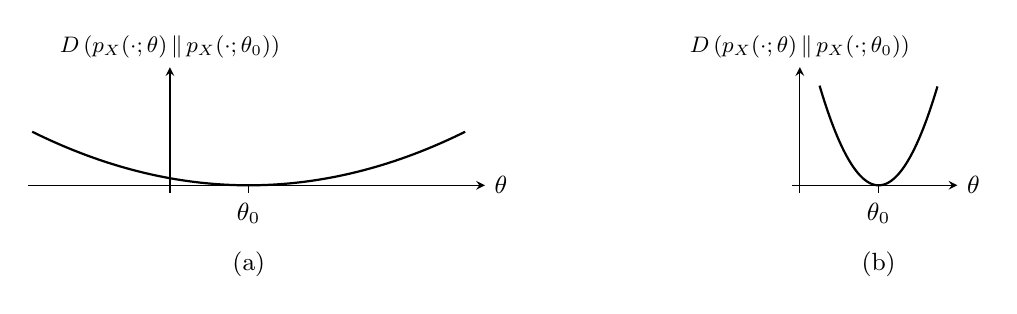
\begin{tikzpicture}
\shorthandoff{>}
%
\pgfmathsetmacro{\t}{1}
\pgfmathsetmacro{\dx}{8}
%
% peque�a curvatura
\draw[>=stealth,->] (-1.8,0)--(4,0) node[right]{\small $\theta$};
\draw[>=stealth,->] (0,-.1)--(0,1.5) node[above,scale=.9]
{\small $D\left( p_X(\cdot;\theta) \, \| \, p_X(\cdot;\theta_0) \right)$};
\draw[thick,domain=-1.75:3.75,samples=200] plot (\x,{.09*abs(\x-\t)^2});
\draw (\t,0)--(\t,-.1) node[below]{\small $\theta_0$};
%
% granda curvatura
\draw[>=stealth,->] ({-.1+\dx},0)--({2+\dx},0) node[right]{\small $\theta$};
\draw[>=stealth,->] (\dx,-.1)--(\dx,1.5) node[above,scale=.9]
{\small $D\left( p_X(\cdot;\theta) \, \| \, p_X(\cdot;\theta_0) \right)$};
\draw[thick,domain=.25:1.75,samples=200] plot ({\x+\dx},{2.25*abs(\x-\t)^2});
\draw ({\t+\dx},0)--({\t+\dx},-.1) node[below]{\small $\theta_0$};
%
\draw (\t,-1) node{\small (a)};
\draw ({\t+\dx},-1) node{\small (b)};
\end{tikzpicture}  \end{center}   \leyenda{Caso  escalar
    $\Theta \subseteq \Rset$  (para la representaci\'on) de $D$  en funci\'on de
    $\theta$.   (a) Caso  con  $J_{\theta_0}(X)$ ``peque\~no''  y  (b) caso  con
    $J_{\theta_0}(X)$ ``grande''. En el  caso (b) la determinaci\'on de $\theta$
    usando $D$ va a ser mas ``sencillo'' porque el m\'inimo es mas ``picado''.}
\label{fig:SZ:JCurvatura}
\end{figure}

\

Un otro vinculo  entre el mundo de la informaci\'on y  la estimaci\'on aparece a
trav\'es  de la  identidad de  de Bruijn~\footnote{A  pesar de  que  tom\'o este
  nombre, esta identidad  en su primera versi\'on fue publicada  por Stam. En su
  papel~\cite{Sta59}, menciona que esta identidad fue comunicada al Profesor van
  Soest por el Profesor  de Bruijn.}~\cite{Sta59, CovTho06, Joh04, Bar84, Bar86,
  PalVer06}. Esta identidad caracterisa lo  que es conocido como canal gaussiano
figura~\ref{fig:SZ:deBruijnVerdu}-(a),  \ie  la  salida  $Y$  es  una  versi\'on
ruidosa  de la  entrada. La  identidad vincula  las variaciones  de  entropia de
salida con respeto al nivel de ruido, y la informaci\'on de Fisher.

\begin{teorema}[Identidad de de Bruijn]
  Sea $X$ un  vector aleatorio continuo sobre un  abierto $\Rset^d$ y admitiendo
  una  matriz  de  covarianza,  y  sea  $Y   =  X  +  C  \Gauss$  donde  $C$  es
  deterministica, $d \times  d'$ con $ d \le d'$, de  rango m\'aximo, y $\Gauss$
  un vector gaussiano centrado y de covarianza $\Sigma_\Gauss$, independiente de
  $X$  (ver  figura~\ref{fig:SZ:deBruijnVerdu}-(a)).  Entonces, la  entropia  de
  Shannon y la informaci\'on de Fisher  de $Y$ satisfacen $$\nabla_C H(Y) = J(Y)
  \, C \, \Sigma_\Gauss$$ donde $\nabla_C  \, \cdot$ es la matriz de componentes
  $\frac{\partial \,  \cdot}{\partial C_{i,j}}$.  Si $C =  C(\theta)$ depende de
  un  parametro escalar~\footnote{Si  el parametro  es multivariado,  hace falta
    entender la  desigualdad a  trav\'es de deriva  parciales con respeto  a los
    componentes de $\theta$.}  $\theta$, $$\frac{\partial}{\partial \theta} H(Y)
  = \Tr\left( J(Y) \, C \, \Sigma_\Gauss \, \frac{\partial C^t}{\partial \theta}
  \right)$$
\end{teorema}
%
\begin{proof}
  La  clave de  este resultado  viene del  hecho de  que la  densidad $p$  de $C
  \Gauss$ satisface una ecuaci\'on diferencial particular.
  %  $$\nabla_C p_{C \Gauss}(x) =  \Hess_x p_{C
  %    \Gauss}(x) \, C \, \Sigma_\Gauss$$ Esta ecuaci\'on viene de
  La  distribuci\'on de  $C \Gauss$  se escribe  $p(x) =  (2 \pi)^{-\frac{d}{2}}
  \left| C \Sigma_\Gauss C^t  \right|^{-\frac12} \exp\left( - \frac12 x^t \left(
      C  \Sigma_\Gauss C^t  \right)^{-1} x  \right)$ (el  rango m\'aximo  de $C$
  asegura que $C \Sigma_\Gauss C^t$ sea invertible).  Para una matriz invertible
  $R$,  desarollando  $|R|$  con  respecto  a  su  linea  $i$,  se  obtiene  que
  $\frac{\partial  |R|}{\partial R_{i,j}}  = R_{i,j}^*$  cofactor  de $R_{i,j}$,
  dando por la regla de Cram\'er $\nabla_R |R| = |R| \, \left( R^{-1} \right)^t$
  (ver     tambi\'en~\cite[cap.~1~\&~9]{MagNeu99}),    es     decir    $\nabla_R
  |R|^{-\frac12}  =  -\frac12   |R|^{-\frac12}  \left(  R^{-1}  \right)^t$.   De
  $\frac{\partial |R|^{-\frac12}}{\partial  C_{i,j}} = \sum_{k,l} \frac{\partial
    |R|^{-\frac12}}{\partial R_{k,l}}  \frac{\partial R_{k,l}}{\partial C_{i,j}}
  =   -\frac12    |R|^{-\frac12}   \sum_{k,l}   \left(    R^{-1}   \right)_{l,k}
  \frac{\partial  R_{k,l}}{\partial  C_{i,j}}$ con  $R  =  C \Sigma_\Gauss  C^t$
  (simetrica)  y calculos  basicos  se obtiene  finalmente  $$\nabla_C \left|  C
    \Sigma_\Gauss  C^t  \right|^{-\frac12}  =   -  \left|  C  \Sigma_\Gauss  C^t
  \right|^{-\frac12} \left(  C \Sigma_\Gauss C^t  \right)^{-1} C \Sigma_\Gauss$$
  Ademas,  de $\left(  C \Sigma_\Gauss  C^t \right)  \left( C  \Sigma_\Gauss C^t
  \right)^{-1}   =  I$   viene  $\frac{\partial   \left(  C   \Sigma_\Gauss  C^t
    \right)^{-1}}{\partial C_{i,j}} = -  \left( C \Sigma_\Gauss C^t \right)^{-1}
  \frac{\partial \left( C \Sigma_\Gauss  C^t \right)}{\partial C_{i,j}} \left( C
    \Sigma_\Gauss  C^t  \right)^{-1}$ donde  $e_i$  es el  vector  con  1 en  su
  componente $i$ y cero si no, dando
  %
  \begin{eqnarray*}
  \frac{\partial \left( x^t \left( C \Sigma_\Gauss C^t \right)^{-1} x
  \right)}{\partial C_{i,j}} & = & - x^t \left( C \Sigma_\Gauss C^t \right)^{-1}
  \left( e_i e_j^t \Sigma_\Gauss C^t + C \Sigma_\Gauss e_j e_i^t \right) \left( C
  \Sigma_\Gauss C^t \right)^{-1} x\\[2.5mm]
  %
  & = & - 2 \, e_i^t \left( C \Sigma_\Gauss C^t \right)^{-1} x x^t \left( C
  \Sigma_\Gauss C^t \right)^{-1} C \Sigma_\Gauss e_j
  \end{eqnarray*}
  %
  usando $x^t A e_k e_l^t  B x = e_l^t B x x^t A e_k =  e_k^t A^t x x^t B^t e_l$
  (escalares  comutan y  un  escalar es  igual  a su  transpuesta)  y usando  la
  simetria de  $C \Sigma_\Gauss C^t$.   Eso significa que $$\nabla_C  \left( x^t
    \left(  C  \Sigma_\Gauss C^t  \right)^{-1}  x  \right) =  -  2  \, \left(  C
    \Sigma_\Gauss C^t \right)^{-1} x x^t \left( C \Sigma_\Gauss C^t \right)^{-1}
  C \Sigma_\Gauss,$$ dando $$\nabla_C p(x) = \left( - \left( C \Sigma_\Gauss C^t
    \right)^{-1}  + \left(  C  \Sigma_\Gauss  C^t \right)^{-1}  x  x^t \left(  C
      \Sigma_\Gauss C^t  \right)^{-1} \right) C \Sigma_\Gauss  \, p(x)$$ Tomando
  la  Hessiana  de $p$  con  respeto  a $x$  se  obtiene  sencillamente que  $p$
  satisface  la  ecuaci\'on  diferencial  $$\nabla_C  p  = \Hess_x  p  \,  C  \,
  \Sigma_\Gauss$$  Suponiende que  se puede  intervertir derivadas  y integrales
  (ver~\cite{Bar84, Bar86}  donde se dan  condiciones rigorosas), $\displaystyle
  p_Y(y) = \int_{\Rset^d} p_X(x) p(y-x) \, dx$ satisface tambi\'en la ecuaci\'on
  diferencial, y ademas
  %
  \begin{eqnarray*}
  \nabla_C H(Y) & = & - \int_{\Rset^d} \nabla_C \, p_Y(y) \log p_Y(y)
  \, dy - \int_{\Rset^d} \nabla_C \, p_Y(y) \, dy\\[2.5mm]
  %
  & = & - \left( \int_{\Rset^d} \Hess_y \, p_Y(y) \log p_Y(y) \, dy \right) C \,
  \Sigma_\Gauss - \nabla_C \int_{\Rset^d} p_Y(y) \, dy\\[2.5mm]
  %
  & = & - \left( \int_{\Rset^d} \left( \Hess_y \Big( p_Y(y) \log p_Y(y) \Big) -
  \Hess_y \, p_Y(y) - \frac{\nabla_y \, p_Y(y) \, \nabla_y \, p_Y(y)^t}{p_Y(y)}
  \right) \, dy \right) C \, \Sigma_\Gauss\\[2.5mm]
  %
  & = & - \left( \int_{\Rset^d} \Hess_y \Big( p_Y(y) \log p_Y(y) \Big) \, dy -
  \int_{\Rset^d} \Hess_y p_Y(y) \, dy \right) C \, \Sigma_\Gauss \: + \: J(Y) \, C
  \, \Sigma_\Gauss
  \end{eqnarray*}
  %
  usando la  ecuaci\'on diferencial en la  secunda linea, el hecho  de que $p_Y$
  suma  a  1  en  la  tercera  linea  (su gradiente  es  cero  entonces),  y  la
  definici\'on de la matriz de Fisher en la \'ultima linea. Usando el teorema de
  la  divergencia (intergraci\'on  por  partes) aplicada  respectivamente a  los
  componentes de $\nabla_y p_Y \log  p_Y$ y $\nabla_y p_Y$, suponiendo que estos
  gradientes  se cancelan  en el  borde del  dominio de  integraci\'on,  los dos
  terminos  integrales valen cero,  lo que  cierra la  prueba de  la desigualdad
  general.   Ademas,  si  $C  =  C(\theta)$, la  secunda  desigualdad  sigue  de
  $\frac{\partial   \cdot}{\partial    \theta}   =   \sum_{i,j}   \frac{\partial
    \cdot}{\partial   C_{i,j}}   \frac{\partial   C_{i,j}}{\partial  \theta}   =
  \Tr\left( \nabla_C \, \frac{\partial C^t}{\partial \theta} \right)$.
\end{proof}

La  versi\'on  inicial  de la  identidad  de  de  Bruijn, con  $\Sigma_\Gauss  =
I$,   $$\frac{d}{d\theta}   H(X+\sqrt{\theta}   \Gauss)  =   \frac12   \Tr\left(
  J(X+\sqrt{\theta} \Gauss)  \right)$$ se  recupera en el  caso particular  $C =
\sqrt{\theta}  I$.  En  este caso,  la ecuac\'ion  diferencial satisfada  por la
densidad de probabilidad $p$ es la {\it ecuaci\'on del calor}.  Esta desigualdad
cuantifica las variaciones de entropias bajo varaciones de ``niveles'' del ruido
del canal de comunicaci\'on. De una forma, caracteriza la robustez del canal con
respeto al nivel de ruido gaussiano  (la gaussiana juega de nuevo un rol central
ac\'a).

\

Existe una  otra forma  muy similar  de esta desigualdad  debido a  Guo, Shamai,
Verd\'u, Palomar~\cite{GuoSha05, PalVer06}. Esta versi\'on vincula a\'un mas los
mundo  de  la   informaci\'on  y  el  de  la  estimaci\'on.    Del  lado  de  la
comunicaci\'on, consiste a caracterisar  la informaci\'on mutua entre la entrada
$X$ de un canal  ruidoso y su salida, $Y = B X +  \Gauss$ donde $B$ coresponde a
un  pre-tratamiento antes  de la  salida, figura~\ref{fig:SZ:deBruijnVerdu}-(b).
Del lado de  la estimaci\'on, uno puede querer  estimar $X$ observando solamente
$Y$.  Es  conocido que el estimador  que minimiza el  error cuandratico promedio
$\Esp\left[  \left\| \widehat{X}(Y)  -  X \right\|^2  \right]$  es la  esperanza
condicional  $\widehat{X}(Y) =  \Esp[X|Y]$. Una  caracteristica de  un estimador
siendo su  matriz de covarianza,  se notar\'a $\E(X|Y)  = \Esp\left[ \left(  X -
    \Esp[X|Y]  \right) \left(  X  - \Esp[X|Y]  \right)^2  \right]$ esta  matriz.
Sorpredentemente,  existe  tambi\'en  una  identidad  entre \  $I(X;Y)$  \  y  \
$\E(X|Y)$:
%
\begin{teorema}[Identidad de Guo--Shamai--Verd\'u]
  Sea  $X$  un  vector  aleatorio  continuo  sobre  un  abierto  $\Rset^{d'}$  y
  admitiendo una  matriz de covarianza, y  sea $Y = B  X + \Gauss$  donde $B$ es
  deterministica, $d  \times d'$, y $\Gauss$  un vector gaussiano  centrado y de
  covarianza      $\Sigma_\Gauss$,      independiente      de      $X$      (ver
  figura~\ref{fig:SZ:deBruijnVerdu}-(b)). Entonces, la informaci\'on mutua entre
  \ $X$ \  e \ $Y$ y la  matriz de covarianza del estimador  de error cuadratico
  m\'inimo satisfacen  $$\nabla_B I(X;Y) = \Sigma_\Gauss^{-1} B  \, \E(X|Y)$$ Si
  $B      =     B(\theta)$     depende      de     un      parametro     escalar
  $\theta$,    $$\frac{\partial}{\partial    \theta}    I(X;Y)    =    \Tr\left(
    \Sigma_\Gauss^{-1} \,  B \, \E(X|Y) \,  \frac{\partial B^t}{\partial \theta}
  \right)$$
\end{teorema}
%
\begin{proof}
  Notando  que  $p_{Y|X} (y,x)  =  (2  \pi)^{-\frac{d}{2}} \left|  \Sigma_\Gauss
  \right|^{-\frac12}  \exp\left( -\frac12  (y-B  x)^t \Sigma_\Gauss^{-1}  (y-Bx)
  \right)$ viene $\nabla_B p_{Y|X}(x,y)  = p_{Y|X}(x,y) \, \Sigma_\Gauss^{-1} (y
  - B x) x^t$  (ver unos pasos de la prueba de la  identidad de de Bruijn) as\'i
  que $\nabla_y  p_{Y|X}(y,x) = p_{Y|X}(y,x)  \, \Sigma_\Gauss^{-1} (y -  B x)$,
  dando  $$\nabla_B p_{Y|X}(y,x)  =  \nabla_y p_{Y|X}(y,x)  x^t \qquad  \mbox{y}
  \qquad  \nabla_B  p_{X,Y}(x,y) =  \nabla_y  p_{X,Y}(x,y) x^t$$  (multiplicando
  ambos lados por $p_X$. Ahora, $I(X;Y) =  H(Y) - H(Y|X) = H(Y) - H(\Gauss)$ (de
  la  independencia, cuando  $X =  x$, $Y  = B  x +  \Gauss$ gaussiana  de misma
  convarianza que $\Gauss$ y de promedio $B x$), as\'i que
  %
  \begin{eqnarray*}
  \nabla_B I(X;Y) & = & \nabla_B H(Y)\\[2.5mm]
  %
  & = & - \int_{\Rset^d \times \Rset^{d'}} \nabla_B \Big( p_{X,Y}(x,y) \, \log
  p_Y(y) \Big) \, dx \, dy\\[2.5mm]
  %
  & = & - \int_{\Rset^d \times \Rset^{d'}} \nabla_B \, p_{X,Y}(x,y) \, \log p_Y(y) \,
  dx \, dy - \int_{\Rset \times \Rset} p_{X|Y}(x,y) \, \nabla_B \, p_Y(y) \, dx \,
  dy\\[2.5mm]
  %
  & = & \int_{\Rset^d \times \Rset^{d'}} \nabla_y p_{X,Y}(x,y) \, x^t \log p_Y(y)
  \, dx \, dy - \int_{\Rset^d} \nabla_B p_Y(y) \, dy\\[2.5mm]
  %
  & = & - \int_{\Rset^d \times \Rset^{d'}} \nabla_y p_Y(y) x^t p_{X|Y}(x,y) \, dx
  \, dy\\[2.5mm]
  %
  & = & - \int_{\Rset^d} \nabla_y p_Y(y) \, \Esp\left[X^t | Y = y \right] \, dy
  \end{eqnarray*}
  %
  La secunda linea  viene de la escritura de $H(Y)$  usando $p_Y$ como marginale
  de $p_{X,Y}$  en $x$ y  intercambiando gradiente e  integral (ver pasos  de la
  prueba de la desigualdad de de Bruijn); la tercera de $p_{X,Y}/p_Y = p_{X|Y}$;
  en la cuarta  se usa la ecuaci\'on diferencial satisfecha  por $p_{X,Y}$ en la
  primera integral y  integrando en $x$ en la secunda  integral; la quinta linea
  se obtiene usando el teorema  de la divergencia (intergraci\'on por partes) en
  la integraci\'on en  $y$ de la primera integral,  e intercambiando gradiente e
  integral el la secunda ($p_Y$ sumando a 1, el termino se cancela). Ademas,
  %
  \begin{eqnarray*}
  \nabla_y p_Y(y) & = & \int_{\Rset^{d'}} \nabla_Y p_{Y|X}(y,x) \, p_X(x) \,
  dx\\[2.5mm]
  %
  & = & - \Sigma_\Gauss^{-1} \int_{\Rset^{d'}} (y - B x) \, p_{Y|X}(y,x) \, p_X(x) \,
  dx\\[2.5mm]
  %
  & = & - \Sigma_\Gauss^{-1} \left( y - B \int_{\Rset^{d'}} x \, p_{X|Y}(x,y) \,dx
  \right) p_Y(y)\\[2.5mm]
  %
  & = & - \Sigma_\Gauss^{-1} \Big( y - B \Esp\left[X | Y=y \right] \Big) \, p_Y(y)
  \end{eqnarray*}
  %
  escribiendo $p_{Y|X}(y,x)  \, p_X(x) =  p_{X|Y}(x,y) \, p_Y(y)$ en  la tercera
  linea. Esta ecuaci\'on permite escribir
  %
  \begin{eqnarray*}
  \nabla_B I(X;Y) & = & \Sigma_\Gauss^{-1} \int_{\Rset^d} \Big( y - B \Esp\left[X |
  Y=y \right] \Big) \Esp\left[X^t | Y=y \right] \, p_Y(y) \, dy\\[2.5mm]
  %
  & = & \Sigma_\Gauss^{-1} \left( \Esp\left[ Y \Esp\left[ X^t|Y \right] \right] - B
  \Esp\left[ \Esp\left[X | Y \right] \Esp\left[X | Y \right]^t \right]
  \right)\\[2.5mm]
  %
  & = & \Sigma_\Gauss^{-1} \left( \Esp\left[ Y X^t \right] - B \Esp\left[ \Esp\left[X
  | Y \right] \Esp\left[X | Y \right]^t \right] \right)\\[2.5mm]
  %
  & = & \Sigma_\Gauss^{-1} B \left( \Esp\left[ X X^t \right] - \Esp\left[
  \Esp\left[X | Y \right] \Esp\left[X | Y \right]^t \right] \right)
  \end{eqnarray*}
  %
  la \'ultima linea viniendo de $Y = B X + \Gauss$ con $\Gauss$ independiente de
  $X$ y  de promedio 0.  La  prueba se cierra notando  que $\Esp\left[ \Esp[X|Y]
  \right] = \Esp[X]$ y por  la formula de K\"onig-Huyggens. La secunda identidad
  viene  de  $\frac{\partial \cdot}{\partial  \theta}  =  \Tr\left( \nabla_B  \,
    \frac{\partial B^t}{\partial \theta} \right)$ (ver prueba de la identidad de
  de Bruijn).
\end{proof}
%
\noindent La primera versi\'on de esta identidad se recupera con $B = \sqrt{s}$,
$\Sigma_\Gauss  =  I$  y $X$  de  covarianza  identidad;  $s$ es  conocido  como
relaci\'on se\~nale/ruido es este caso.

Existen versiones  a\'un mas completas (con  gradientes con respeto  a la matriz
$\Sigma_\Gauss$ por  ejemplo) que se pueden  consultar en~\cite{Joh04, PalVer06,
  PayPal09}.

\begin{figure}[h!]
  \begin{center}  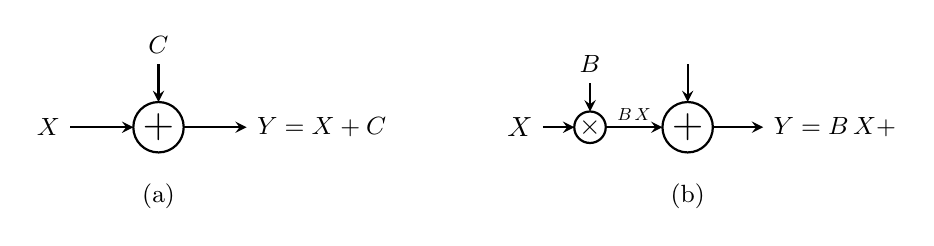
\begin{tikzpicture}[scale=.8]
\shorthandoff{>}
%
\begin{scope}
\draw[>=stealth,->,thick] (0,0) node[left]{\small $X$} --(1,0);
\draw[thick] (1.4,0) circle (.4);
\draw[>=stealth,->,thick] (1.4,1) node[above]{\small $C \Gauss$} --(1.4,.4);
\draw (1.4,0) node[align=center,scale=1.25]{\large +};
\draw[>=stealth,->,thick] (1.8,0)--(2.8,0) node[right]{\small $Y = X + C \Gauss$};
%
\end{scope}
%
\begin{scope}[xshift=7.5cm]
\draw[>=stealth,->,thick] (0,0) node[left]{$X$} --(.5,0);
\draw[thick] (.75,0) circle (.25);
\draw[thick] (.75,0) node[align=center]{$\times$};
\draw[>=stealth,->,thick] (.75,.7) node[above]{\small $B$} --(.75,.25);
\draw[>=stealth,->,thick] (1,0)--(1.9,0);
\draw[thick] (1.45,0) node[align=center,scale=.7,above]{\small $B \, X$};
\draw[thick] (2.3,0) circle (.4);
\draw[>=stealth,->,thick] (2.3,1) node[above]{\small $\Gauss$} --(2.3,.4);
\draw (2.3,0) node[align=center,scale=1.25]{\large +};
\draw[>=stealth,->,thick] (2.7,0)--(3.5,0) node[right]{\small $Y = B \, X + \Gauss$};
%
\end{scope}
\draw (1.4,-1.1) node {\small (a)};
\draw (9.8,-1.1) node {\small (b)};
\end{tikzpicture}
 \end{center}  \leyenda{Canal de
    comunicaci\'on gaussiano  de entrada $X$.  (a) Canal  gaussiano usual, donde
    $C$ maneja los parametros (nivel) del  ruido. (b) canal con gaussiano con un
    preprocesamiento $B$ de la entrada.}
\label{fig:SZ:deBruijnVerdu}
\end{figure}
\

De la desigualdad de la potencia entropica  y de la identidad de de Bruijn surge
una otra desigualdad implicando la  potencia entropica $N$ y la informaci\'on de
Fisher $J$. Esta desigualdad es conocida como desigualdad de Stam~\footnote{Como
  por  la identidad  de  de Bruijn,  stam  mencion\'o que  esta desigualdad  fue
  comunicada al Profesor van Soest por el Profesor de Bruijn quien da una prueba
  variacional  de  la desigualdad.}~\cite{CovTho06,  Rio07,  Sta59},  o a  veces
``desigualdad isoperimetrica para la entropia''~\cite{WanMad04}.
%
\begin{teorema}[Desigualdad de Stam]
  Sea   $X$    una   variable    aleatoria   continua   sobre    $\D   \subseteq
  \Rset^d$. Entonces, $$N(X)  \Tr\left( J(X) \right) \, \ge  \, d$$ con igualdad
  si y solamente si $X$ es gaussiano de covarianza proporcional a la identidad.
\end{teorema}
%
\begin{proof}
  De la  desigualdad de  la potencia entropica  se obtiene $N(X  + \sqrt{\theta}
  \Gauss)  \ge N(X)  + \theta  \left| \Sigma_\Gauss  \right|^{\frac1d}$. Tomando
  $\Sigma_\Gauss  = I$,  se obtiene  $\forall  \, \theta  > 0,$  \ $\frac{N(X  +
    \sqrt{\theta} \Gauss)  - N(X)}{\theta} \ge  $.  Entonces, tomando  el limite
  $\theta  \to 0$,  aparece que  $\left. \frac{d}{d\theta}  N(X  + \sqrt{\theta}
    \Gauss)   \right|_{\theta  =   0}  \ge   1$.   La   prueba  se   cierra  con
  $\frac{d}{d\theta}  N(X   +  \sqrt{\theta}   \Gauss)  =  \frac{1}{2   \pi  \e}
  \frac{d}{d\theta}  \exp\left( \frac2d  H(X +  \sqrt{\theta} \Gauss)  \right) =
  \frac2d  N(X +  \sqrt{\theta}  \Gauss) \frac{d}{d\theta}  H(X +  \sqrt{\theta}
  \Gauss) = d N(X +  \sqrt{\theta} \Gauss) \Tr\left( J(X + \sqrt{\theta} \Gauss)
  \right)$  (por la identitad  de de  Bruijn).  Ademas,  la igualdad  se obtiene
  cuando se obtiene  la igualdad en la desigualdad de  la potencia entropica, es
  decir cuando $X$ es gaussiano de  varianza proporcional a la del ruido, que es
  la identidad en este caso.
\end{proof}
%
Se  puede  ver  de  nuevo  el  rol  central  que  juega  la  gaussiana  en  esta
desigualdad. Ademas,  de la desigualdad de  Stam se puede  deducir tamb\'ien las
versiones escalares de la desigualdad Cram\'er-Rao. Viene del hecho de que, dado
una matriz de covarianza, le entropia  $H(X)$ es maxima cuando $X$ es gaussiano.
Entonces, para cualquier $X$ de covarianza $\Sigma_X$, $N(X) \le \left| \Sigma_X
\right|^{\frac1d}$,   dando  de   la  desiguldad   de  Stam,   $\left|  \Sigma_X
\right|^{\frac1d} \Tr\left( J(X) \right) \ge d$ (y las otras versiones escalares
de la relaci\'on  determinente-traza).  Como se lo puede  esperar, se obtiene la
igualdad si y solamente $X$  es gaussiana (potencia entropica alcanzando su cota
superior) y de matriz la identidad (desiguladad de Stam se saturando).

Varias otras pruebas de la desigualdad de Stam pueden venir de generalizaciones,
por ejemplo debido a Lutwak o Bercher~\cite{Lut, Ber}. {\color{red} La secci\'on
  ZZZ lo va a rapidamente evocar.}

\

{\color{red}\bf   Existe un data proc ineq con Fisher, cf Rioul 07 ou Stam 59}



% ================================== Mutua =================================== %

\seccion{Unos ejemplos y aplicaciones}
\label{s:SZ:Ejemplos}


% ================================= canal

\subseccion{Canal de transmisi\'on y su capacidad}
\label{ss:SZ:CanalCapacidad}

Siguiendo el  esquema de comunicaci\'on de  Shannon, un mensaje  que se modelisa
como  un vector  aleatorio~\footnote{De  punto  de vista  de  un receptor,  este
  mensaje es  desconocido. Ademas,  se lo  puede ver como  una instancia  de una
  clase  importante   de  posibles  mensajes,   justificando  la  modelisaci\'on
  aleatoria.} $X$  pasa por un  canal de comunicaci\'on  y se recibe  un mensaje
$Y$, vector  aleatorio. En el trabajo de  Shannon, el canal es  supuesto a ruido
additiva,  es decir que  se a\~nade  un ruido  a $X$.   De manera  general, para
conocer la informaci\'on de $X$ que se recibe, se calcula la informaci\'on mutua
$I(X;Y)$, es decir  la cuantidad de informaci\'on que comparten  la entrada y la
salida del canal.   Lo mas $I$ es grande, lo mas  de informaci\'on se transmite.
Dado el canal,  se puede arreglar $X$ (su distribuci\'on)  de manera a maximizar
$I(X;Y)$, es decir la cantidad maxima  que se puede transmitir en este canal. Es
lo que  es conocido como capacidad  del canal~\cite[part.~II~\&~III]{Sha48} (ver
tambi\'en~\cite{CovTho06, Rio07} entre otros):
%
\begin{definicion}[Capacidad de canal]
  Sea un canal de transmici\'on, $X$  su entrada e $Y$ su salida, como ilustrado
  figura~\ref{fig:SZ:CanalComunicacion}.   Sea   $p_X$   la  distribuci\'on   de
  probabilidad  de  $X$. La  capacidad  $C$  del canal  es  definida  por $$C  =
  \max_{p_X} \, I(X;Y)$$
\end{definicion}

\begin{figure}[h!]
  \begin{center}  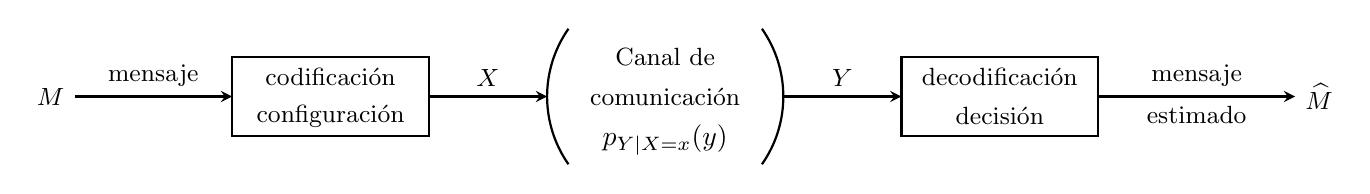
\begin{tikzpicture}
\shorthandoff{>}
%
% Mensaje
\draw[>=stealth,->,thick] (0,0) node[left]{\small $M$} --(2,0);
\node[above] at (1,0){\small mensaje};
%
% codificacion
\draw[thick] (2,-.5) rectangle (4.5,.5);
\node at (3.25,.25){\small codificaci\'on};
\node at (3.25,-.25){\small configuraci\'on};
%
% entrada del canal
\draw[>=stealth,->,thick] (4.5,0)--(6,0);
\node[above] at (5.25,0){\small $X$};
%
% Canal de com
\pgfmathsetmacro{\t}{35};
\pgfmathsetmacro{\r}{1.5};
\draw[thick] ({6+\r*(1+cos(180-\t))},{\r*sin(\t)}) arc (180-\t:180+\t:\r);
\draw[thick] ({6+\r*(1+cos(\t))},{-\r*sin(\t)}) arc (-\t:\t:\r);
\node at ({6+\r},.5){\small Canal de};
\node at ({6+\r},0){\small comunicaci\'on};
\node at ({6+\r},-.55){$p_{Y|X=x}(y)$};
%
% salida
\draw[>=stealth,->,thick] ({6+2*\r},0)--({7.5+2*\r},0);
\node[above] at ({6.75+2*\r},0){\small $Y$};
%
% decodificacion/decision
\draw[thick] ({7.5+2*\r},-.5) rectangle ({10+2*\r},.5);
\node at ({8.75+2*\r},.25){\small decodificaci\'on};
\node at ({8.75+2*\r},-.25){\small decisi\'on};
%
% Mensaje estimado
\draw[>=stealth,->,thick] ({10+2*\r},0)--({12.5+2*\r},0) node[right]{\small $\widehat{M}$};
\node[above] at ({11.25+2*\r},0){\small mensaje};
\node[below] at ({11.25+2*\r},0){\small estimado};
\end{tikzpicture}
  \end{center} \leyenda{Esquema
    de  comunicaci\'on de  Shannon.   En una  primera  etapa, un  mensaje $M$  a
    transmitir  es  c\'odificado  (ej.  c\'odigo  binario)  o  puesto  en  forma
    (ej.  simbolos modulando una  funci\'on para  que sea  anal\'ogica y  en una
    banda  frecuencial  dada). Sea  $X$  este  mensaje  codificado o  puesto  en
    forma. A la recepci\'on, se mide  $Y$ (ej. versio\'on ruidosa de $X$), antes
    de ser decodificado o usado  para tomar una decisi\'on, $\widehat{M}$ siendo
    la estimaci\'on de  $M$ (ej. simbolos estimados a partir  de $Y$). Una etapa
    importante es el vinculo entre la entrada  $X$ y la salida $Y$ del canal, es
    decir la cantidad de informaci\'on  que tienen en com\'un.  La capacidad del
    canal es la informaci\'on $I(X;Y)$ m\'axima con respeto a su entrada.}
%~\cite{Sha48}.}
\label{fig:SZ:CanalComunicacion}
\end{figure}


% ================================= canal binario

\subsubseccion{Canal binario}

Suponiendo  que el  mensaje  mandado en  un  canal es  una  cadena de  simbolos,
variables   aleatorias  independientes,   se  puede   concentrarse   sobre  cada
simbolo. En  este marco, un  canal de comunicaci\'on  lo mas simple  es conocido
como  {\it canal  binario}~\cite[Sec.~15]{Sha48}: $X$  es una  variable definida
sobre  $\A =  \{ 0  , 1  \}$;  tal tipo  de entrada  es natural,  pensando a  la
c\'odificaci\'on binaria.   La salida $Y$  es tambi\'en definida sobre  $\A$; se
puede imaginar medir y tomar una decisi\'on binaria usando la medida.  Tal canal
es   definido  por  sus   probabilidad  de   transici\'on  $p_{Y|X}$,   \ie  las
probabilidades que un 0 (resp. un 1)  se transmite corectamente o cambia en un 1
(resp. 0),  \ie \ $$p  = \Pr[Y = 1  | X =  0] = 1  - \Pr[Y =  0 | X =  0] \qquad
\mbox{y} \qquad q  = \Pr[Y = 0  | X = 1] =  1 - \Pr[Y =  1 | X = 1]$$  $p$ y $q$
representan    errores    de   comunicaci\'on.     Tal    canal   es    descrito
figura~\ref{fig:SZ:CanalBinario}-(a).   La  figura~\ref{fig:SZ:CanalBinario}-(b)
da un esquema ``f\'isico'' que puede se  al origen de tal canal. Cuando $p = q$,
el canal es conocido como {\it canal binario simetrico}. Cuando $p = 0$ y $q \in
(0 \, ; \, 1)$, el canal es conocido como {\it canal binario en Z}.

\begin{figure}[h!]
\begin{center}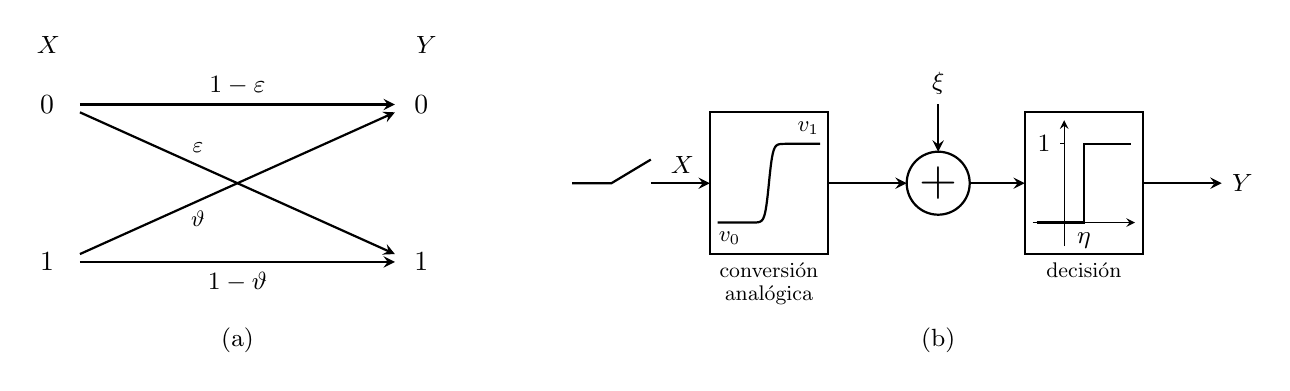
\begin{tikzpicture}
\shorthandoff{>}
%
\begin{scope}
\node at  (-.4,1.75){\small $X$}; \node at  (4.4,1.75){\small $Y$};
%
\draw[>=stealth,->,thick] (-.2,1) node[left]{0} (0,1) -- (4,1) node[right]{\ 0};
\node[above] at (2,1){\small $1-\varepsilon$};
%
\draw[>=stealth,->,thick] (-.2,-1) node[left]{1} (0,-1) -- (4,-1) node[right]{\ 1};
\node[below] at (2,-1){\small $1-\vartheta$};
%
\draw[>=stealth,->,thick] (0,.9)--(4,-.9);
\node[scale=.9] at (1.5,.45){\small $\varepsilon$};
%
\draw[>=stealth,->,thick] (0,-.9)--(4,.9);
\node[scale=.9] at (1.5,-.45){\small $\vartheta$};
%
\end{scope}
%
\begin{scope}[xshift=7cm]
%
% entrada
\draw[thick] (-.75,0)--(-.25,0)--(.25,.3);
\draw[>=stealth,->,thick] (.25,0)--(1,0);
%\draw[>=stealth,->,thick] (.25,-.5) node[below]{\small $X$} --(.25,.1);
\node[above] at (.65,0){\small $X$};
%
% puesta en niveles
\draw[thick] (1,-.9) rectangle (2.5,.9);
\node[scale=.9] at (1.25,-.7){\small $v_0$};
\node[scale=.9] at (2.25,.7){\small $v_1$};
\draw[thick,domain=-4.5:4.5,samples=100] (1.1,-.5) -- plot ({\x/10+1.75},{.5*tanh(2*\x)}) --(2.4,.5);
\node[below,scale=.85] at (1.75,-.9){\small conversi\'on};
\node[below,scale=.85] at (1.75,-1.2){\small anal\'ogica};
%
% adicion del ruido
\draw[>=stealth,->,thick] (2.5,0)--(3.5,0);
\draw[thick] (3.9,0) circle (.4);
\draw[>=stealth,->,thick] (3.9,1) node[above]{\small $\xi$} --(3.9,.4);
\node[align=center,scale=1.5] at (3.9,0){\large +};
%
% decision
\draw[>=stealth,->,thick] (4.3,0)--(5,0);
\draw[thick] (5,-.9) rectangle (6.5,.9);
\draw[>=stealth,->] (5.1,-.5)--(6.4,-.5);
\draw[>=stealth,->] (5.5,-.8)--(5.5,.8);
\draw[thick] (5.15,-.5)--(5.75,-.5)--(5.75,.5)--(6.35,.5);
\node[below] at (5.75,-.5){\small $\eta$};
\draw (5.5,.5)--(5.45,.5) node[left]{\small 1};
\node[below,scale=.85] at (5.75,-.9){\small decisi\'on};
%
% salida
\draw[>=stealth,->,thick] (6.5,0)--(7.5,0) node[right]{\small $Y$};
\end{scope}
\node at (2,-2){\small (a)};
\node at (10.9,-2){\small (b)};
\end{tikzpicture}
\end{center}
\leyenda{(a): canal  binario. La entrada  $X$ definida sobre  $\A = \{ 0  , 1\}$
  pasa  por este canal  e $Y$  definida sobre  $\A$ es  recibido. Este  canal es
  caracterisado por  las probabilidades  de transition $p_{Y|X}$.   (b): Esquema
  que puede conducir  al canal binario; una variable puede ser  la salida de una
  puerta  l\'ogica, con  niveles $v_0$  (nivel  bajo, c\'odificando  0) y  $v_1$
  (nivel  alto,  c\'odificando  1).   Se  puede imaginar  que  este  voltaje  es
  transmitido por  un canal  a\~nandido un ruido  $\xi$.  En la  recepci\'on, se
  toma una  decisi\'on, por ejemplo  0 (resp.  1)  si la medida es  mayor (resp.
  menor) que $\eta = \frac{v_0 + v_1}{2}+\Esp[\xi]$.  En este ejemplo, $p$ y $q$
  van a  ser caracterisada completamente por  la distribuci\'on del  ruido (y de
  los deos niveles posibles de la entrada), pero no de la distribuci\'on $p_X$.}
%~\cite{Sha48}.}
\label{fig:SZ:CanalBinario}
\end{figure}

{\color{red}\bf mettre le canal a effacement?}

En este caso, trabajando con bits, el logaritmo lo mas l\'ogico es el de base 2,
dando una capacidad en bits. Sea $$\alpha = \Pr[X = 0]$$ dando la distribuci\'on
de la entrada. La distribuci\'on de la salida va a ser dada a partir de $\beta =
\Pr[Y = 0] = \Pr[Y =  0 | X = 0] \Pr[X = 0] + \Pr[Y = 0 |  X = 1] \Pr[X = 1]$ es
decir $$\beta  = \Pr[Y =  0] =  q + \alpha  (1-p-q)$$ La informaci\'on  mutua se
escribe $I(X;Y) = H(Y) - H(Y|X) = H(Y)  - H(Y|X=0) \Pr[X = 0] + H(Y|X=1) \Pr[X =
1]$, lo que  toma la expresi\'on $$I(X;Y) = h(\beta) -  \alpha h(p) - (1-\alpha)
h(q)$$  donde  $h(\lambda) =  -  \lambda  \log_2  \lambda -  (1-\lambda)  \log_2
(1-\lambda)$ es  la entropia  binaria en bits.  Para calcular la  capacidad $C$,
hace  falta  m\'aximizar $I$  con  respeto  a  $\alpha$.  Diferenciando  $I$  en
$\alpha$,   \ie  $\frac{\partial   I(X;Y)}{\partial  \alpha}   =  \frac{\partial
  h(\beta)}{\partial  \beta}  \frac{\partial \beta}{\partial  \alpha}  - h(p)  +
h(q)$,  es  decir $$\frac{\partial  I(X;Y)}{\partial  \alpha}  = (1-p-q)  \log_2
\left( \frac{1-\beta}{\beta} \right) - h(p) + h(q)$$
%
\begin{itemize}
\item Claramente, $$q =  1-p \quad \Rightarrow \quad C = 0$$  Viene del hecho de
  que  para  $q  =  1-p$,  de  $h(p)  = h(1-p)$  se  deduce  que  $I(X;Y)  =0  $
  constante. De hecho, en  este caso, un 0 en la salida puede venir  de un 0 o 1
  con probabilida igual, y  lo mismo para un 1 en la  salida; en otros terminos,
  la salida  aparece independiente de  la entrada.  Eso se  verifica formalmente
  con $\beta = q$, dando $p_{Y|X}  = p_Y$, dando una informaci\'on mutua cero, y
  entonces una capacidad cero.
%
\item Si $q  \ne 1-p$, la derivada de  $I$ con respeto a $\alpha$  se anula para
  $\beta    =   \beta^\opt$   ($\alpha    =   \alpha^\opt$),    $$\beta^\opt   =
  \frac{1}{1+2^{\frac{h(p)-h(q)}{1-p-q}}}     \qquad     \mbox{siendo}    \qquad
  \alpha^\opt = \frac{\beta^\opt  - q}{1-p-q}$$ y dando un  extremo para $I$.  A
  continuaci\'on,      $\frac{\partial^2       I}{\partial      \alpha^2}      =
  \frac{(1-p-q)^2}{\beta  (1-\beta)}  >  0$   (en  particular  para  le  $\beta$
  ``\'optimo''),  probando  de que  el  extremo  es  un m\'aximo.   Poniendo  el
  $\alpha^\opt$ en la  formula de $I(X;Y)$, luego de  muchos calculos (basicos),
  se  obtiene  $$C =  \log_2\left(  1  +  2^{\frac{h(p)-h(q)}{1-p-q}} \right)  -
  \frac{1-q}{1-p-q} h(p)  + \frac{p}{1-p-q} h(q)$$  Cuando $q \to  1-p$, notando
  que $h(p) =  h(1-p)$ y tomando el  limite de esta formula, se  recupera que $C
  \to 0$.
  %
  % ---
  %
%  \newline{\color{red}\bf   �Interpretacion?    no   hay   combinacion   convexa
%    $\frac{p}{1-p-q}$ siendo del mismo signo que $\frac{1-q}{1-p-q}$; nota: $C =
%    \log_2\left(  1  + 2^{-  \frac{h(1-q)-h(p)}{(1-q)-p}}  \right) +  \frac{1}{p
%      (1-q)} \frac{(1-q) h(1-q) - p h(p)}{q - (1-p)}$}
\end{itemize}
%
\noindent De \ $I(X;Y) =  H(Y) - H(Y|X) \le H(Y) \le 1$ bit  \ ($Y$ es binario, de
entropia maxima en  el caso uniforme), aparece sin calculos que  $$C \le 1$$ \ie
la capacidad es menor que 1  bit~\footnote{De manera general, de la escritura de
  $I$  con entropias condicionales,  para $X$  definido sobre  $\A$ e  $Y$ sobre
  $\B$, da $0 \le C \le \min( \log  |\A| \, , \, \log |\B| )$. Ademas, $p_{Y|X}$
  depende solo  del canal  y no  de la entrada,  as\'i que  para $p_X  = \lambda
  p_X^{(1)}  + (1-\lambda)  p_X^{(2)}$ se  obtiene  $p_Y =  \lambda p_Y^{(1)}  +
  (1-\lambda) p_Y^{(2)}$ con $p_Y^{(i)}$  salida corespondiente a $p_X^{(i)}$ de
  $I(X;Y) = H(Y)-H(Y|X)$,  el secundo termino dependiente solo  del canal, de la
  concavidad de  $H$ se obtiene  que $I$ es  concava con respeto a  $p_X$. $p_X$
  parteciendo a  un convexo, $I$  tiene un m\'aximo, \'unico.}:  para transmitir
informaci\'on en  este canal, hace  falta introducir redundancia en  el mensaje.
Se alcanza  $C = 1$ si, (i)  por un lado $H(Y|X)  = 0$, es decir  $\alpha h(p) +
(1-\alpha) h(q)  = 0$ y (ii) ademas  $h(\beta) = 1$.  Estudiando  cada caso (ej.
con $\alpha = 0$ y $q = 0$ se satisface (i) pero no (ii) porque $\beta = 0$), se
obtiene  que  $$C =  1  \qquad \Leftrightarrow  \qquad  \alpha  = \frac12  \quad
\mbox{y}  \quad p  = q  = \frac{1  \pm 1}{2}$$  Para $p  = q  = 0$  el  canal es
perfecto,  mientras que  para  $p  = q  =  1$ el  canal  es  llamado {\it  canal
  volteando}; en ambos casos, se  recupera la entrada (o directamente, o tomando
el opuesto) ``sin perdida''.

La figura~\ref{fig:SZ:ICanalBinario} representa  la informaci\'on mutua $I(X;Y)$
para unos canales  ($p$ y $q$ dados)  en funci\'on de $\alpha$.  Se  nota que la
curva   es   concava  y   tiene   un   m\'aximo,   capacidad  del   canal.    La
figura~\ref{fig:SZ:CCanalBinario} representa la capacidad del canal en funci\'on
de \ $p$ \ y \ $q$ as\'i que unos casos particulares/cortes.

En el caso particular $p = q$, conocido como {\it canal simetrico}, la capacidad
es $$C = 1 - h(p)$$ (alcanzada con una entrada uniforme).  Como visto en el caso
general, la capacidad vale 1 bit si y  solamente si $h(p) = 0$, es decir $p = 0$
o $p  = 1$.  Al rev\'es,  la capacidad es  m\'inima cuando $H$ est  m\'aximo, es
decir  para  $p =  q  = \frac12$,  y  $C  = 0$  (instancia  particular  de $q  =
1-p$). $h(p)$ es  la perdida en bit para cada bit  transmitido. La capacidad $C$
en funci\'on de $p$ es dada figura~\ref{fig:SZ:CCanalBinario}-(b).

En el  caso particular $p  = 0$,  conocido como {\it  canal en Z},  la capacidad
es $$C = \log_2\left( 1 +  2^{- \frac{h(q)}{1-q}} \right)$$ Se nota en este caso
tambi\'en que  la capacidad alcanza 1,  su m\'aximo, si  y solamente si $q  = 0$
(canal perfecto). Al rev\'es, cuando $q  \to 1$, $C \to 0$, instancia particular
de   $q   =   1-p$.  La   capacidad   $C$   en   funci\'on   de  $q$   es   dada
figura~\ref{fig:SZ:CCanalBinario}-(c).

%{\bf\color{red} C parecido a la de Shannon caso continuo. Interpretacion?}

\begin{figure}[h!]
\begin{center}\begin{tikzpicture}[scale=2]
\shorthandoff{>}
%
%
% ----- Canal general
%
\begin{scope}
\pgfmathsetmacro{\p}{.4};% varepsilon
\pgfmathsetmacro{\q}{.01};% vartheta
%
\pgfmathsetmacro{\dpr}{1-\p-\q};
\pgfmathsetmacro{\hp}{-\p*log2(\p)-(1-\p)*log2(1-\p)};% h(varepsilon)
\pgfmathsetmacro{\hq}{-\q*log2(\q)-(1-\q)*log2(1-\q)};% h(vartheta)
\pgfmathsetmacro{\dh}{\hp-\hq};
%
\pgfmathsetmacro{\bopt}{1/(1+(2^((\hp-\hq)/\dpr)))};% s opt
\pgfmathsetmacro{\aopt}{(\bopt-\q)/\dpr};% r opt
\pgfmathsetmacro{\Capa}{-log2(\bopt)-((1-\q)*\hp-\p*\hq)/\dpr};
%
\draw[>=stealth,->] (-.2,0)--(1.2,0) node[right]{\small $r$};
\draw[>=stealth,->] (0,-.2)--(0,1.2) node[above]{\small $I_2(X;Y)$};
%
\draw[thick,domain=0:1,samples=100] (0,0)-- plot (\x,
{-(\q+\dpr*\x)*log2(\q+\dpr*\x)-(1-\q-\dpr*\x)*log2(1-\q-\dpr*\x)-\x*\hp-(1-\x)*\hq)})
--(1,0);
%
\draw (\aopt,0)--(\aopt,-.05) node[below]{\small $r^\opt$};
\draw (1,0)--(1,-.05) node[below]{\small 1};
\draw (0,\Capa)--(-.05,\Capa) node[left]{\small $C_2$};
\draw (0,1)--(-.05,1) node[left]{\small 1};
\end{scope}
%
%
% ----- Canal simetrico
%
\begin{scope}[xshift=2.5cm]
\pgfmathsetmacro{\p}{.05};
%
\pgfmathsetmacro{\dpr}{1-2*\p};
\pgfmathsetmacro{\hp}{-\p*log2(\p)-(1-\p)*log2(1-\p)};
%
\pgfmathsetmacro{\Capa}{1-\hp};
%
\draw[>=stealth,->] (-.2,0)--(1.2,0) node[right]{\small $r$};
\draw[>=stealth,->] (0,-.2)--(0,1.2) node[above]{\small $I_2(X;Y)$};
%
\draw[thick,domain=0:1,samples=100] (0,0)-- plot (\x,
{-(\p+\dpr*\x)*log2(\p+\dpr*\x)-(1-\p-\dpr*\x)*log2(1-\p-\dpr*\x)-\hp)})
--(1,0);
%
\draw (.5,0)--(.5,-.05) node[below]{\small $r^\opt$};
\draw (1,0)--(1,-.05) node[below]{\small 1};
\draw (0,\Capa)--(-.05,\Capa) node[left]{\small $C_2$};
\draw (0,1)--(-.05,1) node[left]{\small 1};
\end{scope}
%
%
% ----- Canal en Z
%
\begin{scope}[xshift=5cm]
\pgfmathsetmacro{\q}{.3};
%
\pgfmathsetmacro{\dpr}{1-\q};
\pgfmathsetmacro{\hq}{-\q*log2(\q)-(1-\q)*log2(1-\q)};
%
\pgfmathsetmacro{\bopt}{1/(1+(2^(-\hq/\dpr)))};
\pgfmathsetmacro{\aopt}{(\bopt-\q)/\dpr};
\pgfmathsetmacro{\Capa}{-log2(\bopt)};
%
\draw[>=stealth,->] (-.2,0)--(1.2,0) node[right]{\small $r$};
\draw[>=stealth,->] (0,-.2)--(0,1.2) node[above]{\small $I_2(X;Y)$};
%
\draw[thick,domain=0:1,samples=100] (0,0)-- plot (\x,
{-(\q+\dpr*\x)*log2(\q+\dpr*\x)-(1-\q-\dpr*\x)*log2(1-\q-\dpr*\x)-(1-\x)*\hq)})
-- (1,0);
%
\draw (\aopt,0)--(\aopt,-.05) node[below]{\small $r^\opt$};
\draw (1,0)--(1,-.05) node[below]{\small 1};
\draw (0,\Capa)--(-.05,\Capa) node[left]{\small $C_2$};
\draw (0,1)--(-.05,1) node[left]{\small 1};
\end{scope}
\draw (.5,-.6) node {\small (a)};
\draw (3,-.6) node {\small (b)};
\draw (5.5,-.6) node {\small (c)};
\end{tikzpicture}
\end{center}
\leyenda{Informaci\'on  mutua  entrada-salida  $I(X;Y)$  del  canal  binario  en
  funci\'on de $\alpha = \Pr[X = 0]$. (a): $p = 0.4$ \ y \ $q = 0.01$; \ (b): $p
  = q = 0.05$ (canal simetrico); \ (c): $p = 0$ \ y \ $q = 0.05$ (canal en Z).}
\label{fig:SZ:ICanalBinario}
\end{figure}

\

\begin{figure}[h!]
\begin{center}\begin{tikzpicture}[scale=2]
\shorthandoff{>}
%
%
% ----- Canal general
%
\begin{scope}
% C(\varepsilon,\vartheta)
%\begin{axis}[colorbar,domain=.01:.99, domain y=.01:.99, samples=10,  samples y=10,
%view={0}{90},  colormap/blackwhite,
%xlabel={\small $\varepsilon$}, ylabel={\small $\vartheta$}, xscale=.27, yscale=.27]
%\addplot3[surf,patch to triangles,shader=interp]
%%{5*sin(deg(2*pi*x))*exp(-4*pi*pi*y)};
%{log2(1+2^((-\x*log2(\x)-(1-\x)*log2(1-\x)+\y*log2(\y)+(1-\y)*log2(1-\y))/(1-\x-\y)))
%+((1-\y)*(\x*log2(\x)+(1-\x)*log2(1-\x))-\x*(\y*log2(\y)+(1-\y)*log2(\y)))/(1-\x-\y)};
%\end{axis}
%\draw(0,0) node{\color{red}\bf A faire};
\draw(1,.75) node{\includegraphics[width=4cm]{TIKZ_SZ/CapacidadBinaria}};
\draw[>=stealth,->] (-.1,0)--(1.7,0) node[below]{\small $\varepsilon$};
\draw[>=stealth,->] (0,-.1)--(0,1.7) node[left]{\small $\vartheta$};
\draw (1.5,0)--(1.5,-.05) node[below,scale=.8]{\small 1};
\draw (0,1.5)--(-.05,1.5) node[left,scale=.8]{\small 1};
%
\draw (2.075,.02) node[scale=.8]{\small 0};
\draw (2.075,1.48) node[scale=.8]{\small 1};
\end{scope}
%
%
% ----- Canal simetrico
%
\begin{scope}[xshift=3.2cm,scale=1.3]
%
\draw[>=stealth,->] (-.1,0)--(1.2,0) node[right]{\small $\varepsilon$};
\draw[>=stealth,->] (0,-.1)--(0,1.2) node[above]{\small $C_2$};
%
\draw[thick,domain=.01:.99,samples=100] (0,1)-- plot (\x,
{1+\x*log2(\x)+(1-\x)*log2(1-\x)})
--(1,1);
%
\draw (.5,.75) node[scale=.8]{\small $(\vartheta = \varepsilon)$};
\draw (1,0)--(1,-.05) node[below,scale=.8]{\small 1};
\draw (0,1)--(-.05,1) node[left,scale=.8]{\small 1};
\end{scope}
%
%
% ----- Canal en Z
%
\begin{scope}[xshift=6cm,scale=1.3]
%
\draw[>=stealth,->] (-.2,0)--(1.2,0) node[right]{\small $\vartheta$};
\draw[>=stealth,->] (0,-.2)--(0,1.2) node[above]{\small $C_2$};
%
\draw[thick,domain=.01:.99,samples=100] (0,1)-- plot (\x,
{log2(1+2^(log2(1-\x)+(\x/(1-\x))*log2(1-\x)))})
-- (1,0);
%
\draw (.75,.75) node[scale=.8]{\small $(\varepsilon = 0)$};
\draw (1,0)--(1,-.05) node[below,scale=.8]{\small 1};
\draw (0,1)--(-.05,1) node[left,scale=.8]{\small 1};
\end{scope}
\draw (.8,-.4) node {\small (a)};
\draw (3.85,-.4) node {\small (b)};
\draw (6.75,-.4) node {\small (c)};
\end{tikzpicture}
\end{center}
\leyenda{Capacidad  $C$ del canal  binario. (a):  en funci\'on  de \  $p$ \  y \
  $q$. \ (b): en  funci\'on de $p$ para el canal simetrico ($p  = q$); \ (c): en
  funci\'on de \ $q$ \ para \ $p = 0$ (canal en Z).}
\label{fig:SZ:CCanalBinario}
\end{figure}

En~\cite{CovTho06,  Rio07}   entre  otros,  se  estudia   diversos  otros  canal
discretos, binario o con mas estados.


{\color{red}  Canal a effacement?}


% ================================= canal gaussiano

\subseccion{Canal de transmisi\'on continuo gaussiano y su capacidad}
\label{ss:SZ:Canalgaussiano}

Un canal de  comunicaci\'on continuo relativamente simple es  conocido como {\it
  canal  gaussiano}~\cite[Sec.~25]{Sha48},~\cite{CovTho06,  Rio07}:  $X$ es  una
variable continua  definida sobre $\D \subseteq  \Rset^d$ y la salda  $Y$ es una
versi\'on ruidosa de $X$, \ie $Y =  X + \xi$ con el ruido $\xi$ independiente de
$X$; En  el canal gaussiano, $\xi  \equiv \Gauss$ es un  vector gaussiano.  Este
canal es tambi\'en definido por  su densidad de probabilidad ``de transici\'on''
$p_{Y|X}$,  \ie  por  la  distribuci\'on  del  ruido.   Tal  canal  es  descrito
figura~\ref{fig:SZ:CanalGaussiano}.  Se supone  conicida la matriz de covarianza
$\Sigma_\Gauss$ del ruide,  y se nota $\Sigma_X$ la de  la entrada. En practica,
no se puede mandar un mensaje a una  potencia tan alta que se quierre, lo que se
traduce  por  una limitaci\'on  $$\frac1d  \Tr\left(  \Sigma_X  \right) \le  P$$
potencia limite permitida por componente (sampleo).

\begin{figure}[h!]
\begin{center}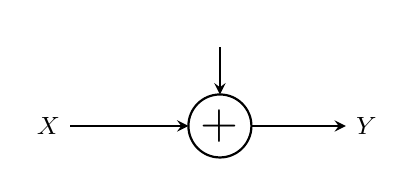
\begin{tikzpicture}
\shorthandoff{>}
%
%
% entrada
\draw[>=stealth,->,thick] (0,0) node[left]{\small $X$} --(1.5,0);
%
% adicion del ruido
\draw[thick] (1.9,0) circle (.4);
\draw[>=stealth,->,thick] (1.9,1) node[above]{\small $\Gauss$} --(1.9,.4);
\draw (1.9,0) node[align=center,scale=1.5]{\large +};
%
% salida
\draw[>=stealth,->,thick] (2.3,0)--(3.5,0) node[right]{\small $Y$};
\end{tikzpicture}
\end{center}
\leyenda{Canal gaussiano. La entrada $X$,  modelisada por un vector aleatorio es
  corrupto aditivamente por un ruido gaussiano $\Gauss$ independiente de $X$. La
  salida es entonces $Y  = X + \Gauss$ y el canal  es completamente descrito por
  $p_{Y|X}(x,y)   =    p_{\Gauss}(y-x)$   (obviamente   independiente    de   la
  distribuci\'on de la entrada).}
\label{fig:SZ:CanalGaussiano}
\end{figure}


Por  definici\'on, la informaci\'on  mutua $I(X;Y)$  entrada-salida es  dada por
$I(X;Y) = H(Y) - H(Y|X) = H(Y) - H(\Gauss)$. Maximizar $I(X;Y)$ es equivalente a
maximizar  $H(Y) =  H(X  + \Gauss)$  sujeto  a $\Tr\left(  \Sigma_X \right)  \le
P$. Fijando un  $\Sigma_X$, la propiedad~\ref{prop:SZ:cotamaximagaussiana} de le
entropia diferencial  implica que $H(Y)$  sea maximal si  y solamente si  $Y$ es
gaussiana, es decir si y solamente si $X$ est gaussiana, dando $I(X;Y) = \frac12
\log \left| \Sigma_X + \Sigma_\Gauss \right| - \frac12 \log \left| \Sigma_\Gauss
\right|$.  En conclusi\'on,  tomando  en cuenta  el  limite de  potencia, $$C  =
\max_{\frac1d \Tr   \Sigma_X  \le  P} \:  \frac12   \log\left(  \frac{\left|   \Sigma_X  +
      \Sigma_\Gauss \right|}{\left| \Sigma_X \right|} \right)$$

{\color{red} Reste a resoudre matriciel~\cite[Sec.~9.4]{CovTho06} p. 277}

En   el   caso   escalar,   se   obtiene   $$C  =   \frac12   \log\left(   1   +
  \frac{P}{\sigma_\Gauss^2}   \right)$$  donde   $\frac{P}{\sigma_\Gauss^2}$  es
conocido como relaci\'on se\~nale-ruido~\footnote{Esta formula es muy parecida a
  la   de   Shannon,    Laplume,   Clavier~\cite{Sha48,   Lap48,   Cla48}   (ver
  tambi\'en~\cite[Sec.~9.3]{CovTho06} o~\cite[Sec.~11.2]{Rio07}).   De hecho, si
  se considera simbolos mandandos durante $T$ secundos (simbolos puesto en forma
  para dar una se\~nal analogica) usando  una banda de transmisi\'on $B$, por el
  teorema de Nyquist $B = \frac{1}{2 T}$ (caso limite). Si el ruido es blanco en
  la banda $B$, de densidad espectral de potencia por unidad de frecuencia igual
  a $N_0$, para un simbolo  la relaci\'on se\~nal-ruido se escribe $\frac{P}{N_0
    B}$. Ademas,  se calcula  en general  la capacidad por  unidad de  tiempo es
  decir la  capacidad por  simbolo divido  por $T$, \ie  $C =  B \log\left(  1 +
    \frac{\sigma_X^2}{N_0 B}  \right)$ por secundos,  lo que es  precisamente la
  capacidad  calculdada por Shannon.  Esa es  a veces  conocida como  formula de
  Shannon-Hartley.}

En~\cite{CovTho06,  Rio07}  por ejemplo,  se  dan  otros  ejemplos de  canal  de
comunicaci\'on en el contexto continuo.

% ================================= codificacion

\subseccion{Codificaci\'on entropica}
\label{ss:SZ:Codificacion}


% ================================= Gaz perfecto

\subseccion{Gas perfecto}
\label{ss:SZ:Gaz perfecto}

{\color{red} Va donne lien avec Boltzmann}


% ============================== Generalizadas================================ %

\seccion{Entropias y divergencias generalizadas}
\label{s:SZ:Generalizadas}

% ================================= Salicru

\subseccion{Entropias y propiedades}
\label{ss:SZ:Salicru}

{\bf  Salicru, Buerbea-Rao,  poner  ac\'a la  codificaci\'on  a la  Renyi, y  la
  cuantificacion fina; EPI generalizada  por Madiman, etc. Lutwak, Bercher etc.,
  Kagan}

% ================================= Salicru

\subseccion{Divergencias y propiedades}
\label{ss:SZ:Czizar}

{\bf Czizar, Bregmann, Burbea Rao}


% =============================== Cuanticas ================================== %

\seccion{Entropias cuanticas discretas}
\label{s:SZ:Cuanticas}

{\bf Mas alla caso de informaciones a partir de medida; caso infinito, continuo queda en discusiones}


% ================================= Entropia ================================= %




 % Steeve
\capitulo{Elementos de geometr\'ia diferencial}{Pedro Walter Lamberti}

\begin{epigrafe}
  $\acute{\alpha}    \gamma\epsilon     \omega    \mu    \acute{\epsilon}    \mu
  \acute{\epsilon} \tau \rho \eta \tau o \varsigma \;\; \mu \eta \delta
  \epsilon \iota \varsigma \;\; \epsilon \iota \sigma \iota \tau \omega$  \\
  Que  no ingrese  nadie  que no  sepa geometr\'ia.   \autortituloepigrafe{Frase
    grabada en la entrada de la Academia de Plat\'on}
\end{epigrafe}


% =============================== Introduccion =============================== %

\seccion{Estructuras}
\label{s:WL:Introduccion}

Una  de  las  nociones m\'as  elementales  de  la  matem\'atica  es la  de  {\it
  conjunto}.   Un  conjunto  es   una  colecci\'on  de  elementos  perfectamente
caracterizados.   Los  elementos  pueden   ser  de  cualquier  tipo:  n\'umeros,
funciones, personas, autos, etc. El  enfoque matem\'atico moderno es ir montando
estructuras de  distinta naturaleza sobre  un dado conjunto. En  este cap\'itulo
comenzaremos con la noci\'on de espacio topol\'ogico y llegaremos al concepto de
variedad Riemanniana. Este procedimiento ha mostrado ser de utilidad en el marco
de la f\'isica, que es nuestro principal \'ambito de inter\'es.  El mapa de ruta
de las distintas estructuras que veremos en este cap\'itulo es el siguiente:
%
\begin{itemize}
\item Espacio topol\'ogico (continuidad)
\item Espacio m\'etrico (distancia)
\item Variedad topol\'ogica (coordenadas)
\item Variedad diferenciable (diferenciabilidad)
\item Estructura afin (paralelismo)
\item Estructura m\'etrica (Finsler y Riemann)
\end{itemize}

Si  bien   existe  una  estructura   intermedia  entre  la  topol\'ogica   y  la
diferenciable,  que se  conoce como  {\it  estructura lineal  a trozos},  aqu\'i
prescindiremos de su estudio. A  su vez, hay otras estructuras matem\'aticas que
son usadas en el marco de  las teor\'ias f\'isicas. Se destacan la estructura de
producto  interno sobre  un espacio  vectorial complejo,  la cual  conduce  a la
noci\'on  de  espacio  de  Hilbert,  de fundamental  importancia  en  mec\'anica
cu\'antica;  la estructura simpl\'ectica,  \'util en  mec\'anica cl\'asica  y la
estructura de K\"ahler, de relevancia en teor\'ia de cuerdas.

% ============================ Espacio Topologico ============================ %

%Comenzaremos con la noci\'on de espacio topol\'ogico.
%\sub
\seccion{Espacio Topol\'ogico}
\label{s:WL:EspacioTopologico}

Un conjunto  arbitrario $X$  est\'a desprovisto de  toda estructura  que permita
definir nociones tales como la {\it convergencia} de una sucesi\'on de elementos
de  $X$, la  {\it proximidad}  de dos  elementos de  $X$, etc.  En  principio se
dispone s\'olo de las operaciones  elementales de {\it uni\'on} $\bigcup$ e {\it
  intersecci\'on} $\bigcap$ de  subconjuntos. Estas operaciones tambi\'en pueden
realizarse entre  distintos conjuntos.  Denotaremos con $\emptyset$  al conjunto
vac\'io. Surge entonces el desaf\'io de construir alguna estructura matem\'atica
definida  sobre $X$  que  permita definir,  de  manera precisa  las nociones  de
proximidad, continuidad, convergencia, etc. Esto  se logra a trav\'es de la idea
de una {\bf topolog\'ia} sobre $X$.

\begin{definicion}[Topolog\'ia]
  Una  {\it topolog\'ia}  $\Upsilon$ sobre  el conjunto  $X$ es  una  familia de
  subconjuntos de $X$ que cumple con las siguientes condiciones:
  %
  \begin{enumerate}
  \item $X$ y $\emptyset$ est\'an en $\Upsilon$: $X, \emptyset \in \Upsilon$
  %
  \item  La  intersecci\'on de  cualquier  colecci\'on  finita  de elementos  de
    $\Upsilon$ est\'a en $\Upsilon$:
    \[
    A_i \in  \Upsilon, \quad \forall  \: i  = 1 ,  \ldots , n  \quad \Rightarrow
    \quad \bigcap_{i=1}^n A_i \in \Upsilon
    \]
  %
  \item La uni\'on de una colecci\'on arbitraria --finita o no-- de elementos de
    $\Upsilon$, pertenece a $\Upsilon$:
    \[
    A_i \in \Upsilon \quad \Rightarrow \quad \bigcup_i A_i \in \Upsilon
    \]
  \end{enumerate}
\end{definicion}

\begin{definicion}[Espacio topol\'ogico y abiertos]
  Al par $(X,\Upsilon)$ lo  llamaremos {\it espacio topol\'ogico}. Los conjuntos
  que est\'an en $\Upsilon$ se llaman {\it abiertos}.
\end{definicion}


%{\it 
Ejemplos:
%}:
%
\begin{itemize}
\item {\it  Topolog\'ia trivial}. Es la  que consta de s\'olo  dos elementos, el
  conjunto vac\'io y el conjunto total $X: \Upsilon = \{ \emptyset , X \}$.
%
\item {\it Topolog\'ia discreta}. Es la que en todo subconjunto de $X$ est\'a en
  $\Upsilon$, es decir $\Upsilon =  \P(X)$ donde $\P(X)$ representa a las partes
  de $X$.
%
\item En  los cursos elementales  de an\'alisis matem\'atico hemos  estudiado en
  $\Rset^n$, es decir el conjunto de $n$-tuplas de n\'umeros reales, la noci\'on
  de bolas abiertas. M\'as precisamente,  una bola abierta en $\Rset^n$ centrada
  en el punto $p = (p_1,...,p_n) \in \Rset^n$ y de radio $r > 0$ es el conjunto
  \[
  \B_{r,p} = \left\{ (x_1 , \ldots , x_n) \in \Rset^n:   \: 0 \le   \sqrt{\sum_i
      (x_i-p_i)^2} < r \right\}
  % \text{tal que} \;\; 0\leq \sqrt{\sum_i (x_i-p_i)^2}<r}
  \]
  %
  La  colecci\'on de  todas  las  bolas abiertas  en  $\Rset^n$ constituyen  una
  topolog\'ia  para $\Rset^n$.   Se conoce  como la  {\it topolog\'ia  usual} de
  $\Rset^n$.\newline Obs\'ervese que un  subconjunto $A$ de $\Rset^n$ es abierto
  (en el sentido  usual), cuando para todo  $x \in A$, existe un  $\varepsilon > 0$
  tal que $\B_{\varepsilon,x} \subset A$.
\end{itemize}

\begin{definicion}[Entorno]
  Un {\it entorno} de un punto $x \in X$ es un conjunto $U$ que contiene a $x$ y
  tal que existe un  abierto $V$ contenido en $U$: $x \in  V \subseteq U$ con $V
  \in \Upsilon$.
\end{definicion}

\begin{definicion}[Funci\'on continua]
  Sea $f: X  \rightarrow Y$ una funci\'on entre  dos espacios topol\'ogicos $(X,
  \Upsilon)$ e  $(Y,\omega)$. $f$ es una  {\bf funci\'on continua} en  $x \in X$
  sii dado cualquier entorno abierto $U  \subset Y$ de $f(x)$, existe un entorno
  de $x$,  $V \subset  X$ tal  que $f(V) \subset  U$. Equivalentemente  se puede
  definir  una  funci\'on continua  de  la siguiente  manera:  $f$  es una  {\it
    funci\'on continua}  sii la  imagen inversa de  cada conjunto abierto  es un
  abierto.
\end{definicion}
%
%Equivalentemente se puede definir una funci\'on continua de la siguiente manera:
%
%\begin{definicion}[Funci\'on continua]
%  Sea $f: X \rightarrow Y$  una funci\'on entre dos espacios topol\'ogicos $(X,
%  \Upsilon)$ e $(Y,\omega)$. $f$ es  una {\bf funci\'on continua} sii la imagen
%  inversa de cada conjunto abierto es un abierto.
%\end{definicion}
Es f\'acil demostrar la equivalencia entre ambas definiciones, y hacerlo queda como ejercicio para el lector.

\begin{definicion}[Homomorfismo]
  Un {\it homomorfismo} $\Psi$ entre dos espacios topol\'ogicos $(X,\Upsilon)$ e
  $(Y,\omega)$ es una funci\'on $\Psi: X \rightarrow V \subseteq Y$
  %
  % \[
  % \Psi: X \rightarrow V \subseteq Y
  % \]
  biyectiva, continua y con inversa continua.
\end{definicion}

\begin{definicion}[Sucesi\'on]
  Una  {\it  sucesi\'on}  en un  conjunto  $X$  es  una aplicaci\'on  $s:  \Nset
  \rightarrow   X$   donde   $\Nset$   es   el   conjunto   de   los   n\'umeros
  naturales. Denotaremos a la sucesi\'on por $\{ x_n \}_{n \in \Nset}$.
  % \text{donde } n \in \Nset$
\end{definicion}

En un espacio topol\'ogico podemos introducir la noci\'on de convergencia de una
sucesi\'on. Obs\'ervese  que \'esto  es posible gracias  a que disponemos  de la
noci\'on de conjunto abierto.

\begin{definicion}[L\'imite]
  Sea $(X,  \Upsilon)$ un espacio topol\'ogico  y $\{ x_n \}_{n  \in \Nset}$ una
  sucesi\'on en $X$. Diremos que $x$ es  el {\it l\'imite} de $x_n$ si para todo
  entorno $V$ de $x$,  existe un $n_0 \in \Nset$ tal que  $\forall n \ge n_0$ se
  tiene que $x_n \in V$.
\end{definicion}

Los l\'imites de  las sucesiones no tienen porque  ser \'unicos. Una condici\'on
que debe cumplir el espacio  topol\'ogico $(X,\Upsilon)$ para que las sucesiones
tengan un \'unico l\'imite es que  dados dos puntos distintos $x \ne y$,con $x,y
\in X$ existen entornos disjuntos de $x$ e $y$. A los espacios topol\'ogicos que
cumplen  con esta  condici\'on se  los llama  espacios de  Hausdorff  o espacios
$T_2$.


% ============================== Espacio Metrico ============================= %

%\sub
\seccion{Espacios m\'etricos}
\label{s:WL:Metrico}

En el  tercer ejemplo de espacio  topol\'ogico, usamos la  noci\'on de m\'etrica
eucl\'idea  para definir las  bolas abiertas  en $\Rset^n$.  El disponer  de una
m\'etrica  no es  algo que  ocurre  en todo  conjunto. Eso  motiva la  siguiente
definici\'on:
%
\begin{definicion}[Espacio m\'etrico]
  Un {\it  espacio m\'etrico} en un conjunto  $X$ munido de una  funci\'on $d: X
  \times X \rightarrow \Rset_+$ tal que se cumplen las condiciones:
%
\begin{enumerate}
\item $d(x,y) \ge 0 \quad \forall \: x , y \in X$ y la igualdad se cumple sii $x
  = y$,
%
\item\label{Metrica:simetria} $d(x,y) = d(y,x)$ \ simetr\'ia.
%
\item\label{Metrica:triangular} $d(x,y) \le d(x,z) +  d(z,y) \quad \forall x , y
  , z \in X$.
\end{enumerate}
\end{definicion}
%
\noindent   La   \'ultima   condici\'on   se  conoce   como   {\it   desigualdad
  triangular}.  Mas adelante  en este  libro veremos  funciones $d:  X  \times X
\rightarrow \Rset_+$ que  no satisfacen ni la condici\'on~\ref{Metrica:simetria}
ni  la condici\'on~\ref{Metrica:triangular},  pero que  sin embargo  sirven para
medir cu\'an separados est\'an dos puntos de $X$. En ese caso diremos que $d$ es
una {\it distancia} definida sobre $X$.%%% ??? DIVERGENCIA?


% ============================ Variedad Topologica =========================== %

%\sub
\seccion{Variedad Topol\'ogica}
\label{s:WL:VariedadToplogica}

Nuestra experiencia cotidiana de percibir  que estamos inmersos en un espacio de
3 dimensiones, en el cual  podemos medir \'angulos y determinar distancias entre
dos puntos, ha  hecho que usemos estas caracteristicas  de nuestro habitat, como
motivaci\'on de  la defici\'on de ciertas estructuras  matem\'aticas en espacios
abstractos.

En primer lugar, con la noci\'on de una variedad topol\'ogica buscaremos simular
en  un conjunto  cualquiera, la  noci\'on  de cercan\'ia  y dimensionalidad  que
tenemos en $\Rset^n$.

\begin{definicion}[Variedad topol\'ogica $n$-dimensional]
  Una  {\it Variedad  topol\'ogica $n$-dimensional}  es un  espacio topol\'ogico
  $\M$ tal que es {\it localmente eucl\'ideo}, es decir que para cada $x \in \M$
  existe  un  entorno  abierto $U$  de  $x$,  homeomorfo  a  un abierto  $V$  de
  $\Rset^n$: \ $\phi: U \subseteq \M \rightarrow \Rset^n$ \
  %
  % \[
  % \phi: U \subseteq \M \rightarrow \Rset^n
  % \]
  %
  tal que \ $\phi:U \rightarrow V$ \
  % \[
  % \phi:U \rightarrow V
  % \]
  y  $\phi$ es  un homeomorfismo.  Tambi\'en  pediremos que  $\M$, como  espacio
  topol\'ogico, sea un espacio Hausdorff.
\end{definicion}
%
A los pares  $(U,\phi)$ se los denominan {\it cartas sobre  $\M$}. Se supone que
la  colecci\'on de  todas las  cartas cubren  completamente a  $\M$.  Las cartas
permiten asignar {\it coordenadas} a $\M$:
%
\[
\mbox{Si}  \quad  p \in  U  \subseteq \M  \quad  \mbox{entonces}  \quad \phi:  p
\rightarrow (p_1 , \ldots , p_n) \in \Rset^n
\]

\begin{figure}[h!]
  \centerline{\includegraphics[width=13cm]{figura1.pdf}}          \leyenda{Cartas
    coordenadas usadas en la definici\'on de una variedad topol\'ogica.}
\end{figure}

A  la colecci\'on  de n\'umeros  reales $(p_1  , \ldots  , p_n)$  se  llaman las
coordenadas  de  $p$  de  acuerdo  a  la carta  $(U,\phi)$.   La  existencia  de
coordenadas, es el aspecto fundamental por el que el concepto de variedad es tan
\'util en f\'isica.

Podr\'ia suceder que un mismo punto $p$ pertenezca a m\'as de una carta, digamos
$(U_1,\phi_1)$  y  $(U_2,\psi_2)$.  En  ese  caso  hablaremos  de un  cambio  de
coordenadas:
%
\begin{equation}\label{cc}
\psi \circ \phi^{-1}: \phi(U_1 \cap U_2) \rightarrow \psi(U_1 \cap U_2)
\end{equation}
%
Si denotamos por $(p_1 , \ldots  , p_n)$ a las coordenadas correspondientes a la
carta  $(U_1,\phi_1)$  y  por  $(\tilde{p}_1  , \ldots  ,  \tilde{p}_n)$  a  las
correspondientes a la carta  $(U_2,\psi_2)$, entonces las funciones $\tilde{p}_i
= \tilde{p}_i(p_1 ,  \ldots , p_n)$ son funciones continuas, y  dan el cambio de
coordenadas. Estas funciones son invertibles con inversa continua.

Ejemplos de variedades topol\'ogicas son:
%
\begin{itemize}
\item $\Rset^n$. En este caso hay  una carta coordenada global que cubre toda la
  variedad y donde el homeomorfismo es la identidad.
%
\item $\Sset^n$, la esfera de dimensi\'on $n$. Ella est\'a definida como el conjunto:
  \[
  \Sset^n = \left\{  (x_1 , \ldots ,  x_{n+1}), \: x_i \in \Rset:  \quad x_1^2 +
    \cdots + x_{n+1}^2 = 1 \right\}
  % \text{ tales que }
  \]
\end{itemize}
%
\noindent  Se debe observar  que al  definir $\Sset^n$  no estamos  pensando que
est\'a inmersa  en $\Rset^n$. En este  caso podemos usar  las siguientes cartas:
$(U_N,  \phi_N)$ y $(U_S,\phi_S)$,  donde $U_N  = \Sset^n-\{  (0,0,\ldots,1) \},
\quad U_S = \Sset^n -{(1,0,\ldots,0)}$ y los mapas
%
\[
\phi_N:  U_N  \rightarrow  \Rset^n  /  (\phi_N(x_1  ,  \ldots  ,  n_{n+1}))_i  =
\frac{x_i}{1-x_{n+1}}
\]
%
y
%
\[
\phi_S:  U_S  \rightarrow  \Rset^n  /  (\phi_N(x_1  ,  \ldots  ,  n_{n+1}))_i  =
\frac{x_i}{1+x_{n+1}}
\]
%
Ambos mapas son homeomorfismos.  Observemos  que $\phi_N(x_1 , \ldots , x_{n+1})
= (t x_1 , \ldots , t x_n)$ y  $\phi_S(x_1 , \ldots , x_{n+1}) = (u x_1 , \ldots
,  u  x_n)$   con  $t  =  \frac{1}{1-x_{n+1}}$  y   $u  =  \frac{1}{1+x_{n+1}}$,
respectivamente.  Es directo verificar la  inyectividad pues si $(t x_1 , \ldots
, t x_n) = (t  y_1 , \ldots , t y_n) \Rightarrow x_i =  y_i \quad \forall \: i$.
Entonces  los puntos  $x$  e $y$  son  id\'enticos.  Para  ver la  suryectividad
consideremos el punto  $y = (y_1 , \ldots  , y_n) \in \Rset^n$. Si  tomamos $x =
\left( t^{-1}  y_1 ,  \ldots , t^{-1}  y_n ,  y_{n+1} \right)$ con  $t \ne  0$ e
$y_{n+1} =  t \sqrt{1-(t^{-1}  y_1)^2 - \cdots  - \left( t^{-1}  y_n \right)^2}$
vemos que para cada $y \in \Rset^n$ existe un $x \in \Sset^n$ tal que $\phi(x) =
y$.   Usando las  expresiones  expl\'citas  de $\phi_N$  y  $\phi_S$ es  directo
verificar que se trata de funciones continuas.

{\bf Nota}:  Hay propiedades de las  variedades topol\'ogicas que  no tienen que
ver con sus  caracter\'isticas locales, las que hemos dicho  son similares a las
de  $\Rset^n$,  sino con  sus  propiedades  globales.   Por ejemplo  una  esfera
$2$-dimensional es  homeomorfa a  la superficie de  una pelota de  futbol, a\'un
cuando pensemos en una pelota de futbol verdadera, la cual es una colecci\'on de
parches hexagonales  o pentagonales,  unidos unos con  otros. Ambos  objetos, la
esfera  y la pelota  de futbol,  son objetos  compactos, cerrados  y simplemente
conexos.   Sin  embargo   un  toro  y  una  esfera   no  comparten  todas  estas
caracter\'isticas: un toro  es cerrado, compacto pero no  simplemente conexo, es
decir no  todo lazo sobre  \'el puede contraerse  continuamente a un  punto. Por
ello diremos que un toro y una esfera son localmente homeomorfos, pero no lo son
globalmente. Este tipo de situaciones  ha llevado a introducir cantidades que de
alguna  manera   caractericen  a  las  propiedades  globales   de  una  variedad
topol\'ogicas. Un ejemplo muy conocido  es la caracter\'istica de Euler. Para un
poliedro de  tres dimensiones la  caracteristica de Euler $\Xi$  est\'a definida
por
%
\[
\Xi = V - A + C
\]
%
donde  $V, A$ y  $C$ son  el n\'umero  de vertices,  de aristas  y de  caras del
poliedro, respectivamente. Para un cubo,  por ejemplo, $\Xi = 2$. Supongamos que
el cubo est\'a hecho en un  material el\'astico, apoyado sobre un armaz\'on (las
aristas) de metal. Si inflamos ese cubo, obtenemos una esfera. Matem\'aticamente
eso significa que el cubo y la efera son globalmente homeomorfos entre si, y por
lo  tanto topol\'ogicamente  equivalentes. Es  posible extender  el  concepto de
caracter\'istica  de Euler  a la  superficie  de una  esfera, a  trav\'es de  la
triangularizaci\'on de  la superficie esf\'erica,  es decir cubriendo  la esfera
por tri\'angulos.  En  ese caso la caracter\'istica de Euler  se calcula como el
n\'umero  de tri\'angulos  menos el  n\'umero de  aristas m\'as  el  n\'umero de
v\'ertices. Haci\'endo  ese c\'alculo  para la esfera  resulta el valor  $2$. Lo
mismo sucede con cualquier otro poliedro que se pueda deformarse continuamente a
una  esfera.  Hay maneras  de  definir la  caracter\'istica  de  Euler para  una
variedad topol\'ogica  arbitraria y esa cantidad es  un invariante topol\'ogico,
es decir  una cantidad que no  cambia entre variedades  homeom\'orficos. Para un
toro la caracter\'istica de Euler vale $0$.


% =========================== Variedad Diferenciable ========================= %

%\sub
\seccion{Variedad Diferenciable}
\label{s:WL:VariedadDiferenciable}

Sobre una  variedad topol\'ogica  se puede ``montar''  una nueva  estructura. Es
posible  hacer  eso imponiendo  condiciones  de  diferenciabilidad  a los  mapas
coordenados de  la definici\'on  de una variedad  topol\'ogica. Sin  embargo, no
tenemos   definida  la   noci\'on   de  diferenciablidad   sobre  una   variedad
cualquiera.  Por  ello, para  definir  una  estructura  diferenciable sobre  una
variedad  topol\'ogica  arbitraria,  recurrimos  a  $\Rset^n$  donde  si  est\'a
definida la noci\'on de diferenciabilidad. Por ello hacemos la siguiente:
%
\begin{definicion}[$C^r$-compatibilidad]
  Diremos que dos cartas coordenadas  $(U,\phi)$ y $(V,\psi)$ sobre una variedad
  $\M$ son  $C^r$-compatibles si  cuando $U \bigcap  V \ne \emptyset  $ entonces
  $\phi \circ \psi^{-1}$  y $\psi \circ \phi^{-1}$ son de  clase $C^r$ sobre los
  subconjuntos  $\phi(U  \bigcap  V)$   y  $\psi(U  \bigcap  V)$  de  $\Rset^n$,
  respectivamente.
\end{definicion}
%
Con esto podemos avanzar en la siguiente:
%
\begin{definicion}[Variedad diferenciable]
  Una {\it Variedad diferenciable} $n$-dimensional  de clase $C^r$, $\M$, es una
  variedad  topol\'ogica  y una  familia  de  cartas  coordenadas $\B  =  \left(
    U_\alpha , \phi_\alpha \right)$, tales que:
  %
  \begin{enumerate}
  \item los $U_{\alpha}$ cubren $\M$,
  %
  \item  para cualquier  par $\alpha,  \beta$, los  entornos $\left(  U_\alpha ,
      \phi_\alpha \right)$  y $\left( U_\beta  , \phi_\beta \right)$  son $C^r$-
    compatibles,
  %
  \item  Cualquier   entorno  coordenado  $(V,\psi)   \:\:  C^r$-compatible  con
    cualquiera de los  $\left( U_\alpha , \phi_\alpha \right)  \in \B$ est\'a en
    $\B$.
  \end{enumerate}
\end{definicion}

\begin{figure}
 \centerline{\includegraphics[width=13cm]{figura2.pdf}}
%
 \leyenda{Cartas  coordenadas  usadas  en   la  definici\'on  de  una  funci\'on
   diferenciable.}
\end{figure}

Cualquier  superficie ``suave''  en $\Rset^3$  es un  ejemplo de  (sub) variedad
diferenciable. Este ejemplo no debe conducir  a la confusi\'on de pensar que una
variedad debe estar inmersa en $\Rset^n$. Otro ejemplo de variedad diferenciable
de dimensi\'on $n$ es la esfera $\Sset^n$, definida previamente.

\begin{definicion}[Diferenciabilidad de clase $C^k$]
  Dadas  dos variedades  $\M$ y  $\M'$ de  clase $C^r$,  una  aplicaci\'on $f:\M
  \rightarrow \M' $,  se dice {\it diferenciable} de clase $C^k,  \quad k \le r$
  si para  toda carta  $\left( U_\alpha  , \phi_\alpha \right)$  de $\M$  y toda
  carta  de $\left(  V_\beta ,  \psi_\beta \right)$  de $\M'$  tal  que $f\left(
    U_\alpha \right) \subset V_\beta$, la aplicaci\'on $\psi_\beta \circ f \circ
  \phi_\alpha^{-1}$ de $\phi_\alpha\left( U_\alpha \right)$ en $\psi_\beta\left(
    V_\beta \right)$, es diferenciable de clase $C^k$.
\end{definicion}

El disponer  de la noci\'on de  funci\'on diferenciable, permite  asignar a cada
punto de una variedad diferenciable,  un espacio vectorial. \'Este estar\'a dado
por operadores  lineales que act\'uan  sobre funciones diferenciables y  dan por
resultado un n\'umero.  Antes de ir a la definici\'on  de ese espacio vectorial,
introducimos el concepto de curva suave sobre una variedad.
%
\begin{definicion}[Curva de clase $C^k$ sobre una variedad]
  Sea $\M$  una variedad de  clase $C^r$. Una  curva $\lambda$ en $\M$  de clase
  $C^k, \quad k  \le r$ es una funci\'on  del intervalo real $[a \, ,  \, b]$ en
  $\M$ tal que  para toda carta $\left( U_\alpha ,  \phi_\alpha \right)$ en $\M$
  la composici\'on
  %
  \[
  \phi_\alpha \circ \gamma: [a \, , \, b] \rightarrow \phi_\alpha\left( U_\alpha
  \right)
  \]
  %
  es de clase $C^k$. En coordenadas
  %
  \[
  \phi_\alpha \circ \gamma (t) = \{ x^1(t) , \ldots , x^n(t) \}
  \]
\end{definicion}
%
Con esto podemos ahora dar la noci\'on de vector tangente a una variedad:
%
\begin{definicion}[Tangente a una variedad]
  Sea $\F(p)$ el  conjunto de funciones diferenciables de  clase $C^1$ definidas
  en un entorno del punto $p$.  Sea $\gamma(t)$ una curva de clase $C^1$, $a \le
  t  \le b$  tal que  $\gamma(t_0) =  p$. El  vector {\it  tangente} a  la curva
  $\gamma(t)$ en el punto $p$ es una aplicaci\'on $\mathbb{X}_p : \F(p) \rightarrow \Rset$
  % \[
  % \mathbb{X}_p : \F(p) \rightarrow \Rset
  % \]
  cuyo efecto es
  %
  \[
  \mathbb{X}_p f = \frac{df(\gamma (t))}{dt} |_{t_0}
  \]
\end{definicion}
%
El vector $\mathbb{X}_p$ satisface las siguientes propiedades
%
\begin{itemize}
 \item $\mathbb{X}_p$ es una aplicaci\'on lineal de $\F(p)$ en $\Rset$,
  %
 \item  $\mathbb{X}_p(fg) =  \left( \mathbb{X}_p  f \right)  g(p) +  f(p) \left(
     \mathbb{X}_p g \right)$ para $f , g \in \F(p)$.
\end{itemize}
%
Dejamos para el lector demostrar estas propiedades.

Sean $(u^1 , \ldots  , u^n)$ coordenadas locales en un entorno  $U$ de $p$. Para
cada $j$, $\left( \frac{\partial}{\partial  u^j} \right)|_p$ es una aplicaci\'on
de $\F(p)$  en $\Rset$ la cual satisface  las propiedades (i) e  (ii). Veremos a
continuaci\'on que el conjunto de todas las aplicaciones $\mathbb{X}$ de $\F(p)$
en $\Rset$ es un espacio vectorial $n$-dimensional, siendo $n$ la dimensi\'on de
la variedad diferenciable $\M$.

Dada una  curva $\gamma(t)$ con $\gamma(t_0)  = p$, sean  $u^j(t) = \gamma^j(t),
\quad  j =  1 ,  \ldots ,  n$  las coordenadas  locales de  esa curva.  Entonces
$\frac{df(\gamma(t))}{dt}|_{t_0}  =  \sum_j  \left(  \frac{\partial  f}{\partial
    u^j}|_p  \right)  \left( \frac{d  \gamma^j  (t)}{dt} \right)|_{t_0}$.  Extra %% ESTA???
expresi\'on indica  que todo vector  en $p$ es  una combinaci\'on lineal  de los
vectores (operadores).

\begin{equation}
\left(\frac{\partial}{\partial u^1}|_p \right),\ldots,\left(\frac{\partial}{\partial u^n}|_p \right) \label{set}
\end{equation}

Sea la  combinaci\'on lineal  $\sum_j \xi^j \frac{\partial}{\partial  u^j}|_p$ y
sea la curva definida por
%
\[
u^j(t) = u^j(p) + \xi^j t \quad j = 1 , \ldots , n
\]
%
El   vector   tangente   a   esta   curva   en  $t   =   0$   es   $\sum   \xi^j
\frac{\partial}{\partial u^j}|_p$.  Adem\'as si
%
\[
\sum \xi^j \frac{\partial}{\partial u^j}|_p =0,
\]
%
entonces
%
\[
0 = \sum \xi^j \left( \frac{\partial u^k}{\partial u^j} \right)|_p = \xi^k \quad
k = 1 , \ldots , n
\]
%
Esto demuestra la independencia lineal de los vectores~\eqref{set}.
%
\begin{definicion}[Espacio tangente]
  El conjunto  de vectores tangentes en $p  \in \M$, es llamado  el {\it espacio
    tangente de $\M$ en $p$}, y lo denotaremos por $T_p(\M)$.
\end{definicion}

La colecci\'on de todos los  espacios tangentes, $\bigcup_{p \in \M} T_p(\M)$ se
llama {\it fibrado tangente}.

Al fibrado tangente se le puede  dar la estructura de un \'algebra (\'algebra de
Lie). Esta surge de calcular  el conmutador $[\mathbb{X}, \mathbb{Y}]$ entre dos
campos vectoriales $\mathbb{X}$ e $\mathbb{Y}$:
%
\[
[\mathbb{X},  \mathbb{Y}] f  \equiv  \left( \mathbb{X}  \mathbb{Y} -  \mathbb{Y}
  \mathbb{X} \right) f
\]
%
Si los vectores  se escriben en t\'ermino de los vectores  de la base coordenada
$\left(  \frac{\partial}{\partial  x^a}  \right)$,  el  conmutador  entre  ellos
resulta ser el vector:
%
\[
\sum_{ab} X^a \frac{\partial  Y^b}{\partial x^a} \frac{\partial}{\partial x^b} -
\sum_{ab} Y^a \frac{\partial X^b}{\partial x^a} \frac{\partial}{\partial x^b}
\]

A cada espacio tangente $T_p(\M)$ podemos asignar su dual, $T_p^*(\M)$, es decir
el conjunto de  todos los operadores lineales y  homog\'eneos que act\'uan sobre
$T_p(\M)$.   A    un   elemento   del   espacio   dual    lo   llamaremos   {\it
  $1$-forma}. Denotaremos a  la acci\'on de un elemento  de $T_p^*(\M)$, digamos
$\omega_p$, por:
%
\[
\omega_p(\mathbb{X}_p) = \left\langle \omega_p , \mathbb{X}_p \right\rangle.
\]
%
Para cada  funci\'on $f \in  \F(p)$, el {\it  diferencial de $f$},  denotado por
$(df)_p$, es el elemento de $T_p^*(\M)$ que tiene por acci\'on:
%
\[
\left\langle (df)_p ,  \mathbb{X}_p \right\rangle = \mathbb{X}_p f,  \quad \mathbb{X}_p \in
T_p(\M)
\]

Cada funci\'on coordenada $u^j$ es una funci\'on de $\M$ sobre $\Rset$. Entonces
podemos  calcular  el  diferencial  de  $u^j$, cuya  acci\'on  sobre  un  vector
$\mathbb{X}_p \in T_p(\M)$ est\'a dada por
%
\[
 \left\langle (du^j)_p , \mathbb{X}_p \right\rangle = \mathbb{X}_p^j
\]
%
En particular,  si $\mathbb{X}_p =  \left(\frac{\partial}{\partial u^k} \right)$
resulta
%
\[
\left\langle   (du^j)_p   ,   \left(   \frac{\partial}{\partial   u^k}   \right)
\right\rangle = \delta_k^j;
 \]
%
 es decir $\left\{ (du^j)_p \right\}_{j=1}^n$ es la base dual de $\left\{ \left(
     \frac{\partial}{\partial  u^j} \right)_p \right\}_{j=1}^n$.  Toda $1$-forma
 $\omega$ se puede escribir en t\'ermino de esta base:
%
\[
\omega = \sum_a \omega_a dx^a
\]

Con los espacios  $T_p(\M)$ y $T_p^*(\M)$ podemos construir  el espacio producto
cartesiano
%
\[
\left(  T_p(\M)  \right)_s^r =  T_p(\M)  \times  T_p(\M)  \ldots T_p(\M)  \times
T_p^*(\M) \times T_p^*(\M) \ldots \times T_p^*(\M)
\]
%
con $r$ factores de $T_p(\M)$ y $s$ factores de $T_p^*(\M)$.

\begin{definicion}[Tensor de tipo $(r,s)$]
  Un {\it tensor de tipo $(r,s)$} es un operador $S$,
  %
  \[
  S: \left( T_p(\M) \right)_s^r \rightarrow \Rset
  \]
  %
  que es lineal y homog\'eneo en cada uno de sus argumentos.
\end{definicion}

\begin{definicion}[Campo tensorial]
  Un {\it campo tensorial $S$ de  clase $C^k$ de tipo $(r,s)$ sobre $V \subseteq
    \M$} es un mapa  $C^k$ que asigna un tensor de tipo  $(r,s)$ a cada punto $p
  \in V$.
\end{definicion}
%
En  t\'ermino  de las  bases  $\left\{  \left( \frac{\partial}{\partial  u^j}|_p
  \right)  \right\}_{j=1}^n$  y $\left\{  (du^j)_p  \right\}_{j=1}^n$, el  campo
tensorial $S$ se puede escribir:
%
\[
S(p) = S^{a_1 \ldots  a_r}_{b_1 \ldots b_s}(p) \frac{\partial}{\partial x^{a_1}}
\bigotimes   \ldots  \bigotimes  \frac{\partial}{\partial   x^{a_r}}  \bigotimes
dx^{b_1} \bigotimes \ldots \bigotimes dx^{b_s}
\]
%
\noindent donde  las funciones $S^{a_1 \ldots a_r}_{b_1 \ldots b_s}$  son de clase
$C^k$ y $\bigotimes$ es el producto tensorial.

Entre los campos tensoriales que se  pueden definir sobre una variedad $\M$, hay
uno particularmente importante,  y es conocido como el  tensor m\'etrico. \'Este
se define por medio de un producto escalar:
%
\begin{definicion}[Producto escalar]
  Un {\bf producto escalar} sobre $T_p(\M)$ es una funci\'on
  %
  \[
  g: T_p(\M) \times T_p(\M) \rightarrow \Rset
  \]
  %
  que satisface
  %
  \begin{enumerate}
  \item $g(\mathbb{X}, \mathbb{Y}) = g(\mathbb{Y}, \mathbb{X}), \quad \text{para}
    \quad \mathbb{X}, \mathbb{Y} \in T_p(\M)$
  %
  \item  $g(\mathbb{X},   a  \mathbb{Y}  +  b  \mathbb{Z})   =  a  g(\mathbb{X},
    \mathbb{Y}) + b g(\mathbb{X}, \mathbb{Z})$
  \end{enumerate}
\end{definicion}

El producto escalar se dice  {\it no degenerado} si $g(\mathbb{X}, \mathbb{Y})=0
\quad \forall \:  \mathbb{Y} \in T_p(\M)$ implica $\mathbb{X}  = 0$.  Obviamente
el  producto  escalar  es un  tensor  de  tipo  $(0,2)$.  Como  campo  tensorial
$g(\;,\;)$   se   puede   expresar    en   t\'erminos   de   la   base   $\left(
  \frac{\partial}{\partial    u^1}|_p     \right)    ,    \ldots     ,    \left(
  \frac{\partial}{\partial u^n}|_p \right)$
%
\[
g(\mathbb{X}, \mathbb{Y})  = \sum_{ab} X^a  Y^b g\left( \frac{\partial}{\partial
    u^a}, \frac{\partial}{\partial u^b} \right)
\]
%
o, de manera equivalente
%
\[
g(\mathbb{X}, \mathbb{Y}) = \sum_{ab} g_{ab} X^a Y^b
\]
%
donde     $g_{ab}    =    g     \left(    \frac{\partial}{\partial     u^a}    ,
  \frac{\partial}{\partial  u^b}   \right)$.  Si  el  producto   escalar  es  no
degenerado, entonces  existe la  matriz inversa de  la matriz $g_{ab}$,  a cuyos
elementos los denotaremos por $g^{ab}$, de modo que
%
\[
\sum_c g_{ac} g^{cb} = \delta_a^b
\]

La  existencia de  un campo  tensorial  m\'etrico (o  producto escalar  definido
localmente),  permite introducir  la idea  de {\it  longitud de  una  curva}. En
efecto, sea  $\gamma(t), \quad t  \in [a \,  , \, b]$  una curva de  clase $C^1$
sobre $\M$,  que une los  puntos $p$  y $q$: $\gamma(a)  = p, \quad  \gamma(b) =
q$. En el punto $\gamma(t)$ tenemos  el vector tangente a la curva $\gamma$ dado
por
%
\[
\left( \frac{\partial}{\partial t} \right)_\gamma = \sum_j \frac{d \gamma^j}{dt}
\frac{\partial}{\partial x^j}
\]

\begin{definicion}[Longitud de una curva]
  La {\it longitud de la curva $\gamma$  entre los puntos $p$ y $q$} est\'a dada
  por la cantidad
  %
  \begin{equation}
    L = \int_a^b | g \left( \frac{\partial}{\partial t}, \frac{\partial}{\partial t} \right) |^{\frac{1}{2}} dt
  \label{longitud}
  \end{equation}
\end{definicion}
%
O, equivalentemente
%
\begin{equation}
L = \int_a^b \left| \sum_{ij} g_{ij}(x) \frac{d\gamma^i}{dt} \frac{d \gamma^j
}{dt} \right|^{\frac{1}{2}} dt \label{longitud}
\end{equation}

% ============================== Estructura Afin ============================= %

%\sub
\seccion{Estructura Afin}
\label{s:WL:EstructuraAfin}

En  el espacio  eucl\'ideo  $n$-dimensional (pensado  aqu\'i  como una  variedad
diferenciable),  cuando  usamos coordenadas  cartesianas,  caracterizamos a  dos
vectors paralelos como aquellos  que tienen iguales componentes. Si reemplazamos
las coordenadas cartesianas por las polares, por ejemplo, esta caracterizaci\'on
deja  de  ser  v\'alida.  Veamos   c\'omo  podemos  introducir  la  noci\'on  de
paralelismo de vectores, usando  cualquier sistema de coordenadas. Sea $\{x^a\}$
el sistema de  coordenadas cartesiano del espacio. En  este sistema, hemos dicho
que  dos vectores  paralelos,  por ejemplo  $\mathbb{V}$ y  $\tilde{\mathbb{V}}$
tienen iguales componentes:
%
\[
V^a = \tilde{V}^a
\]
%
Si el vector $\mathbb{V}$ es tangente al espacio en el punto $p$ con coordenadas
$\{ x^a \}$  y el vector paralelo $\tilde{\mathbb{V}}$ es  tangente al punto $q$
con coordenadas ${x^a+\delta x^a}$, vale
%
\[
\tilde{V}^a(q)-V^a(p) = 0
\]
%
Dado  un  vector $\mathbb{V}$  en  $p$, podemos  definir  un  campo de  vectores
paralelos  a $\mathbb{V}$  en un  entorno  de $p$.  Denotemos a  este campo  por
$\tilde{\mathbb{V}}$.  Este  campo cumple  que  en  el  punto $p$  coincide  con
$\mathbb{V}$ y con la condici\'on:
%
\[
\tilde{V}^a(x+\delta x) -  V^a(x) = \frac{\partial \tilde{V}^a}{\partial x^b}(p)
\delta x^b
\]
%
Sea ${\xi^a}$ otro sistema de  coordenadas para el espacio eucl\'ideo, vinculado
con ${x^a}$ mediante las relaciones
%
\begin{equation}
\xi^a = \xi^a(x^b), \quad x^b=x^b(\xi^a) \label{cambcoor}
\end{equation}
%
A partir de ellas, resulta
%
\begin{equation}
\delta \xi^a = \frac{\partial \xi^a}{\partial x^b} \delta x^b, \qquad \delta x^b = \frac{\partial x^b}{\partial \xi^a} \delta \xi^a
\end{equation}
%
Las componentes de $\tilde{\mathbb{V}}$ se transforman de acuerdo con
%
\[
\tilde{V}^a = \frac{\partial x^a}{\partial \xi^b} \tilde{V'}^b
\]
%
donde  $\tilde{V'}^a$  son  las   componentes  de  $\tilde{\mathbb{V}}$  en  las
coordenadas $\{\xi^a\}$. Entonces, podemos escribir
%
\begin{eqnarray}
\frac{\partial \tilde{V}^a}{\partial x^b} &=& \frac{\partial}{\partial \xi^c} \left(\frac{\partial x^a}{\partial \xi^d} \tilde{V'}^d \right) \frac{\partial \xi^c}{\partial x^b}  \nonumber \\
%
& = & \frac{\partial^2 x^a}{\partial \xi^c \partial \xi^d} \tilde{V'}^d \frac{\partial \xi^c}{\partial x^a}+ \frac{\partial x^a}{\partial \xi^d} \frac{\partial{\tilde{V'}^d}}{\partial \xi^c} \frac{\partial \xi^c}{\partial x^b}
\end{eqnarray}
%
Si    definimos   la    cantidad   $\delta    \tilde{V'}^d    =   \frac{\partial
  \tilde{V'}^d}{\partial x^e} \delta \xi^e$ y despu\'es de un poco de \'algebra,
llegamos a la relaci\'on
%
\begin{equation}
\delta \tilde{V'}^n = - \frac{\partial^2 x^a}{\partial \xi^e \partial \xi^d} \frac{\partial \xi^n}{\partial x^a} \tilde{V'}^d \delta \xi^e \label{con}
\end{equation}
%
Esta expresi\'on puede reescribirse de la siguiente forma:
%
\begin{equation}
\delta \tilde{V'}^n = - \Gamma'^n_{ed} \tilde{V'}^d \delta \xi^e
\end{equation}
%
\noindent  en   donde  los  coeficientes  $\Gamma'$  est\'an   definidos  en  la
expresi\'on~\eqref{con}. De su definici\'on resulta que las cantidades $\Gamma'$
se anulan para cambios {\it lineales} de coordenadas~\eqref{cambcoor}.

Obs\'ervese que al haber arribado a la definici\'on de los coeficientes $\Gamma$
no hemos hecho uso de ninguna  propiedad especial del espacio eucl\'ideo. Es por
ello  que  la  expresi\'on~\eqref{con}   es  v\'alida  para  cualquier  variedad
n-dimensional. Es f\'acil ver que frente a un cambio de coordenadas
%
\begin{equation}
x^a \rightarrow x'^a= x'^a\left(x^b\right) \label{camb2}
\end{equation}
%
las cantidades $\Gamma$ cambian seg\'un la expresi\'on
%
\begin{equation}
\Gamma ^f_{de} = \Gamma'^a_{mn} \frac{\partial x^f}{\partial x'^a} \frac{\partial x'^m}{\partial x^d} \frac{\partial x'^n}{\partial x^e}+\frac{\partial x^f}{\partial x'^a} \frac{\partial^2 x'^a}{\partial x^e \partial x^d} \label{camcon}
\end{equation}
%
Debemos  remarcar que  esta  ley  de transformaci\'on  es  lineal y  homog\'enea
(tensorial)   s\'olo  cuando  el   cambio  de   coordenadas~\eqref{cambcoor}  es
lineal. Esta propiedad  de los coeficientes $\Gamma$ nos  permite generalizar la
idea de paralelismo en una variedad arbitraria:
%
\begin{definicion}[Conexi\'on af\'in]
  Cuando  en una  variedad  n-dimensional arbitraria  $\M$  se introducen  $n^3$
  coeficientes $\Gamma$ que se transforman de acuerdo con la ley~\eqref{camcon},
  diremos que sobre esa variedad se ha definido una {\it conexi\'on af\'in}
\end{definicion}

A partir de los coeficientes $\Gamma$ es posible definir una nueva derivada para
un campo vectorial arbitrario, digamos $V^a(x)$:
%
\begin{definicion}[Derivada covariante de campo]
  Sea  un campo vectorial  $V$ definido  en un  entorno del  punto $x$.  La {\it
    derivada covariante  del campo  $V$} est\'a dado  por las componentes  de un
  tensor de tipo $(1,1)$
  %
  \[
  V^a_{;c} = V^a_{,c} + \Gamma^a_{bc} V^b
  \]
\end{definicion}

\begin{definicion}[Derivada covariante en una direcci\'on]
  Dados dos campos  vectoriales $U(x)$ y $V(x)$, la  {\it derivada covariante de
    $V$ en la direcci\'on de $U$} es el campo vectorial definido por
  %
  \[
  U(x) \cdot \nabla V(x) \equiv \sum_{ab} V^a_{;b}(x) U^b(x) \mathbb{E}_a \equiv
  \nabla_U V
  \]
% hdot => cdot?
\end{definicion}
%
donde  $\mathbb{E}^a$ es  el campo  de  vectores coordenados  asociados con  las
coordenadas $x^a$. Esta \'ultima  definici\'on permite trasladar paralelamente a
un vector a  lo largo de una  curva. Basta con tomar como  $\mathbb{U}$ al campo
tangente a la curva.


% ============================== Variedad Riemanniana ============================= %

%\sub
\seccion{Variedad Riemmanniana}
\label{s:WL:VariedadRiemmanniana}

Sea $\M$ una variedad diferenciable  $n$-dimensional. Si $\M$ tiene definida una
m\'etrica  no   singular  sobre  ella,   recibe  el  nombre  de   {\it  variedad
  Riemanniana}. La existencia de una m\'etrica sobre $\M$ permite introducir una
conexi\'on af\'in  particular, conocida como la conexi\'on  de Levi-Civita. Sean
$g_{ab}$ y  $g^{ab}$ los coeficientes de la  m\'etrica $g$ y su  inversa, en las
coordenadas $\{x^a\}$, respectivamente.

Para  dos puntos  pr\'oximos,  la separaci\'on  entre  ellos viene  dada por  la
expresi\'on:
%
\begin{equation}
ds^2 = \sum_{ab} g_{ab} dx^a dx^b \label{quad}
\end{equation}

Adem\'as de definir una distancia  entre puntos pr\'oximos, la existencia de una
m\'etrica  permite   definir  una  conexi\'on  particular   sobre  una  variedad
riemanniana:
%
\begin{definicion}[Conexi\'on de Levi-Civita]
  La conexi\'on de Levi-Civita en las coordenadas $x^a$ est\'a dada por:
  %
  \begin{equation}
  \Gamma^a_{bc} = \frac{1}{2} \sum_d g^{ad} \left(g_{bd,c} + g_{cd.b} - g_{bc.d} \right) \label{levi}
  \end{equation}
\end{definicion}

La existencia  de esta  particular conexi\'on no  imposibilita la  existencia de
otras conexiones definidas sobre $\M$.

Como hemos visto  m\'as arriba, el tener definida  una m\'etrica permite definir
la  longitud de  una curva.  Bajo ciertas  condiciones, que  supondremos  que se
satisfacen, podemos plantearnos el problema  de determinar la curva que minimiza
(en  realidad  extremiza)  su  longitud  al  unir  dos  puntos  fijos  sobre  la
variedad. Esto se puede tratar  resolviendo el problema variacional asociado con
el funcional~\eqref{longitud}. La ecuaci\'on de Euler-Lagrange  conduce en este
caso a:
%
\begin{equation}
\frac{d^2 x^d}{dt^2} + \Gamma^d_{ca} \frac{dx^c}{dt} \frac{dx^a}{dt} = 0 \label{geode}
\end{equation}
%
\noindent donde $x^a(t)$ son las coordenadas de la curva y $t$ es un par\'ametro
adecuadamente elegido. Una curva  que satisface~\eqref{geode}, se llama una {\it
  curva geod\'esica}.  Es posible caracterizar  a una curva geod\'esica  de otro
modo. Sea  $\mathbb{U}(t)$ el vector  tangente a una curva  $\gamma(t)$ definida
sobre $\M$.  La curva $\gamma$ se  dice una geod\'esica si su vector tangente es
trasladado paralelamente a lo largo de ella:
%
\[
\mathbb{U} \cdot \nabla \mathbb{U} = f(t) \mathbb{U}
\]
% 
% hdot => cdot?
Siempre es posible  elegir al par\'ametro $t$ de forma tal  que $f(t)=0$, con lo
cual reobtenemos la ecuaci\'on~\eqref{geode}.

El disponer de geod\'esicas, permite dar a una variedad riemanniana el car\'cter
de espacio m\'etrico.  En efecto, podemos definir la  distancia entre dos puntos
$p$ y $q$ de la variedad $\M$ a trav\'es de la expresi\'on:
%
\begin{equation}
d(p,q) = \min_{\gamma} L(\gamma) \label{distt}
\end{equation}
%
\noindent donde  el m\'inimo  se eval\'ua  entre todas las  curvas que  unen los
puntos $p$ y $q$, y $L$ es la longitud~\eqref{longitud}. Como siempre, todo esto
es  posible ser  realizado  localmente.   Las geod\'esicas  son  las curvas  que
localmente  minimizan  la distancia  entre  dos  puntos.  La distancia  definida
por~\eqref{distt}  verifica  la  desigualdad   triangular,  y  por  eso  es  una
m\'etrica.

Dada una conexi\'on  $\nabla$ se define un tensor de  tipo $(1,3)$, llamado {\it
  tensor de curvatura} asociado a la conexi\'on $\nabla$, cuya espresi\'on es:
%
\[
\R\left( \mathbb{X} , \mathbb{Y} \right) \mathbb{Z} = \nabla_{\mathbb{X}} \left(
  \nabla_{\mathbb{Y}}   \mathbb{Z}    \right)   -   \nabla_{\mathbb{Y}}   \left(
  \nabla_{\mathbb{X}}  \mathbb{Z}   \right)  -  \nabla_{[\mathbb{X},\mathbb{Y}]}
\mathbb{Z}
\]
%
Si los  vectores $\mathbb{X}$, $\mathbb{Y}$ y $\mathbb{Z}$  son reemplazados por
los       vectors       coordenados       $\frac{\partial}{\partial       x^a}$,
$\frac{\partial}{\partial     x^b}$    y     $\frac{\partial}{\partial    x^c}$,
respectivamente, resulta
%
\[
\R\left( \frac{\partial}{\partial  x^a} , \frac{\partial}{\partial  x^b} \right)
\frac{\partial}{\partial x^c} = R^d_{cab} \frac{\partial}{\partial x^d}
\]
%
con
%
\[
R^d_{cba}   \equiv  \left(  \frac{   \partial  \Gamma^d_{cb}}{\partial   x^a}  +
  \Gamma^d_{ra} \Gamma^r_{cb}  - \frac{ \partial  \Gamma^d_{ca}}{\partial x^b} -
  \Gamma^d_{rb} \Gamma^r_{ca}\right) \frac{\partial}{\partial x^d}
\]

{\bf  Nota:} Si  bien existe  una motivaci\'on  geom\'etrica para  introducir el
tensor de curvatura, aqu\'i no la hemos  dado. Ella tiene que ver con la idea de
cu\'anto cambia un  vector al desplazarlo paralelamente a lo  largo de una curva
cerrada. En general diremos que una  variedad es plana, si todas las componentes
de su tensor de curvatura, se anulan.

Concluimos  este cap\'itulo  con una  breve  nota hist\'orica.  En sus  trabajos
originales sobre geometr\'ia, B. Riemann  introdujo el elemento de l\'inea entre
dos puntos vecinos $p$ y $q$ por medio de la expresi\'on
\begin{equation}
ds = F(p, \mathbb{X})dt \label{linea}
\end{equation}
%
con $F(  p , \mathbb{X} )$  una funci\'on homog\'enea  de grado 2 en  la segunda
variable. Aqu\'i estamos suponiendo que  los puntos $p$ y $q$ tienen coordenadas
${x^a}$  y ${x^a +  X^a dt}$,  respectivamente. La  geometr\'ia basada  sobre el
elemento de l\'inea  se conoce como geometr\'ia de  Finsler.  Obs\'ervese que el
elemento~\eqref{quad} (de  Riemann) es un  caso particular de la  geometr\'ia de
Finsler.

 % Walter
\capitulo{Geometr\'ia de la informaci\'on}{}


% Epigrafe de capitulo
\begin{epigrafe}
  \textcolor{red}{Esto es  un ep\'igrafe con  texto simulado.\\ Esto es  un ep\'grafe
    con  texto simulado.
\autortituloepigrafe{Autor del ep\'igrafe, T\'itulo de la obra}
}
\end{epigrafe}


\seccion{La Secci\'on 4.1}
\label{s:4.1}

Este es un  p\'arrafo Normal con texto simulado, (Arial  10, interlineado de 1,5
l\'ineas, sangr\'ia en primera l\'inea de 0,5cm. Este es un p\'arrafo Normal con
texto simulado,  (Arial 10, interlineado  de 1,5 l\'ineas, sangr\'ia  en primera
l\'inea de 0,5cm). Este es un  p\'arrafo Normal con texto simula- do, (Arial 10,
interlineado de 1,5 l\'ineas, sangr\'ia en primera l\'inea de 0,5cm). Este es un
p\'arrafo Normal  con texto simulado,  (Arial 10, interlineado de  1,5 l\'ineas,
sangr\'ia en primera  l\'inea de 0,5cm).  Este es un  p\'arrafo Normal con texto
simulado, (Arial 10, interlineado de  1,5 l\'ineas, sangr\'ia en primera l\'inea
de 0,5cm)\notaalpie{Eso es una footnote sobre varias lineas. Eso es una footnote
  sobre varias  lineas.  Eso  es una  footnote sobre varias  lineas. Eso  es una
  footnote sobre varias lineas. Eso es  una footnote sobre varias lineas. Eso es
  una footnote sobre varias lineas. Eso es una footnote sobre varias lineas. Eso
  es  una  footnote  sobre varias  lineas.  Eso  es  una footnote  sobre  varias
  lineas. Eso es una footnote sobre varias lineas.}.

% citas (de mas de 40 palabras)) ==============================================
\begin{citas}
  {\color{red} Esto  es un ejemplo  de cita  de mas de  40 palabras. Esto  es un
    ejemplo de cita de mas de 40 palabras.  Esto es un ejemplo de cita de mas de
    40 palabras. Esto  es un ejemplo de cita  de mas de 40 palabras.  Esto es un
    ejemplo de cita de mas de 40 palabras.}
\end{citas}

Este es un  p\'arrafo Normal con texto simulado, (Arial  10, interlineado de 1,5
l\'ineas, sangr\'ia en primera l\'inea de 0,5cm. Este es un p\'arrafo Normal con
texto simulado,  (Arial 10, interlineado  de 1,5 l\'ineas, sangr\'ia  en primera
l\'inea de 0,5cm). Este es un  p\'arrafo Normal con texto simula- do, (Arial 10,
interlineado de 1,5 l\'ineas, sangr\'ia en primera l\'inea de 0,5cm). Este es un
p\'arrafo Normal  con texto simulado,  (Arial 10, interlineado de  1,5 l\'ineas,
sangr\'ia en  primera l\'inea de 0,5cm).  Este es un p\'arrafo  Normal con texto
simulado, (Arial 10, interlineado de  1,5 l\'ineas, sangr\'ia en primera l\'inea
de 0,5cm).

\begin{figure}[h!]
\centerline{\includegraphics[width=2cm]{logo_large}}
%
\leyenda{Eso es  una figura, con  su leyenda sobre  varias lineas para  ver como
  queda en el texto. Eso es una  figura, con su leyenda sobre varias lineas para
  ver como queda en el texto.}
\end{figure}

Este es un  p\'arrafo Normal con texto simulado, (Arial  10, interlineado de 1,5
l\'ineas, sangr\'ia en primera l\'inea de 0,5cm. Este es un p\'arrafo Normal con
texto simulado,  (Arial 10, interlineado  de 1,5 l\'ineas, sangr\'ia  en primera
l\'inea de 0,5cm). Este es un  p\'arrafo Normal con texto simula- do, (Arial 10,
interlineado de 1,5 l\'ineas, sangr\'ia en primera l\'inea de 0,5cm). Este es un
p\'arrafo Normal  con texto simulado,  (Arial 10, interlineado de  1,5 l\'ineas,
sangr\'ia en  primera l\'inea de 0,5cm).  Este es un p\'arrafo  Normal con texto
simulado, (Arial 10, interlineado de  1,5 l\'ineas, sangr\'ia en primera l\'inea
de 0,5cm).

\begin{table}
\leyenda{Eso es un ejemplo de tabla}
\begin{center}
\begin{tabular}{|c|c|c|}
\hline
{\bf T\'itulo (negrita)} & {\bf T\'itulo (negrita)} & {\bf T\'itulo (negrita)}\\
\hline
A & Texto simulado (normal) & Texto simulado (normal)\\
\hline
B & Texto simulado (normal) & Texto simulado (normal)\\
\hline
\end{tabular}
\fuente{Eso ser\'ia el fuente de la tabla}
\end{center}\end{table}

\

Ejemplo con respecto al capitulo~\ref{cap:teoriaprobabilidades}

Para ver que las referencias de capitulos andan:~\ref{cap:teoriaprobabilidades};
que      las       de      secciones      tambi\'en~\ref{sec:var_aleat},      de
subsecciones~\ref{subsec:var_aleat_sub},                                       de
subsubsecciones~\ref{subsubsec:var_aleat_subsub}, de figuras~\ref{fig:figura}, y
de tablas~\ref{tab:tabla}.

Eso es una cita, para ver como queda~\cite{CovTho06, AmaNag00}.
 % ?
\input{Aplicaciones} % ?


% Conclusi�n general
\begin{preliminar}{Epil\'ologo}
\begin{itemize}
\item[] Este  libro surge  de la experiencia  de los  autores en el  dictado del
  curso semestral ''M\'etodos de geometr\'{\i}a diferencial en teor\'{\i}a de la
  informaci\'on",  que se  imparte  en la  Facultad  de Ciencias  Exactas de  la
  Universidad  Nacional  de   La  Plata  y  en  la   Facultad  de  Matem\'atica,
  Astronom\'{\i}a y F\'{\i}sica de la Universidad Nacional de C\'ordoba.  ...

\end{itemize}
\firma{Los autores}
\end{preliminar}

% Bibliografia - a�adir en nocite los que queremos poner y que no son citados
%\nocite{Fel71,JohKot97,JohKot95:v2,JohKot92,KotBal00}
\bibliografia{LibroIG}


% Los autores
\begin{losautores}
\elautor{Lamberti, Pedro Walter}{\input{Lamberti}}
\elautor{Portesi, Mariela}{Este es  un p�rrafo Normal  con texto simulado,  (Arial 10, interlineado  de 1,5
l�neas, sin  sangr�a en la primera l�nea).  Este es un p�rrafo  Normal con texto
simulado,  (Arial 10,  interlineado de  1,5 l�neas,  sin sangr�a  en  la primera
l�nea). Este es un p�rrafo Normal con texto simulado, (Arial 10, interlineado de
1,5 l�neas,  sin sangr�a  en la primera  l�nea). Este  es un p�rrafo  Normal con
texto simulado, (Arial 10, interlineado de 1,5 l�neas, sin sangr�a en la primera
l�nea).
}
\elautor{Zozor, Steeve}{\input{Zozor}}
\end{losautores}

\end{document}
